%********************************************%
%*       Generated from PreTeXt source      *%
%*       on 2025-01-14T16:10:29-05:00       *%
%*   A recent stable commit (2022-07-01):   *%
%* 6c761d3dba23af92cba35001c852aac04ae99a5f *%
%*                                          *%
%*         https://pretextbook.org          *%
%*                                          *%
%********************************************%
\documentclass[oneside,10pt,]{article}
%% Custom Preamble Entries, early (use latex.preamble.early)
%% Default LaTeX packages
%%   1.  always employed (or nearly so) for some purpose, or
%%   2.  a stylewriter may assume their presence
\usepackage{geometry}
%% Some aspects of the preamble are conditional,
%% the LaTeX engine is one such determinant
\usepackage{ifthen}
%% etoolbox has a variety of modern conveniences
\usepackage{etoolbox}
\usepackage{ifxetex,ifluatex}
%% Raster graphics inclusion
\usepackage{graphicx}
%% Color support, xcolor package
%% Always loaded, for: add/delete text, author tools
%% Here, since tcolorbox loads tikz, and tikz loads xcolor
\PassOptionsToPackage{dvipsnames,svgnames,table}{xcolor}
\usepackage{xcolor}
%% begin: defined colors, via xcolor package, for styling
%% end: defined colors, via xcolor package, for styling
%% Colored boxes, and much more, though mostly styling
%% skins library provides "enhanced" skin, employing tikzpicture
%% boxes may be configured as "breakable" or "unbreakable"
%% "raster" controls grids of boxes, aka side-by-side
\usepackage{tcolorbox}
\tcbuselibrary{skins}
\tcbuselibrary{breakable}
\tcbuselibrary{raster}
%% We load some "stock" tcolorbox styles that we use a lot
%% Placement here is provisional, there will be some color work also
%% First, black on white, no border, transparent, but no assumption about titles
\tcbset{ bwminimalstyle/.style={size=minimal, boxrule=-0.3pt, frame empty,
colback=white, colbacktitle=white, coltitle=black, opacityfill=0.0} }
%% Second, bold title, run-in to text/paragraph/heading
%% Space afterwards will be controlled by environment,
%% independent of constructions of the tcb title
%% Places \blocktitlefont onto many block titles
\tcbset{ runintitlestyle/.style={fonttitle=\blocktitlefont\upshape\bfseries, attach title to upper} }
%% Spacing prior to each exercise, anywhere
\tcbset{ exercisespacingstyle/.style={before skip={1.5ex plus 0.5ex}} }
%% Spacing prior to each block
\tcbset{ blockspacingstyle/.style={before skip={2.0ex plus 0.5ex}} }
%% xparse allows the construction of more robust commands,
%% this is a necessity for isolating styling and behavior
%% The tcolorbox library of the same name loads the base library
\tcbuselibrary{xparse}
%% The tcolorbox library loads TikZ, its calc package is generally useful,
%% and is necessary for some smaller documents that use partial tcolor boxes
%% See:  https://github.com/PreTeXtBook/pretext/issues/1624
\usetikzlibrary{calc}
%% We use some more exotic tcolorbox keys to restore indentation to parboxes
\tcbuselibrary{hooks}
%% Save default paragraph indentation and parskip for use later, when adjusting parboxes
\newlength{\normalparindent}
\newlength{\normalparskip}
\AtBeginDocument{\setlength{\normalparindent}{\parindent}}
\AtBeginDocument{\setlength{\normalparskip}{\parskip}}
\newcommand{\setparstyle}{\setlength{\parindent}{\normalparindent}\setlength{\parskip}{\normalparskip}}%% Hyperref should be here, but likes to be loaded late
%%
%% Inline math delimiters, \(, \), need to be robust
%% 2016-01-31:  latexrelease.sty  supersedes  fixltx2e.sty
%% If  latexrelease.sty  exists, bugfix is in kernel
%% If not, bugfix is in  fixltx2e.sty
%% See:  https://tug.org/TUGboat/tb36-3/tb114ltnews22.pdf
%% and read "Fewer fragile commands" in distribution's  latexchanges.pdf
\IfFileExists{latexrelease.sty}{}{\usepackage{fixltx2e}}
%% shorter subnumbers in some side-by-side require manipulations
\usepackage{xstring}
%% Footnote counters and part/chapter counters are manipulated
%% April 2018:  chngcntr  commands now integrated into the kernel,
%% but circa 2018/2019 the package would still try to redefine them,
%% so we need to do the work of loading conditionally for old kernels.
%% From version 1.1a,  chngcntr  should detect defintions made by LaTeX kernel.
\ifdefined\counterwithin
\else
    \usepackage{chngcntr}
\fi
%% Text height identically 9 inches, text width varies on point size
%% See Bringhurst 2.1.1 on measure for recommendations
%% 75 characters per line (count spaces, punctuation) is target
%% which is the upper limit of Bringhurst's recommendations
\geometry{letterpaper,total={340pt,9.0in}}
%% Custom Page Layout Adjustments (use publisher page-geometry entry)
%% This LaTeX file may be compiled with pdflatex, xelatex, or lualatex executables
%% LuaTeX is not explicitly supported, but we do accept additions from knowledgeable users
%% The conditional below provides  pdflatex  specific configuration last
%% begin: engine-specific capabilities
\ifthenelse{\boolean{xetex} \or \boolean{luatex}}{%
%% begin: xelatex and lualatex-specific default configuration
\ifxetex\usepackage{xltxtra}\fi
%% realscripts is the only part of xltxtra relevant to lualatex 
\ifluatex\usepackage{realscripts}\fi
%% end:   xelatex and lualatex-specific default configuration
}{
%% begin: pdflatex-specific default configuration
%% We assume a PreTeXt XML source file may have Unicode characters
%% and so we ask LaTeX to parse a UTF-8 encoded file
%% This may work well for accented characters in Western language,
%% but not with Greek, Asian languages, etc.
%% When this is not good enough, switch to the  xelatex  engine
%% where Unicode is better supported (encouraged, even)
\usepackage[utf8]{inputenc}
%% end: pdflatex-specific default configuration
}
%% end:   engine-specific capabilities
%%
%% Fonts.  Conditional on LaTex engine employed.
%% Default Text Font: The Latin Modern fonts are
%% "enhanced versions of the [original TeX] Computer Modern fonts."
%% We use them as the default text font for PreTeXt output.
%% Automatic Font Control
%% Portions of a document, are, or may, be affected by defined commands
%% These are perhaps more flexible when using  xelatex  rather than  pdflatex
%% The following definitions are meant to be re-defined in a style, using \renewcommand
%% They are scoped when employed (in a TeX group), and so should not be defined with an argument
\newcommand{\divisionfont}{\relax}
\newcommand{\blocktitlefont}{\relax}
\newcommand{\contentsfont}{\relax}
\newcommand{\pagefont}{\relax}
\newcommand{\tabularfont}{\relax}
\newcommand{\xreffont}{\relax}
\newcommand{\titlepagefont}{\relax}
%%
\ifthenelse{\boolean{xetex} \or \boolean{luatex}}{%
%% begin: font setup and configuration for use with xelatex
%% Generally, xelatex is necessary for non-Western fonts
%% fontspec package provides extensive control of system fonts,
%% meaning *.otf (OpenType), and apparently *.ttf (TrueType)
%% that live *outside* your TeX/MF tree, and are controlled by your *system*
%% (it is possible that a TeX distribution will place fonts in a system location)
%%
%% The fontspec package is the best vehicle for using different fonts in  xelatex
%% So we load it always, no matter what a publisher or style might want
%%
\usepackage{fontspec}
%%
%% begin: xelatex main font ("font-xelatex-main" template)
%% Latin Modern Roman is the default font for xelatex and so is loaded with a TU encoding
%% *in the format* so we can't touch it, only perhaps adjust it later
%% in one of two ways (then known by NFSS names such as "lmr")
%% (1) via NFSS with font family names such as "lmr" and "lmss"
%% (2) via fontspec with commands like \setmainfont{Latin Modern Roman}
%% The latter requires the font to be known at the system-level by its font name,
%% but will give access to OTF font features through optional arguments
%% https://tex.stackexchange.com/questions/470008/
%% where-and-how-does-fontspec-sty-specify-the-default-font-latin-modern-roman
%% http://tex.stackexchange.com/questions/115321
%% /how-to-optimize-latin-modern-font-with-xelatex
%%
%% end:   xelatex main font ("font-xelatex-main" template)
%% begin: xelatex mono font ("font-xelatex-mono" template)
%% (conditional on non-trivial uses being present in source)
%% end:   xelatex mono font ("font-xelatex-mono" template)
%% begin: xelatex font adjustments ("font-xelatex-style" template)
%% end:   xelatex font adjustments ("font-xelatex-style" template)
%%
%% Extensive support for other languages
\usepackage{polyglossia}
%% Set main/default language based on pretext/@xml:lang value
%% document language code is "es-ES", Spanish
\setmainlanguage{spanish}
%% Enable secondary languages based on discovery of @xml:lang values
%% Enable fonts/scripts based on discovery of @xml:lang values
%% Western languages should be ably covered by Latin Modern Roman
%% end:   font setup and configuration for use with xelatex
}{%
%% begin: font setup and configuration for use with pdflatex
%% begin: pdflatex main font ("font-pdflatex-main" template)
\usepackage{lmodern}
\usepackage[T1]{fontenc}
%% end:   pdflatex main font ("font-pdflatex-main" template)
%% begin: pdflatex mono font ("font-pdflatex-mono" template)
%% (conditional on non-trivial uses being present in source)
%% end:   pdflatex mono font ("font-pdflatex-mono" template)
%% begin: pdflatex font adjustments ("font-pdflatex-style" template)
%% end:   pdflatex font adjustments ("font-pdflatex-style" template)
%% end:   font setup and configuration for use with pdflatex
}
%% Micromanage spacing, etc.  The named "microtype-options"
%% template may be employed to fine-tune package behavior
\usepackage{microtype}
%% Symbols, align environment, commutative diagrams, bracket-matrix
\usepackage{amsmath}
\usepackage{amscd}
\usepackage{amssymb}
%% allow page breaks within display mathematics anywhere
%% level 4 is maximally permissive
%% this is exactly the opposite of AMSmath package philosophy
%% there are per-display, and per-equation options to control this
%% split, aligned, gathered, and alignedat are not affected
\allowdisplaybreaks[4]
%% allow more columns to a matrix
%% can make this even bigger by overriding with  latex.preamble.late  processing option
\setcounter{MaxMatrixCols}{30}
%%
%%
%% Division Titles, and Page Headers/Footers
%% titlesec package, loading "titleps" package cooperatively
%% See code comments about the necessity and purpose of "explicit" option.
%% The "newparttoc" option causes a consistent entry for parts in the ToC 
%% file, but it is only effective if there is a \titleformat for \part.
%% "pagestyles" loads the  titleps  package cooperatively.
\usepackage[explicit, newparttoc, pagestyles]{titlesec}
%% The companion titletoc package for the ToC.
\usepackage{titletoc}
%% begin: customizations of page styles via the modal "titleps-style" template
%% Designed to use commands from the LaTeX "titleps" package
\pagestyle{plain}
%% end: customizations of page styles via the modal "titleps-style" template
%%
%% Create globally-available macros to be provided for style writers
%% These are redefined for each occurence of each division
\newcommand{\divisionnameptx}{\relax}%
\newcommand{\titleptx}{\relax}%
\newcommand{\subtitleptx}{\relax}%
\newcommand{\shortitleptx}{\relax}%
\newcommand{\authorsptx}{\relax}%
\newcommand{\epigraphptx}{\relax}%
%% Create environments for possible occurences of each division
%% Environment for a PTX "section" at the level of a LaTeX "section"
\NewDocumentEnvironment{sectionptx}{mmmmmmm}
{%
\renewcommand{\divisionnameptx}{#1}%
\renewcommand{\titleptx}{#2}%
\renewcommand{\subtitleptx}{#3}%
\renewcommand{\shortitleptx}{#4}%
\renewcommand{\authorsptx}{#5}%
\renewcommand{\epigraphptx}{#6}%
\section[{#4}]{#2}%
\label{#7}%
}{}%
%% Environment for a PTX "subsection" at the level of a LaTeX "subsection"
\NewDocumentEnvironment{subsectionptx}{mmmmmmm}
{%
\renewcommand{\divisionnameptx}{#1}%
\renewcommand{\titleptx}{#2}%
\renewcommand{\subtitleptx}{#3}%
\renewcommand{\shortitleptx}{#4}%
\renewcommand{\authorsptx}{#5}%
\renewcommand{\epigraphptx}{#6}%
\subsection[{#4}]{#2}%
\label{#7}%
}{}%
%% Environment for a PTX "subsubsection" at the level of a LaTeX "subsubsection"
\NewDocumentEnvironment{subsubsectionptx}{mmmmmmm}
{%
\renewcommand{\divisionnameptx}{#1}%
\renewcommand{\titleptx}{#2}%
\renewcommand{\subtitleptx}{#3}%
\renewcommand{\shortitleptx}{#4}%
\renewcommand{\authorsptx}{#5}%
\renewcommand{\epigraphptx}{#6}%
\subsubsection[{#4}]{#2}%
\label{#7}%
}{}%
%% Environment for a PTX "reading-questions" at the level of a LaTeX "subsubsection"
\NewDocumentEnvironment{reading-questions-subsubsection}{mmmmmmm}
{%
\renewcommand{\divisionnameptx}{#1}%
\renewcommand{\titleptx}{#2}%
\renewcommand{\subtitleptx}{#3}%
\renewcommand{\shortitleptx}{#4}%
\renewcommand{\authorsptx}{#5}%
\renewcommand{\epigraphptx}{#6}%
\subsubsection[{#4}]{#2}%
\label{#7}%
}{}%
%% Environment for a PTX "reading-questions" at the level of a LaTeX "subsubsection"
\NewDocumentEnvironment{reading-questions-subsubsection-numberless}{mmmmmmm}
{%
\renewcommand{\divisionnameptx}{#1}%
\renewcommand{\titleptx}{#2}%
\renewcommand{\subtitleptx}{#3}%
\renewcommand{\shortitleptx}{#4}%
\renewcommand{\authorsptx}{#5}%
\renewcommand{\epigraphptx}{#6}%
\subsubsection*{#2}%
\addcontentsline{toc}{subsubsection}{#4}
\label{#7}%
}{}%
%% Environment for a PTX "exercises" at the level of a LaTeX "subsection"
\NewDocumentEnvironment{exercises-subsection}{mmmmmmm}
{%
\renewcommand{\divisionnameptx}{#1}%
\renewcommand{\titleptx}{#2}%
\renewcommand{\subtitleptx}{#3}%
\renewcommand{\shortitleptx}{#4}%
\renewcommand{\authorsptx}{#5}%
\renewcommand{\epigraphptx}{#6}%
\subsection[{#4}]{#2}%
\label{#7}%
}{}%
%% Environment for a PTX "exercises" at the level of a LaTeX "subsection"
\NewDocumentEnvironment{exercises-subsection-numberless}{mmmmmmm}
{%
\renewcommand{\divisionnameptx}{#1}%
\renewcommand{\titleptx}{#2}%
\renewcommand{\subtitleptx}{#3}%
\renewcommand{\shortitleptx}{#4}%
\renewcommand{\authorsptx}{#5}%
\renewcommand{\epigraphptx}{#6}%
\subsection*{#2}%
\addcontentsline{toc}{subsection}{#4}
\label{#7}%
}{}%
%% Environment for a PTX "references" at the level of a LaTeX "subsection"
\NewDocumentEnvironment{references-subsection}{mmmmmmm}
{%
\renewcommand{\divisionnameptx}{#1}%
\renewcommand{\titleptx}{#2}%
\renewcommand{\subtitleptx}{#3}%
\renewcommand{\shortitleptx}{#4}%
\renewcommand{\authorsptx}{#5}%
\renewcommand{\epigraphptx}{#6}%
\subsection[{#4}]{#2}%
\label{#7}%
}{}%
%% Environment for a PTX "references" at the level of a LaTeX "subsection"
\NewDocumentEnvironment{references-subsection-numberless}{mmmmmmm}
{%
\renewcommand{\divisionnameptx}{#1}%
\renewcommand{\titleptx}{#2}%
\renewcommand{\subtitleptx}{#3}%
\renewcommand{\shortitleptx}{#4}%
\renewcommand{\authorsptx}{#5}%
\renewcommand{\epigraphptx}{#6}%
\subsection*{#2}%
\addcontentsline{toc}{subsection}{#4}
\label{#7}%
}{}%
%% Environment for a PTX "references" at the level of a LaTeX "section"
\NewDocumentEnvironment{references-section}{mmmmmmm}
{%
\renewcommand{\divisionnameptx}{#1}%
\renewcommand{\titleptx}{#2}%
\renewcommand{\subtitleptx}{#3}%
\renewcommand{\shortitleptx}{#4}%
\renewcommand{\authorsptx}{#5}%
\renewcommand{\epigraphptx}{#6}%
\section[{#4}]{#2}%
\label{#7}%
}{}%
%% Environment for a PTX "references" at the level of a LaTeX "section"
\NewDocumentEnvironment{references-section-numberless}{mmmmmmm}
{%
\renewcommand{\divisionnameptx}{#1}%
\renewcommand{\titleptx}{#2}%
\renewcommand{\subtitleptx}{#3}%
\renewcommand{\shortitleptx}{#4}%
\renewcommand{\authorsptx}{#5}%
\renewcommand{\epigraphptx}{#6}%
\section*{#2}%
\addcontentsline{toc}{section}{#4}
\label{#7}%
}{}%
%%
%% Styles for six traditional LaTeX divisions
\titleformat{\part}[display]
{\divisionfont\Huge\bfseries\centering}{\divisionnameptx\space\thepart}{30pt}{\Huge#1}
[{\Large\centering\authorsptx}]
\titleformat{\chapter}[display]
{\divisionfont\huge\bfseries}{\divisionnameptx\space\thechapter}{20pt}{\Huge#1}
[{\Large\authorsptx}]
\titleformat{name=\chapter,numberless}[display]
{\divisionfont\huge\bfseries}{}{0pt}{#1}
[{\Large\authorsptx}]
\titlespacing*{\chapter}{0pt}{50pt}{40pt}
\titleformat{\section}[hang]
{\divisionfont\Large\bfseries}{\thesection}{1ex}{#1}
[{\large\authorsptx}]
\titleformat{name=\section,numberless}[block]
{\divisionfont\Large\bfseries}{}{0pt}{#1}
[{\large\authorsptx}]
\titlespacing*{\section}{0pt}{3.5ex plus 1ex minus .2ex}{2.3ex plus .2ex}
\titleformat{\subsection}[hang]
{\divisionfont\large\bfseries}{\thesubsection}{1ex}{#1}
[{\normalsize\authorsptx}]
\titleformat{name=\subsection,numberless}[block]
{\divisionfont\large\bfseries}{}{0pt}{#1}
[{\normalsize\authorsptx}]
\titlespacing*{\subsection}{0pt}{3.25ex plus 1ex minus .2ex}{1.5ex plus .2ex}
\titleformat{\subsubsection}[hang]
{\divisionfont\normalsize\bfseries}{\thesubsubsection}{1em}{#1}
[{\small\authorsptx}]
\titleformat{name=\subsubsection,numberless}[block]
{\divisionfont\normalsize\bfseries}{}{0pt}{#1}
[{\normalsize\authorsptx}]
\titlespacing*{\subsubsection}{0pt}{3.25ex plus 1ex minus .2ex}{1.5ex plus .2ex}
\titleformat{\paragraph}[hang]
{\divisionfont\normalsize\bfseries}{\theparagraph}{1em}{#1}
[{\small\authorsptx}]
\titleformat{name=\paragraph,numberless}[block]
{\divisionfont\normalsize\bfseries}{}{0pt}{#1}
[{\normalsize\authorsptx}]
\titlespacing*{\paragraph}{0pt}{3.25ex plus 1ex minus .2ex}{1.5em}
%%
%% Styles for five traditional LaTeX divisions
\titlecontents{part}%
[0pt]{\contentsmargin{0em}\addvspace{1pc}\contentsfont\bfseries}%
{\Large\thecontentslabel\enspace}{\Large}%
{}%
[\addvspace{.5pc}]%
\titlecontents{chapter}%
[0pt]{\contentsmargin{0em}\addvspace{1pc}\contentsfont\bfseries}%
{\large\thecontentslabel\enspace}{\large}%
{\hfill\bfseries\thecontentspage}%
[\addvspace{.5pc}]%
\dottedcontents{section}[3.8em]{\contentsfont}{2.3em}{1pc}%
\dottedcontents{subsection}[6.1em]{\contentsfont}{3.2em}{1pc}%
\dottedcontents{subsubsection}[9.3em]{\contentsfont}{4.3em}{1pc}%
%%
%% Begin: Semantic Macros
%% To preserve meaning in a LaTeX file
%%
%% \mono macro for content of "c", "cd", "tag", etc elements
%% Also used automatically in other constructions
%% Simply an alias for \texttt
%% Always defined, even if there is no need, or if a specific tt font is not loaded
\newcommand{\mono}[1]{\texttt{#1}}
%%
%% Following semantic macros are only defined here if their
%% use is required only in this specific document
%%
%% Used for warnings, typically bold and italic
\newcommand{\alert}[1]{\textbf{\textit{#1}}}
%% Used for inline definitions of terms
\newcommand{\terminology}[1]{\textbf{#1}}
%% Used for fillin answer blank in text
%% Relies on calc package, loaded via tcolorbox
%% Argument is intended number of characters of blank
%% Length may compress for output to fit in one line
\newlength{\fillinmaxwidth}
\newlength{\fillincontract}
\newlength{\charmaxwidth}\setlength{\charmaxwidth}{0.5em}
\newlength{\charminwidth}\setlength{\charminwidth}{0.1em}
\newlength{\fillinheight}
\newcommand{\fillintext}[1]{%
\setlength{\fillinmaxwidth}{#1\charmaxwidth}%
\setlength{\fillincontract}{#1\charminwidth}%
\setlength{\fillinheight}{\baselineskip}\addtolength{\fillinheight}{1.2pt}%
\strut\nobreak\leaders\vbox{\hrule width 0.3pt height 0.3pt \vskip -1.2pt}\hskip 1\fillinmaxwidth minus \fillincontract\nobreak\strut%
}
%% End: Semantic Macros
%% Divisional exercises (and worksheet) as LaTeX environments
%% Third argument is option for extra workspace in worksheets
%% Hanging indent occupies a 5ex width slot prior to left margin
%% Experimentally this seems just barely sufficient for a bold "888."
%% Division exercises, not in exercise group
\tcbset{ divisionexercisestyle/.style={bwminimalstyle, runintitlestyle, exercisespacingstyle, left=5ex, breakable, before upper app={\setparstyle} } }
\newtcolorbox{divisionexercise}[4]{divisionexercisestyle, before title={\hspace*{-5ex}\makebox[5ex][l]{#1.}}, title={\notblank{#2}{#2}{}}, after title={\space}, phantom={\hypertarget{#4}{}}, after={\notblank{#3}{\newline\rule{\workspacestrutwidth}{#3}\newline\vfill}{\par}}}
%% "tcolorbox" environment for a single image, occupying entire \linewidth
%% arguments are left-margin, width, right-margin, as multiples of
%% \linewidth, and are guaranteed to be positive and sum to 1.0
\tcbset{ imagestyle/.style={bwminimalstyle} }
\NewTColorBox{tcbimage}{mmm}{imagestyle,left skip=#1\linewidth,width=#2\linewidth}
%% Wrapper environment for tcbimage environment with a fourth argument
%% Fourth argument, if nonempty, is a vertical space adjustment
%% and implies image will be preceded by \leavevmode\nopagebreak
%% Intended use is for alignment with a list marker
\NewDocumentEnvironment{image}{mmmm}{\notblank{#4}{\leavevmode\nopagebreak\vspace{#4}}{}\begin{tcbimage}{#1}{#2}{#3}}{\end{tcbimage}%
}%% Footnote Numbering
%% Specified by numbering.footnotes.level
%% Global numbering, since numbering.footnotes.level = 0
%% Multiple column, column-major lists
\usepackage{multicol}
%% More flexible list management, esp. for references
%% But also for specifying labels (i.e. custom order) on nested lists
\usepackage{enumitem}
%% Lists of references in their own section, maximum depth 1
\newlist{referencelist}{description}{4}
\setlist[referencelist]{leftmargin=!,labelwidth=!,labelsep=0ex,itemsep=1.0ex,topsep=1.0ex,partopsep=0pt,parsep=0pt}
%% Description lists as tcolorbox sidebyside
%% "dli" short for "description list item"
\newlength{\dlititlewidth}
\newlength{\dlimaxnarrowtitle}\setlength{\dlimaxnarrowtitle}{11ex}
\newlength{\dlimaxmediumtitle}\setlength{\dlimaxmediumtitle}{18ex}
\tcbset{ dlistyle/.style={sidebyside, sidebyside align=top seam, lower separated=false, bwminimalstyle, bottomtitle=0.75ex, after skip=1.5ex, boxsep=0pt, left=0pt, right=0pt, top=0pt, bottom=0pt} }
\tcbset{ dlinarrowstyle/.style={dlistyle, lefthand width=\dlimaxnarrowtitle, sidebyside gap=1ex, halign=flush left, righttitle=10ex} }
\tcbset{ dlimediumstyle/.style={dlistyle, lefthand width=\dlimaxmediumtitle, sidebyside gap=4ex, halign=flush right} }
\NewDocumentEnvironment{descriptionlist}{}{\par\vspace*{1.5ex}}{\par\vspace*{1.5ex}}%
%% begin enviroment has an if/then to open the tcolorbox
\NewDocumentEnvironment{dlinarrow}{mm}{%
\settowidth{\dlititlewidth}{{\textbf{#1}}}%
\ifthenelse{\dlititlewidth > \dlimaxnarrowtitle}%
{\begin{tcolorbox}[title={\textbf{#1}}, phantom={\hypertarget{#2}{}}, dlinarrowstyle]\tcblower}%
{\begin{tcolorbox}[dlinarrowstyle, phantom={\hypertarget{#2}{}}]\textbf{#1}\tcblower}%
}%
{\end{tcolorbox}}%
%% medium option is simpler
\NewDocumentEnvironment{dlimedium}{mm}%
{\begin{tcolorbox}[dlimediumstyle, phantom={\hypertarget{#2}{}}]\textbf{#1}\tcblower}%
{\end{tcolorbox}}%
%% Package for tables (potentially) spanning multiple pages
\usepackage{longtable}
%% hyperref driver does not need to be specified, it will be detected
%% Footnote marks in tcolorbox have broken linking under
%% hyperref, so it is necessary to turn off all linking
%% It *must* be given as a package option, not with \hypersetup
\usepackage[hyperfootnotes=false]{hyperref}
%% configure hyperref's  \href{}{}  and  \nolinkurl  to match listings' inline verbatim
\renewcommand\UrlFont{\small\ttfamily}
%% Hyperlinking active in electronic PDFs, all links without surrounding boxes and blue
\hypersetup{colorlinks=true,linkcolor=blue,citecolor=blue,filecolor=blue,urlcolor=blue}
%% Less-clever names for hyperlinks are more reliable, *especially* for structural parts
%% See comments in the code to learn more about the importance of this setting
\hypersetup{hypertexnames=false}
%%The  hypertexnames  setting then confuses the hyperlinking from the index
%%This patch resolves the incorrect links, see code for StackExchange post.
\makeatletter
\patchcmd\Hy@EveryPageBoxHook{\Hy@EveryPageAnchor}{\Hy@hypertexnamestrue\Hy@EveryPageAnchor}{}{\fail}
\makeatother
\hypersetup{pdftitle={Matemáticas Ilustrativas}}
%% If you manually remove hyperref, leave in this next command
%% This will allow LaTeX compilation, employing this no-op command
\providecommand\phantomsection{}
%% Division Numbering: Chapters, Sections, Subsections, etc
%% Division numbers may be turned off at some level ("depth")
%% A section *always* has depth 1, contrary to us counting from the document root
%% The latex default is 3.  If a larger number is present here, then
%% removing this command may make some cross-references ambiguous
%% The precursor variable $numbering-maxlevel is checked for consistency in the common XSL file
\setcounter{secnumdepth}{0}
%%
%% AMS "proof" environment is no longer used, but we leave previously
%% implemented \qedhere in place, should the LaTeX be recycled
\newcommand{\qedhere}{\relax}
%%
%% A faux tcolorbox whose only purpose is to provide common numbering
%% facilities for most blocks (possibly not projects, 2D displays)
%% Controlled by  numbering.theorems.level  processing parameter
\newtcolorbox[auto counter]{block}{}
%%
%% This document is set to number PROJECT-LIKE on a separate numbering scheme
%% So, a faux tcolorbox whose only purpose is to provide this numbering
%% Controlled by  numbering.projects.level  processing parameter
\newtcolorbox[auto counter]{project-distinct}{}
%% A faux tcolorbox whose only purpose is to provide common numbering
%% facilities for 2D displays which are subnumbered as part of a "sidebyside"
\makeatletter
\newtcolorbox[auto counter, number within=tcb@cnt@block, number freestyle={\noexpand\thetcb@cnt@block(\noexpand\alph{\tcbcounter})}]{subdisplay}{}
\makeatother
%%
%% tcolorbox, with styles, for PROJECT-LIKE
%%
%% exploration: fairly simple numbered block/structure
\tcbset{ explorationstyle/.style={bwminimalstyle, runintitlestyle, blockspacingstyle, after title={\space}, before upper app={\setparstyle}, } }
\newtcolorbox[use counter from=project-distinct]{exploration}[3]{title={{#1~\thetcbcounter\notblank{#2}{\space\space#2}{}}}, phantomlabel={#3}, breakable, after={\par}, explorationstyle, }
%% activity: fairly simple numbered block/structure
\tcbset{ activitystyle/.style={bwminimalstyle, runintitlestyle, blockspacingstyle, after title={\space}, before upper app={\setparstyle}, } }
\newtcolorbox[use counter from=project-distinct]{activity}[3]{title={{#1~\thetcbcounter\notblank{#2}{\space\space#2}{}}}, phantomlabel={#3}, breakable, after={\par}, activitystyle, }
%% project: fairly simple numbered block/structure
\tcbset{ projectstyle/.style={bwminimalstyle, runintitlestyle, blockspacingstyle, after title={\space}, before upper app={\setparstyle}, } }
\newtcolorbox[use counter from=project-distinct]{project}[3]{title={{#1~\thetcbcounter\notblank{#2}{\space\space#2}{}}}, phantomlabel={#3}, breakable, after={\par}, projectstyle, }
%%
%% tcolorbox, with styles, for GOAL-LIKE
%%
%% objectives: early in a subdivision, introduction/list/conclusion
\tcbset{ objectivesstyle/.style={bwminimalstyle, blockspacingstyle, fonttitle=\blocktitlefont\large\bfseries, toprule=0.1ex, toptitle=0.5ex, top=2ex, bottom=0.5ex, bottomrule=0.1ex} }
\newtcolorbox{objectives}[2]{title={#1}, phantomlabel={#2}, breakable, before upper app={\setparstyle}, objectivesstyle}
%%
%% tcolorbox, with styles, for ASIDE-LIKE
%%
%% aside: fairly simple un-numbered block/structure
\tcbset{ asidestyle/.style={bwminimalstyle, runintitlestyle, blockspacingstyle, after title={\space}, before upper app={\setparstyle}, } }
\newtcolorbox{aside}[3]{title={\notblank{#2}{#2}{}}, phantomlabel={#3}, breakable, before upper app={\setparstyle}, asidestyle}
%%
%% tcolorbox, with styles, for FIGURE-LIKE
%%
%% figureptx: 2-D display structure
\tcbset{ figureptxstyle/.style={bwminimalstyle, middle=1ex, blockspacingstyle, fontlower=\blocktitlefont} }
\newtcolorbox[use counter from=block]{figureptx}[4]{lower separated=false, before lower={{\textbf{#1~\thetcbcounter}\space#2}}, phantomlabel={#3}, unbreakable, figureptxstyle, }
%%
%% xparse environments for introductions and conclusions of divisions
%%
%% introduction: in a structured division
\NewDocumentEnvironment{introduction}{m}
{\notblank{#1}{\noindent\textbf{#1}\space}{}}{\par\medskip}
%%
%% tcolorbox, with styles, for miscellaneous environments
%%
%% paragraphs: the terminal, pseudo-division
%% We use the lowest LaTeX traditional division
\titleformat{\subparagraph}[runin]{\normalfont\normalsize\bfseries}{\thesubparagraph}{1em}{#1}
\titlespacing*{\subparagraph}{0pt}{3.25ex plus 1ex minus .2ex}{1em}
\NewDocumentEnvironment{paragraphs}{mm}
{\subparagraph*{#1}\hypertarget{#2}{}}{}
%% assemblage: fairly simple un-numbered block/structure
\tcbset{ assemblagestyle/.style={size=normal, colback=white, colbacktitle=white, coltitle=black, colframe=black, rounded corners, titlerule=0.0pt, center title, fonttitle=\blocktitlefont\bfseries, blockspacingstyle, } }
\newtcolorbox{assemblage}[3]{title={\notblank{#2}{#2}{}}, phantomlabel={#3}, breakable, before upper app={\setparstyle}, assemblagestyle}
%% Graphics Preamble Entries
\usepackage{tikz, pgfplots}
\usetikzlibrary{positioning,matrix,arrows}
\usetikzlibrary{shapes,decorations,shadows,fadings,patterns}
\usetikzlibrary{decorations.markings}
%% If tikz has been loaded, replace ampersand with \amp macro
%% tcolorbox styles for sidebyside layout
\tcbset{ sbsstyle/.style={raster before skip=2.0ex, raster equal height=rows, raster force size=false, raster after skip=0.7\baselineskip} }
\tcbset{ sbspanelstyle/.style={bwminimalstyle, fonttitle=\blocktitlefont, before upper app={\setparstyle}} }
%% Enviroments for side-by-side and components
%% Necessary to use \NewTColorBox for boxes of the panels
%% "newfloat" environment to squash page-breaks within a single sidebyside
%% "xparse" environment for entire sidebyside
\NewDocumentEnvironment{sidebyside}{mmmm}
  {\begin{tcbraster}
    [sbsstyle,raster columns=#1,
    raster left skip=#2\linewidth,raster right skip=#3\linewidth,raster column skip=#4\linewidth]}
  {\end{tcbraster}}
%% "tcolorbox" environment for a panel of sidebyside
\NewTColorBox{sbspanel}{mO{top}}{sbspanelstyle,width=#1\linewidth,valign=#2}
%% Custom Preamble Entries, late (use latex.preamble.late)
%% extpfeil package for certain extensible arrows,
%% as also provided by MathJax extension of the same name
%% NB: this package loads mtools, which loads calc, which redefines
%%     \setlength, so it can be removed if it seems to be in the 
%%     way and your math does not use:
%%     
%%     \xtwoheadrightarrow, \xtwoheadleftarrow, \xmapsto, \xlongequal, \xtofrom
%%     
%%     we have had to be extra careful with variable thickness
%%     lines in tables, and so also load this package late
\usepackage{extpfeil}
%% Begin: Author-provided macros
%% (From  docinfo/macros  element)
%% Plus three from PTX for XML characters
\newcommand{\boldcdot}{\boldsymbol{\cdot}}
\newcommand{\unit}[1]{\,\text{#1}}
\newcommand{\lt}{<}
\newcommand{\gt}{>}
\newcommand{\amp}{&}
%% End: Author-provided macros
%% Title page information for article
\title{Matemáticas Ilustrativas\\
{\large Grado 3 - Unidad 4}}
\author{Adaptación del Grupo LEMA (\href{https://www.grupolema.org}{\nolinkurl{https://www.grupolema.org}})\\
\href{https://www.grupolema.org}{\nolinkurl{https://www.grupolema.org}}
}
\date{January 14, 2025}
\begin{document}
%% bottom alignment is explicit, since it normally depends on oneside, twoside
\raggedbottom
%% Target for xref to top-level element is document start
\hypertarget{gra3-uni4}{}
\maketitle
\thispagestyle{empty}
\renewcommand*{\abstractname}{Resumen}
\begin{abstract}
En esta unidad los estudiantes aprenden sobre el concepto de división en términos de grupos iguales y su relación con la multiplicación.%
 \par
Por ejemplo, \(30\div 5\) puede representar 30 objetos en 5 grupos iguales, o 30 objetos en grupos de 5 objetos cada uno.%
 \begin{sidebyside}{2}{0.025}{0.025}{0.05}%
\begin{sbspanel}{0.45}%
5 grupos%
\end{sbspanel}%
\begin{sbspanel}{0.45}%
\par
Grupos de 5%
\end{sbspanel}%
\end{sidebyside}%
\begin{sidebyside}{2}{0.025}{0.025}{0.05}%
\begin{sbspanel}{0.45}%
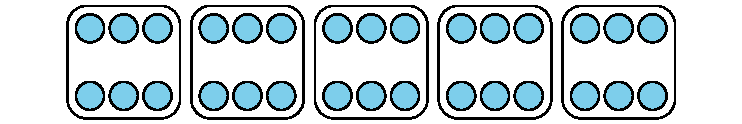
\includegraphics[width=\linewidth]{external/svg-source/tikz-file-147473.pdf}
\end{sbspanel}%
\begin{sbspanel}{0.45}%

\includegraphics[width=\linewidth]{external/svg-source/tikz-file-147472.pdf}
\end{sbspanel}%
\end{sidebyside}%
 Los estudiantes usan la relación entre multiplicación y división para afianzar su conocimiento de hechos de multiplicación y división de un solo dígito. Continúan razonando sobre productos de dos números en términos del área de rectángulos cuyas longitudes de lado representan los factores, descomponiendo longitudes de lado y aplicando propiedades de operaciones en el proceso.%
 \par
\begin{image}{0.35}{0.3}{0.35}{}%
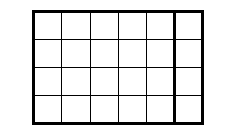
\includegraphics[width=\linewidth]{external/svg-source/tikz-file-170303.pdf}
\end{image}%
%
 \par
Hacia el final de la unidad, los estudiantes resuelven problemas de dos pasos que involucran las cuatro operaciones. En algunas situaciones, trabajan con expresiones que usan paréntesis para indicar qué operación se completa primero. Por ejemplo: \(276 + (45 \div 5) = {?}\).%
\end{abstract}
\renewcommand*{\abstractname}{Resumen}
\begin{abstract}
Este documento (HTML, pdf, latex o epub) se generó con \href{https://pretextbook.org}{PreTeXt}\footnote{\nolinkurl{pretextbook.org}\label{meta-source-2-2}}. El código fuente con el contenido para generarlo se encuentra en \href{https://github.com/enriqueacosta/IllustrativeMath-GrupoLEMA}{\nolinkurl{github.com/enriqueacosta}}.%
\end{abstract}
\renewcommand*{\abstractname}{Resumen}
\begin{abstract}
2024~Versión PreTeXt, traducciones completas de las guías y adaptaciones © Enrique Acosta (\href{https://enriqueacosta.github.io}{\nolinkurl{enriqueacosta.github.io}}). Iniciativa del Grupo LEMA (\href{https://www.grupolema.org}{\nolinkurl{www.grupolema.org}})Publicado bajo una licencia Creative Commons Attribution-NonCommercial-ShareAlike 4.0 International (CC BY SA NC 4.0).%
\par
En breve e incompleto (los detalles están en las licencias), \alert{tiene toda libertad para adaptar, copiar y distribuir este material siempre y cuando le mantenga la misma licencia, incluya la atribución correspondiente (mencione a Enrique Acosta, al Grupo LEMA, a Illustrative Mathematics y a OpenUp Resources en la forma que se describe a continuación) y lo use para fines no comerciales}.%
\par
Ver detalles de la licencia en \href{https://creativecommons.org/licenses/by-nc-sa/4.0/}{creativecommons.org}\footnote{\nolinkurl{creativecommons.org/licenses/by-nc-sa/4.0/}\label{meta-copyright-6-2}}.%
\par
Además, se permite la impresión y distribución a costo para uso educativo o personal. La reventa comercial o actividades con fines de lucro no están permitidas sin autorización previa.%
\par
Grados K-5 adaptados de IM K–5 Math v.I, ©~2021 Illustrative Mathematics~® \href{https://curriculum.illustrativemathematics.org}{illustrativemathematics.org}\footnote{\nolinkurl{curriculum.illustrativemathematics.org}\label{meta-copyright-8-4}} en su versión en español en \href{https://im.kendallhunt.com/K5_ES/curriculum.html}{im.kendallhunt.com}\footnote{\nolinkurl{im.kendallhunt.com/K5_ES/curriculum.html}\label{meta-copyright-8-6}}, distribuido con una licencia Creative Commons Attribution 4.0 International License (CC BY 4.0). Ver detalles de esta licencia en \href{https://creativecommons.org/licenses/by/4.0/}{creativecommons.org}\footnote{\nolinkurl{creativecommons.org/licenses/by/4.0/}\label{meta-copyright-8-8}}.%
\par
Grados 6-8 adaptados de IM 6–8 v3.1415, ©~2019 Illustrative Mathematics~® \href{https://curriculum.illustrativemathematics.org}{illustrativemathematics.org}\footnote{\nolinkurl{curriculum.illustrativemathematics.org}\label{meta-copyright-9-4}} en su versión en español en \href{https://im.kendallhunt.com/K5_ES/curriculum.html}{im.kendallhunt.com}\footnote{\nolinkurl{im.kendallhunt.com/K5_ES/curriculum.html}\label{meta-copyright-9-6}}, distribuido con una licencia Creative Commons Attribution 4.0 International License (CC BY 4.0), a su vez ©~2017-2019 Open Up Resources 6–8 Math v2, disponibles en \href{https://openupresources.org/math-curriculum/}{openupresources.org}\footnote{\nolinkurl{openupresources.org/math-curriculum/}\label{meta-copyright-9-9}}, con la misma licencia (CC BY 4.0). Ver detalles de esta licencia en \href{https://creativecommons.org/licenses/by/4.0/}{creativecommons.org}\footnote{\nolinkurl{creativecommons.org/licenses/by/4.0/}\label{meta-copyright-9-11}}.%
\par
\alert{Nota:} Las traducciones anteriormente mencionadas fueron lideradas y coordinadas por miembros del Grupo LEMA. Ver detalles en:%
\begin{itemize}[label=\textbullet]
\item{}K-5: \href{https://curriculum.illustrativemathematics.org/k5/teachers/grade-1/course-guide/contributors.html}{illustrativemathematics.org}\footnote{\nolinkurl{curriculum.illustrativemathematics.org/k5/teachers/grade-1/course-guide/contributors.html}\label{meta-copyright-10-2-1-2}}%
\item{}6-8: \href{https://curriculum.illustrativemathematics.org/MS/teachers/1/contributors.html}{illustrativemathematics.org}\footnote{\nolinkurl{curriculum.illustrativemathematics.org/MS/teachers/1/contributors.html}\label{meta-copyright-10-2-2-2}}%
\item{}\href{https://enriqueacosta.github.io/blog/es/posts/translating-im/}{enriqueacosta.github.io}\footnote{\nolinkurl{enriqueacosta.github.io/blog/es/posts/translating-im/}\label{meta-copyright-10-2-3-2}}%
\end{itemize}
%
\par
Este material incluye imágenes con licencias abiertas que tiene copyright de sus respectivos autores. Estas imágenes mantienen los términos de sus propias licencias de uso. Ver detalles en la sección de atribuciones de imágenes.%
\end{abstract}
\renewcommand*{\abstractname}{Resumen}
\begin{abstract}
Las siguientes personas aportaron en el desarrollo de esta versión de Matemáticas Ilustrativas.%
\par
Traducción y procesamiento de contenido%
%
\begin{itemize}[label=\textbullet]
\item{}Enrique Acosta Jaramillo%
\item{}Andrés Forero Cuervo%
\item{}Nathaly Otero Paternina%
\item{}Jonathan Defelipe Payane%
\end{itemize}
Ingeniería y desarrollo%
%
\begin{itemize}[label=\textbullet]
\item{}Enrique Acosta Jaramillo%
\end{itemize}
Autores (en inglés)%
%
\begin{itemize}[label=\textbullet]
\item{}Illustrative Mathematics. Ver detalles en los siguientes enlaces.%
%
\begin{itemize}[label=$\circ$]
\item{}K-5: \href{https://im.kendallhunt.com/k5_es/teachers/grade-4/course-guide/contributors.html}{https:\slash{}\slash{}im.kendallhunt.com\slash{}k5\slash{}}\footnote{\nolinkurl{im.kendallhunt.com/k5_es/teachers/grade-4/course-guide/contributors.html}\label{meta-contributors-8-1-2-1-2}}%
\item{}6-8: \href{https://im.kendallhunt.com/MS/teachers/2/contributors.html}{https:\slash{}\slash{}im.kendallhunt.com\slash{}MS\slash{}}\footnote{\nolinkurl{im.kendallhunt.com/MS/teachers/2/contributors.html}\label{meta-contributors-8-1-2-2-2}}%
\end{itemize}
\end{itemize}
\end{abstract}
\renewcommand*{\abstractname}{Resumen}
\begin{abstract}
Los distintos formatos de este documento (PDF, LaTeX, EPUB) se generaron utilizando software de licencia abierta desarrollado gracias al esfuerzo de muchas personas. Entre estos destacamos:%
%
\begin{itemize}[label=\textbullet]
\item{}\href{https://pretextbook.org}{Pretext}\footnote{\nolinkurl{pretextbook.org}\label{meta-attributionsOpenSource-3-1-2}}: Sistema para crear y publicar libros de texto, artículos de investigación y monografías, especialmente en disciplinas STEM.%
\item{}\href{https://www.mathjax.org}{MathJax}\footnote{\nolinkurl{www.mathjax.org}\label{meta-attributionsOpenSource-3-2-2}}: Biblioteca JavaScript para mostrar fórmulas matemáticas en cualquier navegador web.%
\item{}\href{https://www.latex-project.org}{LaTeX}\footnote{\nolinkurl{www.latex-project.org}\label{meta-attributionsOpenSource-3-3-2}} y \href{https://tug.org}{TeX}\footnote{\nolinkurl{tug.org}\label{meta-attributionsOpenSource-3-3-4}}: Sistema de preparación de documentos para impresión, ampliamente usado para documentos profesionales.%
\item{}\href{https://ctan.org/pkg/pgf}{TikZ}\footnote{\nolinkurl{ctan.org/pkg/pgf}\label{meta-attributionsOpenSource-3-4-2}}: Paquete de LaTeX para crear gráficos vectoriales de alta calidad, desde diagramas matemáticos hasta ilustraciones técnicas y científicas.%
\item{}\href{https://ctan.org/pkg/fontawesome}{FontAwesome}\footnote{\nolinkurl{ctan.org/pkg/fontawesome}\label{meta-attributionsOpenSource-3-5-2}}: Iconos vectoriales y herramientas de diseño para LaTeX.%
\end{itemize}
\end{abstract}
%
%
\typeout{************************************************}
\typeout{Sección  Sección A -~¿Qué es la división?}
\typeout{************************************************}
%
\begin{sectionptx}{Sección}{Sección A -~¿Qué es la división?}{}{Sección A -~¿Qué es la división?}{}{}{gra3-uni4-secA}
\begin{introduction}{}%
\begin{objectives}{Objetivos de aprendizaje}{gra3-uni4-secA-intro-1}
%
\begin{itemize}[label=\textbullet]
\item{}Representar y solucionar problemas del tipo “¿Cuántos grupos?” y “¿Cuántos en cada grupo?”%
\end{itemize}
\end{objectives}
Lo nuevo en esta sección es que lo estudiantes ...%
\begin{itemize}[label=\textbullet]
\item{}van a conocer la división, el término \terminology{divisor} y el símbolo \(\div\).%
\item{}van a ver que un mismo diagrama de grupos iguales o una misma expresión \(a\div b\) puede representar dos situaciones muy distintas (ver la figura).%
\end{itemize}
%
\par
En unidades anteriores los estudiantes han estado trabajando en la multiplicación como el número total dado un número de grupos iguales y en número en cada grupo. Han adquirido práctica en asociar situaciones de grupos iguales con expresiones de multiplicación \(a\times b\) y diagramas de grupos iguales. Todo esto será importante en esta sección.%
\begin{figureptx}{Figura}{La figura resume cómo distintos tipos de problemas pueden corresponder a la misma expresión de división y al mismo diagrama. En \(6\div 3\) el 3 puede ser el número de grupos, y el número de elementos en cada grupo. Los estudiantes van a trabajar con todas estas representaciones y correspondencias en esta sección.}{gra3-uni4-secA-intro-4}{}%
\begin{image}{0}{1}{0}{}%
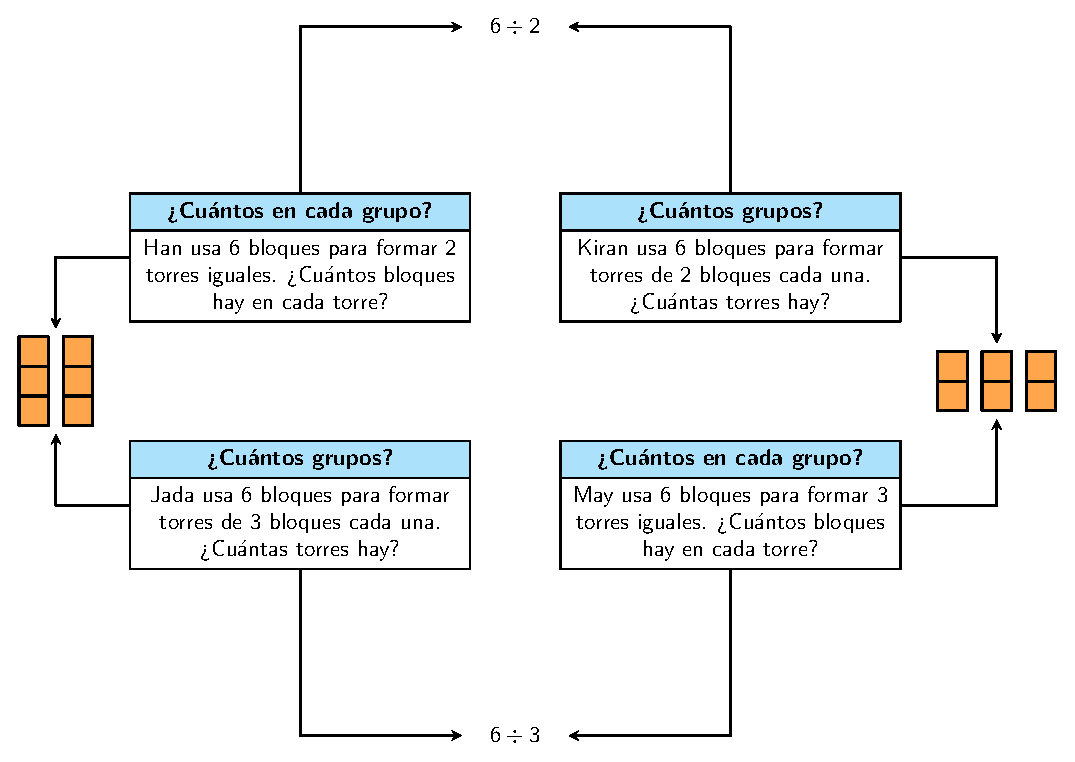
\includegraphics[width=\linewidth]{external/tikz-source/tikz-file-3-4-A-BlockDiagram.pdf}
\end{image}%
\tcblower
\end{figureptx}%
\end{introduction}%
%
%
\typeout{************************************************}
\typeout{Subsección  Lección 1 -~¿Cuántos grupos?}
\typeout{************************************************}
%
\begin{subsectionptx}{Subsección}{Lección 1 -~¿Cuántos grupos?}{}{Lección 1}{}{}{lec-cuantosGrupos}
\begin{objectives}{Objetivos de aprendizaje}{lec-cuantosGrupos-4}
%
\begin{itemize}[label=\textbullet]
\item{}Resolver problemas de "¿Cuántos grupos?" de una manera que tenga sentido para los estudiantes.%
\end{itemize}
\end{objectives}
\begin{introduction}{}%
\begin{paragraphs}{Estándares CCSS asociados.}{lec-cuantosGrupos-5-1}%
3.OA.A.2, 3.OA.A.3, 3.OA.A.3%
\end{paragraphs}%
\begin{paragraphs}{Momentos de la lección.}{lec-cuantosGrupos-5-2}%
\noindent
\begin{longtable}[l]{ll}
\addtocounter{table}{-1}
\endfirsthead
\endhead
\multicolumn{2}{r}{(Continúa en la página siguiente)}\\
\endfoot
\endlastfoot
\hyperref[lec-cuantosGrupos-warm]{Subsubsección }& Calentamiento~(10 mins)\\
\hyperref[lec-cuantosGrupos-act1]{Subsubsección }& Actividad 1~(20 mins)\\
\hyperref[lec-cuantosGrupos-act2]{Subsubsección }& Actividad 2~(15 mins)\\
\hyperref[lec-cuantosGrupos-sintesis]{Subsubsección }& Síntesis de la lección~(10 mins)\\
\hyperref[lec-cuantosGrupos-cool]{Preguntas de comprensión }& Actividad de cierre~(5 mins)\\
\end{longtable}
\end{paragraphs}%
\begin{paragraphs}{Propósito de la lección.}{lec-cuantosGrupos-5-3}%
El propósito de esta lección es que los estudiantes resuelvan problemas de "¿Cuántos grupos?" de una manera que tenga sentido para ellos.%
\end{paragraphs}%
\begin{paragraphs}{Materiales.}{lec-cuantosGrupos-5-4}%
%
\begin{itemize}[label=\textbullet]
\item{}Actividad 1%
%
\begin{itemize}[label=$\circ$]
\item{}Cubos encajables o fichas para contar%
\item{}Herramientas para crear una presentación visual%
\end{itemize}
\end{itemize}
\end{paragraphs}%
\begin{paragraphs}{Narrativa de la lección.}{lec-cuantosGrupos-5-5}%
En una unidad anterior, los estudiantes comenzaron a pensar en la idea de la multiplicación. Interpretaron los productos como el número total de objetos en una colección de grupos de igual tamaño. Los estudiantes representaron grupos de igual tamaño usando dibujos, diagramas de cinta y arreglos.%
\par
El propósito de esta lección es introducir problemas que involucren poner objetos en grupos de igual tamaño, comenzando con problemas de "¿cuántos grupos?". Aunque la estructura de los problemas sugiere división, los estudiantes pueden usar su comprensión de la multiplicación o cualquier estrategia que tenga sentido para ellos para resolverlos. Si los estudiantes usan cubos encajables, invítelos a dibujar una imagen que coincida con su trabajo. En la síntesis de la lección, los estudiantes tienen la oportunidad de pensar en cómo definir la división. Sin embargo, la definición y el símbolo de la división se presentarán en lecciones posteriores.%
\end{paragraphs}%
\begin{paragraphs}{Preguntas de reflexión.}{lec-cuantosGrupos-5-6}%
En esta lección, los estudiantes pensarán en la idea de la división por primera vez. ¿Cómo está influyendo y apoyando su comprensión de la multiplicación en la forma en que resuelven problemas de división?%
\end{paragraphs}%
\end{introduction}%
%
%
\typeout{************************************************}
\typeout{Subsubsección  Calentamiento~(10 mins)}
\typeout{************************************************}
%
\begin{subsubsectionptx}{Subsubsección}{Calentamiento~(10 mins)}{}{Calentamiento}{}{}{lec-cuantosGrupos-warm}
\par
\begin{paragraphs}{Tiempo recomendado.}{warm-cuantosVes-Manzanas-4-1}%
10 minutos.%
\end{paragraphs}%
\begin{paragraphs}{Narrativa.}{warm-cuantosVes-Manzanas-4-2}%
El propósito de este "¿Cuántos ves?" es que los estudiantes subiticen (es decir, reconozcan una cantidad de objetos sin contarlos) o utilicen estrategias de agrupamiento para describir las imágenes que ven.%
\end{paragraphs}%
\begin{paragraphs}{Lanzamiento.}{warm-cuantosVes-Manzanas-4-3}%
%
\begin{itemize}[label=\textbullet]
\item{}Grupos de 2%
\item{}``¿Cuántas ven? ¿Cómo lo saben?, ¿qué ven?''%
\item{}Muestre rápidamente la imagen (3 segundos).%
\item{}30 segundos: tiempo de reflexión en silencio%
\end{itemize}
\end{paragraphs}%
\begin{paragraphs}{Desarrollo de la actividad.}{warm-cuantosVes-Manzanas-4-4}%
%
\begin{itemize}[label=\textbullet]
\item{}Muestre nuevamente la imagen.%
\item{}``Discutan con su compañero cómo pensaron''%
\item{}1 minuto: discusión con el compañero%
\item{}Registre las respuestas.%
\end{itemize}
\end{paragraphs}%
\begin{exploration}{Calentamiento}{Cuántos ves: Manzanas.}{warm-cuantosVes-Manzanas}%
¿Cuántas ves?\\
 ¿Cómo lo sabes?, ¿qué ves?%
\begin{image}{0}{1}{0}{}%
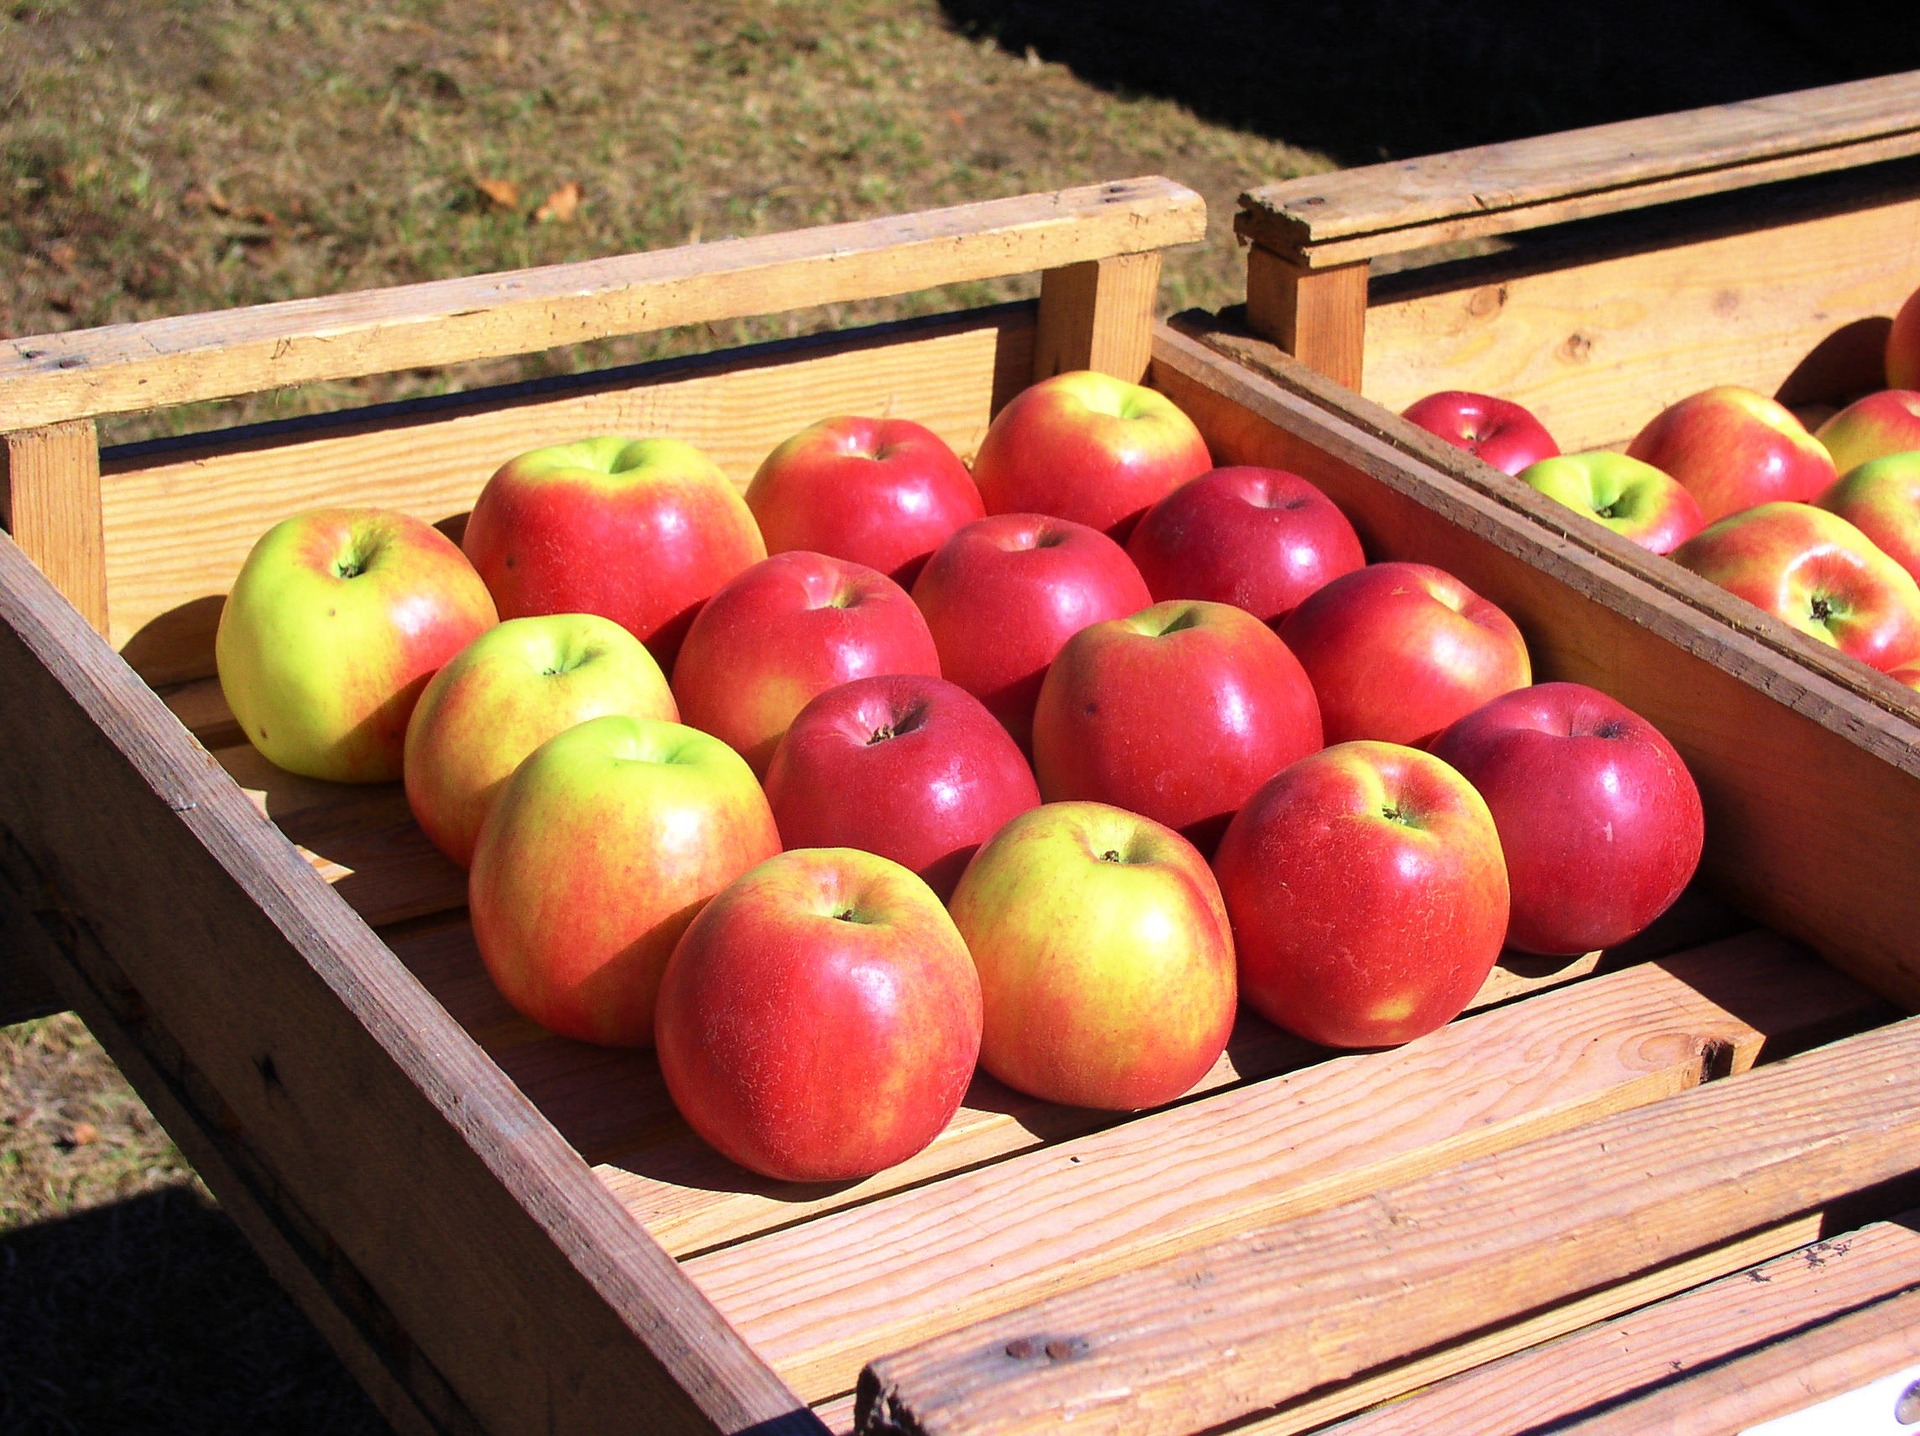
\includegraphics[width=\linewidth]{external/jpg-source/apples-1642732_1920.jpg}
\end{image}%
\par\smallskip%
\noindent\textbf{\blocktitlefont Solución}.\hypertarget{warm-cuantosVes-Manzanas-3}{}\quad{}Ejemplos de respuestas:%
%
\begin{itemize}[label=\textbullet]
\item{}16 porque veo 4 filas (o columnas) de 4.%
\item{}16 porque veo 2 grupos de 8 manzanas, entonces multipliqué \(8\times 2\)%
\item{}23 porque veo 4 grupos de 4 en una caja y 7 manzanas más en la otra caja, lo que da 23.%
\end{itemize}
\end{exploration}%
\footnotetext[21]{\nolinkurl{pixabay.com/photos/apples-fruit-apple-1642732/}\label{warm-cuantosVes-Manzanas-2-2-2-1-2}}%
\par
\begin{paragraphs}{Síntesis de la actividad.}{warm-cuantosVes-Manzanas-5-1}%
%
\begin{itemize}[label=\textbullet]
\item{}``¿Cómo los ayudó la forma en la que estaban organizadas las manzanas a ver cuántas había?'' (Vi 2 filas de 4 y supe que eran 8 manzanas, luego dupliqué eso para encontrar cuántas manzanas había en la caja. Vi grupos de 4, así que multipliqué \(4\times 4\) y luego sumé las otras manzanas.)%
\item{}Considera preguntar:%
\begin{itemize}[label=$\circ$]
\item{}``¿Alguien puede expresar con otras palabras la forma en la que \fillintext{10} vio las manzanas?''%
\item{}``¿Alguien vio las manzanas de la misma forma, pero lo explicaría de otra manera?''%
\item{}``¿Alguien quiere compartir otra observación sobre la forma en la que \fillintext{10} vio las manzanas?''%
\end{itemize}
%
\end{itemize}
\end{paragraphs}%
\end{subsubsectionptx}
%
%
\typeout{************************************************}
\typeout{Subsubsección  Actividad 1~(20 mins)}
\typeout{************************************************}
%
\begin{subsubsectionptx}{Subsubsección}{Actividad 1~(20 mins)}{}{Actividad 1}{}{}{lec-cuantosGrupos-act1}
\par
\begin{paragraphs}{Tiempo recomendado.}{act-cuantasManzanas-4-1}%
20 minutos.%
\end{paragraphs}%
\begin{paragraphs}{Narrativa.}{act-cuantasManzanas-4-2}%
El propósito de esta actividad es que los estudiantes representen y resuelvan problemas de "¿cuántos grupos?". Invítelos a utilizar cualquier estrategia y representación visual que les parezca lógica.%
\par
Los estudiantes crean un póster de su solución al primer problema con un compañero. En la siguiente actividad, los estudiantes participan en un recorrido por el salón para observar los pósters.%
\par
Identifique a los estudiantes que representen la situación con:%
%
\begin{itemize}[label=\textbullet]
\item{}objetos concretos: colocando 24 cubos en grupos de 8%
\item{}dibujos de objetos: dibujando 24 manzanas y luego separándolas en grupos de 8 o rodeando grupos de 8%
\item{}arreglos: dibujando 3 filas de 8 manzanas cada una para llegar a 24%
\end{itemize}
Cuando los estudiantes representan la situación con objetos, dibujos concretos o dibujos abstractos, están razonando de manera abstracta y cuantitativa (MP2).%
\end{paragraphs}%
\begin{paragraphs}{Materiales.}{act-cuantasManzanas-4-3}%
%
\begin{itemize}[label=\textbullet]
\item{}Cubos encajables o fichas para contar%
\item{}Herramientas para crear una presentación visual%
\end{itemize}
\end{paragraphs}%
\begin{paragraphs}{Lanzamiento.}{act-cuantasManzanas-4-4}%
%
\begin{itemize}[label=\textbullet]
\item{}Grupos de 2%
\item{}Dele a los estudiantes acceso a cubos encajables o fichas para contar.%
\end{itemize}
\end{paragraphs}%
\begin{paragraphs}{Desarrollo de la actividad.}{act-cuantasManzanas-4-5}%
%
\begin{itemize}[label=\textbullet]
\item{}``Resuelvan estos problemas. Usen objetos, un dibujo o un diagrama para mostrar cómo pensaron.''%
\item{}6-8 minutos: tiempo de trabajo independiente%
\item{}Mientras los estudiantes trabajan, considere preguntar:%
\begin{itemize}[label=$\circ$]
\item{}``¿Cómo pueden representar lo que están pensando?''%
\item{}``¿En qué parte de su trabajo podemos ver las manzanas?''%
\item{}``¿En qué parte de su trabajo podemos ver cuántas cajas hay?''%
\end{itemize}
%
\item{}Identifique a los estudiantes que resuelvan el primer problema de la misma manera. Organícelos en grupos de 2 para que creen un póster juntos.%
\item{}``Ahora van a hacer un póster para mostrar cómo pensaron en el primer problema''%
\item{}``Van a trabajar con un compañero que haya resuelto el problema de la misma forma que ustedes''%
\item{}Proporcione a cada grupo herramientas para hacer una exhibición visual.%
\item{}6-8 minutos: tiempo de trabajo en pareja%
\end{itemize}
\end{paragraphs}%
\begin{activity}{Actividad}{¿Cuántas manzanas?}{act-cuantasManzanas}%
Resuelve cada problema. Muestra cómo pensaste. Usa objetos, un dibujo o un diagrama.%
\par
%
\begin{enumerate}
\item{}Si 24 manzanas se ponen en cajas y en cada caja se ponen 8 manzanas, ¿cuántas cajas hay?%
\item{}Si 42 manzanas se ponen en cajas y en cada caja se ponen 6 manzanas, ¿cuántas cajas hay?%
\item{}Si 32 manzanas se ponen en cajas y en cada caja se ponen 4 manzanas, ¿cuántas cajas hay?%
\end{enumerate}
%
\par\smallskip%
\noindent\textbf{\blocktitlefont Solución}.\hypertarget{act-cuantasManzanas-3}{}\quad{}Ejemplos de respuestas:%
%
\begin{enumerate}
\item{}3 cajas. Ejemplo de razonamiento: Los estudiantes dibujan 8 manzanas en cada fila y observan que hay 3 filas.%
\item{}7 cajas. Ejemplo de razonamiento: Los estudiantes dibujan 42 manzanas y marcan grupos de 6 hasta que no quedan manzanas.%
\item{}8 cajas. Ejemplo de razonamiento: Los estudiantes toman 32 cubos y arman grupos de 4 para representar cada caja.%
\end{enumerate}
\end{activity}%
\par
\begin{paragraphs}{Para los estudiantes con dificultades.}{act-cuantasManzanas-5-1}%
Si los estudiantes no encuentran una solución a los problemas, considere preguntar: "¿De qué se trata este problema?" y "¿Cómo podrías representar el problema?"%
\end{paragraphs}%
\begin{paragraphs}{Síntesis de la actividad.}{act-cuantasManzanas-5-2}%
Organice los pósteres alrededor del salón.%
\end{paragraphs}%
\begin{paragraphs}{Acceso a estudiantes con discapacidades.}{act-cuantasManzanas-5-3}%
Representación: Acceso para la percepción.%
\par
Comience mostrando cómo podría verse el póster, utilizando un problema diferente, para apoyar la comprensión del contexto.%
\par
Apoya la accesibilidad para: Funcionamiento socioemocional%
\end{paragraphs}%
\end{subsubsectionptx}
%
%
\typeout{************************************************}
\typeout{Subsubsección  Actividad 2~(15 mins)}
\typeout{************************************************}
%
\begin{subsubsectionptx}{Subsubsección}{Actividad 2~(15 mins)}{}{Actividad 2}{}{}{lec-cuantosGrupos-act2}
\par
\begin{paragraphs}{Tiempo recomendado.}{act-recorridoSalon-manzanasEnCajas-4-1}%
15 minutos.%
\end{paragraphs}%
\begin{paragraphs}{Narrativa.}{act-recorridoSalon-manzanasEnCajas-4-2}%
El propósito de esta actividad es que los estudiantes consideren en qué se parecen y en qué se diferencian las formas en las que resolvieron un problema de "¿cuántos grupos?" en la actividad anterior.%
\par
A medida que los estudiantes visiten los pósters, identifique de 2 a 3 estudiantes que demuestren especialmente bien que este problema se trata de encontrar cuántos grupos se forman. Selecciónelos para compartir sus explicaciones en la próxima lección.%
\end{paragraphs}%
\begin{paragraphs}{Lanzamiento.}{act-recorridoSalon-manzanasEnCajas-4-3}%
Estudiantes en parejas.\end{paragraphs}%
\begin{paragraphs}{Desarrollo de la actividad.}{act-recorridoSalon-manzanasEnCajas-4-4}%
%
\begin{itemize}[label=\textbullet]
\item{}``Cuando vayan a ver los pósteres con su compañero, discutan en qué se parecen y en qué se diferencian las ideas que se muestran en los pósteres''%
\item{}8–10 minutos: Recorrido por el salón.%
\end{itemize}
\end{paragraphs}%
\begin{activity}{Actividad}{Recorrido por el salón: Manzanas en cajas.}{act-recorridoSalon-manzanasEnCajas}%
%
\begin{enumerate}
\item{}Con tu compañero, ve a ver los pósteres alrededor del salón. Discute con tu compañero en qué se parecen y en qué se diferencian las ideas que se muestran en los pósteres.%
\item{}Reflexiona sobre lo que viste. Escribe una cosa en la que se parecen y una cosa en la que se diferencian las ideas que se muestran en los pósteres.%
\end{enumerate}
%
\par\smallskip%
\noindent\textbf{\blocktitlefont Solución}.\hypertarget{act-recorridoSalon-manzanasEnCajas-3}{}\quad{}%
\begin{enumerate}
\item{}(sin respuestas)%
\item{}Ejemplos de respuestas:%
\begin{itemize}[label=\textbullet]
\item{}En cada póster, la idea es poner 24 manzanas en cajas que tengan 8 manzanas.%
\item{}Al final, siempre hay 3 cajas.%
\item{}En algunos pósteres, podemos ver cómo se ponen las manzanas en cada grupo. En otros pósteres, solo podemos ver el resultado final.%
\end{itemize}
%
\end{enumerate}
\end{activity}%
\par
\begin{paragraphs}{Síntesis de la actividad.}{act-recorridoSalon-manzanasEnCajas-5-1}%
%
\begin{itemize}[label=\textbullet]
\item{}Brinde a los estudiantes la oportunidad de hacer preguntas sobre cualquier póster.%
\item{}``¿En qué se parecen las ideas que se muestran en los pósteres?''%
\item{}``¿En qué se diferencian las ideas que se muestran en los pósteres?''%
\end{itemize}
\end{paragraphs}%
\begin{paragraphs}{Desarrollo de lenguaje matemático.}{act-recorridoSalon-manzanasEnCajas-5-2}%
Apoyos para la discusión de MLR8:%
\par
Muestre esquema de oraciones para apoyar la escritura de los estudiantes: ``Una cosa que observé que es parecida es...'', ``Una cosa que observé que es diferente es...'', ``Una cosa en la que se parecen es...'', ``Una diferencia es...''.%
\par
Avances: Escritura, Habla%
\end{paragraphs}%
\end{subsubsectionptx}
%
%
\typeout{************************************************}
\typeout{Subsubsección  Síntesis de la lección~(10 mins)}
\typeout{************************************************}
%
\begin{subsubsectionptx}{Subsubsección}{Síntesis de la lección~(10 mins)}{}{Síntesis de la lección}{}{}{lec-cuantosGrupos-sintesis}
Tiempo recomendado: 10 mins.%
\par
``Hoy resolvimos problemas acerca de poner manzanas en cajas. ¿En qué se parecían estos problemas a los problemas de multiplicación? ¿En qué eran diferentes?'' (Estos problemas tenían grupos de igual tamaño. En la multiplicación contamos cuántas cosas había en total. En estos problemas ya lo sabíamos. Queríamos encontrar cuántos grupos podíamos hacer).%
\par
``Los problemas que resolvimos hoy son problemas de división. ¿Cómo definirían la división basándose en los problemas que vimos hoy?'' (La división se trata de poner en grupos de igual tamaño. Yo diría que se trata de encontrar cuántos grupos puedes hacer).%
\end{subsubsectionptx}
%
%
\typeout{************************************************}
\typeout{Preguntas de comprensión  Actividad de cierre~(5 mins)}
\typeout{************************************************}
%
\begin{reading-questions-subsubsection}{Preguntas de comprensión}{Actividad de cierre~(5 mins)}{}{Actividad de cierre}{}{}{lec-cuantosGrupos-cool}
\href{external/cools-pdf/cool-cuantasBolsas-standalone.pdf}{Descargar pdf para imprimir o proyectar}\footnote{\nolinkurl{external/cools-pdf/cool-cuantasBolsas-standalone.pdf}\label{lec-cuantosGrupos-cool-5}}\begin{project}{Actividad de cierre}{¿Cuántas bolsas?}{cool-cuantasBolsas}%
Lin tiene 30 manzanas para compartir con sus amigos. Las pone en bolsas y pone 6 manzanas en cada bolsa. ¿Cuántas bolsas necesita? Explica o muestra tu razonamiento.%
\par\smallskip%
\noindent\textbf{\blocktitlefont Solución}.\hypertarget{cool-cuantasBolsas-3}{}\quad{}Necesitará 5 bolsas. Si pone las 30 manzanas en grupos de 6, habrá 5 grupos.%
\begin{image}{0}{1}{0}{}%
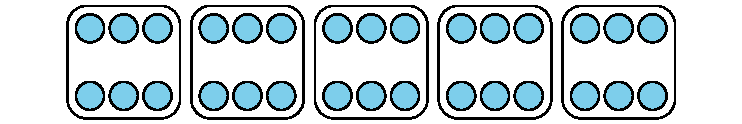
\includegraphics[width=\linewidth]{external/svg-source/tikz-file-147473.pdf}
\end{image}%
\end{project}%
\par
\begin{paragraphs}{Posibles errores.}{cool-cuantasBolsas-4-1}%
Los estudiantes representan 6 bolsas de manzanas en lugar de 6 manzanas en cada bolsa.%
\end{paragraphs}%
\begin{paragraphs}{Acciones para apoyar el aprendizaje.}{cool-cuantasBolsas-4-2}%
Reparta al inicio de la siguiente lección las respuestas de los estudiantes, y pida que trabajen en parejas en este problema.%
\end{paragraphs}%
\end{reading-questions-subsubsection}
\end{subsectionptx}
%
%
\typeout{************************************************}
\typeout{Subsección  Lección 2 -~¿Cuántos hay en cada grupo?}
\typeout{************************************************}
%
\begin{subsectionptx}{Subsección}{Lección 2 -~¿Cuántos hay en cada grupo?}{}{Lección 2}{}{}{lec-cuantosEnCadaGrupo}
\begin{objectives}{Objetivos de aprendizaje}{lec-cuantosEnCadaGrupo-4}
%
\begin{itemize}[label=\textbullet]
\item{}Solucionar problemas de “¿cuántos hay en cada grupo?” usando alguna estrategia que tenga sentido para los estudiantes.%
\end{itemize}
\end{objectives}
\begin{introduction}{}%
\begin{paragraphs}{Estándares CCSS asociados.}{lec-cuantosEnCadaGrupo-5-1}%
3.OA.A.2, 3.OA.A.3, 3.OA.A.3%
\end{paragraphs}%
\begin{paragraphs}{Momentos de la lección.}{lec-cuantosEnCadaGrupo-5-2}%
\noindent
\begin{longtable}[l]{ll}
\addtocounter{table}{-1}
\endfirsthead
\endhead
\multicolumn{2}{r}{(Continúa en la página siguiente)}\\
\endfoot
\endlastfoot
\hyperref[lec-cuantosEnCadaGrupo-warm]{Subsubsección }& Calentamiento~(10 mins)\\
\hyperref[lec-cuantosEnCadaGrupo-act1]{Subsubsección }& Actividad 1~(15 mins)\\
\hyperref[lec-cuantosEnCadaGrupo-act2]{Subsubsección }& Actividad 2~(10 mins)\\
\hyperref[lec-cuantosEnCadaGrupo-act3]{Subsubsección }& Actividad 3~(10 mins)\\
\hyperref[lec-cuantosEnCadaGrupo-sintesis]{Subsubsección }& Síntesis de la lección~(10 mins)\\
\hyperref[lec-cuantosEnCadaGrupo-cool]{Preguntas de comprensión }& Actividad de cierre~(5 mins)\\
\end{longtable}
\end{paragraphs}%
\begin{paragraphs}{Propósito de la lección.}{lec-cuantosEnCadaGrupo-5-3}%
El propósito de esta lección es que los estudiantes resuelvan problemas de "¿cuántos en cada grupo?" de una manera que tenga sentido para ellos.%
\end{paragraphs}%
\begin{paragraphs}{Materiales.}{lec-cuantosEnCadaGrupo-5-4}%
%
\begin{itemize}[label=\textbullet]
\item{}Actividad 1%
%
\begin{itemize}[label=$\circ$]
\item{}Cubos encajables o fichas de dos colores%
\item{}Herramientas para crear una presentación visual%
\end{itemize}
\end{itemize}
\end{paragraphs}%
\begin{paragraphs}{Narrativa de la lección.}{lec-cuantosEnCadaGrupo-5-5}%
Previamente, los estudiantes resolvieron problemas de "¿cuántos grupos?" de una manera que tenía sentido para ellos. En esta lección, los estudiantes trabajan con problemas más amplios que involucran repartir en grupos de igual tamaño e incluyen problemas de "¿cuántos en cada grupo?". Nuevamente en esta lección los estudiantes tienen la flexibilidad de representar y resolver problemas utilizando cualquier estrategia que tenga sentido para ellos. Si los estudiantes usan cubos encajables, invítelos a dibujar una imagen que coincida con su trabajo. Al final de esta lección, la división se define como encontrar el número de grupos o encontrar el tamaño de cada grupo cuando repartimos en grupos de igual tamaño.%
\end{paragraphs}%
\begin{paragraphs}{Preguntas de reflexión.}{lec-cuantosEnCadaGrupo-5-6}%
¿Qué dije, hice o pregunté durante la síntesis de la lección que ayudó a los estudiantes a tener claridad sobre el aprendizaje del día? ¿Haber entendido la actividad de cierre antes de enseñar hoy tuvo algún beneficio a la hora de sintetizar el aprendizaje de la lección? ¿Cómo?%
\end{paragraphs}%
\end{introduction}%
%
%
\typeout{************************************************}
\typeout{Subsubsección  Calentamiento~(10 mins)}
\typeout{************************************************}
%
\begin{subsubsectionptx}{Subsubsección}{Calentamiento~(10 mins)}{}{Calentamiento}{}{}{lec-cuantosEnCadaGrupo-warm}
\par
\begin{paragraphs}{Tiempo recomendado.}{warm-observa-arbolManzanas-4-1}%
10 minutos%
\end{paragraphs}%
\begin{paragraphs}{Narrativa.}{warm-observa-arbolManzanas-4-2}%
El propósito de esta actividad de calentamiento es generar la idea de que se pueden hacer muchas preguntas diferentes sobre una situación, lo cual será útil cuando los estudiantes resuelvan problemas en una actividad posterior.%
\end{paragraphs}%
\begin{paragraphs}{Lanzamiento.}{warm-observa-arbolManzanas-4-3}%
%
\begin{itemize}[label=\textbullet]
\item{}Grupos de 2%
\item{}Muestre la imagen.%
\item{}``¿Qué observan? ¿Qué se preguntan?''%
\item{}1 minuto: tiempo de reflexión en silencio%
\end{itemize}
\end{paragraphs}%
\begin{paragraphs}{Desarrollo de la actividad.}{warm-observa-arbolManzanas-4-4}%
%
\begin{itemize}[label=\textbullet]
\item{}``Discutan con su compañero lo que pensaron''%
\item{}1 minuto: discusión con el compañero%
\item{}Compartan y registren las respuestas.%
\end{itemize}
\end{paragraphs}%
\begin{exploration}{Calentamiento}{Observa y pregúntate: Más manzanas.}{warm-observa-arbolManzanas}%
¿Qué observas?\\
 ¿Qué te preguntas?%
\begin{image}{0.15}{0.7}{0.15}{}%
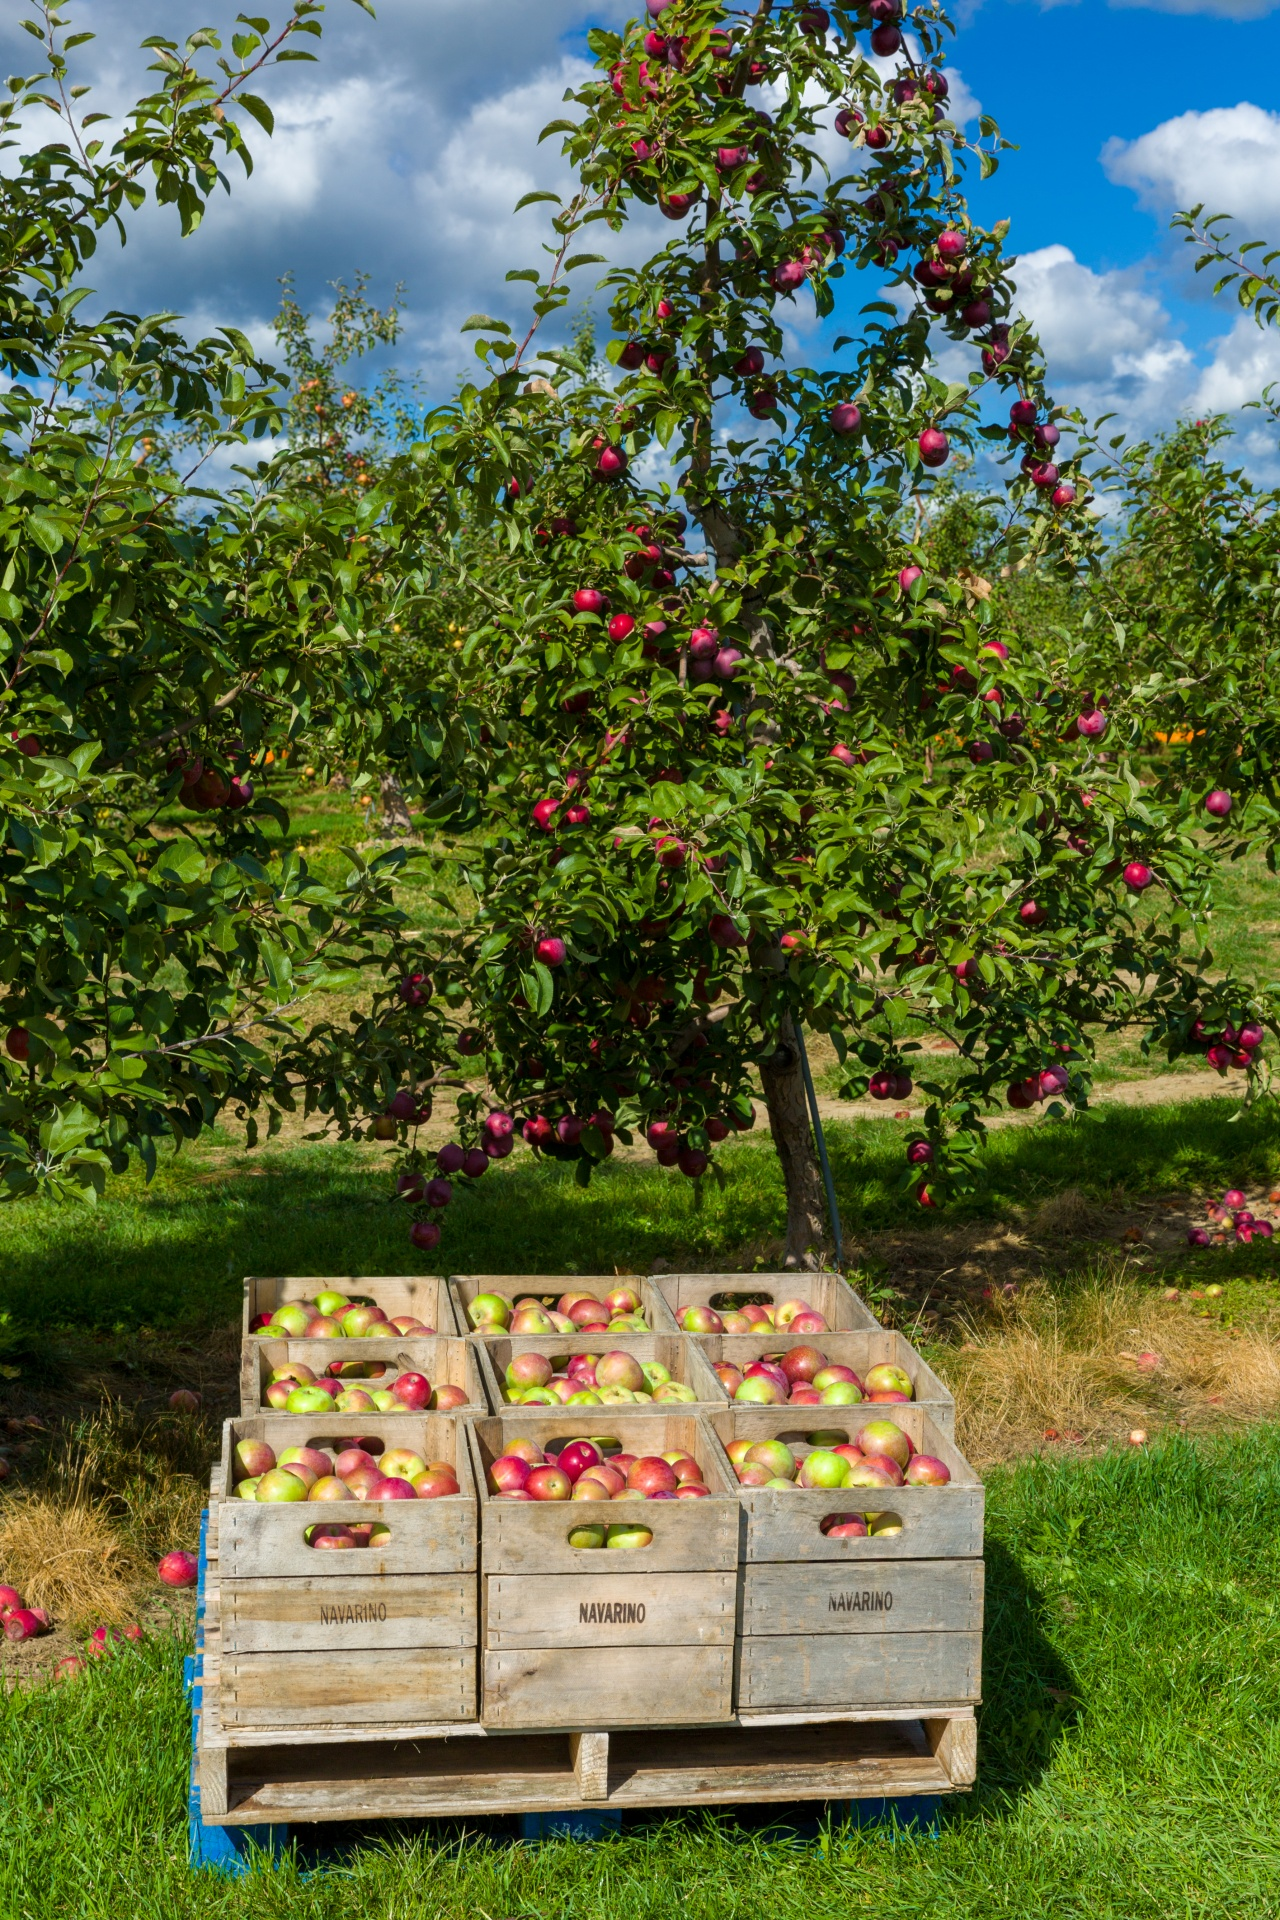
\includegraphics[width=\linewidth]{external/jpg-source/3.4.A2 Warm-up.jpg}
\end{image}%
\par\smallskip%
\noindent\textbf{\blocktitlefont Solución}.\hypertarget{warm-observa-arbolManzanas-3}{}\quad{}Los estudiantes pueden observar:%
\begin{itemize}[label=\textbullet]
\item{}Algunas manzanas están en cajas.%
\item{}Algunas manzanas todavía están en el árbol.%
\item{}Hay 9 cajas de manzanas.%
\end{itemize}
%
\par
Los estudiantes pueden preguntarse:%
\begin{itemize}[label=\textbullet]
\item{}¿Cómo se metieron las manzanas en las cajas?%
\item{}¿Cuántas manzanas hay en las cajas?%
\item{}¿Cada caja tiene el mismo número de manzanas?%
\end{itemize}
%
\end{exploration}%
\footnotetext[23]{\nolinkurl{www.publicdomainpictures.net/en/view-image.php?image=267667\&picture=apple-orchard}\label{warm-observa-arbolManzanas-2-2-2-1-2}}%
\par
\begin{paragraphs}{Síntesis de la actividad.}{warm-observa-arbolManzanas-5-1}%
Si no se menciona en las respuestas de los estudiantes, pregunte: "¿Qué preguntas matemáticas podemos hacer sobre esta imagen?" (¿Cuántas manzanas hay en cada caja? ¿Hay más manzanas en las cajas que en los árboles? ¿Cuántas manzanas hay en total en las cajas?)%
\end{paragraphs}%
\end{subsubsectionptx}
%
%
\typeout{************************************************}
\typeout{Subsubsección  Actividad 1~(15 mins)}
\typeout{************************************************}
%
\begin{subsubsectionptx}{Subsubsección}{Actividad 1~(15 mins)}{}{Actividad 1}{}{}{lec-cuantosEnCadaGrupo-act1}
\par
\begin{paragraphs}{Tiempo recomendado.}{act-cuantasManzanas2-4-1}%
15 minutos%
\end{paragraphs}%
\begin{paragraphs}{Narrativa.}{act-cuantasManzanas2-4-2}%
El propósito de esta actividad es que los estudiantes representen y resuelvan problemas de "¿cuántos en cada grupo?" utilizando la estrategia y representación visual que les parezca más lógica. Los estudiantes crean un póster de su solución al primer problema con un compañero. En la siguiente actividad, participan en un recorrido por el salón para observar los pósteres.%
\par
Identifique a los estudiantes que representen la situación con:%
%
\begin{itemize}[label=\textbullet]
\item{}Objetos concretos: colocando 20 cubos en 4 grupos uno por uno.%
\item{}Dibujos de objetos: dibujando 20 manzanas y luego separándolas en 4 grupos.%
\item{}Arreglos: dibujando 4 filas con una manzana en cada fila y así sucesivamente hasta llegar a 20.%
\end{itemize}
\end{paragraphs}%
\begin{paragraphs}{Materiales.}{act-cuantasManzanas2-4-3}%
%
\begin{itemize}[label=\textbullet]
\item{}Cubos encajables o fichas de dos colores%
\item{}Herramientas para crear una presentación visual%
\end{itemize}
\end{paragraphs}%
\begin{paragraphs}{Lanzamiento.}{act-cuantasManzanas2-4-4}%
%
\begin{itemize}[label=\textbullet]
\item{}Grupos de 2%
\item{}Proporcione a los estudiantes acceso a cubos encajables y fichas.%
\item{}``Hablen con su compañero sobre cómo podrían resolver estos problemas''%
\item{}1-2 minutos: discusión en parejas%
\end{itemize}
\end{paragraphs}%
\begin{paragraphs}{Desarrollo de la actividad.}{act-cuantasManzanas2-4-5}%
%
\begin{itemize}[label=\textbullet]
\item{}``Resuelvan estos problemas. Usen objetos, un dibujo o un diagrama para mostrar cómo pensaron.''%
\item{}5-7 minutos: tiempo de trabajo independiente%
\item{}Mientras los estudiantes trabajan, considere preguntar:%
\begin{itemize}[label=$\circ$]
\item{}``¿Cómo pueden representar lo que están pensando?''%
\item{}``¿En qué parte de su trabajo pueden ver las cajas?''%
\item{}``¿En qué parte de su trabajo pueden ver cuántas manzanas hay en cada caja?''%
\end{itemize}
%
\item{}Identifique a los estudiantes que resuelven el primer problema de la misma manera. Organícelos en grupos de 2 para que creen un póster juntos.%
\item{}``Ahora van a hacer un póster para mostrar cómo pensaron en el primer problema''%
\item{}``Van a trabajar con un compañero que haya resuelto el problema de la misma forma que ustedes''%
\item{}Proporcione a cada grupo herramientas para crear una presentación visual.%
\item{}5-7 minutos: tiempo de trabajo en pareja%
\end{itemize}
\end{paragraphs}%
\begin{activity}{Actividad}{¿Cuántas manzanas?}{act-cuantasManzanas2}%
Resuelve cada problema. Muestra cómo pensaste. Usa objetos, un dibujo o un diagrama.%
\par
%
\begin{enumerate}
\item{}Si 20 manzanas se empacan en 4 cajas y en cada caja hay el mismo número de manzanas, ¿cuántas manzanas hay en cada caja?%
\item{}Si 36 manzanas se empacan en 6 cajas y en cada caja hay el mismo número de manzanas, ¿cuántas manzanas hay en cada caja?%
\item{}Si 45 manzanas se empacan en 9 cajas y en cada caja hay el mismo número de manzanas, ¿cuántas manzanas hay en cada caja?%
\end{enumerate}
%
\par\smallskip%
\noindent\textbf{\blocktitlefont Solución}.\hypertarget{act-cuantasManzanas2-3}{}\quad{}%
\begin{enumerate}
\item{}5 manzanas. Ejemplo de razonamiento: Los estudiantes dibujan las manzanas una por una en 4 filas y descubren que al final hay 5 manzanas en cada fila.%
\item{}6 manzanas. Ejemplo de razonamiento: Los estudiantes dibujan 36 manzanas y piensan en cómo separarlas en 6 grupos del mismo tamaño. Luego, marcan 6 grupos de 6.%
\item{}5 manzanas. Ejemplo de razonamiento: Los estudiantes toma 45 cubos y los ponen 1 por 1 en 9 grupos para representar cada caja.%
\end{enumerate}
\end{activity}%
\par
\begin{paragraphs}{Para los estudiantes con dificultades.}{act-cuantasManzanas2-5-1}%
Si los estudiantes no encuentran una solución a los problemas, considere preguntar: "¿De qué se trata este problema?" y "¿Cómo podrías representar el problema?"%
\end{paragraphs}%
\begin{paragraphs}{Síntesis de la actividad.}{act-cuantasManzanas2-5-2}%
Organice los pósteres alrededor del salón.%
\end{paragraphs}%
\begin{paragraphs}{Acceso a estudiantes con discapacidades.}{act-cuantasManzanas2-5-3}%
Compromiso: Desarrollar Esfuerzo y Persistencia.%
\par
Divida esta tarea en partes más manejables. Apoye a los estudiantes y bríndeles retroalimentación y motivación después de cada parte (problema).%
\par
Apoya la accesibilidad para: Atención%
\end{paragraphs}%
\end{subsubsectionptx}
%
%
\typeout{************************************************}
\typeout{Subsubsección  Actividad 2~(10 mins)}
\typeout{************************************************}
%
\begin{subsubsectionptx}{Subsubsección}{Actividad 2~(10 mins)}{}{Actividad 2}{}{}{lec-cuantosEnCadaGrupo-act2}
\par
\begin{paragraphs}{Tiempo recomendado.}{act-recorridoSalon-Manzanas2-4-1}%
10 minutos%
\end{paragraphs}%
\begin{paragraphs}{Narrativa.}{act-recorridoSalon-Manzanas2-4-2}%
El propósito de esta actividad es que los estudiantes consideren en qué se parecen y en qué se diferencian las formas en las que resolvieron un problema de "¿cuántos en cada grupo?" en la actividad anterior. A medida que los estudiantes observan los pósteres, identifique de 2 a 3 estudiantes que demuestren de manera especialmente clara que este problema se trata de encontrar cuántos hay en cada grupo. Selecciónelos para que compartan su trabajo en la próxima actividad.%
\end{paragraphs}%
\begin{paragraphs}{Lanzamiento.}{act-recorridoSalon-Manzanas2-4-3}%
Grupos de 2%
\end{paragraphs}%
\begin{paragraphs}{Desarrollo de la actividad.}{act-recorridoSalon-Manzanas2-4-4}%
%
\begin{itemize}[label=\textbullet]
\item{}``Cuando estén viendo los pósteres con su compañero, discutan en qué se parecen y en qué se diferencian las ideas que se muestran en los pósteres''%
\item{}5-7 minutos: Recorrido por el salón%
\end{itemize}
\end{paragraphs}%
\begin{activity}{Actividad}{Recorrido por el salón.}{act-recorridoSalon-Manzanas2}%
Con tu compañero, ve a ver los pósteres alrededor del salón. Discute con tu compañero en qué se parecen y en qué se diferencian las ideas que se muestran en los pósteres.%
\par\smallskip%
\noindent\textbf{\blocktitlefont Solución}.\hypertarget{act-recorridoSalon-Manzanas2-3}{}\quad{}Ejemplos de respuestas:%
%
\begin{itemize}[label=\textbullet]
\item{}En cada póster, la idea es poner 20 manzanas en 4 grupos.%
\item{}En todos los casos, hay 5 manzanas en cada caja.%
\item{}En algunos pósteres, podemos ver cómo se ponen las manzanas en cada grupo. En otros pósteres, solo podemos ver el resultado final.%
\end{itemize}
\end{activity}%
\par
\begin{paragraphs}{Síntesis de la actividad.}{act-recorridoSalon-Manzanas2-5-1}%
%
\begin{itemize}[label=\textbullet]
\item{}Brinde a los estudiantes la oportunidad de hacer preguntas sobre cualquier póster.%
\item{}``¿En qué se parecen las ideas que se muestran en los pósteres?''%
\item{}``¿En qué se diferencian las ideas que se muestran en los pósteres?''%
\end{itemize}
\end{paragraphs}%
\end{subsubsectionptx}
%
%
\typeout{************************************************}
\typeout{Subsubsección  Actividad 3~(10 mins)}
\typeout{************************************************}
%
\begin{subsubsectionptx}{Subsubsección}{Actividad 3~(10 mins)}{}{Actividad 3}{}{}{lec-cuantosEnCadaGrupo-act3}
\par
\begin{paragraphs}{Tiempo recomendado.}{act-todasLasManzanas-4-1}%
10 minutos.%
\end{paragraphs}%
\begin{paragraphs}{Narrativa.}{act-todasLasManzanas-4-2}%
El propósito de esta actividad es que los estudiantes consideren en qué se parecen y en qué son diferentes los problemas de "¿cuántos grupos?" y "¿cuántos en cada grupo?" que resolvieron en una lección anterior y en esta lección. La discusión debe resaltar que en los problemas de "¿cuántos grupos?" conocemos el tamaño de cada grupo y en los problemas de "¿cuántos en cada grupo?" sabemos cuántos grupos hay. Para describir en qué se parecen y en qué se diferencian los problemas, los estudiantes prestan atención a la estructura de los problemas, es decir, lo que se da en cada situación y lo que es desconocido (MP7).%
\end{paragraphs}%
\begin{paragraphs}{Preparación previa.}{act-todasLasManzanas-4-3}%
Seleccione 2 o 3 pósteres de la lección anterior y de esta lección que resalten el conteo de los grupos en un problema de "¿cuántos grupos?" y el proceso de encontrar cuántos hay en cada grupo en un problema de "¿cuántos en cada grupo?".%
\end{paragraphs}%
\begin{paragraphs}{Lanzamiento.}{act-todasLasManzanas-4-4}%
%
\begin{itemize}[label=\textbullet]
\item{}Grupos de 2%
\item{}Muestre los problemas.%
\item{}Muestre los 2 o 3 pósteres previamente seleccionados para cada problema.%
\end{itemize}
\end{paragraphs}%
\begin{paragraphs}{Desarrollo de la actividad.}{act-todasLasManzanas-4-5}%
%
\begin{itemize}[label=\textbullet]
\item{}``Estos son dos problemas en los que trabajamos. Ayer hicimos pósteres para el primero y hoy hicimos pósteres para el segundo.''%
\item{}``Estos son algunos pósteres para cada problema.''%
\item{}``Discutan con su compañero en qué se parecen estos problemas y en qué se diferencian. También hablen sobre en qué se parecen y en qué se diferencian las formas de representar y resolver estos problemas.''%
\item{}3-5 minutos: discusión en pareja%
\end{itemize}
\end{paragraphs}%
\begin{activity}{Actividad}{Todas las manzanas.}{act-todasLasManzanas}%
\begin{sidebyside}{2}{0.05}{0.05}{0.1}%
\begin{sbspanel}{0.4}%
Si 24 manzanas se ponen en cajas y en cada caja se ponen 8 manzanas, ¿cuántas cajas hay?%
\end{sbspanel}%
\begin{sbspanel}{0.4}%
\par
Si 20 manzanas se empacan en 4 cajas y cada caja tiene el mismo número de manzanas, ¿cuántas manzanas hay en cada caja?%
\end{sbspanel}%
\end{sidebyside}%
\par
Discute con tu compañero:%
\par
%
\begin{itemize}[label=\textbullet]
\item{}¿En qué se parecen estos problemas?%
\item{}¿En qué se diferencian?%
\item{}¿En qué se parecen y en qué se diferencian las formas de representar y resolver estos problemas?%
\end{itemize}
%
\par\smallskip%
\noindent\textbf{\blocktitlefont Solución}.\hypertarget{act-todasLasManzanas-3}{}\quad{}Ejemplos de respuestas:%
%
\begin{itemize}[label=\textbullet]
\item{}Ambos problemas eran sobre manzanas.%
\item{}En ambos problemas había el mismo número de manzanas en cada caja.%
\item{}En ambos problemas sabíamos el número total de manzanas.%
\item{}En el primer problema, queríamos averiguar cuántas cajas de manzanas podíamos llenar, sabiendo cuántas manzanas había en cada caja.%
\item{}En el problema de hoy, sabíamos cuántas cajas había, pero no sabíamos cuántas manzanas había en cada caja.%
\end{itemize}
\end{activity}%
\par
\begin{paragraphs}{Síntesis de la actividad.}{act-todasLasManzanas-5-1}%
%
\begin{itemize}[label=\textbullet]
\item{}``¿Qué observaron ustedes y su compañero que era parecido?''%
\item{}``¿Qué observaron ustedes y su compañero que era diferente?''%
\item{}Compartan y registren las respuestas.%
\item{}A medida que los estudiantes comparten, motívelos a usar los pósteres para mostrar ejemplos de lo que observan.%
\end{itemize}
\end{paragraphs}%
\end{subsubsectionptx}
%
%
\typeout{************************************************}
\typeout{Subsubsección  Síntesis de la lección~(10 mins)}
\typeout{************************************************}
%
\begin{subsubsectionptx}{Subsubsección}{Síntesis de la lección~(10 mins)}{}{Síntesis de la lección~(10 mins)}{}{}{lec-cuantosEnCadaGrupo-sintesis}
Tiempo recomendado: 10 mins.%
\par
``Ayer, resolvimos problemas en los que preguntaban cuántos grupos podíamos hacer. Hoy resolvimos problemas en los que preguntaban cuántas cosas hay en cada grupo. Ambas ideas se conocen con el nombre de división.''%
\par
``La \terminology{división} es encontrar el número de grupos o encontrar el tamaño de cada grupo cuando repartimos una colección de objetos en grupos de igual tamaño.''%
\end{subsubsectionptx}
%
%
\typeout{************************************************}
\typeout{Preguntas de comprensión  Actividad de cierre~(5 mins)}
\typeout{************************************************}
%
\begin{reading-questions-subsubsection}{Preguntas de comprensión}{Actividad de cierre~(5 mins)}{}{Actividad de cierre}{}{}{lec-cuantosEnCadaGrupo-cool}
\href{external/cools-pdf/cool-bolsasManzanas-standalone.pdf}{Descargar pdf para imprimir o proyectar}\footnote{\nolinkurl{external/cools-pdf/cool-bolsasManzanas-standalone.pdf}\label{lec-cuantosEnCadaGrupo-cool-5}}\begin{project}{Actividad de cierre}{Bolsas de manzanas.}{cool-bolsasManzanas}%
Lin tiene 30 manzanas. Ella prepara 6 bolsas con el mismo número de manzanas en cada bolsa para dárselas a sus amigos. ¿Cuántas manzanas hay en cada bolsa? Explica o muestra tu razonamiento.%
\par\smallskip%
\noindent\textbf{\blocktitlefont Solución}.\hypertarget{cool-bolsasManzanas-3}{}\quad{}Cada bolsa tiene 5 manzanas. Si pongo 30 manzanas, una por una, en 6 grupos, habrá 5 manzanas en cada grupo.%
\begin{image}{0.15}{0.7}{0.15}{}%

\includegraphics[width=\linewidth]{external/svg-source/tikz-file-147472.pdf}
\end{image}%
\end{project}%
\par
\begin{paragraphs}{Posibles errores.}{cool-bolsasManzanas-4-1}%
Los estudiantes representan 6 manzanas en cada bolsa en lugar de 6 bolsas con el mismo número de manzanas en cada una.%
\end{paragraphs}%
\begin{paragraphs}{Acciones para apoyar el aprendizaje.}{cool-bolsasManzanas-4-2}%
Durante el lanzamiento de la actividad del día siguiente, reparta la actividad de cierre y haga que los estudiantes trabajen en parejas para representar el problema con fichas y discutir la solución al problema.%
\end{paragraphs}%
\end{reading-questions-subsubsection}
\end{subsectionptx}
%
%
\typeout{************************************************}
\typeout{Subsección  Lección 3 -~Dibujos de situaciones de división}
\typeout{************************************************}
%
\begin{subsectionptx}{Subsección}{Lección 3 -~Dibujos de situaciones de división}{}{Lección 3}{}{}{lec-dibujosSituacionesDivision}
\begin{objectives}{Objetivos de aprendizaje}{lec-dibujosSituacionesDivision-4}
%
\begin{itemize}[label=\textbullet]
\item{}Interpretar y relacionar dibujos y descripciones de situaciones de división.%
\item{}Entender que una situación de división puede involucrar un número de grupos desconocido o un número desconocido de objectos en cada grupo.%
\end{itemize}
\end{objectives}
\begin{introduction}{}%
\begin{paragraphs}{Estándares CCSS asociados.}{lec-dibujosSituacionesDivision-5-1}%
3.NBT.A.2, 3.OA.A.2%
\end{paragraphs}%
\begin{paragraphs}{Momentos de la lección.}{lec-dibujosSituacionesDivision-5-2}%
\noindent
\begin{longtable}[l]{ll}
\addtocounter{table}{-1}
\endfirsthead
\endhead
\multicolumn{2}{r}{(Continúa en la página siguiente)}\\
\endfoot
\endlastfoot
\hyperref[lec-dibujosSituacionesDivision-warm]{Subsubsección }& Calentamiento~(10 mins)\\
\hyperref[lec-dibujosSituacionesDivision-act1]{Subsubsección }& Actividad 1~(10 mins)\\
\hyperref[lec-dibujosSituacionesDivision-act2]{Subsubsección }& Actividad 2~(15 mins)\\
\hyperref[lec-dibujosSituacionesDivision-act3]{Subsubsección }& Actividad 3~(15 mins)\\
\hyperref[lec-dibujosSituacionesDivision-sintesis]{Subsubsección }& Síntesis de la lección~(5 mins)\\
\hyperref[lec-dibujosSituacionesDivision-cool]{Preguntas de comprensión }& Actividad de cierre~(5 mins)\\
\end{longtable}
\end{paragraphs}%
\begin{paragraphs}{Propósito de la lección.}{lec-dibujosSituacionesDivision-5-3}%
El propósito de esta lección es que los estudiantes interpreten descripciones o dibujos de situaciones de división y reconozcan si implican encontrar un número desconocido de grupos o encontrar un número desconocido de objetos en cada grupo.%
\end{paragraphs}%
\begin{paragraphs}{Narrativa de la lección.}{lec-dibujosSituacionesDivision-5-4}%
Los estudiantes ven los dos tipos de situaciones de división en esta lección. Comprenden que la división consiste en encontrar el número en cada grupo o el tamaño de cada grupo y pueden relacionar las situaciones de división con dibujos. Los estudiantes aprenden que el mismo dibujo puede corresponder a cualquiera de los dos tipos de situaciones de división. Esto se debe a que los dibujos representan el resultado final después de que se ha realizado la división. A partir del dibujo, no podemos saber si se conocía el número de grupos o el número de objetos en cada grupo. El símbolo de división, \(\div\), se introduce en la síntesis de la lección.%
\end{paragraphs}%
\begin{paragraphs}{Preguntas de reflexión.}{lec-dibujosSituacionesDivision-5-5}%
Los estudiantes utilizaron cierto tipo de dibujos al multiplicar, ¿cómo los están aprovechando ahora para resolver problemas de división?%
\end{paragraphs}%
\end{introduction}%
%
%
\typeout{************************************************}
\typeout{Subsubsección  Calentamiento~(10 mins)}
\typeout{************************************************}
%
\begin{subsubsectionptx}{Subsubsección}{Calentamiento~(10 mins)}{}{Calentamiento}{}{}{lec-dibujosSituacionesDivision-warm}
\par
\begin{paragraphs}{Tiempo recomendado.}{warm-numTalk-cuantoMasCambien-4-1}%
10 minutos%
\end{paragraphs}%
\begin{paragraphs}{Narrativa.}{warm-numTalk-cuantoMasCambien-4-2}%
El propósito de esta conversación numérica es recordar estrategias y comprensiones que los estudiantes han adquirido para hacer sumas hasta 1,000, especialmente el ajustar los dos números en una suma para que sea más fácil sumarlos. Estas comprensiones ayudan a los estudiantes a desarrollar fluidez para hacer sumas hasta 1,000.%
\par
Los estudiantes buscan y utilizan la estructura (MP7) cuando se dan cuenta de que el valor de la suma no cambia cuando se quita el mismo valor de un sumando y se agrega al otro.%
\end{paragraphs}%
\begin{paragraphs}{Lanzamiento.}{warm-numTalk-cuantoMasCambien-4-3}%
%
\begin{itemize}[label=\textbullet]
\item{}Muestre una expresión.%
\item{}``Hagan una señal cuando tengan una respuesta y puedan explicar cómo la obtuvieron.''%
\item{}1 minuto: tiempo de reflexión en silencio%
\end{itemize}
\end{paragraphs}%
\begin{paragraphs}{Desarrollo de la actividad.}{warm-numTalk-cuantoMasCambien-4-4}%
%
\begin{itemize}[label=\textbullet]
\item{}Registre respuestas y estrategias.%
\item{}Mantenga las expresiones y el trabajo visible.%
\item{}Repita con cada expresión.%
\end{itemize}
\end{paragraphs}%
\begin{exploration}{Calentamiento}{Conversación numérica: Cuanto más cambien las cosas....}{warm-numTalk-cuantoMasCambien}%
Encuentra mentalmente el valor de cada expresión.%
\par
%
\begin{enumerate}[label={\Alph*.}]
\item{}\(\displaystyle 120 + 120\)%
\item{}\(\displaystyle 121 + 119\)%
\item{}\(\displaystyle 125 + 115\)%
\item{}\(\displaystyle 129 + 111\)%
\end{enumerate}
%
\par\smallskip%
\noindent\textbf{\blocktitlefont Solución}.\hypertarget{warm-numTalk-cuantoMasCambien-3}{}\quad{}Ejemplos de respuestas%
\par
%
\begin{itemize}[label=\textbullet]
\item{}240. Simplemente dupliqué 120.%
\item{}240. Me di cuenta de que 121 es 1 más que 120 y 119 es 1 menos que 120, así que el valor es el mismo que el de \(120+120\).%
\item{}240. Le quité 5 a 125 y se lo sumé a 115. Así otra vez tenía \(120+120\).%
\item{}240. Le quité 9 a 129 y se lo sumé a 111. Así otra vez tenía \(120+120\).%
\end{itemize}
%
\end{exploration}%
\par
\begin{paragraphs}{Síntesis de la actividad.}{warm-numTalk-cuantoMasCambien-5-1}%
%
\begin{itemize}[label=\textbullet]
\item{}``¿Por qué creen que todas estas expresiones tienen el mismo valor?'' (Aunque los dos números están cambiando, se está agregando a un número exactamente la misma cantidad que se está restando del otro, por lo que el total es el mismo.)%
\item{}Considere preguntar:%
\begin{itemize}[label=$\circ$]
\item{}``¿Alguien puede expresar el razonamiento de \fillintext{10} de otra forma?''%
\item{}``¿Alguien usó la misma estrategia, pero la explicaría de otra forma?''%
\item{}``¿Alguien pensó en el problema de otra forma?''%
\item{}``¿Alguien quiere agregar algo a la estrategia de \fillintext{10}?''%
\end{itemize}
%
\end{itemize}
\end{paragraphs}%
\end{subsubsectionptx}
%
%
\typeout{************************************************}
\typeout{Subsubsección  Actividad 1~(10 mins)}
\typeout{************************************************}
%
\begin{subsubsectionptx}{Subsubsección}{Actividad 1~(10 mins)}{}{Actividad 1}{}{}{lec-dibujosSituacionesDivision-act1}
\par
\begin{paragraphs}{Tiempo recomendado.}{act-gruposEstudiantes-4-1}%
10 minutos%
\end{paragraphs}%
\begin{paragraphs}{Narrativa.}{act-gruposEstudiantes-4-2}%
El propósito de esta actividad es que los estudiantes representen físicamente la diferencia entre hacer 2 grupos y hacer grupos de 2. Diez estudiantes se ubicarán en 2 grupos y luego en grupos de 2. El resto de los estudiantes observará cómo se formaron los grupos y aclarará la diferencia entre los problemas de "¿cuántos grupos?" y los problemas de "¿cuántos en cada grupo?".%
\end{paragraphs}%
\begin{paragraphs}{Lanzamiento.}{act-gruposEstudiantes-4-3}%
%
\begin{itemize}[label=\textbullet]
\item{}Grupos de 2%
\item{}Invite a 10 estudiantes a venir al frente de la clase.%
\item{}``Estos estudiantes se van a organizar en grupos y lo harán de diferentes maneras. Si están observando, anoten sus observaciones acerca de cómo forman los grupos.''%
\end{itemize}
\end{paragraphs}%
\begin{paragraphs}{Desarrollo de la actividad.}{act-gruposEstudiantes-4-4}%
%
\begin{itemize}[label=\textbullet]
\item{}Pida a los 10 estudiantes que se pongan en grupos de 2.%
\item{}Dé a los observadores la oportunidad de tomar notas.%
\item{}Pida a los 10 estudiantes que se pongan en 2 grupos.%
\item{}Dé a los observadores la oportunidad de tomar notas.%
\item{}Pida a los estudiantes que regresen a sus asientos.%
\item{}``Hablen con un compañero sobre lo que notaron acerca de cómo los estudiantes se organizan en grupos de 2 y en 2 grupos.''%
\item{}2-3 minutos: discusión en parejas%
\end{itemize}
\end{paragraphs}%
\begin{activity}{Actividad}{Grupos de estudiantes.}{act-gruposEstudiantes}%
%
\begin{enumerate}
\item{}¿Qué observaste acerca de cómo los estudiantes se organizaron en grupos de 2?%
\item{}¿Qué observaste acerca de cómo los estudiantes se organizaron en 2 grupos?%
\end{enumerate}
%
\par\smallskip%
\noindent\textbf{\blocktitlefont Solución}.\hypertarget{act-gruposEstudiantes-3}{}\quad{}%
\begin{enumerate}
\item{}Ejemplos de respuestas:%
%
\begin{itemize}[label=\textbullet]
\item{}Simplemente formaron parejas.%
\item{}No necesitaban saber cuántos grupos tenían que formar, solo tenían que asegurarse de que hubiera 2 estudiantes en cada grupo.%
\item{}Al final, quedaron 5 grupos de 2 estudiantes.%
\end{itemize}
\item{}Ejemplos de respuestas:%
%
\begin{itemize}[label=\textbullet]
\item{}Tenían que averiguar cuántos estudiantes había en cada grupo.%
\item{}Pusieron a las personas una por una en los grupos.%
\item{}Al final, quedaron 2 grupos de 5 estudiantes.%
\end{itemize}
\end{enumerate}
\end{activity}%
\par
\begin{paragraphs}{Síntesis de la actividad.}{act-gruposEstudiantes-5-1}%
%
\begin{itemize}[label=\textbullet]
\item{}Pida a los estudiantes que observaron que compartan lo que notaron.%
\item{}Destaque las ideas que ayuden a aclarar las diferencias entre "¿cuántos grupos?" y "¿cuántos en cada grupo?"%
\end{itemize}
\end{paragraphs}%
\end{subsubsectionptx}
%
%
\typeout{************************************************}
\typeout{Subsubsección  Actividad 2~(15 mins)}
\typeout{************************************************}
%
\begin{subsubsectionptx}{Subsubsección}{Actividad 2~(15 mins)}{}{Actividad 2}{}{}{lec-dibujosSituacionesDivision-act2}
\par
\begin{paragraphs}{Tiempo recomendado.}{act-lapicesColores-4-1}%
10 minutos%
\end{paragraphs}%
\begin{paragraphs}{Narrativa.}{act-lapicesColores-4-2}%
El propósito de esta actividad es que los estudiantes relacionen una situación de división con un diagrama de grupos iguales. Los estudiantes deben ser capaces de explicar por qué la situación corresponde al diagrama A, que muestra 2 grupos de 6, y por qué no corresponde al diagrama B, que muestra 6 grupos de 2.%
\par
Esta actividad utiliza MLR1: Más fuerte y cada vez más claro.%
\par
Avances: lectura, escritura%
\end{paragraphs}%
\begin{paragraphs}{Lanzamiento.}{act-lapicesColores-4-3}%
%
\begin{itemize}[label=\textbullet]
\item{}Grupos de 2%
\item{}``Hoy vamos a examinar dibujos que representan situaciones de división. Tómense un minuto para leer esta situación.''%
\item{}1 minuto: tiempo de trabajo individual%
\end{itemize}
\end{paragraphs}%
\begin{paragraphs}{Desarrollo de la actividad.}{act-lapicesColores-4-4}%
%
\begin{itemize}[label=\textbullet]
\item{}``Individualmente, decidan cuál dibujo corresponde a esta situación y luego prepárense para explicar su razonamiento.''%
\item{}2-3 minutos: tiempo de trabajo individual%
\end{itemize}
\end{paragraphs}%
\begin{activity}{Actividad}{Los lápices de colores de Elena.}{act-lapicesColores}%
Elena tiene 12 lápices de colores. Ella tiene 2 cajas y quiere poner el mismo número de lápices en cada caja. ¿Cuántos lápices irán en cada caja?%
\par
¿Cuál dibujo corresponde a la situación? Explica tu razonamiento.%
\begin{sidebyside}{2}{0}{0}{0}%
\begin{sbspanel}{0.5}%
A%
\par
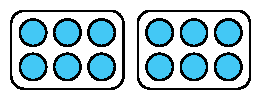
\includegraphics[width=\linewidth]{external/tikz-source/tikz-file-149310.pdf}
\end{sbspanel}%
\begin{sbspanel}{0.5}%
B%
\par
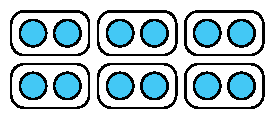
\includegraphics[width=\linewidth]{external/tikz-source/tikz-file-149311.pdf}
\end{sbspanel}%
\end{sidebyside}%
\par\smallskip%
\noindent\textbf{\blocktitlefont Solución}.\hypertarget{act-lapicesColores-3}{}\quad{}A.%
\par
El dibujo B no es correcto pues muestra 6 grupos de 2 lápices de colores. Eso sería como si ella tuviera 6 cajas, en vez de 2 cajas.%
\end{activity}%
\par
\begin{paragraphs}{Síntesis de la actividad.}{act-lapicesColores-5-1}%
MLR1 Más fuerte y cada vez más claro%
%
\begin{itemize}[label=\textbullet]
\item{}``Compartan su respuesta con su compañero. Por turnos, uno habla y el otro escucha. Si es su turno de hablar, compartan sus ideas y lo que han escrito hasta el momento. Si es su turno de escuchar, hagan preguntas y comentarios que ayuden a su compañero a mejorar su trabajo.''%
\item{}2-3 minutos: discusión estructurada en pareja%
\item{}Repetir con 2 compañeros diferentes.%
\item{}``¿Cuál dibujo decidieron que corresponde? ¿Cómo lo saben?''%
\item{}``¿Cómo saben que el otro dibujo no corresponde a esta situación?'' (El dibujo B son 6 grupos de 2 lápices de colores. Eso sería como si tuviera 6 cajas, no 2 cajas.)%
\end{itemize}
\end{paragraphs}%
\end{subsubsectionptx}
%
%
\typeout{************************************************}
\typeout{Subsubsección  Actividad 3~(15 mins)}
\typeout{************************************************}
%
\begin{subsubsectionptx}{Subsubsección}{Actividad 3~(15 mins)}{}{Actividad 3}{}{}{lec-dibujosSituacionesDivision-act3}
\par
\begin{paragraphs}{Tiempo recomendado.}{act-cualDibujoCorresponde-4-1}%
15 minutos.%
\end{paragraphs}%
\begin{paragraphs}{Narrativa.}{act-cualDibujoCorresponde-4-2}%
El propósito de esta actividad es que los estudiantes relacionen situaciones de división y diagramas de grupos iguales (MP2). Cada diagrama dado corresponde a dos situaciones diferentes. Los estudiantes aprenden que el mismo diagrama puede representar tanto un problema de "¿cuántos grupos?" como un problema de "¿cuántos en cada grupo?" porque el diagrama muestra el resultado final, no cómo se formaron los grupos. Cuando los estudiantes interpretan un diagrama como representación de dos tipos de historias diferentes, indican claramente cómo cada parte del diagrama corresponde a la historia, incluyendo lo que corresponde a lo desconocido en la historia (MP6).%
\end{paragraphs}%
\begin{paragraphs}{Lanzamiento.}{act-cualDibujoCorresponde-4-3}%
%
\begin{itemize}[label=\textbullet]
\item{}Grupos de 2%
\item{}``Vamos a examinar algunas situaciones que incluyen herramientas para escribir o dibujar. ¿Qué cosas usamos para escribir o dibujar?''%
\item{}30 segundos: tiempo de reflexión en silencio%
\item{}Compartir y registrar las respuestas.%
\end{itemize}
\end{paragraphs}%
\begin{paragraphs}{Desarrollo de la actividad.}{act-cualDibujoCorresponde-4-4}%
%
\begin{itemize}[label=\textbullet]
\item{}``Van a asociar seis situaciones con dibujos que podrían representarlas. Tómense unos minutos para decidir cuál dibujo corresponde a cada situación.''%
\item{}3-5 minutos: tiempo de trabajo individual%
\item{}``Compartan sus ideas con su compañero.''%
\item{}2-3 minutos: discusión en pareja%
\end{itemize}
\end{paragraphs}%
\begin{activity}{Actividad}{¿Cuál dibujo corresponde?}{act-cualDibujoCorresponde}%
Asocia cada situación con un dibujo. Prepárate para explicar tu razonamiento.%
\begin{sidebyside}{2}{0}{0}{0.05}%
\begin{sbspanel}{0.55}[center]%
%
\begin{enumerate}
\item{}Mai tiene 8 marcadores y varias cajas. Ella pone 4 marcadores en cada caja. ¿Cuántas cajas con marcadores hay?%
\item{}Kiran tiene 20 bolígrafos y varias mesas. Él pone 2 bolígrafos en cada mesa. ¿En cuántas mesas puede poner bolígrafos?%
\item{}Lin tiene 8 lápices de colores y 2 bolsas. En cada bolsa pone el mismo número de lápices de colores. ¿Cuántos lápices de colores habrá en cada bolsa?%
\item{}Priya tiene 15 crayones y varios pupitres. Ella pone 5 crayones en cada pupitre. ¿En cuántos pupitres pondrá crayones?%
\item{}Noah tiene 20 lápices y 10 cajas. Él pone el mismo número de lápices en cada caja. ¿Cuántos lápices habrá en cada caja?%
\item{}Jada tiene 15 marcadores y 3 mesas. Ella pone el mismo número de marcadores en cada mesa. ¿Cuántos marcadores habrá en cada mesa?%
\end{enumerate}
\end{sbspanel}%
\begin{sbspanel}{0.4}[center]%
A.%
\par
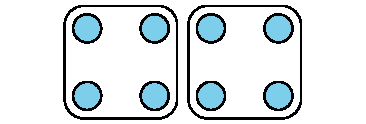
\includegraphics[width=\linewidth]{external/svg-source/tikz-file-149313.pdf}
B.%
\par
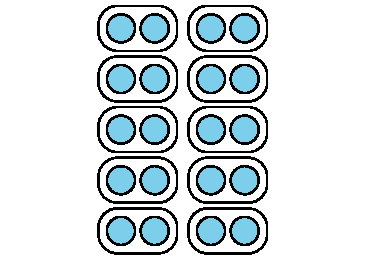
\includegraphics[width=\linewidth]{external/svg-source/tikz-file-149314.pdf}
C.%
\par
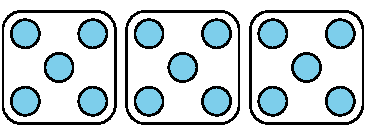
\includegraphics[width=\linewidth]{external/svg-source/tikz-file-149315.pdf}
\end{sbspanel}%
\end{sidebyside}%
\par\smallskip%
\noindent\textbf{\blocktitlefont Solución}.\hypertarget{act-cualDibujoCorresponde-3}{}\quad{}Respuesta del enunciado%
%
\begin{enumerate}
\item{}A%
\item{}B%
\item{}A%
\item{}C%
\item{}B%
\item{}C%
\end{enumerate}
\end{activity}%
\par
\begin{paragraphs}{Para los estudiantes con dificultades.}{act-cualDibujoCorresponde-5-1}%
Si los estudiantes dicen que el dibujo no puede representar ambas situaciones, considere preguntar:%
%
\begin{itemize}[label=\textbullet]
\item{}``¿Cómo podríamos hacer un dibujo para cada situación?''%
\item{}``¿Qué podríamos dibujar primero para representar la primera situación en la que hay 8 objetos? ¿Y para la segunda situación en la que hay 8 objetos?''%
\end{itemize}
\end{paragraphs}%
\begin{paragraphs}{Síntesis de la actividad.}{act-cualDibujoCorresponde-5-2}%
%
\begin{itemize}[label=\textbullet]
\item{}Invite a los estudiantes a compartir qué dibujo corresponde a cada situación.%
\item{}Enfóquese en un dibujo y las dos situaciones que puede representar, como:%
\begin{image}{0}{1}{0}{}%
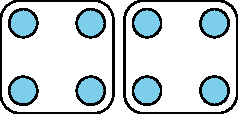
\includegraphics[width=\linewidth]{external/svg-source/tikz-file-149312.pdf}
\end{image}%
%
\begin{itemize}[label=$\circ$]
\item{}Mai tiene 8 marcadores. Ella pone 4 marcadores en cada caja. ¿Cuántas cajas de marcadores hay?%
\item{}Lin tiene 8 lápices de colores y 2 bolsas. Cada bolsa tiene la misma cantidad de lápices de colores. ¿Cuántos lápices de colores habrá en cada bolsa?%
\end{itemize}
\item{}``¿Cómo puede el mismo dibujo representar ambas situaciones?'' (No vimos cómo se formaron los grupos, pero al final se formaron la misma cantidad de grupos y grupos del mismo tamaño en ambas situaciones. El dibujo puede representar la situación de poner 8 marcadores en cajas con 4 marcadores en cada caja y encontrar que se necesitan 2 cajas. También puede representar la situación de poner 8 lápices en 2 bolsas con la misma cantidad de lápices en cada bolsa y encontrar que se pueden poner 4 lápices en cada bolsa.)%
\end{itemize}
\end{paragraphs}%
\begin{paragraphs}{Desarrollo de lenguaje matemático.}{act-cualDibujoCorresponde-5-3}%
Apoyos para la discusión (MLR8). Los estudiantes deben turnarse para encontrar una correspondencia y explicar su razonamiento a su compañero.%
\par
Muestre el siguiente esquema de oración para que todos lo vean: "Observé \textunderscore{}\textunderscore{}\textunderscore{}, entonces asocié . . ."%
\par
Motívelos a desafiarse mutuamente cuando no estén de acuerdo.%
\end{paragraphs}%
\begin{paragraphs}{Acceso a estudiantes con discapacidades.}{act-cualDibujoCorresponde-5-4}%
Proporcione acceso al generar interés. Aproveche la elección en torno al desafío percibido. Invite a los estudiantes a seleccionar al menos 3 de los 6 problemas para completar.%
\par
Apoya la accesibilidad para: Organización, Atención, Habilidades socioemocionales.%
\end{paragraphs}%
\end{subsubsectionptx}
%
%
\typeout{************************************************}
\typeout{Subsubsección  Síntesis de la lección~(5 mins)}
\typeout{************************************************}
%
\begin{subsubsectionptx}{Subsubsección}{Síntesis de la lección~(5 mins)}{}{Síntesis de la lección~(5 mins)}{}{}{lec-dibujosSituacionesDivision-sintesis}
Tiempo recomendado: 10 mins.%
\par
``Hoy asociamos dibujos con situaciones de división. Hay dos tipos de situaciones de división y hoy vimos que el mismo dibujo puede representar ambos tipos de situaciones.''%
\par
Considera este grupo:%
\begin{sidebyside}{3}{0.00833333333333333}{0.00833333333333333}{0.0166666666666667}%
\begin{sbspanel}{0.25}%
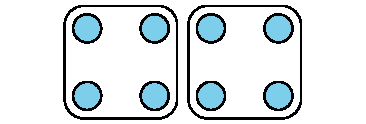
\includegraphics[width=\linewidth]{external/svg-source/tikz-file-149313.pdf}
\end{sbspanel}%
\begin{sbspanel}{0.35}%
Mai tiene 8 marcadores y varias cajas. Ella pone 4 marcadores en cada caja. ¿Cuántas cajas con marcadores hay?%
\end{sbspanel}%
\begin{sbspanel}{0.35}%
\par
Lin tiene 8 lápices de colores y 2 bolsas. En cada bolsa pone el mismo número de lápices de colores. ¿Cuántos lápices de colores habrá en cada bolsa?%
\end{sbspanel}%
\end{sidebyside}%
\par
``¿En qué se parecen y en qué se diferencian estas situaciones de división?'' (Ambas situaciones tienen los números 8, 2 y 4 en ellas. Ambas involucran poner objetos en grupos iguales. Los objetos son diferentes, una se trata de marcadores y la otra de lápices de colores. Una situación nos dice cuántos elementos van en cada contenedor y la otra nos dice cuántos contenedores hay)%
\par
``En la primera situación, debemos averiguar cuántos grupos hay. Sabemos que hay 4 marcadores en cada caja, pero no sabemos cuántas cajas hay. En la segunda situación, debemos averiguar cuántos hay en cada grupo. Sabemos que hay 2 bolsas, pero no sabemos cuántos lápices de colores hay en cada bolsa.''%
\par
``Ahora que estamos dividiendo, necesitamos un símbolo nuevo para escribir expresiones de división. Si queremos representar "8 dividido en grupos de 4", escribimos: \(8\div 4\).''%
\par
``¿Qué expresión podríamos escribir para representar "8 dividido en 2 grupos"?'' (\(8\div2\))%
\end{subsubsectionptx}
%
%
\typeout{************************************************}
\typeout{Preguntas de comprensión  Actividad de cierre~(5 mins)}
\typeout{************************************************}
%
\begin{reading-questions-subsubsection}{Preguntas de comprensión}{Actividad de cierre~(5 mins)}{}{Actividad de cierre}{}{}{lec-dibujosSituacionesDivision-cool}
\href{external/cools-pdf/cool-regalitosInvitados-standalone.pdf}{Descargar pdf para imprimir o proyectar}\footnote{\nolinkurl{external/cools-pdf/cool-regalitosInvitados-standalone.pdf}\label{lec-dibujosSituacionesDivision-cool-5}}\begin{project}{Actividad de cierre}{Regalitos para invitados.}{cool-regalitosInvitados}%
Clare tiene 48 marcadores. Ella pone 8 marcadores en cada bolsa de regalitos para su fiesta de cumpleaños. ¿Cuántas bolsas usará?%
\par
¿Cuál dibujo corresponde a la situación? Explica tu razonamiento.%
\begin{sidebyside}{2}{0}{0}{0}%
\begin{sbspanel}{0.5}%
A.%
\par
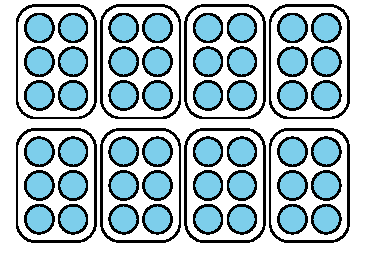
\includegraphics[width=\linewidth]{external/svg-source/tikz-file-246306.pdf}
\end{sbspanel}%
\begin{sbspanel}{0.5}%
B.%
\par
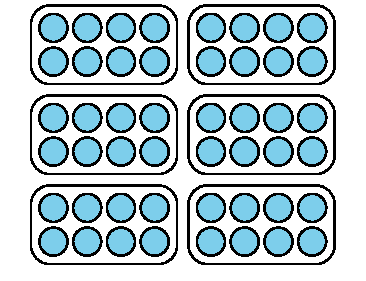
\includegraphics[width=\linewidth]{external/svg-source/tikz-file-246307.pdf}
\end{sbspanel}%
\end{sidebyside}%
\par\smallskip%
\noindent\textbf{\blocktitlefont Solución}.\hypertarget{cool-regalitosInvitados-3}{}\quad{}Respuesta de ejemplo: El dibujo B corresponde a la situación porque muestra 8 marcadores en cada bolsa. Después de que los 48 marcadores se dividan en grupos de 8, habrá 6 bolsas.%
\end{project}%
\par
\begin{paragraphs}{Posibles errores.}{cool-regalitosInvitados-4-1}%
Los estudiantes eligen el dibujo A, que muestra 8 bolsas en lugar de 8 marcadores en cada bolsa.%
\end{paragraphs}%
\begin{paragraphs}{Acciones para apoyar el aprendizaje.}{cool-regalitosInvitados-4-2}%
Durante el lanzamiento de la actividad del día siguiente, haga que los estudiantes discutan por qué el dibujo B corresponde a la situación.%
\end{paragraphs}%
\end{reading-questions-subsubsection}
\end{subsectionptx}
%
%
\typeout{************************************************}
\typeout{Subsección  Lección 4 -~Interpretemos expresiones de división}
\typeout{************************************************}
%
\begin{subsectionptx}{Subsección}{Lección 4 -~Interpretemos expresiones de división}{}{Lección 4}{}{}{lec-interpretarExpresionesDivision}
\begin{objectives}{Objetivos de aprendizaje}{lec-interpretarExpresionesDivision-4}
%
\begin{itemize}[label=\textbullet]
\item{}Interpretar expresiones de división.%
\item{}Comprender que se puede utilizar la misma expresión de división para representar ambos tipos de situaciones de división.%
\end{itemize}
\end{objectives}
\begin{introduction}{}%
\begin{paragraphs}{Estándares CCSS asociados.}{lec-interpretarExpresionesDivision-5-1}%
3.NBT.A.2, 3.OA.A.2%
\end{paragraphs}%
\begin{paragraphs}{Momentos de la lección.}{lec-interpretarExpresionesDivision-5-2}%
\noindent
\begin{longtable}[l]{ll}
\addtocounter{table}{-1}
\endfirsthead
\endhead
\multicolumn{2}{r}{(Continúa en la página siguiente)}\\
\endfoot
\endlastfoot
\hyperref[lec-interpretarExpresionesDivision-warm]{Subsubsección }& Calentamiento~(10 mins)\\
\hyperref[lec-interpretarExpresionesDivision-act1]{Subsubsección }& Actividad 1~(10 mins)\\
\hyperref[lec-interpretarExpresionesDivision-act2]{Subsubsección }& Actividad 2~(10 mins)\\
\hyperref[lec-interpretarExpresionesDivision-act3]{Subsubsección }& Actividad 3~(15 mins)\\
\hyperref[lec-interpretarExpresionesDivision-sintesis]{Subsubsección }& Síntesis de la lección~(10 mins)\\
\hyperref[lec-interpretarExpresionesDivision-cool]{Preguntas de comprensión }& Actividad de cierre~(5 mins)\\
\end{longtable}
\end{paragraphs}%
\begin{paragraphs}{Propósito de la lección.}{lec-interpretarExpresionesDivision-5-3}%
El propósito de esta lección es que los estudiantes interpreten expresiones de división y comprendan que pueden utilizar la misma expresión de división para representar ambos tipos de situaciones de división.%
\end{paragraphs}%
\begin{paragraphs}{Narrativa de la lección.}{lec-interpretarExpresionesDivision-5-4}%
Los estudiantes primero emparejan una expresión de división con una situación que podría representar. Luego, aprenden que la misma expresión de división puede corresponder tanto a problemas de "¿cuántos grupos?" como a problemas de "¿cuántos en cada grupo?", dependiendo de cómo se interprete el divisor (el número por el cual estamos dividiendo). Luego, los estudiantes tienen la oportunidad de emparejar dibujos y expresiones con situaciones antes de escribir sus propias expresiones de división en una lección posterior.%
\end{paragraphs}%
\begin{paragraphs}{Preguntas de reflexión.}{lec-interpretarExpresionesDivision-5-5}%
¿Qué aspectos de la lección de hoy permitieron a cada uno de sus estudiantes verse a sí mismo como un pensador matemático productivo?%
\end{paragraphs}%
\end{introduction}%
%
%
\typeout{************************************************}
\typeout{Subsubsección  Calentamiento~(10 mins)}
\typeout{************************************************}
%
\begin{subsubsectionptx}{Subsubsección}{Calentamiento~(10 mins)}{}{Calentamiento}{}{}{lec-interpretarExpresionesDivision-warm}
\par
\begin{paragraphs}{Tiempo recomendado.}{act-numTalk-masOMenos-4-1}%
10 minutos%
\end{paragraphs}%
\begin{paragraphs}{Narrativa.}{act-numTalk-masOMenos-4-2}%
El propósito de esta conversación numérica es generar un espacio para recordar las estrategias y comprensiones que los estudiantes usan cuando restan hasta 1,000 (es decir, sin que los números ni el resultado se pasen de 1,000), especialmente al sumar para encontrar diferencias. Estas comprensiones ayudan a los estudiantes a desarrollar fluidez para restar hasta 1,000.%
\end{paragraphs}%
\begin{paragraphs}{Lanzamiento.}{act-numTalk-masOMenos-4-3}%
%
\begin{itemize}[label=\textbullet]
\item{}Muestre una expresión.%
\item{}``Hagan una señal cuando tengan una respuesta y puedan explicar cómo la obtuvieron.''%
\item{}1 minuto: tiempo de reflexión en silencio%
\end{itemize}
\end{paragraphs}%
\begin{paragraphs}{Desarrollo de la actividad.}{act-numTalk-masOMenos-4-4}%
%
\begin{itemize}[label=\textbullet]
\item{}Registre las respuestas y las estrategias.%
\item{}Mantenga las expresiones y el trabajo visible.%
\item{}Repita con cada expresión.%
\end{itemize}
\end{paragraphs}%
\begin{exploration}{Calentamiento}{Conversación numérica: ¿Más o menos?}{act-numTalk-masOMenos}%
Encuentra mentalmente el valor de cada expresión.%
%
\begin{enumerate}[label={\Alph*.}]
\item{}\(\displaystyle 500 - 475\)%
\item{}\(\displaystyle 504 - 475\)%
\item{}\(\displaystyle 512 - 475\)%
\item{}\(\displaystyle 512 - 449\)%
\end{enumerate}
\par\smallskip%
\noindent\textbf{\blocktitlefont Solución}.\hypertarget{act-numTalk-masOMenos-3}{}\quad{}Ejemplos de respuestas%
\par
%
\begin{enumerate}[label={\Alph*.}]
\item{}25. Le sumé 25 a 475 para llegar a 500.%
\item{}29. Pensé en el primer problema y le sumé 4 a 25 para llegar a 504.%
\item{}37. Comencé en 475 y le sumé 25 para llegar a 500. Luego, le sumé 10 para llegar a 510 y le sumé 2 más para llegar a 512. \(25 + 10 + 2 = 37\).%
\item{}63. Sé que a 449 le faltan 51 para llegar a 500 y después le sumé 12 más a 51.%
\end{enumerate}
%
\end{exploration}%
\par
\begin{paragraphs}{Síntesis de la actividad.}{act-numTalk-masOMenos-5-1}%
%
\begin{itemize}[label=\textbullet]
\item{}``¿Por qué el valor de \(512 - 475\) es mayor que el valor de \(504 - 475\)?'' (Dado que el 475 no cambia, pero 512 es mayor que 504, la diferencia entre los números es mayor.)%
\item{}Considere preguntar:%
\begin{itemize}[label=$\circ$]
\item{}``¿Alguien puede expresar el razonamiento de \fillintext{10} de otra forma?''%
\item{}``¿Alguien usó la misma estrategia, pero la explicaría de otra forma?''%
\item{}``¿Alguien pensó en el problema de otra forma?''%
\item{}``¿Alguien quiere agregar algo a la estrategia de \fillintext{10}?''%
\end{itemize}
%
\end{itemize}
\end{paragraphs}%
\end{subsubsectionptx}
%
%
\typeout{************************************************}
\typeout{Subsubsección  Actividad 1~(10 mins)}
\typeout{************************************************}
%
\begin{subsubsectionptx}{Subsubsección}{Actividad 1~(10 mins)}{}{Actividad 1}{}{}{lec-interpretarExpresionesDivision-act1}
\par
\begin{paragraphs}{Tiempo recomendado.}{act-trompos-4-1}%
10 minutos%
\end{paragraphs}%
\begin{paragraphs}{Narrativa.}{act-trompos-4-2}%
El propósito de esta actividad es que los estudiantes emparejen expresiones de división con situaciones de división. Los estudiantes deben justificar sus elecciones explicando claramente cómo se conectan los números en la expresión con lo que está sucediendo en la situación (MP2).%
\end{paragraphs}%
\begin{paragraphs}{Lanzamiento.}{act-trompos-4-3}%
%
\begin{itemize}[label=\textbullet]
\item{}Grupos de 2%
\item{}Muestre la imagen.%
\item{}``Estos juguetes se llaman trompos. En muchas culturas se juega con ellos. ¿Qué otros juguetes conocen?''%
\item{}30 segundos: tiempo para pensar en silencio%
\item{}Compartan las respuestas.%
\item{}``Ahora vamos a trabajar con algunas situaciones que incluyen trompos. Más adelante, vamos a ver situaciones sobre otros juguetes.''%
\end{itemize}
\end{paragraphs}%
\begin{paragraphs}{Desarrollo de la actividad.}{act-trompos-4-4}%
%
\begin{itemize}[label=\textbullet]
\item{}``Con su compañero, emparejen cada situación con una expresión de división.''%
\item{}3-5 minutos: tiempo de trabajo en parejas%
\item{}Identifique a los estudiantes que puedan justificar sus emparejamientos explicando cómo los números en la expresión representan la situación.%
\end{itemize}
\end{paragraphs}%
\begin{activity}{Actividad}{Trompos.}{act-trompos}%
Los trompos son populares en todo el mundo. Estos son trompos de diferentes culturas.%
\begin{sidebyside}{5}{0}{0}{0}%
\begin{sbspanel}{0.2}%
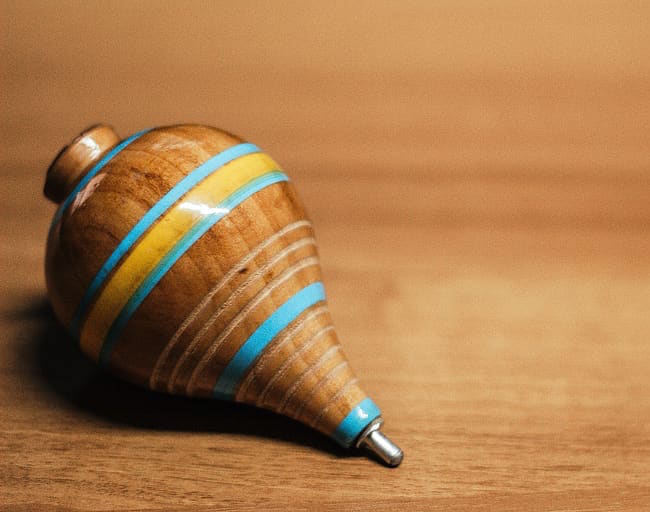
\includegraphics[width=\linewidth]{external/jpg-source/V1 3.4.A.4 Mexican Trompo.jpg}
\end{sbspanel}%
\begin{sbspanel}{0.2}%
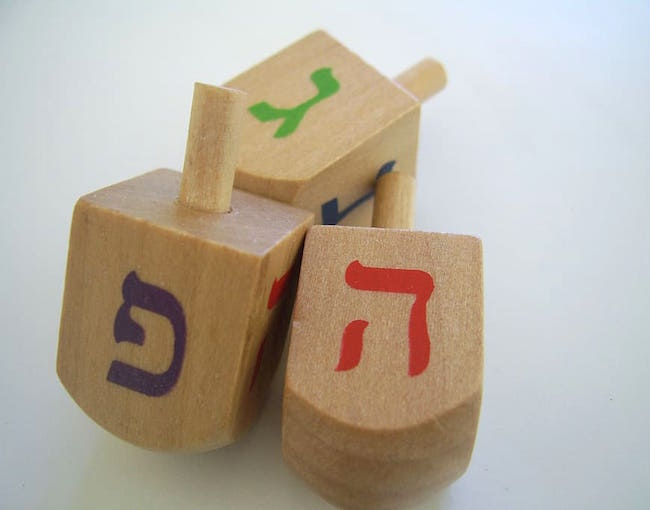
\includegraphics[width=\linewidth]{external/jpg-source/V1 3.4.A.4 Dreidels.jpg}
\end{sbspanel}%
\begin{sbspanel}{0.2}%
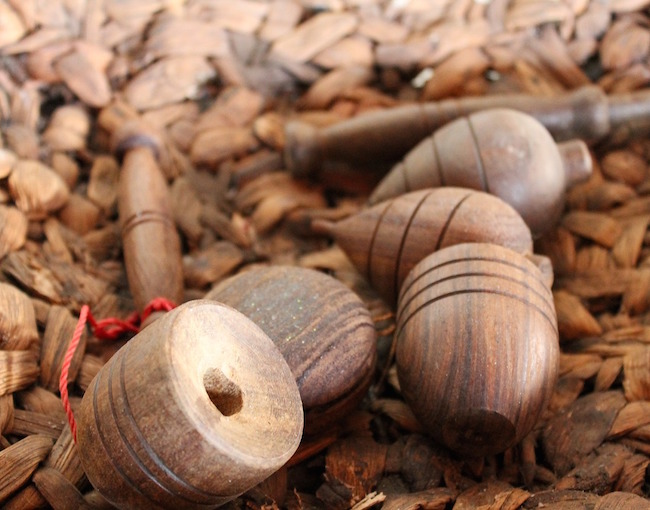
\includegraphics[width=\linewidth]{external/jpg-source/V1 3.4.A.4 Indonesian Gasing.jpg}
\end{sbspanel}%
\begin{sbspanel}{0.2}%
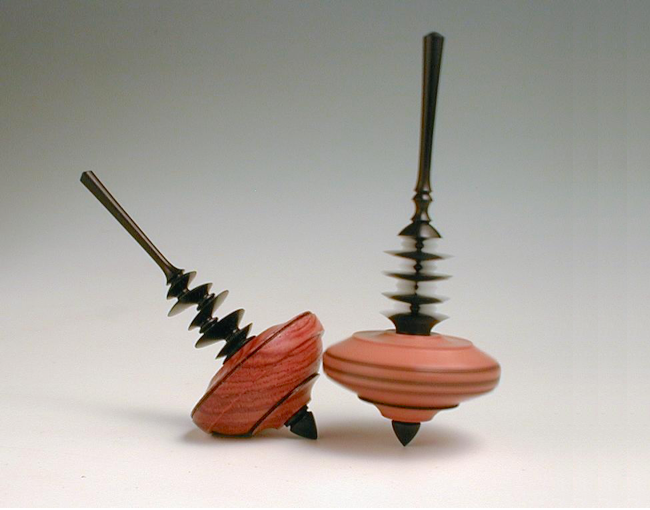
\includegraphics[width=\linewidth]{external/png-source/V1 3.4.A.4 German Kreisel Copy.png}
\end{sbspanel}%
\begin{sbspanel}{0.2}%
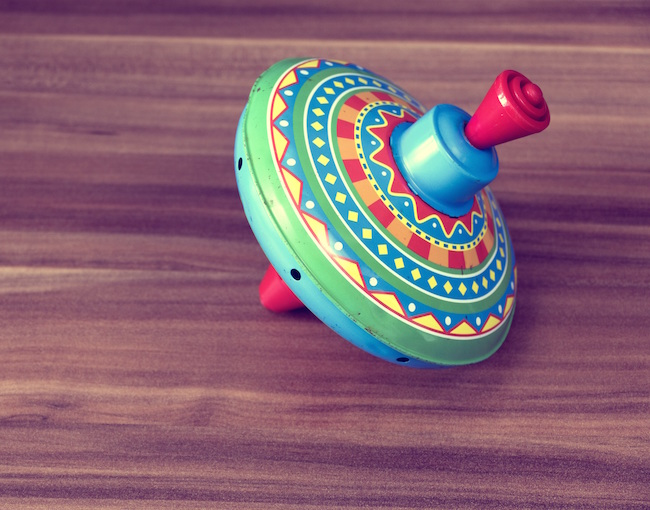
\includegraphics[width=\linewidth]{external/jpg-source/V1 3.4.A.4 Colorful Top.jpg}
\end{sbspanel}%
\end{sidebyside}%
\par
Empareja cada situación sobre trompos con una expresión que pueda representarla.%
\begin{sidebyside}{2}{0.05}{0}{0.15}%
\begin{sbspanel}{0.6}%
1. Clare tiene una colección de 24 trompos de cuatro colores: negro, blanco, rojo y verde. Tiene el mismo número de trompos de cada color. ¿Cuántos trompos tiene de cada color?%
\end{sbspanel}%
\begin{sbspanel}{0.2}%
\par
A. \(24 \div 2\)%
\end{sbspanel}%
\end{sidebyside}%
\begin{sidebyside}{2}{0.05}{0}{0.15}%
\begin{sbspanel}{0.6}%
2. Priya y su amigo están decorando con pintura 24 trompos de madera. Si cada uno pinta el mismo número de trompos, ¿cuántos trompos pinta cada uno?%
\end{sbspanel}%
\begin{sbspanel}{0.2}%
\par
B. \(12 \div 2\)%
\end{sbspanel}%
\end{sidebyside}%
\begin{sidebyside}{2}{0.05}{0}{0.15}%
\begin{sbspanel}{0.6}%
3. En una tienda tienen 24 trompos de distintas partes del mundo exhibidos en 6 cajas. Cada caja contiene el mismo número de trompos. ¿Cuántos trompos hay en cada caja?%
\end{sbspanel}%
\begin{sbspanel}{0.2}%
\par
C. \(24 \div 4\)%
\end{sbspanel}%
\end{sidebyside}%
\begin{sidebyside}{2}{0.05}{0}{0.15}%
\begin{sbspanel}{0.6}%
4. Diego tiene 12 trompos que quiere regalar. Si a cada amigo le da 2 trompos, ¿cuántos amigos recibirán trompos?%
\end{sbspanel}%
\begin{sbspanel}{0.2}%
\par
D. \(12 \div 6\)%
\end{sbspanel}%
\end{sidebyside}%
\begin{sidebyside}{2}{0.05}{0}{0.15}%
\begin{sbspanel}{0.6}%
5. Seis amigos están jugando con 12 \emph{dreidels} (trompos judíos). Si cada uno juega con el mismo número de \emph{dreidels} que los demás, ¿cuántos \emph{dreidels} tiene cada uno?%
\end{sbspanel}%
\begin{sbspanel}{0.2}%
\par
E. \(24 \div 6\)%
\end{sbspanel}%
\end{sidebyside}%
\par\smallskip%
\noindent\textbf{\blocktitlefont Solución}.\hypertarget{act-trompos-3}{}\quad{}1:C, 2:A, 3:E, 4:B, 5:D%
\end{activity}%
\footnotetext[26]{\nolinkurl{pixabay.com/photos/wooden-spinning-top-top-mexican-3868460/}\label{act-trompos-2-2-1-2-1-2}}%
\footnotetext[27]{\nolinkurl{pixabay.com/photos/dreidels-hanukkah-spinning-tops-20347/}\label{act-trompos-2-2-2-2-1-2}}%
\footnotetext[28]{\nolinkurl{pixabay.com/photos/whirligig-traditional-folklore-wood-2316859/}\label{act-trompos-2-2-3-2-1-2}}%
\footnotetext[29]{\nolinkurl{commons.wikimedia.org/wiki/File:Spinning_Top.jpeg}\label{act-trompos-2-2-4-2-1-2}}%
\footnotetext[30]{\nolinkurl{www.pexels.com/photo/blue-and-green-spin-toy-170288/}\label{act-trompos-2-2-5-2-1-2}}%
\par
\begin{paragraphs}{Síntesis de la actividad.}{act-trompos-5-1}%
%
\begin{itemize}[label=\textbullet]
\item{}Seleccione a los estudiantes identificados para compartir.%
\item{}Considere preguntar: ``¿Cómo representan los números de la expresión lo que hay en la situación?''%
\end{itemize}
\end{paragraphs}%
\end{subsubsectionptx}
%
%
\typeout{************************************************}
\typeout{Subsubsección  Actividad 2~(10 mins)}
\typeout{************************************************}
%
\begin{subsubsectionptx}{Subsubsección}{Actividad 2~(10 mins)}{}{Actividad 2}{}{}{lec-interpretarExpresionesDivision-act2}
\par
\begin{paragraphs}{Tiempo recomendado.}{act-autosCajas-4-1}%
10 minutos%
\end{paragraphs}%
\begin{paragraphs}{Narrativa.}{act-autosCajas-4-2}%
El propósito de esta actividad es que los estudiantes comprendan que pueden utulizar la misma expresión de división para representar ambos tipos de situaciones de división. A los estudiantes se les dan dos situaciones y se les pide que emparejen una expresión de división con una de las situaciones, pero la expresión coincide con las dos situaciones dadas. Está bien si, durante el desarrollo de la actividad, los estudiantes no reconocen que la expresión coincide con ambas situaciones, porque se discutirá en la síntesis de la actividad. Los estudiantes aprenden que el número por el cual estamos dividiendo se llama divisor y comprenden que el divisor puede representar el tamaño de los grupos o el número de grupos. Cuando los estudiantes explican que un divisor se puede interpretar de manera diferente según la situación que representa, razonan abstracta y cuantitativamente (MP2).%
\end{paragraphs}%
\begin{paragraphs}{Lanzamiento.}{act-autosCajas-4-3}%
%
\begin{itemize}[label=\textbullet]
\item{}Grupos de 2%
\item{}``Examinemos un poco más de cerca las expresiones de división. Tómense un minuto para leer estas dos situaciones de manera individual.''%
\item{}1 minuto: tiempo para pensar en silencio%
\end{itemize}
\end{paragraphs}%
\begin{paragraphs}{Desarrollo de la actividad.}{act-autosCajas-4-4}%
%
\begin{itemize}[label=\textbullet]
\item{}``Trabajen con su compañero para decidir qué situación representa la expresión \(21\div3\).''%
\item{}2-3 minutos: tiempo de trabajo en pareja%
\end{itemize}
\end{paragraphs}%
\begin{activity}{Actividad}{Autos en cajas.}{act-autosCajas}%
Considera estas dos situaciones.%
\begin{sidebyside}{2}{0.05}{0.05}{0.1}%
\begin{sbspanel}{0.4}%
A. Han tiene 21 autos de juguete y 3 cajas. Él pone el mismo número de autos en cada caja. ¿Cuántos autos habrá en cada caja?%
\end{sbspanel}%
\begin{sbspanel}{0.4}%
\par
B. Han tiene 21 autos de juguete y varias cajas. Él quiere poner 3 autos en cada caja. ¿Cuántas cajas necesitará?%
\end{sbspanel}%
\end{sidebyside}%
\par
¿Cuál situación está representada por la expresión \(21\div 3\)? Explica tu razonamiento.%
\par\smallskip%
\noindent\textbf{\blocktitlefont Solución}.\hypertarget{act-autosCajas-3}{}\quad{}Ejemplos de respuestas%
\par
Ambas situaciones están representadas por la expresión \(21\div 3\). El 3 en la situación A es en número de cajas y el 3 en la situación B es el número de autos que van en cada caja.%
\end{activity}%
\par
\begin{paragraphs}{Síntesis de la actividad.}{act-autosCajas-5-1}%
%
\begin{itemize}[label=\textbullet]
\item{}Invite a los estudiantes a compartir sus respuestas y razonamientos.%
\item{}``¿Cómo puede la misma expresión representar dos situaciones diferentes?'' (Ambas situaciones involucran los mismos números, 21 y 3. Ambas situaciones involucran poner 21 objetos en grupos iguales. En un caso, el 3 es el número de objetos en el grupo, pero en el otro, 3 es el número de grupos. Ambas situaciones hablan de 21 dividido entre 3, solo que de diferentes maneras.)%
\item{}``Observamos que el número entre el que estamos dividiendo, 3, puede tener dos significados diferentes. Puede significar 3 grupos o 3 objetos en cada grupo.''%
\item{}``Cuando dividimos, el número entre el que dividimos se llama el \terminology{divisor}. En la expresión \(27\div 3\), el divisor es 3.''%
\end{itemize}
\end{paragraphs}%
\begin{paragraphs}{Desarrollo de lenguaje matemático.}{act-autosCajas-5-2}%
MLR2 Recopilar y Mostrar. Recorra el salón y recopile el lenguaje que los estudiantes usan mientras consideran las dos situaciones. Escuche y aclare cualquier pregunta sobre el contexto. En una presentación visible, registre palabras y frases como: poner en grupos, dividir, número de grupos, etc. Durante la síntesis, agregue "divisor" a la presentación y resalte las conexiones con cualquier lenguaje relacionado.%
\par
Avances: Conversación, Lectura%
\end{paragraphs}%
\end{subsubsectionptx}
%
%
\typeout{************************************************}
\typeout{Subsubsección  Actividad 3~(15 mins)}
\typeout{************************************************}
%
\begin{subsubsectionptx}{Subsubsección}{Actividad 3~(15 mins)}{}{Actividad 3}{}{}{lec-interpretarExpresionesDivision-act3}
\par
\begin{paragraphs}{Tiempo recomendado.}{act-pilasBloques-4-1}%
15 minutos.%
\end{paragraphs}%
\begin{paragraphs}{Narrativa.}{act-pilasBloques-4-2}%
El propósito de esta actividad es que los estudiantes apliquen lo que han aprendido sobre las representaciones de la división para relacionar dibujos y expresiones con situaciones de división (MP2). Al hacerlo, solidifican su comprensión de que la misma expresión de división puede representar ambos tipos de situaciones de división. Los dibujos dados permiten a los estudiantes ver la cantidad de grupos y cuántos objetos hay en cada grupo. El trabajo aquí ayuda a los estudiantes a hacer conexiones entre las tres representaciones antes de que escriban sus propias expresiones de división y resuelvan problemas de división en una lección posterior. Cuando los estudiantes describen cómo una expresión puede representar diferentes historias, prestan atención a la precisión en el lenguaje que utilizan y a la correspondencia que establecen entre la expresión y las historias (MP6).%
\end{paragraphs}%
\begin{paragraphs}{Lanzamiento.}{act-pilasBloques-4-3}%
%
\begin{itemize}[label=\textbullet]
\item{}Grupos de 2%
\item{}``Ahora que hemos representado situaciones de división con dibujos y con expresiones, vamos a asociar algunas situaciones con ambas representaciones.''%
\item{}``Lean estas situaciones de manera individual.''%
\item{}1-2 minutos: tiempo de reflexión en silencio%
\item{}``Discutan con su compañero en qué se parecen y en qué se diferencian estas situaciones.''%
\item{}2-3 minutos: discusión en pareja%
\item{}Compartan las respuestas.%
\end{itemize}
\end{paragraphs}%
\begin{paragraphs}{Desarrollo de la actividad.}{act-pilasBloques-4-4}%
%
\begin{itemize}[label=\textbullet]
\item{}``Ahora, con su compañero, asocien cada situación con un dibujo y con una expresión que representan la situación''%
\item{}3-5 minutos: tiempo de trabajo en pareja%
\end{itemize}
\end{paragraphs}%
\begin{activity}{Actividad}{Pilas de bloques.}{act-pilasBloques}%
Asocia cada situación con un dibujo y con una expresión que representan la situación. Prepárate para explicar tu razonamiento.%
%
\begin{enumerate}
\item{}Kiran usa 6 bloques para hacer pilas. Cada pila tiene 2 bloques. ¿Cuántas pilas hay?%
\item{}Han usa 6 bloques para hacer dos pilas iguales. ¿Cuántos bloques hay en cada pila?%
\item{}Jada usa 6 bloques para construir pilas que tienen 3 bloques cada una. ¿Cuántas pilas hay?%
\item{}Mai usa 6 bloques para hacer 3 pilas iguales. ¿Cuántos bloques hay en cada pila?%
\end{enumerate}
Dibujos%
\begin{sidebyside}{2}{0.05}{0.05}{0.1}%
\begin{sbspanel}{0.4}%
A%
\par
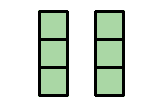
\includegraphics[width=\linewidth]{external/svg-source/tikz-file-149316.pdf}
\end{sbspanel}%
\begin{sbspanel}{0.4}%
B%
\par
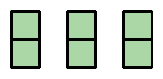
\includegraphics[width=\linewidth]{external/svg-source/tikz-file-149317.pdf}
\end{sbspanel}%
\end{sidebyside}%
\par
Expresiones%
\begin{sidebyside}{2}{0.05}{0.05}{0.1}%
\begin{sbspanel}{0.4}%
C%
\begin{equation*}
6\div 2
\end{equation*}
%
\end{sbspanel}%
\begin{sbspanel}{0.4}%
\par
D%
\begin{equation*}
6\div 3
\end{equation*}
%
\end{sbspanel}%
\end{sidebyside}%
\par\smallskip%
\noindent\textbf{\blocktitlefont Solución}.\hypertarget{act-pilasBloques-3}{}\quad{}%
\begin{enumerate}
\item{}B y C%
\item{}A y C%
\item{}A y D%
\item{}B y D%
\end{enumerate}
%
\end{activity}%
\par
\begin{paragraphs}{Síntesis de la actividad.}{act-pilasBloques-5-1}%
%
\begin{itemize}[label=\textbullet]
\item{}``Consideremos las primeras dos situaciones sobre Kiran y Han. ¿Por qué podemos usar la misma expresión para representar estas situaciones, pero tenemos que usar dibujos diferentes?'' (Ambas situaciones se representan con 6 dividido entre 2, pero en la primera situación el 2, o el divisor, es la cantidad de bloques en cada pila. En la segunda situación, el 2 es el número de pilas.)%
\item{}``Ahora examinemos las situaciones de Han y Jada. ¿Por qué podemos usar el mismo dibujo para representar estas situaciones, pero no la misma expresión?'' (Ambas situaciones describen 2 grupos de 3, por lo que coinciden con el mismo dibujo. La primera situación es de 6 bloques divididos entre 2 pilas y la segunda situación es de 6 bloques divididos en grupos de 3.)%
\end{itemize}
\end{paragraphs}%
\end{subsubsectionptx}
%
%
\typeout{************************************************}
\typeout{Subsubsección  Síntesis de la lección~(10 mins)}
\typeout{************************************************}
%
\begin{subsubsectionptx}{Subsubsección}{Síntesis de la lección~(10 mins)}{}{Síntesis de la lección~(10 mins)}{}{}{lec-interpretarExpresionesDivision-sintesis}
Tiempo recomendado: 10 mins.%
\par
Muestre algunas expresiones, como estas:%
\begin{equation*}
6\div 2
\end{equation*}
%
\begin{equation*}
6\div 3
\end{equation*}
%
\par
``¿Hay alguna manera de distinguir las expresiones que representan un problema de "¿cuántos grupos?" de las expresiones que representan un problema de "¿cuántos hay en cada grupo?"?'' (No, no solo mirando la expresión. Tendríamos que volver a mirar la situación o el dibujo.)%
\par
``Las expresiones de división se pueden interpretar de dos formas y no podemos realmente saber qué tipo de situación de división representa, a menos de que tengamos una situación o un dibujo que vaya con la expresión.''%
\end{subsubsectionptx}
%
%
\typeout{************************************************}
\typeout{Preguntas de comprensión  Actividad de cierre~(5 mins)}
\typeout{************************************************}
%
\begin{reading-questions-subsubsection}{Preguntas de comprensión}{Actividad de cierre~(5 mins)}{}{Actividad de cierre}{}{}{lec-interpretarExpresionesDivision-cool}
\href{external/cools-pdf/cool-losTromposDe-standalone.pdf}{Descargar pdf para imprimir o proyectar}\footnote{\nolinkurl{external/cools-pdf/cool-losTromposDe-standalone.pdf}\label{lec-interpretarExpresionesDivision-cool-5}}\begin{project}{Actividad de cierre}{Los trompos de Han.}{cool-losTromposDe}%
Han tiene 14 trompos. Él reparte los trompos equitativamente en 2 cajas (es decir, deja la misma cantidad de trompos en cada caja). ¿Cuántos trompos habrá en cada caja?%
\par
Selecciona \alert{todas} las formas en las que podemos representar la situación.%
\begin{sidebyside}{4}{0.0075}{0.0075}{0.015}%
\begin{sbspanel}{0.04}%
A%
\end{sbspanel}%
\begin{sbspanel}{0.43}%
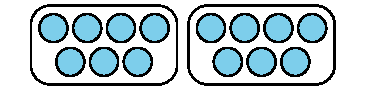
\includegraphics[width=\linewidth]{external/svg-source/tikz-file-151100.pdf}
\end{sbspanel}%
\begin{sbspanel}{0.04}%
B%
\end{sbspanel}%
\begin{sbspanel}{0.43}%
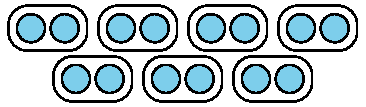
\includegraphics[width=\linewidth]{external/svg-source/tikz-file-151101.pdf}
\end{sbspanel}%
\end{sidebyside}%
\begin{sidebyside}{4}{0.0075}{0.0075}{0.015}%
\begin{sbspanel}{0.04}%
C%
\end{sbspanel}%
\begin{sbspanel}{0.43}%
\par
%
\begin{equation*}
14\div 2
\end{equation*}
%
\end{sbspanel}%
\begin{sbspanel}{0.04}%
\par
D%
\end{sbspanel}%
\begin{sbspanel}{0.43}%
\par
%
\begin{equation*}
14\div 7
\end{equation*}
%
\end{sbspanel}%
\end{sidebyside}%
\par\smallskip%
\noindent\textbf{\blocktitlefont Solución}.\hypertarget{cool-losTromposDe-3}{}\quad{}A y C%
\end{project}%
\par
\begin{paragraphs}{Posibles errores.}{cool-losTromposDe-4-1}%
Los estudiantes seleccionan respuestas que corresponden a 7 grupos de 2 en lugar de 2 grupos de 7.%
\end{paragraphs}%
\begin{paragraphs}{Acciones para apoyar el aprendizaje.}{cool-losTromposDe-4-2}%
Pida a los estudiantes al inicio de la siguiente lección que trabajen en parejas en este problema.%
\end{paragraphs}%
\end{reading-questions-subsubsection}
\end{subsectionptx}
%
%
\typeout{************************************************}
\typeout{Subsección  Lección 5 -~Escribamos expresiones de división}
\typeout{************************************************}
%
\begin{subsectionptx}{Subsección}{Lección 5 -~Escribamos expresiones de división}{}{Lección 5}{}{}{lec-escribamosExpresionesDivision}
\begin{objectives}{Objetivos de aprendizaje}{lec-escribamosExpresionesDivision-4}
%
\begin{itemize}[label=\textbullet]
\item{}Resolver problemas de "¿cuántos grupos?" y "¿cuántos en cada grupo?".%
\item{}Escribir expresiones de división para representar situaciones de división.%
\end{itemize}
\end{objectives}
\begin{introduction}{}%
\begin{paragraphs}{Estándares CCSS asociados.}{lec-escribamosExpresionesDivision-5-1}%
3.NBT.A.2, 3.OA.A.2, 3.OA.A.3%
\end{paragraphs}%
\begin{paragraphs}{Momentos de la lección.}{lec-escribamosExpresionesDivision-5-2}%
\noindent
\begin{longtable}[l]{ll}
\addtocounter{table}{-1}
\endfirsthead
\endhead
\multicolumn{2}{r}{(Continúa en la página siguiente)}\\
\endfoot
\endlastfoot
\hyperref[lec-escribamosExpresionesDivision-warm]{Subsubsección }& Calentamiento~(10 mins)\\
\hyperref[lec-escribamosExpresionesDivision-act1]{Subsubsección }& Actividad 1~(15 mins)\\
\hyperref[lec-escribamosExpresionesDivision-act2]{Subsubsección }& Actividad 2~(20 mins)\\
\hyperref[lec-escribamosExpresionesDivision-sintesis]{Subsubsección }& Síntesis de la lección~(10 mins)\\
\hyperref[lec-escribamosExpresionesDivision-cool]{Preguntas de comprensión }& Actividad de cierre~(5 mins)\\
\end{longtable}
\end{paragraphs}%
\begin{paragraphs}{Propósito de la lección.}{lec-escribamosExpresionesDivision-5-3}%
El propósito de esta lección es que los estudiantes escriban expresiones de división para representar situaciones de división y resuelvan problemas de "¿cuántos grupos?" y "¿cuántos en cada grupo?".%
\end{paragraphs}%
\begin{paragraphs}{Materiales.}{lec-escribamosExpresionesDivision-5-4}%
%
\begin{itemize}[label=\textbullet]
\item{}Actividad 1%
%
\begin{itemize}[label=$\circ$]
\item{}Un conjunto de tarjetas previamente recortadas por cada grupo de 2 estudiantes (disponibles en el libro de trabajo o \href{external/act-pdf/act-clasificacionDeTarjetas-todoSobreBichos.pdf}{descargar acá}\footnote{\nolinkurl{external/act-pdf/act-clasificacionDeTarjetas-todoSobreBichos.pdf}\label{lec-escribamosExpresionesDivision-5-4-2-1-2-1-2}})%
\end{itemize}
\item{}Actividad 2%
%
\begin{itemize}[label=$\circ$]
\item{}Herramientas para crear una presentación visual.%
\end{itemize}
\end{itemize}
\end{paragraphs}%
\begin{paragraphs}{Narrativa de la lección.}{lec-escribamosExpresionesDivision-5-5}%
Los estudiantes clasifican situaciones de división dependiendo de si el número de grupos es desconocido o si el número de objetos en cada grupo es desconocido y escriben expresiones de división para representar cada situación (MP2). Luego, los estudiantes tienen la oportunidad de usar las representaciones que han aprendido en esta sección para resolver problemas de división.%
\end{paragraphs}%
\begin{paragraphs}{Preguntas de reflexión.}{lec-escribamosExpresionesDivision-5-6}%
¿Cómo han evolucionado las estrategias de los estudiantes para resolver problemas de división desde la primera lección de esta unidad?%
\end{paragraphs}%
\end{introduction}%
%
%
\typeout{************************************************}
\typeout{Subsubsección  Calentamiento~(10 mins)}
\typeout{************************************************}
%
\begin{subsubsectionptx}{Subsubsección}{Calentamiento~(10 mins)}{}{Calentamiento}{}{}{lec-escribamosExpresionesDivision-warm}
\par
\begin{paragraphs}{Tiempo recomendado.}{warm-numTalk-enQueSeParecen-4-1}%
10 minutos%
\end{paragraphs}%
\begin{paragraphs}{Narrativa.}{warm-numTalk-enQueSeParecen-4-2}%
El propósito de esta conversación numérica es hacer visibles las estrategias y comprensiones que los estudiantes tienen para restar hasta 1,000 (es decir, sin que los números ni los resultados se pasen de 1,000), especialmente con expresiones que mantienen una diferencia constante. Estas comprensiones ayudan a desarrollar fluidez para restar con números hasta 1,000. Considere dibujar líneas numéricas mientras los estudiantes comparten sus estrategias para enfatizar que la diferencia de los dos números en cada expresión no está cambiando.%
\end{paragraphs}%
\begin{paragraphs}{Lanzamiento.}{warm-numTalk-enQueSeParecen-4-3}%
%
\begin{itemize}[label=\textbullet]
\item{}Muestre una expresión.%
\item{}``Hagan una señal cuando tengan una respuesta y puedan explicar cómo la obtuvieron.''%
\item{}1 minuto: tiempo de reflexión en silencio%
\end{itemize}
\end{paragraphs}%
\begin{paragraphs}{Desarrollo de la actividad.}{warm-numTalk-enQueSeParecen-4-4}%
%
\begin{itemize}[label=\textbullet]
\item{}Registre las respuestas y las estrategias.%
\item{}Mantenga las expresiones y el trabajo visible.%
\item{}Repita con cada expresión.%
\end{itemize}
\end{paragraphs}%
\begin{exploration}{Calentamiento}{Conversación numérica: ¿En qué se parecen?}{warm-numTalk-enQueSeParecen}%
Encuentra mentalmente el valor de cada expresión.%
\par
%
\begin{enumerate}[label={\Alph*.}]
\item{}\(\displaystyle 225 - 100\)%
\item{}\(\displaystyle 227 - 102\)%
\item{}\(\displaystyle 230 - 105\)%
\item{}\(\displaystyle 220 - 95\)%
\end{enumerate}
%
\par\smallskip%
\noindent\textbf{\blocktitlefont Solución}.\hypertarget{warm-numTalk-enQueSeParecen-3}{}\quad{}Ejemplos de respuestas%
\par
%
\begin{enumerate}[label={\Alph*.}]
\item{}125. La diferencia entre 100 y 200 es 100, entonces faltan 25 más para llegar a 225.%
\item{}125. Me di cuenta de que le sumaron 2 a los dos números del primer problema. Así que ahora son 98 para llegar a 200, y 27 más para llegar a 227. \(98+27=125\).%
\item{}125. Se le sumó 5 a cada número del primer problema, así que la diferencia entre los números sigue siendo 125.%
\item{}125. Esta vez se le restó 5 a los dos números. Le sumé 5 a 95 para llegar a 100 y 120 más para llegar a 220, entonces el valor sigue siendo 125.%
\end{enumerate}
%
\end{exploration}%
\par
\begin{paragraphs}{Síntesis de la actividad.}{warm-numTalk-enQueSeParecen-5-1}%
%
\begin{itemize}[label=\textbullet]
\item{}``¿Qué observan acerca de estas expresiones?'' (Todas tienen el mismo valor.)%
\item{}``¿Cómo podemos darnos cuenta de que todas tienen el mismo valor sin necesidad de calcular el resultado en cada caso?'' (Dado que se suma o resta la misma cantidad a ambos números de la expresión original, la diferencia no cambia.)%
\item{}Considera preguntar:%
\begin{itemize}[label=$\circ$]
\item{}``¿Alguien puede expresar el razonamiento de \fillintext{10} de otra forma?''%
\item{}``¿Alguien usó la misma estrategia, pero la explicaría de otra forma?''%
\item{}``¿Alguien pensó en el problema de otra forma?''%
\item{}``¿Alguien quiere agregar algo a la estrategia de \fillintext{10}?''%
\end{itemize}
%
\end{itemize}
\end{paragraphs}%
\end{subsubsectionptx}
%
%
\typeout{************************************************}
\typeout{Subsubsección  Actividad 1~(15 mins)}
\typeout{************************************************}
%
\begin{subsubsectionptx}{Subsubsección}{Actividad 1~(15 mins)}{}{Actividad 1}{}{}{lec-escribamosExpresionesDivision-act1}
\par
\begin{paragraphs}{Tiempo recomendado.}{act-clasificacionDeTarjetas-todoSobreBichos-4-1}%
15 minutos%
\end{paragraphs}%
\begin{paragraphs}{Narrativa.}{act-clasificacionDeTarjetas-todoSobreBichos-4-2}%
El propósito de esta actividad es que los estudiantes determinen si una situación se trata de un número desconocido de grupos o un número desconocido de objetos en cada grupo. Después de clasificar las situaciones, los estudiantes escriben una expresión de división para representar cada situación. El hecho de que la estructura de las expresiones sea la misma al representar un número desconocido de grupos o un número desconocido de objetos en cada grupo enfatiza aún más que las expresiones de división pueden interpretarse de dos maneras. Cuando los estudiantes discuten y justifican sus decisiones, comparten una afirmación matemática y el pensamiento que hay detrás de ella (MP3).%
\end{paragraphs}%
\begin{paragraphs}{Materiales.}{act-clasificacionDeTarjetas-todoSobreBichos-4-3}%
%
\begin{itemize}[label=\textbullet]
\item{}Un conjunto de tarjetas previamente recortadas por cada grupo de 2 estudiantes (disponibles en el libro de trabajo o \href{external/act-pdf/act-clasificacionDeTarjetas-todoSobreBichos.pdf}{descargar acá}\footnotemark{})%
\end{itemize}
\end{paragraphs}%
\begin{paragraphs}{Lanzamiento.}{act-clasificacionDeTarjetas-todoSobreBichos-4-4}%
%
\begin{itemize}[label=\textbullet]
\item{}Grupos de 2%
\item{}Muestre la imagen.%
\item{}``Vamos a trabajar con algunas situaciones que incluyen insectos. Los insectos son un tipo de bicho.''%
\item{}``¿Qué partes de los insectos podemos contar?'' (patas, ojos, alas, antenas, segmentos del cuerpo)%
\item{}Si es necesario, aclare qué son las antenas.%
\item{}Distribuya un conjunto de tarjetas previamente recortadas a cada grupo de estudiantes.%
\end{itemize}
\end{paragraphs}%
\begin{paragraphs}{Desarrollo de la actividad.}{act-clasificacionDeTarjetas-todoSobreBichos-4-5}%
%
\begin{itemize}[label=\textbullet]
\item{}``En esta actividad, van a clasificar algunas tarjetas en las categorías que elijan con su compañero.''%
\item{}5 minutos: tiempo de trabajo en pareja%
\item{}Seleccionar grupos para compartir sus categorías y cómo clasificaron sus tarjetas.%
\item{}Elegir tantos tipos diferentes de categorías como el tiempo lo permita, pero asegurarse de que un conjunto de categorías distinga entre problemas de "¿cuántos grupos?" y problemas de "¿cuántos hay en cada grupo?"%
\item{}Si ninguna pareja clasificó las tarjetas por tipo de situación de división, darles un minuto para hacerlo y luego discutir cómo saben qué tipo de división representa cada situación.%
\item{}``Ahora, con su compañero, clasifiquen sus tarjetas en problemas de '¿cuántos grupos?' y problemas de '¿cuántos hay en cada grupo?'?''%
\item{}``Una vez que hayan clasificado sus tarjetas, escriban una expresión de división para representar cada situación.''%
\item{}5 minutos: tiempo de trabajo en pareja%
\end{itemize}
\end{paragraphs}%
\begin{activity}{Actividad}{Clasificación de tarjetas: Todo sobre bichos.}{act-clasificacionDeTarjetas-todoSobreBichos}%
\begin{image}{0.3}{0.4}{0.3}{-1.5\baselineskip}%
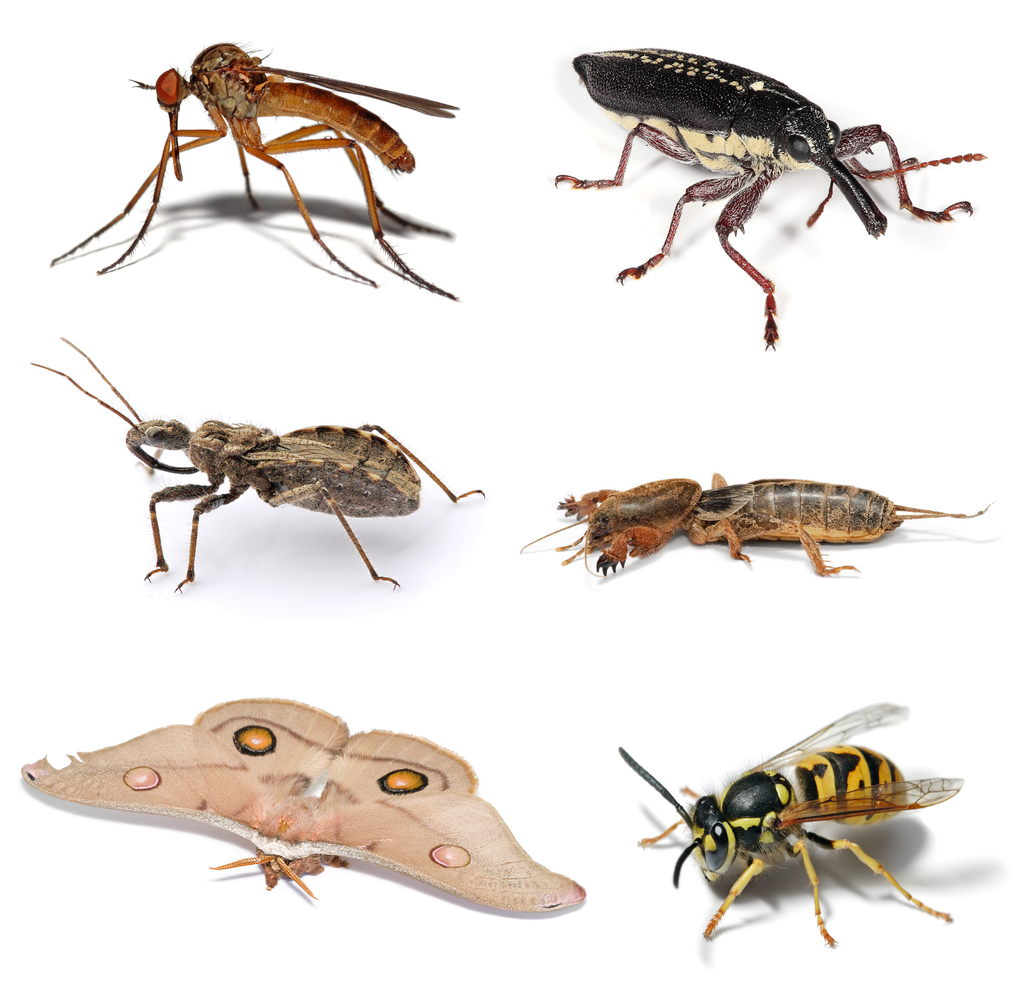
\includegraphics[width=\linewidth]{external/png-source/v1 3.4.A5 Launch.png}
\end{image}%
%
\begin{enumerate}
\item{}Tu profesor te dará un grupo de tarjetas que describen situaciones. Elige dos categorías y clasifica las tarjetas en esas dos categorías. Prepárate para explicar el significado de tus categorías.%
\item{}Escribe una expresión de división para representar cada situación. Prepárate para explicar tu razonamiento.%
\end{enumerate}
\par\smallskip%
\noindent\textbf{\blocktitlefont Solución}.\hypertarget{act-clasificacionDeTarjetas-todoSobreBichos-3}{}\quad{}%
\begin{enumerate}
\item{}Ejemplo de respuesta:%
%
\begin{enumerate}
\item{}Situaciones sobre encontrar el número de grupos: B, C, D%
\item{}Situaciones sobre encontrar el número de objetos que hay en cada grupo: A, E, F%
\end{enumerate}
\item{}Expresiones:%
\begin{enumerate}[label={\Alph*.}]
\item{}\(\displaystyle 10\div 5\)%
\item{}\(\displaystyle 8\div 2\)%
\item{}\(\displaystyle 14\div 2\)%
\item{}\(\displaystyle 14\div 4\)%
\item{}\(\displaystyle 30\div 5\)%
\item{}\(\displaystyle 50\div 5\)%
\end{enumerate}
%
\end{enumerate}
\end{activity}%
\footnotetext[33]{\nolinkurl{en.wikipedia.org/wiki/File:Insect_collage.png}\label{act-clasificacionDeTarjetas-todoSobreBichos-2-1-2-1-2}}%
\footnotetext[34]{\nolinkurl{external/act-pdf/act-clasificacionDeTarjetas-todoSobreBichos.pdf}\label{act-clasificacionDeTarjetas-todoSobreBichos-4-3-2-1-2}}%
\par
\begin{paragraphs}{Para los estudiantes con dificultades.}{act-clasificacionDeTarjetas-todoSobreBichos-5-1}%
Algunos estudiantes pueden confundirse porque no se trata de grupos de animales, sino que cada animal representa un grupo de antenas o un grupo de patas.%
\end{paragraphs}%
\begin{paragraphs}{Síntesis de la actividad.}{act-clasificacionDeTarjetas-todoSobreBichos-5-2}%
%
\begin{itemize}[label=\textbullet]
\item{}Invite a los estudiantes a compartir la expresión que escribieron para cada situación.%
\item{}Considere preguntar a los estudiantes:%
\begin{itemize}[label=$\circ$]
\item{}``¿Qué representa cada número de la expresión?''%
\item{}``¿En qué parte de la expresión ven el número de grupos?''%
\item{}``¿En qué parte de la expresión ven el número de objetos en cada grupo?''%
\end{itemize}
%
\end{itemize}
\end{paragraphs}%
\begin{paragraphs}{Desarrollo de lenguaje matemático.}{act-clasificacionDeTarjetas-todoSobreBichos-5-3}%
Apoyos para la discusión de MLR8. Síntesis. Muestre un esquema de oración para apoyar la discusión en clase: "Observamos \fillintext{10}, entonces . . . "%
\end{paragraphs}%
\end{subsubsectionptx}
%
%
\typeout{************************************************}
\typeout{Subsubsección  Actividad 2~(20 mins)}
\typeout{************************************************}
%
\begin{subsubsectionptx}{Subsubsección}{Actividad 2~(20 mins)}{}{Actividad 2}{}{}{lec-escribamosExpresionesDivision-act2}
\par
\begin{paragraphs}{Tiempo recomendado.}{act-resolvamosProblemaBichos-4-1}%
20 minutos%
\end{paragraphs}%
\begin{paragraphs}{Narrativa.}{act-resolvamosProblemaBichos-4-2}%
En esta actividad, los estudiantes consolidan su comprensión de los tipos de situaciones de división y sus representaciones para resolver problemas de división.%
\par
Durante la síntesis, organice y muestre los pósteres de los estudiantes por tipo, de acuerdo a las categorías de la actividad anterior.%
\end{paragraphs}%
\begin{paragraphs}{Materiales.}{act-resolvamosProblemaBichos-4-3}%
%
\begin{itemize}[label=\textbullet]
\item{}Herramientas para crear una presentación visual.%
\end{itemize}
\end{paragraphs}%
\begin{paragraphs}{Lanzamiento.}{act-resolvamosProblemaBichos-4-4}%
%
\begin{itemize}[label=\textbullet]
\item{}Grupos de 2%
\item{}Asigne a cada grupo uno de los problemas de la actividad anterior y pídales que lo resuelvan.%
\item{}Proporcione a cada grupo herramientas para crear una presentación visual.%
\end{itemize}
\end{paragraphs}%
\begin{paragraphs}{Desarrollo de la actividad.}{act-resolvamosProblemaBichos-4-5}%
MLR7 Comparar y Conectar. Avances: representar, conversar%
%
\begin{itemize}[label=\textbullet]
\item{}``Hagan una presentación visual que muestre cómo pensaron en el problema que les asigné. Incluyan detalles, como notas, diagramas, dibujos, etc., para ayudar a los demás a entender sus ideas.''%
\item{}``5 minutos: tiempo de trabajo en parejas''%
\item{}``8-10 minutos: recorrido por el salón''%
\end{itemize}
\end{paragraphs}%
\begin{activity}{Actividad}{Resolvamos un problema sobre bichos.}{act-resolvamosProblemaBichos}%
Tu profesor les va a asignar un problema.%
\par
Hagan una presentación visual que muestre cómo pensaron y que muestre su solución al problema.%
\par\smallskip%
\noindent\textbf{\blocktitlefont Solución}.\hypertarget{act-resolvamosProblemaBichos-3}{}\quad{}%
\begin{enumerate}[label={\Alph*.}]
\item{}2 patas especiales%
\item{}4 escarabajos%
\item{}7 abejas%
\item{}3 libélulas%
\item{}6 patas%
\item{}10 manchas%
\end{enumerate}
%
\end{activity}%
\par
\begin{paragraphs}{Síntesis de la actividad.}{act-resolvamosProblemaBichos-5-1}%
%
\begin{itemize}[label=\textbullet]
\item{}``¿En qué se parecen los dos tipos de problemas de división?'' (Ambos implican poner cosas en grupos iguales.)%
\item{}``¿En qué se diferencian?'' (A veces sabemos cuántas cosas hay en cada grupo y necesitamos encontrar cuántos grupos podemos formar. A veces sabemos cuántos grupos hay, pero necesitamos encontrar cuántas cosas hay en cada grupo.)%
\end{itemize}
\end{paragraphs}%
\begin{paragraphs}{Desarrollo de lenguaje matemático.}{act-resolvamosProblemaBichos-5-2}%
MLR7 Comparar y Conectar. Avances: representar, conversar%
\end{paragraphs}%
\end{subsubsectionptx}
%
%
\typeout{************************************************}
\typeout{Subsubsección  Síntesis de la lección~(10 mins)}
\typeout{************************************************}
%
\begin{subsubsectionptx}{Subsubsección}{Síntesis de la lección~(10 mins)}{}{Síntesis de la lección~(10 mins)}{}{}{lec-escribamosExpresionesDivision-sintesis}
Tiempo recomendado: 10 mins.%
\par
``En las últimas lecciones hemos aprendido sobre la división. Representamos y resolvimos dos tipos de problemas de división. Resumamos juntos lo que sabemos sobre la división''%
\par
``¿Cuáles son algunas de las ideas principales que hemos aprendido sobre la división?''%
\par
Ayude a los estudiantes a aproximarse a las siguientes ideas:%
\begin{itemize}[label=\textbullet]
\item{}La división es sobre \emph{grupos iguales}.%
\item{}Con la división podemos encontrar el número de grupos, o cuántos hay en cada grupo.%
\item{}Podemos representar la división haciendo dibujos y escribiendo expresiones con \(\div\).%
\end{itemize}
%
\par
Organice las ideas de la clase en un gráfico con dos columnas, con representaciones de "¿cuántos grupos?" en una columna y las de "¿cuántos en cada grupo?" en la otra (como aparece en el resumen de la sección para estudiantes).%
\end{subsubsectionptx}
%
%
\typeout{************************************************}
\typeout{Preguntas de comprensión  Actividad de cierre~(5 mins)}
\typeout{************************************************}
%
\begin{reading-questions-subsubsection}{Preguntas de comprensión}{Actividad de cierre~(5 mins)}{}{Actividad de cierre}{}{}{lec-escribamosExpresionesDivision-cool}
\href{external/cools-pdf/cool-patasHormigas-standalone.pdf}{Descargar pdf para imprimir o proyectar}\footnote{\nolinkurl{external/cools-pdf/cool-patasHormigas-standalone.pdf}\label{lec-escribamosExpresionesDivision-cool-5}}\begin{project}{Actividad de cierre}{Patas de hormigas.}{cool-patasHormigas}%
En una fila de 4 hormigas se contaron veinticuatro patas. Todas las hormigas tienen el mismo número de patas.%
\par
%
\begin{enumerate}[label={(\alph*)}]
\item{}Escribe una expresión de división que represente esta situación.%
\item{}¿Cuántas patas tiene cada hormiga? Explica o muestra tu razonamiento.%
\end{enumerate}
%
\par\smallskip%
\noindent\textbf{\blocktitlefont Solución}.\hypertarget{cool-patasHormigas-3}{}\quad{}%
\begin{enumerate}[label={(\alph*)}]
\item{}\(\displaystyle 24\div 4\)%
\item{}6 patas. Ejemplo de respuesta: Un dibujo de 4 grupos de 6.%
\end{enumerate}
%
\end{project}%
\par
\begin{paragraphs}{Posibles errores.}{cool-patasHormigas-4-1}%
Los estudiantes escriben una expresión distinta a ``24 \textbackslash{}div 4'' para que se ajuste a la situación o no encuentran una solución al problema.%
\end{paragraphs}%
\begin{paragraphs}{Acciones para apoyar el aprendizaje.}{cool-patasHormigas-4-2}%
Pida a los estudiantes al inicio de la siguiente lección que trabajen en parejas en este problema.%
\end{paragraphs}%
\end{reading-questions-subsubsection}
\end{subsectionptx}
%
%
\typeout{************************************************}
\typeout{Ejercicios  Problemas de práctica de la sección A}
\typeout{************************************************}
%
\begin{exercises-subsection}{Ejercicios}{Problemas de práctica de la sección A}{}{Problemas de práctica}{}{}{gra3-uni4-secA-ProblemasPractica}
\begin{divisionexercise}{1}{(Previo a la sección).}{}{gra3-uni4-secA-ProblemasPractica-3}%
\begin{sidebyside}{2}{0}{0}{0}%
\begin{sbspanel}{0.3}%
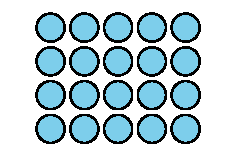
\includegraphics[width=\linewidth]{external/svg-source/tikz-file-151668.pdf}
\end{sbspanel}%
\begin{sbspanel}{0.7}%
%
\begin{enumerate}[label={(\alph*)}]
\item{}Escribe una expresión de multiplicación que represente el arreglo.%
\item{}Escribe una ecuación de multiplicación que represente el arreglo.%
\end{enumerate}
%
\end{sbspanel}%
\end{sidebyside}%
\par\smallskip%
\noindent\textbf{\blocktitlefont Solución}.\hypertarget{gra3-uni4-secA-ProblemasPractica-3-3}{}\quad{}Ejemplos de respuestas:%
%
\begin{enumerate}[label={(\alph*)}]
\item{}\(4\times 5\) o \(5\times 4\)%
\item{}\(4\times 5=20\) o \(5\times 4=20\)%
\end{enumerate}
\end{divisionexercise}%
\begin{divisionexercise}{2}{(Previo a la sección).}{}{gra3-uni4-secA-ProblemasPractica-4}%
Encuentra el área de cada rectángulo.%
\begin{sidebyside}{2}{0.05}{0.05}{0.1}%
\begin{sbspanel}{0.3}%
A.%
\par
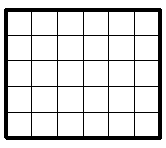
\includegraphics[width=\linewidth]{external/svg-source/tikz-file-151669-scale13.pdf}
\end{sbspanel}%
\begin{sbspanel}{0.5}%
B.%
\par
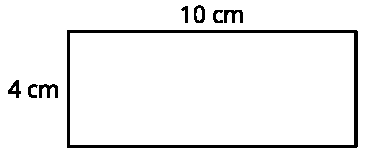
\includegraphics[width=\linewidth]{external/svg-source/tikz-file-151670-scale13.pdf}
\end{sbspanel}%
\end{sidebyside}%
\par\smallskip%
\noindent\textbf{\blocktitlefont Solución}.\hypertarget{gra3-uni4-secA-ProblemasPractica-4-3}{}\quad{}Ejemplos de respuestas%
%
\begin{enumerate}[label={\Alph*.}]
\item{}30 unidades cuadradas%
\item{}40 centímetros cuadrados.%
\end{enumerate}
\end{divisionexercise}%
\begin{divisionexercise}{3}{(Previo a la sección).}{}{gra3-uni4-secA-ProblemasPractica-5}%
El área del rectángulo es 40 centímetros cuadrados.%
\begin{sidebyside}{2}{0}{0}{0}%
\begin{sbspanel}{0.5}%
Encuentra la longitud de lado desconocida del rectángulo. Explica tu razonamiento.%
\end{sbspanel}%
\begin{sbspanel}{0.5}%
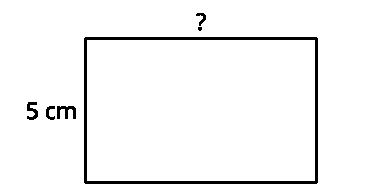
\includegraphics[width=\linewidth]{external/svg-source/tikz-file-151673-scale13.pdf}
\end{sbspanel}%
\end{sidebyside}%
\par\smallskip%
\noindent\textbf{\blocktitlefont Solución}.\hypertarget{gra3-uni4-secA-ProblemasPractica-5-3}{}\quad{}8 cm. Respuesta de muestra: Sé que \(5 \times 8 = 40\)%
\end{divisionexercise}%
\begin{divisionexercise}{4}{(Previo a la sección).}{}{gra3-uni4-secA-ProblemasPractica-6}%
En cada caso, encuentra el número que hace que la ecuación sea verdadera.%
\par
%
\begin{enumerate}[label={(\alph*)}]
\item{}\(\displaystyle 8 \times 5 = \underline{\hspace{1cm}}\)%
\item{}\(\displaystyle 5 \times \underline{\hspace{1cm}} = 35\)%
\item{}\(\displaystyle \underline{\hspace{1cm}} \times 2 = 18\)%
\end{enumerate}
%
\par\smallskip%
\noindent\textbf{\blocktitlefont Solución}.\hypertarget{gra3-uni4-secA-ProblemasPractica-6-3}{}\quad{}%
\begin{enumerate}[label={(\alph*)}]
\item{}40%
\item{}7%
\item{}9%
\end{enumerate}
\end{divisionexercise}%
\begin{divisionexercise}{5}{(Previo a la sección).}{}{gra3-uni4-secA-ProblemasPractica-7}%
Hay 6 equipos de voleibol en el gimnasio. Cada equipo tiene 10 jugadores. ¿Cuántos jugadores de voleibol hay en total?%
\par
%
\begin{enumerate}[label={(\alph*)}]
\item{}Haz un dibujo de la situación.%
\item{}Escribe una ecuación que represente la situación. Usa un “?” para representar el valor desconocido.%
\item{}Resuelve el problema.%
\end{enumerate}
%
\par\smallskip%
\noindent\textbf{\blocktitlefont Solución}.\hypertarget{gra3-uni4-secA-ProblemasPractica-7-3}{}\quad{}%
\begin{enumerate}[label={(\alph*)}]
\item{}Los estudiantes dibujan 6 grupos de 10.%
\item{}\(6 \times 10 = {?}\) o \(10 \times 6 = {?}\)%
\item{}Hay 60 jugadores de voleibol en los 6 equipos.%
\end{enumerate}
\end{divisionexercise}%
\begin{divisionexercise}{6}{}{}{gra3-uni4-secA-ProblemasPractica-8}%
En cada problema, usa un dibujo o un diagrama para mostrar cómo pensaste.%
\par
%
\begin{enumerate}[label={(\alph*)}]
\item{}Hay 40 manzanas empacadas en cajas. Si hay 8 manzanas en cada caja, ¿cuántas cajas hay?%
\item{}Hay 40 manzanas empacadas en cajas. Si hay 10 manzanas en cada caja, ¿cuántas cajas hay?%
\end{enumerate}
%
\par\smallskip%
\noindent\textbf{\blocktitlefont Solución}.\hypertarget{gra3-uni4-secA-ProblemasPractica-8-2}{}\quad{}%
\begin{enumerate}[label={(\alph*)}]
\item{}5. Ejemplo de respuesta%
\begin{image}{0}{1}{0}{}%
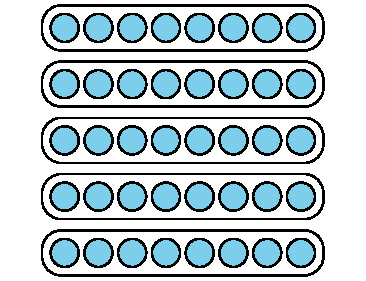
\includegraphics[width=\linewidth]{external/svg-source/tikz-file-152430.pdf}
\end{image}%
\item{}4. Ejemplo de respuesta%
\begin{image}{0}{1}{0}{}%
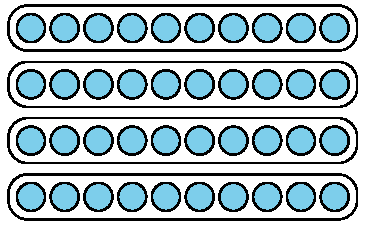
\includegraphics[width=\linewidth]{external/svg-source/tikz-file-152431.pdf}
\end{image}%
\end{enumerate}
\end{divisionexercise}%
\begin{divisionexercise}{7}{}{}{gra3-uni4-secA-ProblemasPractica-9}%
En cada problema, usa un dibujo o un diagrama para mostrar cómo pensaste.%
%
\begin{enumerate}[label={(\alph*)}]
\item{}Hay 30 naranjas. Las empacan en 5 bolsas. Si hay la misma cantidad de naranjas en cada bolsa, ¿cuántas naranjas hay en cada bolsa?%
\item{}Hay 30 naranjas. Las empacan en 3 bolsas. Si hay la misma cantidad de naranjas en cada bolsa, ¿cuántas naranjas hay en cada bolsa?%
\end{enumerate}
\par\smallskip%
\noindent\textbf{\blocktitlefont Solución}.\hypertarget{gra3-uni4-secA-ProblemasPractica-9-2}{}\quad{}%
\begin{enumerate}[label={(\alph*)}]
\item{}6. Ejemplo de respuesta%
\begin{image}{0}{1}{0}{}%
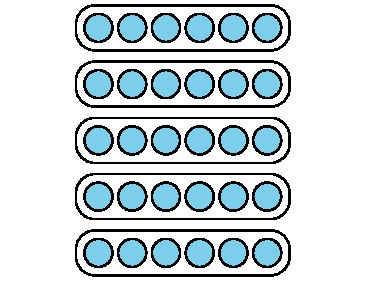
\includegraphics[width=\linewidth]{external/svg-source/tikz-file-152432.pdf}
\end{image}%
\item{}10. Ejemplo de respuesta%
\begin{image}{0}{1}{0}{}%
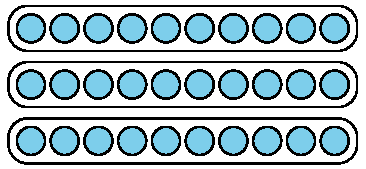
\includegraphics[width=\linewidth]{external/svg-source/tikz-file-152433.pdf}
\end{image}%
\end{enumerate}
\end{divisionexercise}%
\begin{divisionexercise}{8}{}{}{gra3-uni4-secA-ProblemasPractica-10}%
%
\begin{enumerate}[label={(\alph*)}]
\item{}10 personas van a cine en automóviles. En cada automóvil van dos personas. ¿Cuántos automóviles hay? Muestra cómo pensaste. Usa un dibujo o un diagrama.%
\item{}Otras 10 personas van a cine en automóviles. Van en 2 automóviles con el mismo número de personas en cada automóvil. ¿Cuántas personas hay en cada automóvil? Muestra cómo pensaste. Usa un dibujo o un diagrama.%
\item{}¿En qué se parecen las dos situaciones? ¿En qué son diferentes? ¿En qué se parecen los diagramas? ¿En qué son diferentes?%
\end{enumerate}
%
\par\smallskip%
\noindent\textbf{\blocktitlefont Solución}.\hypertarget{gra3-uni4-secA-ProblemasPractica-10-2}{}\quad{}%
\begin{enumerate}[label={(\alph*)}]
\item{}5.%
\begin{image}{0}{1}{0}{}%
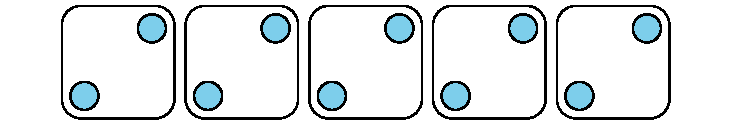
\includegraphics[width=\linewidth]{external/svg-source/tikz-file-152434.pdf}
\end{image}%
\item{}10. Ejemplo de respuesta%
\begin{image}{0}{1}{0}{}%
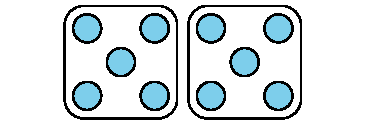
\includegraphics[width=\linewidth]{external/svg-source/tikz-file-152435.pdf}
\end{image}%
\item{}Ejemplo de respuesta: En ambas situaciones aparecen las mismas cantidades: 2, 5 y 10. En la primera, 2 es el número de personas en cada automóvil. En la segunda, 2 es el número de automóviles.%
\end{enumerate}
\end{divisionexercise}%
\begin{divisionexercise}{9}{}{}{gra3-uni4-secA-ProblemasPractica-11}%
Hay 20 pupitres en la clase. Están divididos equitativamente en 5 grupos (es decir, la misma cantidad de pupitres en cada grupo). ¿Cuántos pupitres hay en cada grupo?%
\par
%
\begin{enumerate}[label={(\alph*)}]
\item{}¿Cuál expresión representa esta situación: \(20\div 4\) o \(20\div 5\)? Explica tu razonamiento.%
\item{}Selecciona el diagrama que representa esta situación. Explica tu razonamiento.%
\begin{sidebyside}{2}{0}{0}{0}%
\begin{sbspanel}{0.07}%
A%
\end{sbspanel}%
\begin{sbspanel}{0.93}%
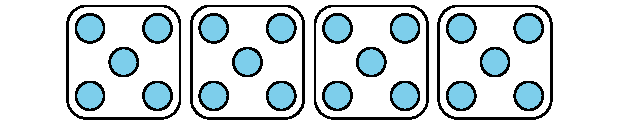
\includegraphics[width=\linewidth]{external/svg-source/tikz-file-151671.pdf}
\end{sbspanel}%
\end{sidebyside}%
\begin{sidebyside}{2}{0}{0}{0}%
\begin{sbspanel}{0.07}%
B%
\end{sbspanel}%
\begin{sbspanel}{0.93}%
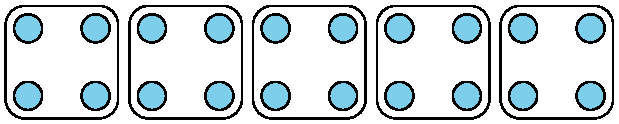
\includegraphics[width=\linewidth]{external/svg-source/tikz-file-151672.pdf}
\end{sbspanel}%
\end{sidebyside}%
\end{enumerate}
%
\par\smallskip%
\noindent\textbf{\blocktitlefont Solución}.\hypertarget{gra3-uni4-secA-ProblemasPractica-11-2}{}\quad{}%
\begin{enumerate}[label={(\alph*)}]
\item{}\(20 \div 5\), porque hay 20 pupitres divididos en 5 grupos iguales. La respuesta \(20 \div 4\) también es válida, porque hay 4 pupitres en cada grupo.%
\item{}El segundo diagrama, porque muestra 20 dividido en 5 grupos iguales.%
\end{enumerate}
\end{divisionexercise}%
\begin{divisionexercise}{10}{}{}{gra3-uni4-secA-ProblemasPractica-12}%
Los papás de Mai recolectaron 40 libras de duraznos y los pusieron en bolsas. Pusieron 5 libras en cada bolsa.%
\par
%
\begin{enumerate}[label={(\alph*)}]
\item{}Escribe una expresión de división que represente la situación.%
\item{}¿Cuántas bolsas de duraznos necesitaron los papás de Mai? Explica o muestra tu razonamiento.%
\end{enumerate}
%
\par\smallskip%
\noindent\textbf{\blocktitlefont Solución}.\hypertarget{gra3-uni4-secA-ProblemasPractica-12-2}{}\quad{}%
\begin{enumerate}[label={(\alph*)}]
\item{}\(\displaystyle 40 \div 5\)%
\item{}8. Ejemplo de respuesta:%
\begin{image}{0}{1}{0}{}%
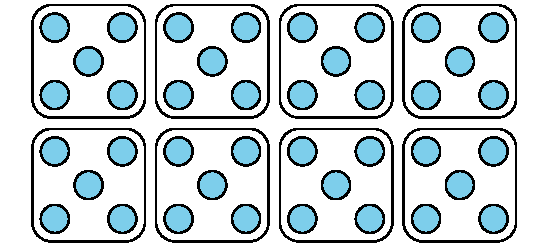
\includegraphics[width=\linewidth]{external/svg-source/tikz-file-152436.pdf}
\end{image}%
\end{enumerate}
\end{divisionexercise}%
\begin{divisionexercise}{11}{Exploración.}{}{gra3-uni4-secA-ProblemasPractica-13}%
Completa cada historia poniendo un número que tenga sentido en el espacio en blanco. Después, responde las preguntas. Dibuja un diagrama para resolver cada problema.%
\par
%
\begin{enumerate}[label={(\alph*)}]
\item{}Mai tiene \textunderscore{}\textunderscore{}\textunderscore{}\textunderscore{}\textunderscore{}\textunderscore{}\textunderscore{}\textunderscore{}\textunderscore{}\textunderscore{} calcomanías. Ella va a poner el mismo número de calcomanías en cada uno de sus 5 cuadernos. ¿Cuántas calcomanías habrá en cada cuaderno?%
\item{}Andre tiene \textunderscore{}\textunderscore{}\textunderscore{}\textunderscore{}\textunderscore{}\textunderscore{}\textunderscore{}\textunderscore{}\textunderscore{}\textunderscore{} tarjetas. Él va a organizarlas en filas de \textunderscore{}\textunderscore{}\textunderscore{}\textunderscore{}\textunderscore{}\textunderscore{}\textunderscore{}\textunderscore{}\textunderscore{}\textunderscore{} tarjetas. ¿Cuántas filas de tarjetas hará Andre?%
\end{enumerate}
%
\par\smallskip%
\noindent\textbf{\blocktitlefont Solución}.\hypertarget{gra3-uni4-secA-ProblemasPractica-13-3}{}\quad{}Ejemplos de respuestas:%
%
\begin{enumerate}[label={(\alph*)}]
\item{}30. Si Mai tiene 30 calcmanías, puede poner 6 calcomanías en cada uno de sus 5 cuadernos.%
\begin{image}{0}{1}{0}{}%
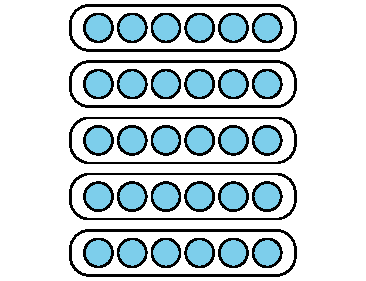
\includegraphics[width=\linewidth]{external/svg-source/tikz-file-152437.pdf}
\end{image}%
\item{}48 y 8. Si Andre tiene 48 tarjetas y organiza filas de 8 tarjetas, hará 6 filas en total.%
\begin{image}{0}{1}{0}{}%
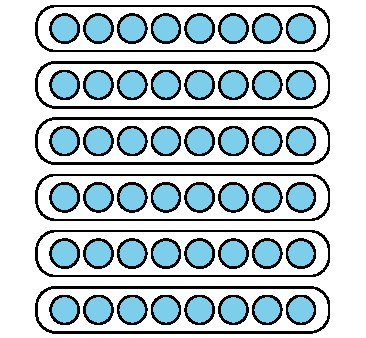
\includegraphics[width=\linewidth]{external/svg-source/tikz-file-152438.pdf}
\end{image}%
\end{enumerate}
\end{divisionexercise}%
\begin{divisionexercise}{12}{Exploración.}{}{gra3-uni4-secA-ProblemasPractica-14}%
Escribe una situación de división que corresponda a cada diagrama.%
\begin{sidebyside}{3}{0}{0}{0.02}%
\begin{sbspanel}{0.32}%
A%
\par
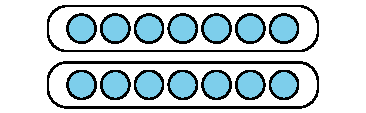
\includegraphics[width=\linewidth]{external/svg-source/tikz-file-151674.pdf}
\end{sbspanel}%
\begin{sbspanel}{0.32}%
B%
\par
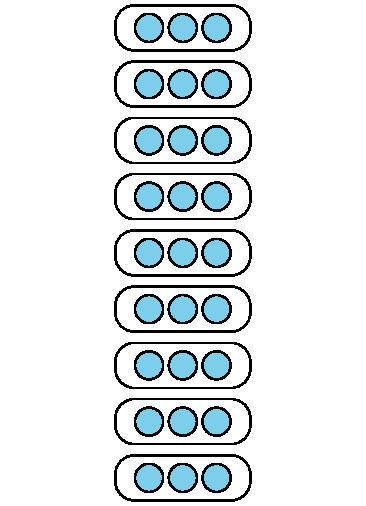
\includegraphics[width=\linewidth]{external/svg-source/tikz-file-151675.pdf}
\end{sbspanel}%
\begin{sbspanel}{0.32}%
C%
\par
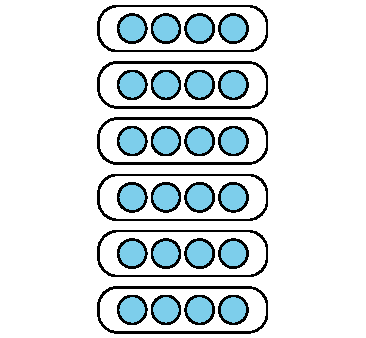
\includegraphics[width=\linewidth]{external/svg-source/tikz-file-151676.pdf}
\end{sbspanel}%
\end{sidebyside}%
\par\smallskip%
\noindent\textbf{\blocktitlefont Solución}.\hypertarget{gra3-uni4-secA-ProblemasPractica-14-3}{}\quad{}Ejemplos de repuestas:%
%
\begin{enumerate}[label={\Alph*.}]
\item{}En una caja hay 14 peras organizadas en 2 filas iguales. ¿Cuántas peras hay en cada fila?%
\item{}En la clase hay 27 estudiantes y están organizados en grupos de 3. ¿Cuántos grupos hay?%
\item{}Lin reparte 24 tarjetas entre 6 personas de manera que cada una tenga la misma cantidad de tarjetas. ¿Cuántas tarjetas recibe cada persona?%
\end{enumerate}
\end{divisionexercise}%
\end{exercises-subsection}
%
%
\typeout{************************************************}
\typeout{Referencias  Resumen de la sección~(para los estudiantes)}
\typeout{************************************************}
%
\begin{references-subsection}{Referencias}{Resumen de la sección~(para los estudiantes)}{}{Resumen sección~(estudiantes)}{}{}{gra3-uni4-secA-resumen}
En esta sección, aprendimos que la división se usa para encontrar el número de grupos o encontrar el tamaño de cada grupo cuando ponemos objetos en grupos de igual tamaño. Representamos situaciones de división con dibujos y expresiones, y resolvimos problemas de división.%
\begin{sidebyside}{2}{0.025}{0.025}{0.05}%
\begin{sbspanel}{0.45}%
``¿Cuántos grupos?''%
\end{sbspanel}%
\begin{sbspanel}{0.45}%
\par
``¿Cuántos hay en cada grupo?''%
\end{sbspanel}%
\end{sidebyside}%
\begin{sidebyside}{2}{0.025}{0.025}{0.05}%
\begin{sbspanel}{0.45}%
Han tiene 12 lápices de colores. Él quiere ponerlos en cajas. Quiere poner 2 lápices en cada caja hasta que se le acaben los lápices. ¿Cuántas cajas necesita Han?%
\end{sbspanel}%
\begin{sbspanel}{0.45}%
\par
Elena tiene 12 lápices de colores. Ella tiene 2 cajas y quiere poner el mismo número de lápices en cada caja. ¿Cuántos lápices habrá en cada caja?%
\end{sbspanel}%
\end{sidebyside}%
\begin{sidebyside}{2}{0.025}{0.025}{0.05}%
\begin{sbspanel}{0.45}%
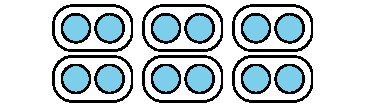
\includegraphics[width=\linewidth]{external/svg-source/tikz-file-147695.pdf}
\end{sbspanel}%
\begin{sbspanel}{0.45}%
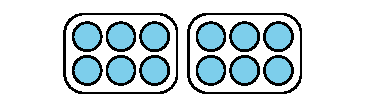
\includegraphics[width=\linewidth]{external/svg-source/tikz-file-147696.pdf}
\end{sbspanel}%
\end{sidebyside}%
\begin{sidebyside}{2}{0.025}{0.025}{0.05}%
\begin{sbspanel}{0.45}%
%
\begin{equation*}
12 \div 2
\end{equation*}
%
\end{sbspanel}%
\begin{sbspanel}{0.45}%
\par
%
\begin{equation*}
12 \div 2
\end{equation*}
%
\end{sbspanel}%
\end{sidebyside}%
\end{references-subsection}
\end{sectionptx}
%
%
\typeout{************************************************}
\typeout{Sección  Sección B -~Relacionemos la multiplicación y la división}
\typeout{************************************************}
%
\begin{sectionptx}{Sección}{Sección B -~Relacionemos la multiplicación y la división}{}{Sección B -~Relacionemos la multiplicación y la división}{}{}{gra3-uni4-secB}
\begin{introduction}{}%
\begin{objectives}{Objetivos de aprendizaje}{gra3-uni4-secB-intro-1}
%
\begin{itemize}[label=\textbullet]
\item{}Entender la división como un problema de factor desconocido.%
\item{}Usar las propiedades de las operaciones para desarrollar fluidez con hechos de multiplicación de un dígito y sus hechos de división asociados.%
\end{itemize}
\end{objectives}
En esta sección, los estudiantes relacionan de manera explícita la división con el factor desconocido en una ecuación de multiplicación. Por ejemplo, el cociente de \(30 \div 6 = \underline{\hspace{1 cm}}\) es el factor desconocido en \(\underline{\hspace{1 cm}} \times 6 = 30\). Utilizan esta idea y su conocimiento de los hechos de multiplicación para identificar los hechos de división.%
\par
Para desarrollar fluidez, los estudiantes razonan sobre patrones en una tabla de multiplicar y notan que la multiplicación es conmutativa. Por ejemplo, si ellos saben el valor de \(4 \times 7\), también saben el de \(7 \times 4\).%
\par
Además, los estudiantes razonan sobre el producto de dos factores descomponiendo uno de los dos factores. Por ejemplo, para encontrar el valor de \(7 \times 3\), ellos pueden descomponer el \(7\) en \(5\) y \(2\) y encontrar el valor de \((5 \times 3) + (2 \times 3)\). Visualmente, el producto se puede representar como el área de un rectángulo de \(7\) por \(3\) que se descompuso en dos rectángulos de \(5\) por \(3\) y \(2\) por \(3\).%
\begin{image}{0}{1}{0}{}%
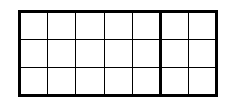
\includegraphics[width=\linewidth]{external/svg-source/tikz-file-147474.pdf}
\end{image}%
Este razonamiento desarrolla la intución de los estudiantes sobre la propiedad distributiva de la multiplicación. (Note que no se espera que los estudiantes conozcan los nombres de las propiedades de las operaciones.)%
\end{introduction}%
%
%
\typeout{************************************************}
\typeout{Subsección  Lección 6 -~La división como un factor desconocido}
\typeout{************************************************}
%
\begin{subsectionptx}{Subsección}{Lección 6 -~La división como un factor desconocido}{}{Lección 6}{}{}{lec-divisionComoFactorDesconocido}
\begin{objectives}{Objetivos de aprendizaje}{lec-divisionComoFactorDesconocido-4}
%
\begin{itemize}[label=\textbullet]
\item{}Explicar la relación entre ecuaciones de multiplicación y ecuaciones de división.%
\item{}Interpretar ecuaciones de división y ecuaciones de multiplicación que incluyan un factor desconocido.%
\end{itemize}
\end{objectives}
\begin{introduction}{}%
\begin{paragraphs}{Estándares CCSS asociados.}{lec-divisionComoFactorDesconocido-5-1}%
3.OA.A.2, 3.OA.B.6%
\end{paragraphs}%
\begin{paragraphs}{Momentos de la lección.}{lec-divisionComoFactorDesconocido-5-2}%
\noindent
\begin{longtable}[l]{ll}
\addtocounter{table}{-1}
\endfirsthead
\endhead
\multicolumn{2}{r}{(Continúa en la página siguiente)}\\
\endfoot
\endlastfoot
\hyperref[lec-divisionComoFactorDesconocido-warm]{Subsubsección }& Calentamiento~(10 mins)\\
\hyperref[lec-divisionComoFactorDesconocido-act1]{Subsubsección }& Actividad 1~(15 mins)\\
\hyperref[lec-divisionComoFactorDesconocido-act2]{Subsubsección }& Actividad 2~(20 mins)\\
\hyperref[lec-divisionComoFactorDesconocido-sintesis]{Subsubsección }& Síntesis de la lección~(10 mins)\\
\hyperref[lec-divisionComoFactorDesconocido-cool]{Preguntas de comprensión }& Actividad de cierre~(5 mins)\\
\end{longtable}
\end{paragraphs}%
\begin{paragraphs}{Propósito de la lección.}{lec-divisionComoFactorDesconocido-5-3}%
El propósito de esta lección es que los estudiantes relacionen la multiplicación y la división y reconozcan que la división es equivalente a un problema de factor desconocido.%
\end{paragraphs}%
\begin{paragraphs}{Materiales.}{lec-divisionComoFactorDesconocido-5-4}%
%
\begin{itemize}[label=\textbullet]
\item{}Actividad 2%
%
\begin{itemize}[label=$\circ$]
\item{}Tabla para rellenar. Una tabla para cada pareja (disponible en el libro de trabajo o \href{external/act-pdf/act-enElMercadoAgricola.pdf}{descargar para imprimir}\footnote{\nolinkurl{external/act-pdf/act-enElMercadoAgricola.pdf}\label{lec-divisionComoFactorDesconocido-5-4-2-1-2-1-2}}).%
\end{itemize}
\end{itemize}
\end{paragraphs}%
\begin{paragraphs}{Narrativa de la lección.}{lec-divisionComoFactorDesconocido-5-5}%
Anteriormente, los estudiantes aprendieron a interpretar y escribir expresiones de división. Conectaron la división con la multiplicación de manera informal, reconociendo que ambas operaciones involucraban grupos iguales. En esta lección, los estudiantes analizan ecuaciones relacionadas de multiplicación y división para formalizar la relación entre la multiplicación y la división. En la síntesis de la lección, los estudiantes aprenden que el resultado en una ecuación de división se llama \terminology{cociente}.%
\end{paragraphs}%
\begin{paragraphs}{Preguntas de reflexión.}{lec-divisionComoFactorDesconocido-5-6}%
En esta lección, los estudiantes relacionan por primera vez la multiplicación y la división de manera formal. ¿Cómo les está ayudando su conocimiento previo de estas operaciones a comprender esta relación?%
\end{paragraphs}%
\end{introduction}%
%
%
\typeout{************************************************}
\typeout{Subsubsección  Calentamiento~(10 mins)}
\typeout{************************************************}
%
\begin{subsubsectionptx}{Subsubsección}{Calentamiento~(10 mins)}{}{Calentamiento}{}{}{lec-divisionComoFactorDesconocido-warm}
\par
\begin{paragraphs}{Tiempo recomendado.}{warm-observa-numerosDesconocidos-4-1}%
10 minutos%
\end{paragraphs}%
\begin{paragraphs}{Narrativa.}{warm-observa-numerosDesconocidos-4-2}%
El propósito de esta actividad de calentamiento es generar la idea de que la multiplicación y la división están relacionadas, lo cual le ayudará más adelante a los estudiantes a entender que la división es como un problema de factor desconocido. Aunque los estudiantes pueden observar y preguntarse muchas cosas sobre estas ecuaciones, las ideas sobre cómo la multiplicación y la división se parecen y se diferencian son los puntos importantes en la discusión.%
\par
Los estudiantes han visto expresiones de división, pero esta será la primera vez que vean ecuaciones de división.%
\end{paragraphs}%
\begin{paragraphs}{Lanzamiento.}{warm-observa-numerosDesconocidos-4-3}%
%
\begin{itemize}[label=\textbullet]
\item{}Grupos de 2%
\item{}Mostrar las ecuaciones.%
\item{}``¿Qué observan? ¿Qué se preguntan?''%
\item{}1 minuto: tiempo para pensar en silencio%
\end{itemize}
\end{paragraphs}%
\begin{paragraphs}{Desarrollo de la actividad.}{warm-observa-numerosDesconocidos-4-4}%
%
\begin{itemize}[label=\textbullet]
\item{}``Discutan con su compañero lo que pensaron''%
\item{}1 minuto: discusión con el compañero%
\item{}Compartir y registrar respuestas.%
\end{itemize}
\end{paragraphs}%
\begin{exploration}{Calentamiento}{Observa y pregúntate: Números desconocidos.}{warm-observa-numerosDesconocidos}%
¿Qué observas?\\
 ¿Qué te preguntas?%
\begin{sidebyside}{2}{0}{0}{0}%
\begin{sbspanel}{0.5}%
%
\begin{equation*}
3\times {?} =12
\end{equation*}
%
\end{sbspanel}%
\begin{sbspanel}{0.5}%
\par
%
\begin{equation*}
12\div 3 ={?}
\end{equation*}
%
\end{sbspanel}%
\end{sidebyside}%
\par\smallskip%
\noindent\textbf{\blocktitlefont Solución}.\hypertarget{warm-observa-numerosDesconocidos-3}{}\quad{}Los estudiantes pueden notar que:%
%
\begin{itemize}[label=\textbullet]
\item{}El 12 se está dividiendo en 3 grupos de igual tamaño o en grupos de 3.%
\item{}Ambas ecuaciones tienen un 3, un 12 y un signo de interrogación, pero no están en los mismos lugares.%
\item{}Poner un 4 en el lugar del signo de interrogación tendría sentido en ambas ecuaciones.%
\end{itemize}
Los estudiantes pueden preguntarse:%
%
\begin{itemize}[label=\textbullet]
\item{}¿Es el número desconocido el mismo en ambas ecuaciones?%
\item{}¿Cuál es el número desconocido?%
\item{}¿Están relacionadas las dos ecuaciones?%
\end{itemize}
\end{exploration}%
\par
\begin{paragraphs}{Síntesis de la actividad.}{warm-observa-numerosDesconocidos-5-1}%
%
\begin{itemize}[label=\textbullet]
\item{}``Hoy vamos a seguir trabajando con ecuaciones de multiplicación y ecuaciones de división como estas''%
\end{itemize}
\end{paragraphs}%
\end{subsubsectionptx}
%
%
\typeout{************************************************}
\typeout{Subsubsección  Actividad 1~(15 mins)}
\typeout{************************************************}
%
\begin{subsubsectionptx}{Subsubsección}{Actividad 1~(15 mins)}{}{Actividad 1}{}{}{lec-divisionComoFactorDesconocido-act1}
\par
\begin{paragraphs}{Tiempo recomendado.}{act-ecuacionesCebollas-4-1}%
15 minutos%
\end{paragraphs}%
\begin{paragraphs}{Narrativa.}{act-ecuacionesCebollas-4-2}%
El propósito de esta actividad es que los estudiantes formalicen la relación entre las ecuaciones de multiplicación y las de división. Deben identificar que la cantidad desconocida en una situación de división (que más adelante aprenderán a llamar cociente) se puede representar como un factor desconocido en una ecuación de multiplicación. En la síntesis de la actividad se debe enfatizar que ambas ecuaciones son formas apropiadas de representar una situación que involucra grupos iguales.%
\par
Esta actividad brinda a los estudiantes la oportunidad de dar sentido a cada cantidad y cómo se relaciona con la situación (MP2). A medida que los estudiantes discuten y justifican sus decisiones, comparten una afirmación matemática y el razonamiento que hay detrás de ella (MP3).%
\end{paragraphs}%
\begin{paragraphs}{Lanzamiento.}{act-ecuacionesCebollas-4-3}%
%
\begin{itemize}[label=\textbullet]
\item{}Grupos de 2%
\item{}``¿En qué lugares conseguimos alimentos?''%
\item{}30 segundos: tiempo para pensar en silencio%
\item{}Compartir respuestas.%
\item{}``Esta situación se trata de conseguir alimentos en un mercado agrícola. Los mercados agrícolas son lugares donde la gente de la comunidad se reúne y vende los alimentos que ha cultivado o preparado''%
\end{itemize}
\end{paragraphs}%
\begin{paragraphs}{Desarrollo de la actividad.}{act-ecuacionesCebollas-4-4}%
%
\begin{itemize}[label=\textbullet]
\item{}``Lean cómo piensan Lin y Mai acerca de esta situación y decidan con quién están de acuerdo y por qué''%
\item{}3 minutos: tiempo de trabajo individual%
\item{}Identifique qué estudiantes están de acuerdo con qué ecuaciones y emparéjelos para la discusión.%
\item{}3 minutos: discusión en parejas%
\item{}Identifique a los estudiantes que puedan articular por qué tanto Lin como Mai tienen razón.%
\end{itemize}
\end{paragraphs}%
\begin{activity}{Actividad}{Ecuaciones acerca de cebollas.}{act-ecuacionesCebollas}%
\begin{image}{0.15}{0.7}{0.15}{-1.5\baselineskip}%
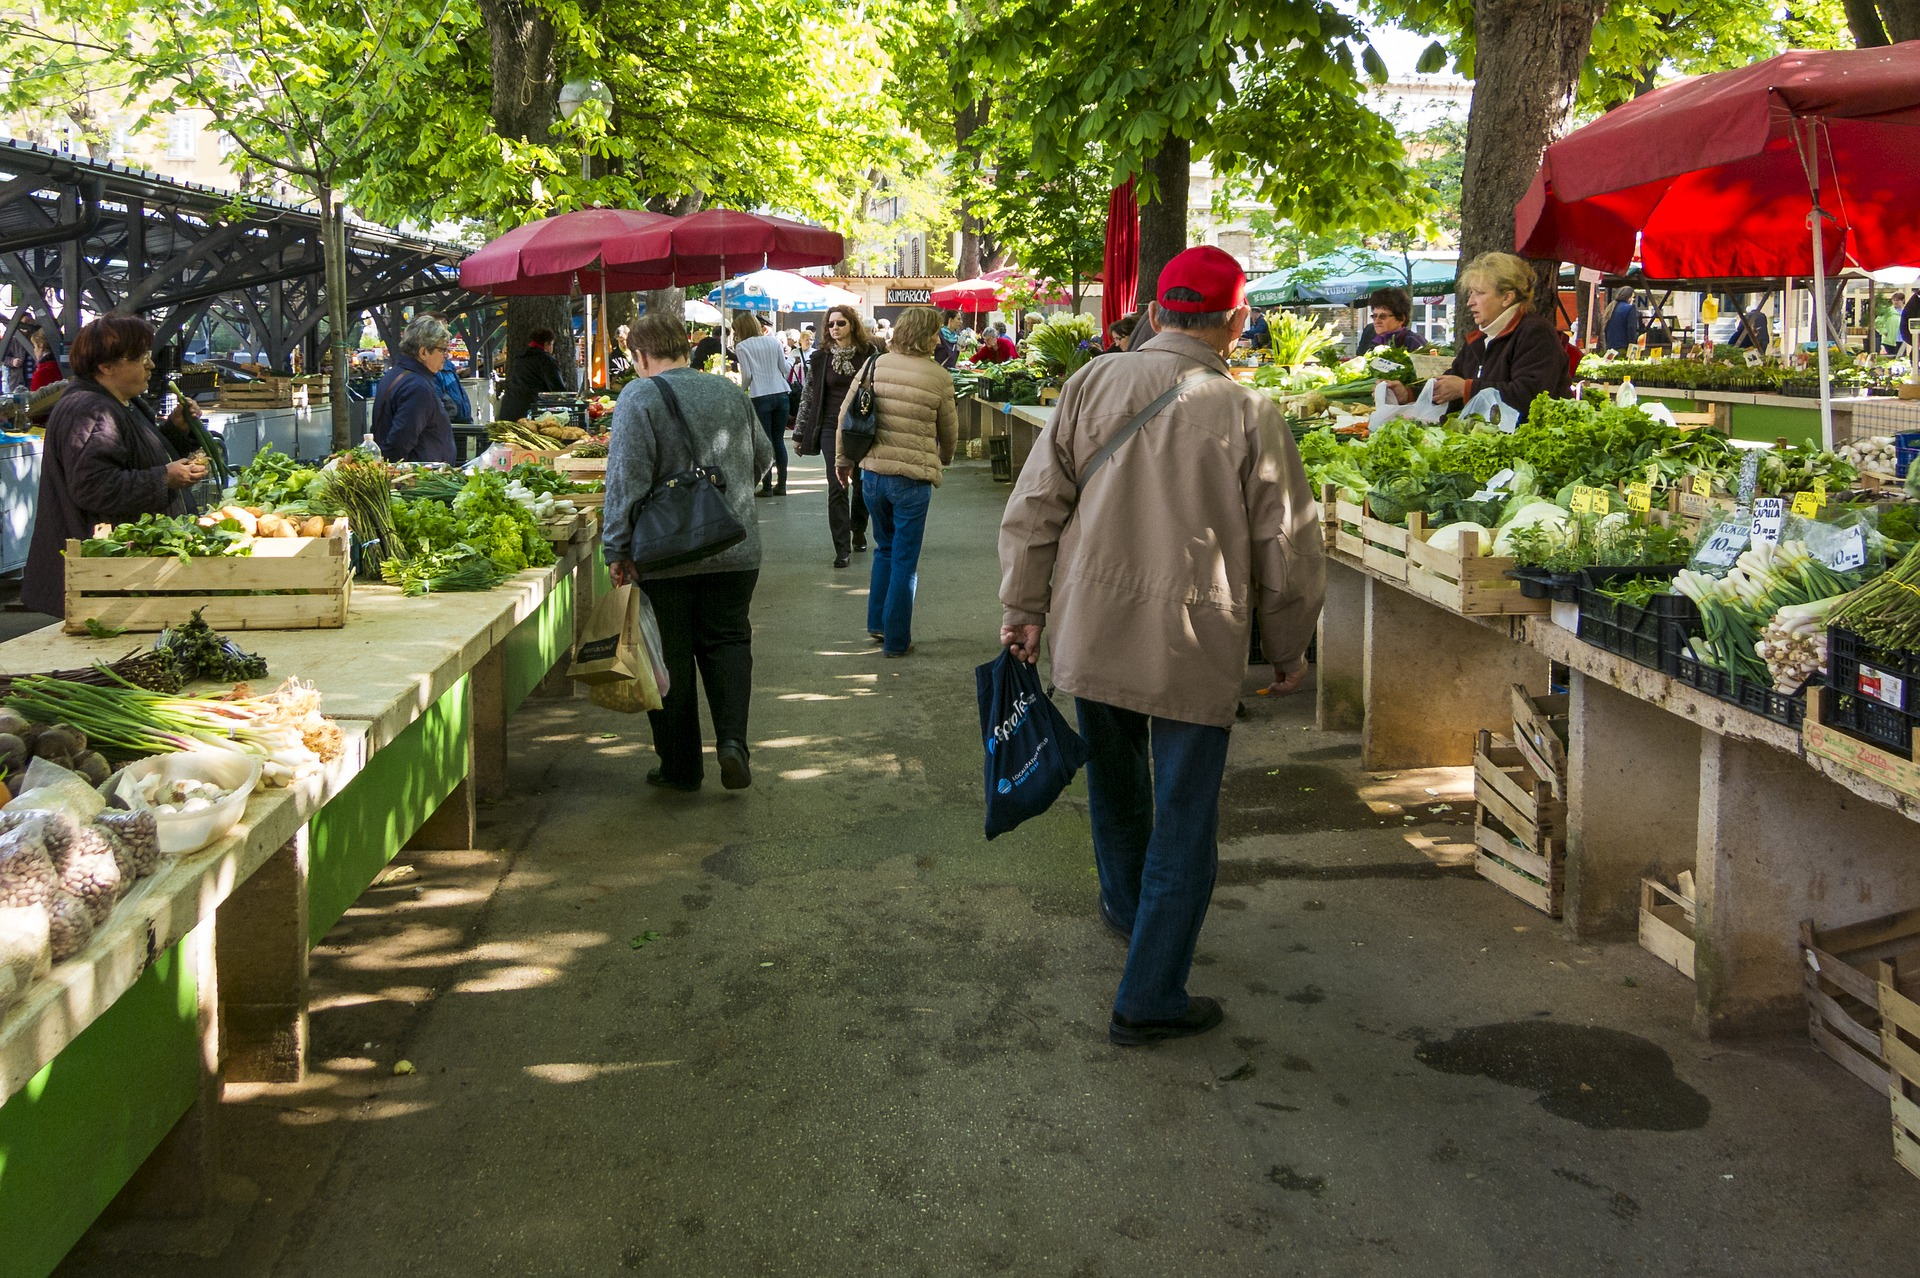
\includegraphics[width=\linewidth]{external/jpg-source/3.4.B6 Act 1 Launch.jpg}
\end{image}%
Un agricultor tiene 14 cebollas y 2 bolsas. Pone el mismo número de cebollas en cada bolsa.%
\par
Lin dice que la situación debe representarse con la ecuación:%
\begin{equation*}
2 \times \boxed{\phantom{3}} = 14
\end{equation*}
%
\par
Mai dice que la situación debe representarse con la ecuación:%
\begin{equation*}
14 \div 2 = \boxed{\phantom{3}}
\end{equation*}
%
\par
¿Con qué ecuación estás de acuerdo? Prepárate para explicar tu razonamiento.%
\par\smallskip%
\noindent\textbf{\blocktitlefont Solución}.\hypertarget{act-ecuacionesCebollas-3}{}\quad{}Ejemplos de respuestas:%
%
\begin{itemize}[label=\textbullet]
\item{}Lin, porque sabemos el total y cuántos grupos hay, pero no sabemos cuántos hay en cada grupo, así que uno de los factores es desconocido.%
\item{}Mai, porque sabemos que el total se está dividiendo en 2 grupos, así que estamos dividiendo para encontrar el número en cada grupo.%
\end{itemize}
\end{activity}%
\footnotetext[37]{\nolinkurl{pixabay.com/photos/market-vegetable-market-1558658/}\label{act-ecuacionesCebollas-2-1-2-1-2}}%
\par
\begin{paragraphs}{Síntesis de la actividad.}{act-ecuacionesCebollas-5-1}%
%
\begin{itemize}[label=\textbullet]
\item{}``Después de discutir sus ideas con su compañero, ¿con quién están de acuerdo? Expliquen su razonamiento''%
\item{}Si los estudiantes no identifican que tanto Lin como Mai tienen razón, considere preguntar, ``¿De qué manera pueden ambas ecuaciones representar esta situación?''%
\end{itemize}
\end{paragraphs}%
\begin{paragraphs}{Desarrollo de lenguaje matemático.}{act-ecuacionesCebollas-5-2}%
MLR7 Comparar y Conectar. Síntesis: Crea una presentación visual del problema. ``¿Qué tenían en común las estrategias de Lin y Mai? ¿En qué son diferentes?'' A medida que los estudiantes comparten su razonamiento, muestra las conexiones en la presentación. Por ejemplo, debajo de cada ecuación, escribe las palabras ``total'', ``número de grupos'' y ``número en cada grupo'' dependiendo de la ecuación y la contribución de los estudiantes. Avances: Escuchar, Representar%
\end{paragraphs}%
\end{subsubsectionptx}
%
%
\typeout{************************************************}
\typeout{Subsubsección  Actividad 2~(20 mins)}
\typeout{************************************************}
%
\begin{subsubsectionptx}{Subsubsección}{Actividad 2~(20 mins)}{}{Actividad 2}{}{}{lec-divisionComoFactorDesconocido-act2}
\par
\begin{paragraphs}{Tiempo recomendado.}{act-enElMercadoAgricola-4-1}%
20 minutos%
\end{paragraphs}%
\begin{paragraphs}{Narrativa.}{act-enElMercadoAgricola-4-2}%
El propósito de esta actividad es que los estudiantes comprendan cómo las ecuaciones de multiplicación corresponden a diagramas y ecuaciones que han utilizado para representar situaciones de división. El enfoque debe estar en relacionar el factor desconocido con el número desconocido de grupos o el número desconocido de objetos en cada grupo. En sus explicaciones, los estudiantes deben hacer conexiones directas entre las situaciones, representaciones y ecuaciones (MP2).%
\end{paragraphs}%
\begin{paragraphs}{Materiales.}{act-enElMercadoAgricola-4-3}%
%
\begin{itemize}[label=\textbullet]
\item{}Tabla para rellenar. Una tabla para cada pareja (disponible en el libro de trabajo o \href{external/act-pdf/act-enElMercadoAgricola.pdf}{descargar para imprimir}\footnotemark{}).%
\end{itemize}
\end{paragraphs}%
\begin{paragraphs}{Lanzamiento.}{act-enElMercadoAgricola-4-4}%
%
\begin{itemize}[label=\textbullet]
\item{}Grupos de 2%
\item{}``Vamos a completar esta tabla. Tómense un minuto para ver qué está faltando en la tabla''%
\item{}1 minuto: tiempo para pensar en silencio%
\item{}Aclare cualquier pregunta que tengan los estudiantes sobre las situaciones que aparecen en la tabla.%
\end{itemize}
\end{paragraphs}%
\begin{paragraphs}{Desarrollo de la actividad.}{act-enElMercadoAgricola-4-5}%
%
\begin{itemize}[label=\textbullet]
\item{}``Completen cada fila. Prepárense para explicar su razonamiento''%
\item{}5-7 minutos: tiempo de trabajo individual%
\item{}``Compartan con su compañero cómo razonaron''%
\item{}2-3 minutos: discusión en pareja%
\item{}Escuche las distintas maneras en las que los estudiantes explican sus respuestas. Identifique estrategias que establezcan conexiones claras entre las cantidades que aparecen en cada situación y sus representaciones.%
\item{}Si los estudiantes terminan antes de lo planeado, o si considera apropiado agregar movimiento a la actividad, considere hacer grupos de 4 y pedirles que creen un póster que muestre su propia situación, el dibujo correspondiente, la ecuación de multiplicación y la ecuación de división. Luego pueden hacer un recorrido por el salón.%
\end{itemize}
\end{paragraphs}%
\begin{activity}{Actividad}{En el mercado agrícola.}{act-enElMercadoAgricola}%
Completa cada fila. Prepárate para explicar tu razonamiento.%
\begin{image}{0}{1}{0}{}%
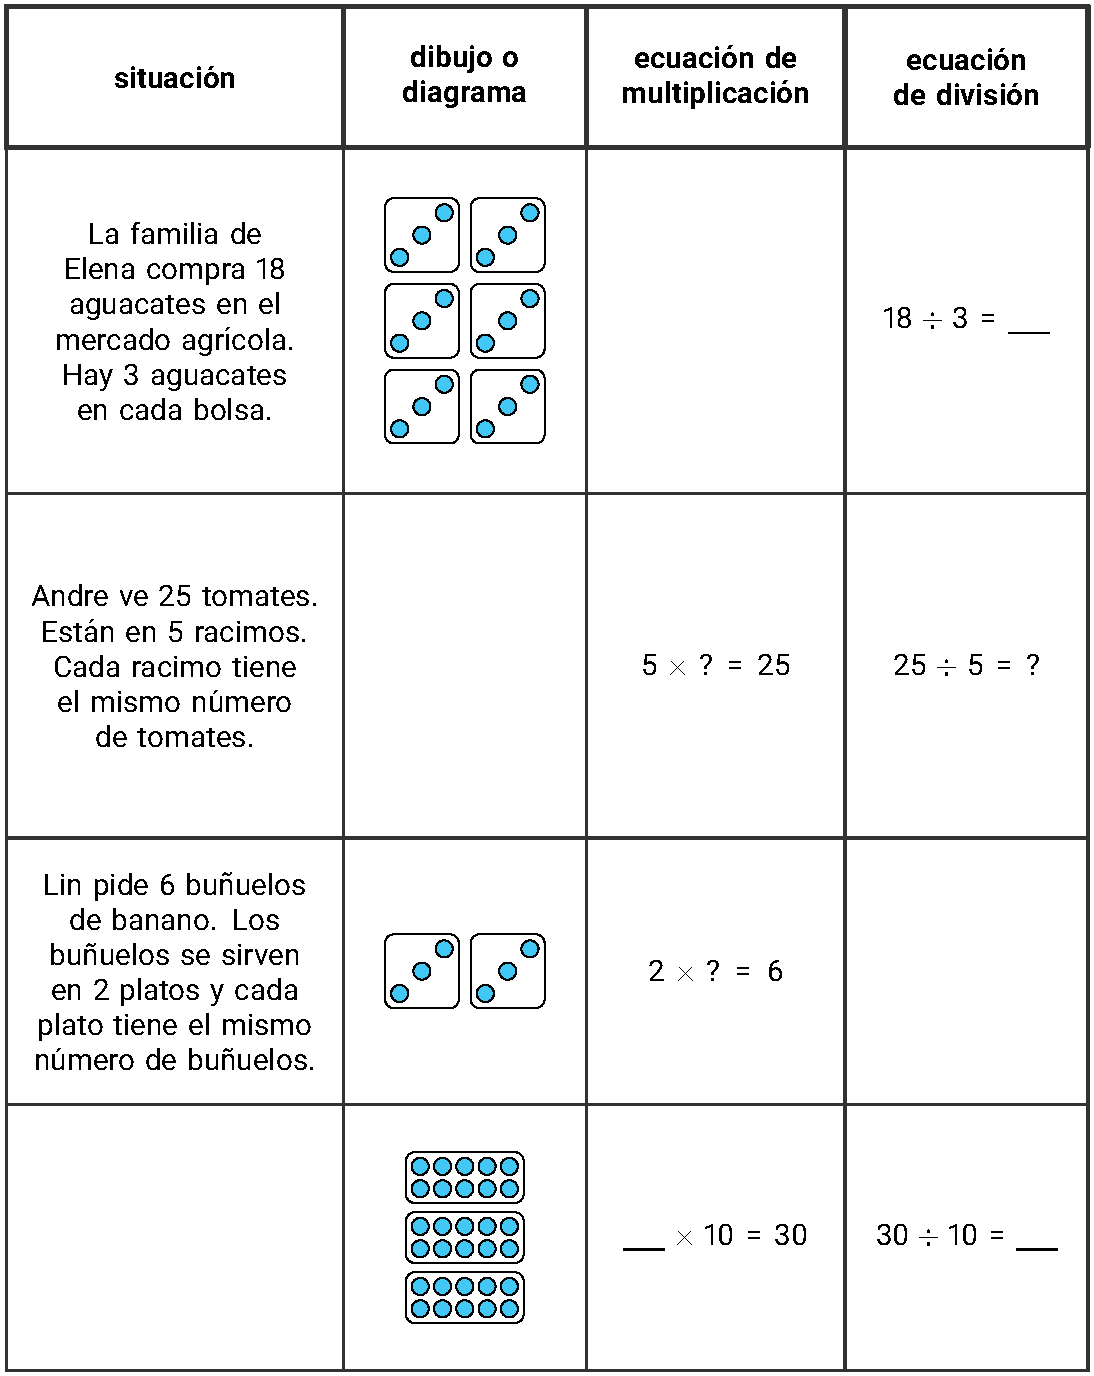
\includegraphics[width=\linewidth]{external/tikz-source/enElMercadoAgricola-tab.pdf}
\end{image}%
\par\smallskip%
\noindent\textbf{\blocktitlefont Solución}.\hypertarget{act-enElMercadoAgricola-3}{}\quad{}\begin{image}{0}{1}{0}{}%
\includegraphics[width=\linewidth]{external/tikz-source/enElMercadoAgricola-tab-sol.pdf}
\end{image}%
\end{activity}%
\footnotetext[38]{\nolinkurl{external/act-pdf/act-enElMercadoAgricola.pdf}\label{act-enElMercadoAgricola-4-3-2-1-2}}%
\par
\begin{paragraphs}{Para los estudiantes con dificultades.}{act-enElMercadoAgricola-5-1}%
Si en una cierta fila los estudiantes no registran la ecuación de multiplicación o la ecuación de división, considere preguntar:%
%
\begin{itemize}[label=\textbullet]
\item{}``¿Cómo decidirías qué tipo de ecuación escribir?''%
\item{}``¿Cómo podríamos representar este diagrama (o situación) con una ecuación de multiplicación (o división)? ¿En dónde vemos cada parte de la ecuación en el diagrama (o situación)?''%
\end{itemize}
\end{paragraphs}%
\begin{paragraphs}{Síntesis de la actividad.}{act-enElMercadoAgricola-5-2}%
%
\begin{itemize}[label=\textbullet]
\item{}Comparta las respuestas de los estudiantes para cada fila.%
\item{}Considere preguntar ``¿Cómo muestra la ecuación (o el dibujo) los números o las cantidades de la situación?''%
\item{}``¿Qué relación vieron entre las ecuaciones de multiplicación y las ecuaciones de división?'' (Las ecuaciones usan los mismos números para representar la situación. La respuesta de la ecuación de división siempre es uno de los factores desconocidos de la ecuación de multiplicación.)%
\end{itemize}
\end{paragraphs}%
\begin{paragraphs}{Acceso a estudiantes con discapacidades.}{act-enElMercadoAgricola-5-3}%
Involucramiento: Desarrollar el esfuerzo y la persistencia. Algunos estudiantes pueden beneficiarse de retroalimentación que enfatice el esfuerzo y el tiempo dedicado a la tarea. Por ejemplo, dar retroalimentación después de cada fila o motivar a los estudiantes a trabajar en la siguiente fila si tienen dificultades con una fila específica.%
\par
Apoya la accesibilidad para: Atención, Funcionamiento Social-Emocional.%
\end{paragraphs}%
\end{subsubsectionptx}
%
%
\typeout{************************************************}
\typeout{Subsubsección  Síntesis de la lección~(10 mins)}
\typeout{************************************************}
%
\begin{subsubsectionptx}{Subsubsección}{Síntesis de la lección~(10 mins)}{}{Síntesis de la lección}{}{}{lec-divisionComoFactorDesconocido-sintesis}
``Hoy nos concentramos en conectar ecuaciones de multiplicación y ecuaciones de división que representan la misma situación.''%
\par
Por ejemplo:%
\begin{assemblage}{Conjunto}{}{lec-divisionComoFactorDesconocido-sintesis-6}%
Un agricultor pone 14 cebollas en 2 bolsas con la misma cantidad de cebollas en cada bolsa.%
\begin{equation*}
\displaystyle 2 \times \boxed{\phantom{3}} = 14
\end{equation*}
%
\begin{equation*}
14 \div 2 = \boxed{\phantom{3}}
\end{equation*}
%
\end{assemblage}
``Estas dos ecuaciones tienen las mismas partes: 2, 14 y una cantidad desconocida. ¿Por qué están organizadas de una manera diferente si representan la misma situación?'' (En multiplicación, los factores son la cantidad de grupos y el tamaño de cada grupo. El número del otro lado de la ecuación es el total. En división, comenzamos con el total y dividimos por la cantidad de grupos que tenemos para encontrar el tamaño del grupo, o dividimos por el tamaño del grupo para encontrar la cantidad de grupos que tenemos, esa es la respuesta.)%
\par
Llamamos \terminology{cociente} al resultado de una ecuación de división. Por ejemplo, en \(14 \div 2 = \boxed{\phantom{3}}\), no conocemos el resultado, por lo que vamos a encontrar el valor del cociente. En la ecuación completa \(14 \div 2 = 7\), vemos que el valor del cociente es 7.%
\end{subsubsectionptx}
%
%
\typeout{************************************************}
\typeout{Preguntas de comprensión  Actividad de cierre~(5 mins)}
\typeout{************************************************}
%
\begin{reading-questions-subsubsection}{Preguntas de comprensión}{Actividad de cierre~(5 mins)}{}{Actividad de cierre}{}{}{lec-divisionComoFactorDesconocido-cool}
\href{external/cools-pdf/cool-muffinsEnCajas-standalone.pdf}{Descargar pdf para imprimir o proyectar}\footnote{\nolinkurl{external/cools-pdf/cool-muffinsEnCajas-standalone.pdf}\label{lec-divisionComoFactorDesconocido-cool-5}}\begin{project}{Actividad de cierre}{Muffins en cajas.}{cool-muffinsEnCajas}%
Hay 30 \emph{muffins} y varias cajas para la feria de pastelería. En cada caja hay 6 \emph{muffins}. ¿Cuántas cajas hay?%
\begin{sidebyside}{2}{0.05}{0.05}{0.1}%
\begin{sbspanel}{0.4}%
Tyler escribió dos ecuaciones para este problema.%
\end{sbspanel}%
\begin{sbspanel}{0.4}%
\(\underline{\hspace{1 cm}} \times 6 = 30\)%
\par
\(30 \div 6 = \underline{\hspace{1 cm}}\)%
\end{sbspanel}%
\end{sidebyside}%
\par
Él dice que en cada espacio en blanco va el mismo número, aunque una ecuación es de multiplicación y la otra es de división. ¿Tiene razón? Explica o muestra tu razonamiento.%
\par\smallskip%
\noindent\textbf{\blocktitlefont Solución}.\hypertarget{cool-muffinsEnCajas-3}{}\quad{}Tyler tiene razón. Ejemplo de respuesta: El cinco va en ambos espacios en blanco. Lo escribimos en diferentes lugares para ecuaciones de multiplicación y división.%
\end{project}%
\par
\begin{paragraphs}{Posibles errores.}{cool-muffinsEnCajas-4-1}%
Los estudiantes dicen que se deben usar números diferentes para completar cada ecuación.%
\end{paragraphs}%
\begin{paragraphs}{Acciones para apoyar el aprendizaje.}{cool-muffinsEnCajas-4-2}%
Durante el lanzamiento de la actividad del día siguiente, reparta la actividad de cierre y haga que los estudiantes discutan cómo el número faltante en ambas ecuaciones se relaciona con la situación.%
\end{paragraphs}%
\end{reading-questions-subsubsection}
\end{subsectionptx}
%
%
\typeout{************************************************}
\typeout{Subsección  Lección 7 -~Relacionemos multiplicación y división}
\typeout{************************************************}
%
\begin{subsectionptx}{Subsección}{Lección 7 -~Relacionemos multiplicación y división}{}{Lección 7}{}{}{lec-relacionarMultiplicacionYDivision}
\begin{objectives}{Objetivos de aprendizaje}{lec-relacionarMultiplicacionYDivision-4}
%
\begin{itemize}[label=\textbullet]
\item{}Representar situaciones que involucran grupos iguales usando ecuaciones de multiplicación y división con un símbolo para la cantidad desconocida.%
\item{}Usar la multiplicación y la división con números hasta 100 para resolver problemas que involucren grupos iguales.%
\end{itemize}
\end{objectives}
\begin{introduction}{}%
\begin{paragraphs}{Estándares CCSS asociados.}{lec-relacionarMultiplicacionYDivision-5-1}%
3.NBT.A.3, 3.OA.A.2, 3.OA.A.3, 3.OA.B.6%
\end{paragraphs}%
\begin{paragraphs}{Momentos de la lección.}{lec-relacionarMultiplicacionYDivision-5-2}%
\noindent
\begin{longtable}[l]{ll}
\addtocounter{table}{-1}
\endfirsthead
\endhead
\multicolumn{2}{r}{(Continúa en la página siguiente)}\\
\endfoot
\endlastfoot
\hyperref[lec-relacionarMultiplicacionYDivision-warm]{Subsubsección }& Calentamiento~(10 mins)\\
\hyperref[lec-relacionarMultiplicacionYDivision-act1]{Subsubsección }& Actividad 1~(20 mins)\\
\hyperref[lec-relacionarMultiplicacionYDivision-act2]{Subsubsección }& Actividad 2~(15 mins)\\
\hyperref[lec-relacionarMultiplicacionYDivision-sintesis]{Subsubsección }& Síntesis de la lección~(10 mins)\\
\hyperref[lec-relacionarMultiplicacionYDivision-cool]{Preguntas de comprensión }& Actividad de cierre~(5 mins)\\
\end{longtable}
\end{paragraphs}%
\begin{paragraphs}{Propósito de la lección.}{lec-relacionarMultiplicacionYDivision-5-3}%
El propósito de esta lección es que los estudiantes utilicen la relación entre la multiplicación y la división para escribir ecuaciones y resolver problemas.%
\end{paragraphs}%
\begin{paragraphs}{Materiales.}{lec-relacionarMultiplicacionYDivision-5-4}%
%
\begin{itemize}[label=\textbullet]
\item{}Actividad 1%
%
\begin{itemize}[label=$\circ$]
\item{}Una hoja de registro para cada estudiante (en el libro de trabajo, o \href{external/blm/pdf-source/mesa-redonda-de-division.pdf}{descargar para imprimir}\footnote{\nolinkurl{external/blm/pdf-source/mesa-redonda-de-division.pdf}\label{lec-relacionarMultiplicacionYDivision-5-4-2-1-2-1-2}})%
\end{itemize}
\end{itemize}
\end{paragraphs}%
\begin{paragraphs}{Narrativa de la lección.}{lec-relacionarMultiplicacionYDivision-5-5}%
En lecciones anteriores, los estudiantes aprendieron sobre la división y cómo se relaciona con la multiplicación. En esta lección, usan diferentes formas de representación para mostrar esta relación y escriben ecuaciones para situaciones de división.%
\end{paragraphs}%
\begin{paragraphs}{Preguntas de reflexión.}{lec-relacionarMultiplicacionYDivision-5-6}%
¿Qué pregunta de las que hizo ayudó más a los estudiantes a entender la relación entre las ecuaciones de multiplicación y las de división? ¿Cómo demostraron los estudiantes que la pregunta fue efectiva?%
\end{paragraphs}%
\end{introduction}%
%
%
\typeout{************************************************}
\typeout{Subsubsección  Calentamiento~(10 mins)}
\typeout{************************************************}
%
\begin{subsubsectionptx}{Subsubsección}{Calentamiento~(10 mins)}{}{Calentamiento}{}{}{lec-relacionarMultiplicacionYDivision-warm}
\par
\begin{paragraphs}{Tiempo recomendado.}{warm-cuantosVes-decenas-4-1}%
10 minutos%
\end{paragraphs}%
\begin{paragraphs}{Narrativa.}{warm-cuantosVes-decenas-4-2}%
El propósito de esta actividad tipo ``Cuántos Ves'' es que los estudiantes utilicen estrategias de agrupación para describir las imágenes que ven.%
\par
Cuando los estudiantes utilizan la agrupación para encontrar el total en un múltiplo de diez, buscan y hacen uso de estructuras.%
\end{paragraphs}%
\begin{paragraphs}{Lanzamiento.}{warm-cuantosVes-decenas-4-3}%
%
\begin{itemize}[label=\textbullet]
\item{}Grupos de 2%
\item{}``¿Cuántos ven? ¿Cómo lo saben?, ¿qué ven?''%
\item{}Muestre rápidamente la imagen.%
\item{}30 segundos: tiempo para pensar en silencio%
\end{itemize}
\end{paragraphs}%
\begin{paragraphs}{Desarrollo de la actividad.}{warm-cuantosVes-decenas-4-4}%
%
\begin{itemize}[label=\textbullet]
\item{}Muestre la imagen.%
\item{}``Discutan con su compañero cómo pensaron''%
\item{}1 minuto: discusión con el compañero%
\item{}Registre las respuestas.%
\end{itemize}
\end{paragraphs}%
\begin{exploration}{Calentamiento}{Cuántos ves: Decenas.}{warm-cuantosVes-decenas}%
¿Cuántos ves?\\
 ¿Cómo lo sabes?, ¿qué ves?%
\begin{image}{0}{1}{0}{}%
\includegraphics[width=\linewidth]{external/svg-source/tikz-file-147480-scale13.pdf}
\end{image}%
\par\smallskip%
\noindent\textbf{\blocktitlefont Solución}.\hypertarget{warm-cuantosVes-decenas-3}{}\quad{}60. Ejemplos de respuesta:%
%
\begin{itemize}[label=\textbullet]
\item{}Veo 6 grupos de 10.%
\item{}Veo 2 decenas en cada fila y hay 3 filas, así que hay 6 decenas.%
\item{}Veo 2 decenas en cada grupo y hay 3 grupos, así que hay 6 decenas.%
\item{}Veo 2 grupos con 3 decenas en cada grupo, así que hay 6 decenas.%
\end{itemize}
\end{exploration}%
\par
\begin{paragraphs}{Síntesis de la actividad.}{warm-cuantosVes-decenas-5-1}%
%
\begin{itemize}[label=\textbullet]
\item{}``¿Qué expresiones podríamos escribir para representar las diferentes formas en las que los estudiantes vieron las decenas?'' (\(6\times 10\), porque algunos estudiantes vieron 6 filas de 10. \(3 \times (10 \times 2)\), porque algunos estudiantes vieron 2 filas de 10 y luego multiplicaron por 3. \((3 \times 10) \times 2\), porque algunos estudiantes vieron 3 decenas en la columna de la izquierda y luego multiplicaron por 2.)%
\item{}Considere preguntar:%
%
\begin{itemize}[label=$\circ$]
\item{}``¿Alguien puede expresar con otras palabras la forma en la que \fillintext{10} vio las decenas?''%
\item{}``¿Alguien vio las decenas de la misma forma, pero lo explicaría de otra manera?''%
\item{}``¿Alguien quiere compartir otra observación sobre la forma en la que \fillintext{10} vio las decenas?''%
\end{itemize}
\end{itemize}
\end{paragraphs}%
\end{subsubsectionptx}
%
%
\typeout{************************************************}
\typeout{Subsubsección  Actividad 1~(20 mins)}
\typeout{************************************************}
%
\begin{subsubsectionptx}{Subsubsección}{Actividad 1~(20 mins)}{}{Actividad 1}{}{}{lec-relacionarMultiplicacionYDivision-act1}
\par
\begin{paragraphs}{Tiempo recomendado.}{act-mesaRedondaDeDivision-4-1}%
20 minutos%
\end{paragraphs}%
\begin{paragraphs}{Narrativa.}{act-mesaRedondaDeDivision-4-2}%
El propósito de esta actividad es que los estudiantes consoliden lo que han aprendido sobre la relación entre la multiplicación y la división. Los estudiantes comienzan creando un dibujo de grupos iguales. Luego reciben un dibujo creado por otro estudiante de su grupo y escriben una situación de división que le corresponda. Después pasan su hoja a otro estudiante y reciben otra hoja y utilizan el dibujo de grupos iguales y la situación para escribir una ecuación de multiplicación. En la última ronda de esta estructura de “carrusel”, los estudiantes escriben una ecuación de división que corresponda con las otras representaciones.%
\par
Cuando los estudiantes relacionan dibujos, situaciones y ecuaciones, razonan de manera abstracta y cuantitativa (MP2). Al mirar el trabajo de los demás, los estudiantes pueden agregar observaciones a las representaciones y pueden defender diferentes puntos de vista. Los estudiantes pueden criticar el trabajo de otros y construir argumentos razonables (MP3).%
\par
Cada estudiante trabaja en una hoja, pero todos trabajan en la misma casilla del organizador gráfico. Por lo tanto, anímelos a hablar con su grupo si tienen dificultades. En cada ronda, recuérdeles a los estudiantes que lo que están creando debe coincidir con lo que sus compañeros completaron en esa misma hoja en rondas anteriores.%
\end{paragraphs}%
\begin{paragraphs}{Materiales.}{act-mesaRedondaDeDivision-4-3}%
%
\begin{itemize}[label=\textbullet]
\item{}Una hoja de registro para cada estudiante (en el libro de trabajo, o \href{external/blm/pdf-source/mesa-redonda-de-division.pdf}{descargar para imprimir}\footnotemark{})%
\end{itemize}
\end{paragraphs}%
\begin{paragraphs}{Lanzamiento.}{act-mesaRedondaDeDivision-4-4}%
%
\begin{itemize}[label=\textbullet]
\item{}Grupos de 4%
\item{}Entregue a cada estudiante una hoja de registro.%
\item{}``En el primer recuadro de su hoja, hagan un dibujo que muestre grupos iguales de objetos. Los demás estudiantes del grupo van a usar este dibujo para completar los otros recuadros''%
\item{}3 minutos: tiempo de trabajo individual%
\end{itemize}
\end{paragraphs}%
\begin{paragraphs}{Desarrollo de la actividad.}{act-mesaRedondaDeDivision-4-5}%
%
\begin{itemize}[label=\textbullet]
\item{}``Pásenle su hoja al compañero que está a su derecha. En el recuadro 2, escriban una descripción de una situación de división que corresponda al dibujo que les acabaron de pasar''.%
\item{}3 minutes: tiempo de trabajo individual%
\item{}``Pasen su hoja a la derecha. En el recuadro 3, escriban una ecuación de multiplicación que corresponda al dibujo y a la situación de división que acabaron de recibir. Usen un símbolo para representar la cantidad desconocida''.%
\item{}2 minutes: tiempo de trabajo individual%
\item{}``Pasen su hoja a la derecha. En el recuadro 4, escriban una ecuación de división que corresponda al dibujo, a la situación de división y a la ecuación de multiplicación que acabaron de recibir. Usen un símbolo para representar la cantidad desconocida''%
\item{}2 minutes: tiempo de trabajo individual%
\item{}``Pasen su hoja a la derecha una vez más. Cada uno debería recibir su dibujo original de vuelta''%
\item{}``Hablen con su grupo sobre cuál recuadro les pareció más difícil de completar. Compartan ideas acerca de qué fue lo que más les ayudó durante esta actividad''%
\item{}5 minutes: discusión en grupos pequeños%
\end{itemize}
\end{paragraphs}%
\begin{activity}{Actividad}{Mesa redonda de división.}{act-mesaRedondaDeDivision}%
Tu profesor te dará una hoja de papel con 4 recuadros. La actividad tiene 4 rondas. En cada ronda trabajarás en una hoja distinta y tu profesor te pedirá que dibujes o escribas algo en uno de los recuadros.%
\par
Después de trabajar en cada recuadro, haz una pausa y espera a que el profesor te dé las instrucciones de la siguiente ronda.%
%
\begin{enumerate}
\item{}En el recuadro 1 de tu hoja, haz un dibujo de grupos iguales.%
\item{}Observa el dibujo que tu compañero dibujó en la hoja que acabaste de recibir. En el recuadro 2, escribe una descripción de una situación de división que corresponda a ese dibujo.%
\item{}Observa los recuadros 1 y 2 de la hoja que acabaste de recibir. En el recuadro 3, escribe una ecuación de multiplicación que corresponda al dibujo y a la situación de división de esa hoja. Usa un símbolo para representar la cantidad desconocida.%
\item{}Observa los recuadros 1, 2 y 3 de la hoja que acabaste de recibir. En el recuadro 4, escribe una ecuación de división que corresponda al dibujo, a la situación de división y a la ecuación de multiplicación. Usa un símbolo para representar la cantidad desconocida.%
\end{enumerate}
\begin{image}{0.2}{0.6}{0.2}{}%
\includegraphics[width=\linewidth]{external/png-source/CS 3.4 Lesson 7 Activity 1.png}
\end{image}%
\par\smallskip%
\noindent\textbf{\blocktitlefont Solución}.\hypertarget{act-mesaRedondaDeDivision-3}{}\quad{}Las respuestas pueden variar. Ejemplo de solución:%
\par
Recuadro 1: 3 grupos con 4 objetos en cada grupo. Recuadro 2: Lin tiene 12 limones y quiere repartirlos en 3 grupos del mismo tamaño. ¿Cuántos limones puede poner en cada grupo? Recuadro 3: \(3 \times {?} = 12\). Recuadro 4: \(12 \div 3 = {?} \)%
\end{activity}%
\footnotetext[41]{\nolinkurl{external/blm/pdf-source/mesa-redonda-de-division.pdf}\label{act-mesaRedondaDeDivision-4-3-2-1-2}}%
\par
\begin{paragraphs}{Síntesis de la actividad.}{act-mesaRedondaDeDivision-5-1}%
%
\begin{itemize}[label=\textbullet]
\item{}``¿Qué estrategias compartieron en su grupo?'' (Cuando no estaba seguro de cómo escribir una situación, volví a mirar el dibujo e intenté imaginar algo que pudiera estar dividiendo que se pareciera al dibujo. Cuando estaba escribiendo una ecuación, me ayudó a imaginar que la situación estaba ocurriendo.)%
\item{}``Al examinar su hoja, ¿qué conexiones observan entre la multiplicación y la división?'' (Puedo usar tanto la multiplicación como la división para representar el mismo dibujo o situación. En todas las ecuaciones de multiplicación hay un factor desconocido, pero en las ecuaciones de división todas lo que es desconocido es el cociente.)%
\end{itemize}
\end{paragraphs}%
\begin{paragraphs}{Acceso a estudiantes con discapacidades.}{act-mesaRedondaDeDivision-5-2}%
Participación: Desarrollar el esfuerzo y la persistencia. Dé a cada grupo retroalimentación que fomente la colaboración y la creación de comunidad. Por ejemplo, apoye a los estudiantes para que participen, para que pasen la hoja a la derecha y escriban el símbolo.%
\par
Apoya la accesibilidad para: Funcionamiento social-emocional, Lenguaje%
\end{paragraphs}%
\end{subsubsectionptx}
%
%
\typeout{************************************************}
\typeout{Subsubsección  Actividad 2~(15 mins)}
\typeout{************************************************}
%
\begin{subsubsectionptx}{Subsubsección}{Actividad 2~(15 mins)}{}{Actividad 2}{}{}{lec-relacionarMultiplicacionYDivision-act2}
\par
\begin{paragraphs}{Tiempo recomendado.}{act-gruposUtilesEscolares-4-1}%
15 minutos%
\end{paragraphs}%
\begin{paragraphs}{Narrativa.}{act-gruposUtilesEscolares-4-2}%
En esta actividad, los estudiantes resolverán problemas de grupos iguales. Pueden elegir resolver el problema o escribir la ecuación primero, dependiendo del orden que les parezca más lógico. Deben usar un símbolo para la cantidad desconocida y pueden escribir una ecuación de multiplicación o división. Al final, se destacarán una ecuación de multiplicación y una de división que representen el mismo problema.%
\end{paragraphs}%
\begin{paragraphs}{Lanzamiento.}{act-gruposUtilesEscolares-4-3}%
%
\begin{itemize}[label=\textbullet]
\item{}Grupos de 2%
\item{}``Todas estas situaciones son acerca de cosas que pueden encontrar en un pupitre o alrededor del pupitre. ¿Qué cosas podrían encontrar en un pupitre o a su alrededor?''%
\item{}30 segundos: tiempo para pensar en silencio%
\item{}Compartir respuestas.%
\end{itemize}
\end{paragraphs}%
\begin{paragraphs}{Desarrollo de la actividad.}{act-gruposUtilesEscolares-4-4}%
%
\begin{itemize}[label=\textbullet]
\item{}``Lean cada situación y escriban una ecuación para cada una. Usen un símbolo para representar la cantidad desconocida. Después, resuelvan la ecuación y encuentren el número desconocido. Pueden resolver el problema primero o escribir una ecuación primero dependiendo de qué tenga más sentido para ustedes. Prepárense para explicar su razonamiento.''%
\item{}7–10 minutos: tiempo de trabajo individual%
\item{}Identifique a los estudiantes que escriben una ecuación de división y una ecuación de multiplicación para la misma situación para que las compartan durante la síntesis.%
\item{}``Ahora, por turnos, compartan sus ecuaciones y soluciones con su compañero.''%
\item{}3–5 minutos: discusión en pareja%
\end{itemize}
\end{paragraphs}%
\begin{activity}{Actividad}{Grupos de útiles escolares.}{act-gruposUtilesEscolares}%
En cada situación:%
\par
(a) Escribe una ecuación que represente la situación. Usa un símbolo para representar la cantidad desconocida.%
\par
(b) Resuelve el problema y encuentra el número desconocido de la ecuación. Prepárate para explicar tu razonamiento.%
\par
Situaciones:%
%
\begin{enumerate}
\item{}Kiran tenía 32 clips y los repartió entre varios estudiantes. Le dio 4 clips a cada uno. ¿Cuántos estudiantes recibieron clips?%
\item{}Hay 28 libros distribuidos en 4 pilas. Si cada pila tiene la misma cantidad de libros, ¿cuántos libros hay en cada pila?%
\item{}Hay 6 cajas. En cada caja hay 8 borradores. ¿Cuántos borradores hay en total?%
\item{}Lin tenía 36 notas adhesivas y varios cuadernos. Ella puso 6 notas adhesivas en cada cuaderno. ¿En cuántos cuadernos puso notas adhesivas?%
\end{enumerate}
\par\smallskip%
\noindent\textbf{\blocktitlefont Solución}.\hypertarget{act-gruposUtilesEscolares-3}{}\quad{}%
\begin{enumerate}
\item{}%
\begin{enumerate}
\item{}\(4 \times {?} = 32\), \({?} \times 4 = 32\), o \(32 \div 4 = {?} \)%
\item{}8 estudiantes. Ejemplo de razonamiento:%
\begin{image}{0}{1}{0}{}%
\includegraphics[width=\linewidth]{external/svg-source/tikz-file-149318.pdf}
\end{image}%
Dibujé grupos de 4 hasta llegar a 32, luego conté los grupos. Había 8 grupos, entonces 8 estudiantes recibieron clips de papel.%
\end{enumerate}
%
\item{}%
\begin{enumerate}
\item{}\(4 \times \underline{\hspace{1 cm}} = 28\), \(\underline{\hspace{1 cm}} \times 4 = 28\), o \(28 \div 4 = \underline{\hspace{1 cm}}\)%
\item{}7 libros. Ejemplo de razonamiento:%
\begin{image}{0}{1}{0}{}%
\includegraphics[width=\linewidth]{external/svg-source/tikz-file-149319.pdf}
\end{image}%
Comencé con 4 filas ya que los libros estaban en 4 pilas. Sabía que \(4 \times 7\) es 28, entonces puse 7 en cada fila.%
\end{enumerate}
%
\item{}%
\begin{enumerate}
\item{}\(6 \times 8 = {?}\), \(8 \times 6 = {?}\), \({?} \div 8 = 6\), \({?} \div 6 = 8\)%
\item{}48 borradores. Ejemplo de razonamiento:%
\begin{image}{0}{1}{0}{}%
\includegraphics[width=\linewidth]{external/svg-source/tikz-file-149320.pdf}
\end{image}%
Dibujé 6 rectángulos para mostrar las cajas y puse 8 puntos en cada círculo. Luego, conté el número total de puntos y obtuve 48. Otra opción: Sabía que \(5 \times 8\) es 40 y un grupo más de 8 es 48.%
\end{enumerate}
%
\item{}%
\begin{enumerate}
\item{}\(\underline{\hspace{1 cm}} \times 6 = 36\), \(6 \times \underline{\hspace{1 cm}} = 36\), o \(36 \div 6 = \underline{\hspace{1 cm}}\)%
\item{}6 cuadernos. Ejemplo de razonamiento:%
\begin{image}{0}{1}{0}{}%
\includegraphics[width=\linewidth]{external/svg-source/tikz-file-149321.pdf}
\end{image}%
Dibujé grupos de 6 hasta llegar a 36. Pude hacer 6 grupos, así que 6 cuadernos reciben notas adhesivas.%
\end{enumerate}
%
\end{enumerate}
\end{activity}%
\par
\begin{paragraphs}{Para los estudiantes con dificultades.}{act-gruposUtilesEscolares-5-1}%
Si los estudiantes no encuentran una solución a los problemas, considere preguntar: ``¿De qué se trata este problema?'' y ``¿Cómo puedes representar el problema?''%
\end{paragraphs}%
\begin{paragraphs}{Síntesis de la actividad.}{act-gruposUtilesEscolares-5-2}%
%
\begin{itemize}[label=\textbullet]
\item{}Invite a los estudiantes que escribieron una ecuación de división y una de multiplicación para la misma situación. Muestre las ecuaciones para que todos las vean.%
\item{}Discuta las diferencias en las ecuaciones que los estudiantes escribieron.%
\item{}Considere preguntar:%
\begin{itemize}[label=$\circ$]
\item{}``¿Cómo representa la situación cada número de las ecuaciones?''%
\item{}``\fillintext{10} escribió \fillintext{10} y \fillintext{10} escribió \fillintext{10} para representar el mismo problema. ¿En qué se parecen y en qué se diferencian esas ecuaciones?'' (Una de las ecuaciones es una ecuación de división y la otra es una ecuación de multiplicación con un factor desconocido. Usaron diferentes símbolos para la cantidad desconocida. Ambos símbolos en la ecuación representan la \fillintext{10} desconocida en la situación.)%
\end{itemize}
%
\item{}Invite a los estudiantes a compartir las estrategias que utilizaron para resolver el problema.%
\end{itemize}
\end{paragraphs}%
\begin{paragraphs}{Desarrollo de lenguaje matemático.}{act-gruposUtilesEscolares-5-3}%
MLR8 Soportes para la discusión: Antes de escribir las ecuaciones, invite a los estudiantes a entender el sentido de cada situación y a compartir con su compañero, por turnos, lo que entienden. Escuche y aclare cualquier pregunta sobre el contexto.%
\par
Avances: Lectura, Representación%
\end{paragraphs}%
\end{subsubsectionptx}
%
%
\typeout{************************************************}
\typeout{Subsubsección  Síntesis de la lección~(10 mins)}
\typeout{************************************************}
%
\begin{subsubsectionptx}{Subsubsección}{Síntesis de la lección~(10 mins)}{}{Síntesis de la lección}{}{}{lec-relacionarMultiplicacionYDivision-sintesis}
Muestre la ecuación: \(24 \div 4 = {?}\)%
\par
``¿Cuál sería la ecuación de multiplicación relacionada?'' (\(4 \times {?} = 24\) o \({?} \times 4 = 24\))%
\par
``¿Cómo se relacionan?'' (El número desconocido en la ecuación de división, es decir el cociente, es el número de grupos o el número en cada grupo y eso es lo que representa el número desconocido en la ecuación de multiplicación.)%
\par
Muestre: \(4 \times {?} = 28\) o \({?} \times 4 = 28\)%
\par
``¿Cuál sería la ecuación de división relacionada? (\(28 \div 4 = {?}\))''%
\par
``¿Cómo se relacionan?'' (En la ecuación de multiplicación se desconoce el número en cada grupo y eso es lo que representa el cociente en la ecuación de división.)%
\end{subsubsectionptx}
%
%
\typeout{************************************************}
\typeout{Preguntas de comprensión  Actividad de cierre~(5 mins)}
\typeout{************************************************}
%
\begin{reading-questions-subsubsection}{Preguntas de comprensión}{Actividad de cierre~(5 mins)}{}{Actividad de cierre}{}{}{lec-relacionarMultiplicacionYDivision-cool}
\href{external/cools-pdf/cool-rosasParaCompartir-standalone.pdf}{Descargar pdf para imprimir o proyectar}\footnote{\nolinkurl{external/cools-pdf/cool-rosasParaCompartir-standalone.pdf}\label{lec-relacionarMultiplicacionYDivision-cool-5}}\begin{project}{Actividad de cierre}{Rosas para compartir.}{cool-rosasParaCompartir}%
Clare tiene 14 rosas. Quiere darle 2 rosas a cada una de sus profesoras. ¿A cuántas profesoras les puede dar rosas?%
\par
Escribe una ecuación de multiplicación y una ecuación de división que representen la situación. Usa símbolos para representar los números desconocidos y explica tu razonamiento.%
\par\smallskip%
\noindent\textbf{\blocktitlefont Solución}.\hypertarget{cool-rosasParaCompartir-3}{}\quad{}\(?\times 2 = 14\) y \(14\div 2=?\)%
\par
Ejemplo de respuesta: Sé que ella tiene 14 rosas y quiere ponerlas en grupos de 2. La pregunta es sobre cuántos grupos habrá, que es cuántos profesores recibirán rosas y está representado por el "?".%
\par
Nota: Es muy importante que los estudiantes expliquen con precisión que conocen el tamaño de los grupos, pero no el número de grupos. Pueden invertir los factores en la ecuación de multiplicación.%
\end{project}%
\par
\begin{paragraphs}{Posibles errores.}{cool-rosasParaCompartir-4-1}%
Los estudiantes escriben una ecuación de multiplicación y una ecuación de división para representar la situación, pero no explican su razonamiento.%
\end{paragraphs}%
\begin{paragraphs}{Acciones para apoyar el aprendizaje.}{cool-rosasParaCompartir-4-2}%
Al inicio de la siguiente clase, haga que los estudiantes discutan las partes de cada ecuación y cómo representan la situación.%
\end{paragraphs}%
\end{reading-questions-subsubsection}
\end{subsectionptx}
%
%
\typeout{************************************************}
\typeout{Subsección  Lección 8 -~Relacionemos cocientes con productos conocidos}
\typeout{************************************************}
%
\begin{subsectionptx}{Subsección}{Lección 8 -~Relacionemos cocientes con productos conocidos}{}{Lección 8}{}{}{lec-relCocientesProductos}
\begin{objectives}{Objetivos de aprendizaje}{lec-relCocientesProductos-4}
%
\begin{itemize}[label=\textbullet]
\item{}Identificar hechos numéricos de multiplicación de un solo dígito ya conocidos y sus hechos de división relacionados.%
\end{itemize}
\end{objectives}
\begin{introduction}{}%
\begin{paragraphs}{Estándares CCSS asociados.}{lec-relCocientesProductos-5-1}%
3.OA.B.6, 3.OA.C.7%
\end{paragraphs}%
\begin{paragraphs}{Momentos de la lección.}{lec-relCocientesProductos-5-2}%
\noindent
\begin{longtable}[l]{ll}
\addtocounter{table}{-1}
\endfirsthead
\endhead
\multicolumn{2}{r}{(Continúa en la página siguiente)}\\
\endfoot
\endlastfoot
\hyperref[lec-relCocientesProductos-warm]{Subsubsección }& Calentamiento~(10 mins)\\
\hyperref[lec-relCocientesProductos-act1]{Subsubsección }& Actividad 1~(20 mins)\\
\hyperref[lec-relCocientesProductos-act2]{Subsubsección }& Actividad 2~(15 mins)\\
\hyperref[lec-relCocientesProductos-sintesis]{Subsubsección }& Síntesis de la lección~(10 mins)\\
\hyperref[lec-relCocientesProductos-cool]{Preguntas de comprensión }& Actividad de cierre~(5 mins)\\
\end{longtable}
\end{paragraphs}%
\begin{paragraphs}{Propósito de la lección.}{lec-relCocientesProductos-5-3}%
El propósito de esta lección es que los estudiantes practiquen la identificación de hechos de multiplicación con números hasta 100 y que utilicen los productos que conocen para determinar cocientes desconocidos.%
\end{paragraphs}%
\begin{paragraphs}{Materiales.}{lec-relCocientesProductos-5-4}%
%
\begin{itemize}[label=\textbullet]
\item{}Actividad 1%
%
\begin{itemize}[label=$\circ$]
\item{}Un grupo de tarjetas para cada pareja (en el libro de trabajo, o \href{external/blm/tikz-source/clasificacionTarjetas-multiplicacion-blm.pdf}{descargue para imprimir}\footnote{\nolinkurl{external/blm/tikz-source/clasificacionTarjetas-multiplicacion-blm.pdf}\label{lec-relCocientesProductos-5-4-2-1-2-1-2}})%
\item{}Hoja de registro (en el libro de trabajo, o \href{external/act-pdf/act-clasificacionDeTarjetas-multiplicacion.pdf}{descargue para imprimir}\footnote{\nolinkurl{external/act-pdf/act-clasificacionDeTarjetas-multiplicacion.pdf}\label{lec-relCocientesProductos-5-4-2-1-2-2-2}})%
\end{itemize}
\item{}Actividad 2%
%
\begin{itemize}[label=$\circ$]
\item{}Los materiales de la Actividad 1.%
\item{}Una tabla para rellenar para cada estudiante (en el libro de trabajo, o \href{external/act-pdf/act-siSeQueEntoncesSeQue.pdf}{descargar para imprimir}\footnote{\nolinkurl{external/act-pdf/act-siSeQueEntoncesSeQue.pdf}\label{lec-relCocientesProductos-5-4-2-2-2-2-2}})%
\end{itemize}
\end{itemize}
\end{paragraphs}%
\begin{paragraphs}{Narrativa de la lección.}{lec-relCocientesProductos-5-5}%
En esta lección, los estudiantes evalúan su progreso en la fluidez para multiplicar usando números hasta 100 y clasifican los hechos numéricos de multiplicación que conocen en categorías. Luego, utilizan estos hechos para generar hechos numéricos de división relacionados. El saber hechos relacionados los ayudará a multiplicar y dividir en lecciones futuras.%
\end{paragraphs}%
\begin{paragraphs}{Preguntas de reflexión.}{lec-relCocientesProductos-5-6}%
¿Qué estudiantes propusieron ideas que fueron escuchadas, valoradas y aceptadas durante el trabajo en grupos pequeños hoy? ¿Cómo puede organizar los grupos mañana para asegurar que las ideas de cada estudiante sean parte del aprendizaje colectivo?%
\end{paragraphs}%
\end{introduction}%
%
%
\typeout{************************************************}
\typeout{Subsubsección  Calentamiento~(10 mins)}
\typeout{************************************************}
%
\begin{subsubsectionptx}{Subsubsección}{Calentamiento~(10 mins)}{}{Calentamiento}{}{}{lec-relCocientesProductos-warm}
\par
\begin{paragraphs}{Tiempo recomendado.}{warm-numTalk-multiplicacionYDivision-4-1}%
10 minutos%
\end{paragraphs}%
\begin{paragraphs}{Narrativa.}{warm-numTalk-multiplicacionYDivision-4-2}%
El propósito de esta Conversación Numérica es sacar a luz estrategias y comprensiones que los estudiantes tengan para multiplicar y dividir con números que no se pasen de 100. Estas comprensiones ayudan a los estudiantes a desarrollar fluidez e identificar hechos de división que están relacionados con productos conocidos.%
\par
Cuando los estudiantes utilizan la relación entre la multiplicación y la división para encontrar hechos de división que no conocen, están buscando y haciendo uso de estructuras (MP7).%
\end{paragraphs}%
\begin{paragraphs}{Lanzamiento.}{warm-numTalk-multiplicacionYDivision-4-3}%
%
\begin{itemize}[label=\textbullet]
\item{}Muestre una expresión.%
\item{}``Hagan una señal cuando tengan una respuesta y puedan explicar cómo la obtuvieron''%
\item{}1 minuto: tiempo para pensar en silencio%
\end{itemize}
\end{paragraphs}%
\begin{paragraphs}{Desarrollo de la actividad.}{warm-numTalk-multiplicacionYDivision-4-4}%
%
\begin{itemize}[label=\textbullet]
\item{}Registre respuestas y estrategias.%
\item{}Mantenga visibles las expresiones y el trabajo.%
\item{}Repita con cada expresión.%
\end{itemize}
\end{paragraphs}%
\begin{exploration}{Calentamiento}{Conversación numérica: Multiplicación y división.}{warm-numTalk-multiplicacionYDivision}%
Encuentra mentalmente el valor de cada expresión.%
%
\begin{enumerate}[label={\Alph*.}]
\item{}\(\displaystyle 4\times 10\)%
\item{}\(\displaystyle 40\div 4\)%
\item{}\(\displaystyle 40\div 10\)%
\item{}\(\displaystyle 60\div 6\)%
\end{enumerate}
\par\smallskip%
\noindent\textbf{\blocktitlefont Solución}.\hypertarget{warm-numTalk-multiplicacionYDivision-3}{}\quad{}%
\begin{enumerate}[label={\Alph*.}]
\item{}40: Conté de 10 en 10, así: 10, 20, 30, 40. Simplemente lo supe.%
\item{}10: Dado que sé que \(4 \times 10 = 40\), sé que 40 dividido por 4 es 10, porque 10 es el factor desconocido.%
\item{}4: \(40 \div 10 = {?} \) es lo mismo que  \(10 \times {?} = 40\). Y como \(10 \times 4 = 40\)%
\item{}10: Dado que sé que 6 veces 10 es 60, sé que 60 dividido por 6 sería 10, porque 10 es el factor desconocido.%
\end{enumerate}
\end{exploration}%
\par
\begin{paragraphs}{Síntesis de la actividad.}{warm-numTalk-multiplicacionYDivision-5-1}%
%
\begin{itemize}[label=\textbullet]
\item{}``¿Cómo muestran las primeras 3 expresiones que la multiplicación y la división están relacionadas?'' (En cada expresión de división aparece uno de los factores de la ecuación de multiplicación asociada (\(10 \times 4 = 40\)). En la expresión \(40\div 4\), se desconoce el 10. En la otra, se desconoce el 4.)%
\end{itemize}
\end{paragraphs}%
\end{subsubsectionptx}
%
%
\typeout{************************************************}
\typeout{Subsubsección  Actividad 1~(20 mins)}
\typeout{************************************************}
%
\begin{subsubsectionptx}{Subsubsección}{Actividad 1~(20 mins)}{}{Actividad 1}{}{}{lec-relCocientesProductos-act1}
\par
\begin{paragraphs}{Tiempo recomendado.}{act-clasificacionDeTarjetas-multiplicacion-4-1}%
20 minutos%
\end{paragraphs}%
\begin{paragraphs}{Narrativa.}{act-clasificacionDeTarjetas-multiplicacion-4-2}%
En esta actividad, los estudiantes evalúan en parejas su progreso en la fluidez para multiplicar usando números hasta 100. Clasifican los productos en los que conocen de inmediato, los que pueden encontrar rápidamente y los que aún no conocen. Se discute en el lanzamiento de la actividad lo qué significa conocer un hecho rápidamente y los estudiantes eligen cinco productos para practicar y mejorar su competencia. Las tarjetas se usarán en la siguiente actividad.%
\end{paragraphs}%
\begin{paragraphs}{Materiales.}{act-clasificacionDeTarjetas-multiplicacion-4-3}%
%
\begin{itemize}[label=\textbullet]
\item{}Un grupo de tarjetas para cada pareja (en el libro de trabajo, o \href{external/blm/tikz-source/clasificacionTarjetas-multiplicacion-blm.pdf}{descargue para imprimir}\footnotemark{})%
\item{}Hoja de registro (en el libro de trabajo, o \href{external/act-pdf/act-clasificacionDeTarjetas-multiplicacion.pdf}{descargue para imprimir}\footnotemark{})%
\end{itemize}
\end{paragraphs}%
\begin{paragraphs}{Lanzamiento.}{act-clasificacionDeTarjetas-multiplicacion-4-4}%
%
\begin{itemize}[label=\textbullet]
\item{}Grupos de 2%
\item{}``Hoy vamos a retomar los hechos de multiplicación para ver cuántos se han aprendido hasta ahora. Pero recuerden que tienen el resto del año para aprendérselos''%
\item{}``Todos sabemos lo que significa saberse un producto de inmediato, ¿pero qué significa encontrar un producto rápidamente?'' (Podemos resolverlo en un par de segundos usando alguna estrategia. Podemos resolverlo en menos de 5 segundos.)%
\item{}Discutir con toda la clase y llegar a un acuerdo sobre lo que significa encontrar un producto rápidamente.%
\item{}Considere preguntar:%
%
\begin{itemize}[label=$\circ$]
\item{}``¿Alguien quiere agregar algo a lo que \fillintext{10} dice que significa encontrar un producto rápidamente?''%
\item{}``¿Alguien tiene otras ideas acerca de lo que significa encontrar un producto rápidamente?''%
\item{}``A partir de esta discusión, ¿alguien quiere reconsiderar sus ideas acerca de lo que significa encontrar un producto rápidamente?''%
\end{itemize}
\item{}Dé a cada grupo una colección de tarjetas previamente recortadas y una tabla de clasificación.%
\end{itemize}
\end{paragraphs}%
\begin{paragraphs}{Desarrollo de la actividad.}{act-clasificacionDeTarjetas-multiplicacion-4-5}%
%
\begin{itemize}[label=\textbullet]
\item{}``Tómense un momento para preguntarse mutuamente hechos de multiplicación. Mientras le hacen preguntas a su compañero, usen la tabla para clasificar las expresiones en tres grupos que muestren si su compañero se lo sabe de inmediato, si lo puede encontrar rápidamente o si todavía no se lo sabe''%
\item{}7–10 minutos: tiempo de trabajo en pareja%
\item{}``Cada uno escoja 5 hechos de multiplicación que todavía no se sepa y escriba las expresiones. Estos son los productos que van a practicar''%
\item{}1 minuto: tiempo de trabajo individual%
\item{}``Ahora, compartan con su compañero los productos que quieren practicar. Pídanle que les ayude a pensar en algunas estrategias que pueden usar para encontrar los productos rápidamente''%
\item{}``Una vez que tengan algunas estrategias, tómense un momento para practicar los productos que escogieron''%
\item{}5–7 minutos: tiempo de trabajo en pareja%
\end{itemize}
\end{paragraphs}%
\begin{activity}{Actividad}{Clasificación de tarjetas: Multiplicación.}{act-clasificacionDeTarjetas-multiplicacion}%
Pregúntale a tu compañero hechos de multiplicación. Clasifícalos en una de estas columnas:%
\begin{image}{0}{1}{0}{}%
\includegraphics[width=\linewidth]{external/tikz-source/clasificacionTarjetas-mult.pdf}
\end{image}%
Anota cinco expresiones de multiplicación que vas a practicar.%
\par\smallskip%
\noindent\textbf{\blocktitlefont Solución}.\hypertarget{act-clasificacionDeTarjetas-multiplicacion-3}{}\quad{}Las respuestas pueden variar.%
\end{activity}%
\footnotetext[46]{\nolinkurl{external/blm/tikz-source/clasificacionTarjetas-multiplicacion-blm.pdf}\label{act-clasificacionDeTarjetas-multiplicacion-4-3-2-1-2}}%
\footnotetext[47]{\nolinkurl{external/act-pdf/act-clasificacionDeTarjetas-multiplicacion.pdf}\label{act-clasificacionDeTarjetas-multiplicacion-4-3-2-2-2}}%
\par
\begin{paragraphs}{Para los estudiantes con dificultades.}{act-clasificacionDeTarjetas-multiplicacion-5-1}%
Si los estudiantes aún no tienen una estrategia para uno de los hechos que han elegido practicar, considere preguntar:%
%
\begin{itemize}[label=\textbullet]
\item{}``¿Qué has intentado hasta el momento para encontrar este producto?''%
\item{}``¿Quieres hablar con otro grupo para ver si te pueden sugerir una estrategia para encontrar este producto?''%
\end{itemize}
\end{paragraphs}%
\begin{paragraphs}{Síntesis de la actividad.}{act-clasificacionDeTarjetas-multiplicacion-5-2}%
%
\begin{itemize}[label=\textbullet]
\item{}``¿Qué estrategias les sirvieron para encontrar los productos que todavía no se sabían?''%
\end{itemize}
\end{paragraphs}%
\begin{paragraphs}{Desarrollo de lenguaje matemático.}{act-clasificacionDeTarjetas-multiplicacion-5-3}%
MLR8 Apoyos para la discusión. Síntesis: Muestre un esquema de oración para apoyar la discusión en clase: ``La próxima vez que multiplique \fillintext{10} y \fillintext{10}, voy a \textellipsis{}''%
\par
Avances: Escuchar, Hablar%
\end{paragraphs}%
\begin{paragraphs}{Acceso a estudiantes con discapacidades.}{act-clasificacionDeTarjetas-multiplicacion-5-4}%
Representación: Internalizar Comprensión. Para apoyar la memoria de trabajo, proporcione a los estudiantes notas adhesivas o mini pizarras blancas.%
\par
Apoya la accesibilidad para: Memoria, Organización%
\end{paragraphs}%
\end{subsubsectionptx}
%
%
\typeout{************************************************}
\typeout{Subsubsección  Actividad 2~(15 mins)}
\typeout{************************************************}
%
\begin{subsubsectionptx}{Subsubsección}{Actividad 2~(15 mins)}{}{Actividad 2}{}{}{lec-relCocientesProductos-act2}
\par
\begin{paragraphs}{Tiempo recomendado.}{act-siSeQueEntoncesSeQue-4-1}%
15 minutos%
\end{paragraphs}%
\begin{paragraphs}{Narrativa.}{act-siSeQueEntoncesSeQue-4-2}%
El propósito de esta actividad es que los estudiantes identifiquen hechos de división relacionados con hechos de multiplicación que ya conocen. Los estudiantes completan afirmaciones de ``Si sé \textunderscore{}\textunderscore{}\textunderscore{}, entonces sé \textunderscore{}\textunderscore{}\textunderscore{}'' utilizando sus tarjetas de hechos de multiplicación de la actividad anterior. Si es necesario, dé tiempo a los estudiantes para determinar el producto antes de escribir la ecuación de división relacionada. Algunos estudiantes pueden proponer 4 ecuaciones de división relacionadas para cada producto (pues también escriben el cociente al lado izquierdo del signo igual). Si esto sucede, reconozca que es correcto, pero mantenga el énfasis en que hay dos hechos de división relacionados, uno para cada uno de los factores como número desconocido.%
\par
Cuando los estudiantes utilizan la relación entre la multiplicación y la división para identificar dos hechos de división a partir de un hecho de multiplicación, buscan y hacen uso de estructuras (MP7).%
\end{paragraphs}%
\begin{paragraphs}{Materiales.}{act-siSeQueEntoncesSeQue-4-3}%
%
\begin{itemize}[label=\textbullet]
\item{}Los materiales de la Actividad 1.%
\item{}Una tabla para rellenar para cada estudiante (en el libro de trabajo, o \href{external/act-pdf/act-siSeQueEntoncesSeQue.pdf}{descargar para imprimir}\footnotemark{})%
\end{itemize}
\end{paragraphs}%
\begin{paragraphs}{Lanzamiento.}{act-siSeQueEntoncesSeQue-4-4}%
%
\begin{itemize}[label=\textbullet]
\item{}Grupos de 2%
\item{}``Lean la primera frase de la actividad. Hablen con su compañero sobre cómo pueden completar la frase''%
\item{}1 minuto: discusión en pareja%
\item{}Compartan respuestas.%
\end{itemize}
\end{paragraphs}%
\begin{paragraphs}{Desarrollo de la actividad.}{act-siSeQueEntoncesSeQue-4-5}%
%
\begin{itemize}[label=\textbullet]
\item{}``Ahora, por turnos, van a tomar una tarjeta y van a usar el hecho de multiplicación que sacaron para completar una frase como esta: 'Si sé que..., entonces sé que...'. La van a completar con el hecho de multiplicación de la tarjeta que tomaron y los hechos de división relacionados. Si aún no se saben el hecho de multiplicación, pueden preguntárselo a su compañero. En cada turno, escriban en la tabla la ecuación de multiplicación y las ecuaciones de división relacionadas''%
\item{}7–10 minutos: tiempo de trabajo en pareja%
\end{itemize}
\end{paragraphs}%
\begin{activity}{Actividad}{Si sé que \textellipsis{}, entonces sé que \textellipsis{}.}{act-siSeQueEntoncesSeQue}%
Si sé que \(4 \times 5 = 20\), entonces sé que \fillintext{10}.%
%
\begin{enumerate}
\item{}Coloquen las tarjetas de hechos de multiplicación en un montón, boca abajo.%
\item{}Por turnos, tomen una tarjeta de hechos de multiplicación.%
\item{}Usen el hecho de multiplicación de la tarjeta para escribir una ecuación de multiplicación en la columna “Si sé que \textellipsis{}”%
\item{}Después, en la columna “Entonces sé que   \textellipsis{}”, anoten las ecuaciones de división relacionadas.%
\end{enumerate}
\begin{image}{0}{1}{0}{}%
\includegraphics[width=\linewidth]{external/tikz-source/siSeQueEntoncesSeQue-tab.pdf}
\end{image}%
\par\smallskip%
\noindent\textbf{\blocktitlefont Solución}.\hypertarget{act-siSeQueEntoncesSeQue-3}{}\quad{}Ejemplos de respuestas:%
\begin{image}{0}{1}{0}{}%
\includegraphics[width=\linewidth]{external/tikz-source/siSeQueEntoncesSeQue-tab-sol.pdf}
\end{image}%
\end{activity}%
\footnotetext[48]{\nolinkurl{external/act-pdf/act-siSeQueEntoncesSeQue.pdf}\label{act-siSeQueEntoncesSeQue-4-3-2-2-2}}%
\par
\begin{paragraphs}{Síntesis de la actividad.}{act-siSeQueEntoncesSeQue-5-1}%
%
\begin{itemize}[label=\textbullet]
\item{}``¿Cuántas ecuaciones de división se les ocurrieron para cada ecuación de multiplicación? Expliquen su razonamiento'' (2, porque pude encontrar una ecuación en la que el cociente era un factor y una ecuación donde era el otro factor. 4, porque pude encontrar una para cada uno de los factores como cociente, y puedo tener el cociente a la derecha o a la izquierda del signo igual).%
\end{itemize}
\end{paragraphs}%
\end{subsubsectionptx}
%
%
\typeout{************************************************}
\typeout{Subsubsección  Síntesis de la lección~(10 mins)}
\typeout{************************************************}
%
\begin{subsubsectionptx}{Subsubsección}{Síntesis de la lección~(10 mins)}{}{Síntesis de la lección}{}{}{lec-relCocientesProductos-sintesis}
``Hoy identificamos hechos de multiplicación que nos sabemos y trabajamos en algunos que todavía no nos sabemos. ¿Cómo les ayudó esto a encontrar hechos de división?'' (Podemos usar un hecho de multiplicación para encontrar hechos de división relacionados. Nos dimos cuenta de que si conocemos un hecho de multiplicación, entonces también conocemos algunos hechos de división.)%
\end{subsubsectionptx}
%
%
\typeout{************************************************}
\typeout{Preguntas de comprensión  Actividad de cierre~(5 mins)}
\typeout{************************************************}
%
\begin{reading-questions-subsubsection}{Preguntas de comprensión}{Actividad de cierre~(5 mins)}{}{Actividad de cierre}{}{}{lec-relCocientesProductos-cool}
\href{external/cools-pdf/cool-hechosMultiplicacionDivision-standalone.pdf}{Descargar pdf para imprimir o proyectar}\footnote{\nolinkurl{external/cools-pdf/cool-hechosMultiplicacionDivision-standalone.pdf}\label{lec-relCocientesProductos-cool-5}}\begin{project}{Actividad de cierre}{Hechos de multiplicación y de división.}{cool-hechosMultiplicacionDivision}%
Piensa en los hechos de multiplicación que te sabes. ¿Cómo han cambiado desde el comienzo del año?%
\par\smallskip%
\noindent\textbf{\blocktitlefont Solución}.\hypertarget{cool-hechosMultiplicacionDivision-3}{}\quad{}Ejemplo de respuestas: Solía saberme solo los hechos de multiplicación que incluían al 5 y al 10, pero he utilizado esos hechos para aprenderme otros. Al principio del año solo conocía unos pocos hechos de multiplicación, pero ahora sé muchos más.%
\end{project}%
\par
\begin{paragraphs}{Acciones para apoyar el aprendizaje.}{cool-hechosMultiplicacionDivision-4-1}%
Sección de apoyo: Grado 3, Unidad 1, Sección B: De gráficas a multiplicación.%
\end{paragraphs}%
\end{reading-questions-subsubsection}
\end{subsectionptx}
%
%
\typeout{************************************************}
\typeout{Subsección  Lección 9 -~Patrones en la tabla de multiplicar}
\typeout{************************************************}
%
\begin{subsectionptx}{Subsección}{Lección 9 -~Patrones en la tabla de multiplicar}{}{Lección 9}{}{}{lec-patronesTablaMultiplicar}
\begin{objectives}{Objetivos de aprendizaje}{lec-patronesTablaMultiplicar-4}
%
\begin{itemize}[label=\textbullet]
\item{}Identificar patrones aritméticos en la tabla de multiplicar y usarlos para encontrar hechos numéricos de multiplicación que aún no se saben.%
\item{}Reconocer que la multiplicación es conmutativa.%
\end{itemize}
\end{objectives}
\begin{introduction}{}%
\begin{paragraphs}{Estándares CCSS asociados.}{lec-patronesTablaMultiplicar-5-1}%
3.OA.C.7, 3.OA.D.9%
\end{paragraphs}%
\begin{paragraphs}{Momentos de la lección.}{lec-patronesTablaMultiplicar-5-2}%
\noindent
\begin{longtable}[l]{ll}
\addtocounter{table}{-1}
\endfirsthead
\endhead
\multicolumn{2}{r}{(Continúa en la página siguiente)}\\
\endfoot
\endlastfoot
\hyperref[lec-patronesTablaMultiplicar-warm]{Subsubsección }& Calentamiento~(10 mins)\\
\hyperref[lec-patronesTablaMultiplicar-act1]{Subsubsección }& Actividad 1~(20 mins)\\
\hyperref[lec-patronesTablaMultiplicar-act2]{Subsubsección }& Actividad 2~(15 mins)\\
\hyperref[lec-patronesTablaMultiplicar-sintesis]{Subsubsección }& Síntesis de la lección~(10 mins)\\
\hyperref[lec-patronesTablaMultiplicar-cool]{Preguntas de comprensión }& Actividad de cierre~(5 mins)\\
\end{longtable}
\end{paragraphs}%
\begin{paragraphs}{Propósito de la lección.}{lec-patronesTablaMultiplicar-5-3}%
El propósito de esta lección es que los estudiantes identifiquen y expliquen patrones en la tabla de multiplicar.%
\end{paragraphs}%
\begin{paragraphs}{Materiales.}{lec-patronesTablaMultiplicar-5-4}%
%
\begin{itemize}[label=\textbullet]
\item{}Actividad 2%
%
\begin{itemize}[label=$\circ$]
\item{}Copia rayable de la actividad (en el libro de trabajo, o \href{external/act-pdf/act-siSeQueEntoncesSeQueMult.pdf}{descarga para imprimir}\footnote{\nolinkurl{external/act-pdf/act-siSeQueEntoncesSeQueMult.pdf}\label{lec-patronesTablaMultiplicar-5-4-2-1-2-1-2}})%
\end{itemize}
\end{itemize}
\end{paragraphs}%
\begin{paragraphs}{Narrativa de la lección.}{lec-patronesTablaMultiplicar-5-5}%
Los estudiantes pueden haber trabajado con la tabla de multiplicar en una lección anterior. En esta lección, los estudiantes observan patrones y estructuras en la tabla que resaltan propiedades útiles para multiplicar números. El foco principal está en la propiedad conmutativa, que indica que si se multiplican dos números en cualquier orden se obtiene el mismo resultado. Los estudiantes utilizan esta observación para encontrar productos desconocidos.%
\end{paragraphs}%
\begin{paragraphs}{Preguntas de reflexión.}{lec-patronesTablaMultiplicar-5-6}%
¿Qué le sorprendió sobre cómo pensaron los estudiantes en la primera actividad?%
\end{paragraphs}%
\end{introduction}%
%
%
\typeout{************************************************}
\typeout{Subsubsección  Calentamiento~(10 mins)}
\typeout{************************************************}
%
\begin{subsubsectionptx}{Subsubsección}{Calentamiento~(10 mins)}{}{Calentamiento}{}{}{lec-patronesTablaMultiplicar-warm}
\par
\begin{paragraphs}{Tiempo recomendado.}{warm-observa-tablaMultiplicar-4-1}%
10 minutos%
\end{paragraphs}%
\begin{paragraphs}{Narrativa.}{warm-observa-tablaMultiplicar-4-2}%
El propósito de esta actividad es generar la idea de que el producto de dos factores en la tabla de multiplicar se encuentra en la casilla donde se cruzan la fila y la columna de cada factor. Aunque los estudiantes pueden observar y preguntarse muchas cosas sobre estos productos, se debe hacer énfasis en los patrones de la tabla de multiplicar y en cómo está estructurada.%
\end{paragraphs}%
\begin{paragraphs}{Lanzamiento.}{warm-observa-tablaMultiplicar-4-3}%
%
\begin{itemize}[label=\textbullet]
\item{}Grupos de 2%
\item{}Mostrar la imagen.%
\item{}``¿Qué observan? ¿Qué se preguntan?''%
\item{}1 minuto: tiempo para pensar en silencio%
\end{itemize}
\end{paragraphs}%
\begin{paragraphs}{Desarrollo de la actividad.}{warm-observa-tablaMultiplicar-4-4}%
%
\begin{itemize}[label=\textbullet]
\item{}``Discutan con su compañero lo que pensaron''%
\item{}1 minuto: discusión en pareja%
\item{}Compartan y registren las respuestas.%
\end{itemize}
\end{paragraphs}%
\begin{exploration}{Calentamiento}{Observa y pregúntate: Tabla de multiplicar.}{warm-observa-tablaMultiplicar}%
¿Qué observas?\\
 ¿Qué te preguntas?%
\begin{image}{0}{1}{0}{}%
\includegraphics[width=\linewidth]{external/svg-source/tikz-file-152968-scale13.pdf}
\end{image}%
\par\smallskip%
\noindent\textbf{\blocktitlefont Solución}.\hypertarget{warm-observa-tablaMultiplicar-3}{}\quad{}Los estudiantes pueden observar:%
%
\begin{itemize}[label=\textbullet]
\item{}Los números en la fila superior y en la columna de la izquierda son factores.%
\item{}El producto está en la fila de un factor y en la columna del otro.%
\item{}La fila que comienza con 5 cuenta de 5 en 5 a medida que uno se mueve hacia la derecha: 5, 10, 15, etc.%
\item{}La columna que comienza con 3 cuenta de 3 en 3 a medida que uno se mueve hacia abajo: 3, 6, 9, etc.%
\item{}Hay muchos patrones en la tabla.%
\item{}La tabla es similar a algunas tablas que vimos antes, pero esas tablas tenían que ver con la suma.%
\end{itemize}
Los estudiantes se pueden preguntar:%
%
\begin{itemize}[label=\textbullet]
\item{}¿Qué significan los números en la tabla?%
\item{}¿Cómo funciona la tabla?%
\item{}¿Por qué los números son más pequeños en la parte superior izquierda de la tabla y luego más grandes en la parte inferior derecha de la tabla?%
\end{itemize}
\end{exploration}%
\par
\begin{paragraphs}{Síntesis de la actividad.}{warm-observa-tablaMultiplicar-5-1}%
%
\begin{itemize}[label=\textbullet]
\item{}Si los estudiantes no lo mencionan, explique: ``En una tabla de multiplicar se usan filas y columnas para mostrar los productos de dos números. Los números que están en la columna de la izquierda y en la fila de más arriba son los factores''%
\item{}``Cada número de la tabla (de la parte que no está sombreada) es el resultado de multiplicar los dos factores que están en fila y en la columna que ese número''%
\item{}``¿Qué patrones ven en la tabla de multiplicar y por qué funcionan?'' (Al movernos hacia la derecha en la fila que comienza con un 3 o hacia abajo en la columna que comienza con un 3, los productos aumentan de 3 en 3, porque estamos sumando grupos de 3. El número 15 aparece en dos lugares porque podemos obtener el 15 haciendo \(3 \times 5\) o \(5 \times 3\). Vemos el 12 en dos lugares de la tabla porque podemos obtener 12 contando de 3 en 3 como 3, 6, 9, 12 o contando de 4 en 4 como 4, 8, 12.)%
\item{}``Encuentren todas las posiciones en las que aparece el 20. ¿Cuáles parejas de factores, al ser multiplicadas, dan 20?'' (4 y 5)%
\end{itemize}
\end{paragraphs}%
\end{subsubsectionptx}
%
%
\typeout{************************************************}
\typeout{Subsubsección  Actividad 1~(20 mins)}
\typeout{************************************************}
%
\begin{subsubsectionptx}{Subsubsección}{Actividad 1~(20 mins)}{}{Actividad 1}{}{}{lec-patronesTablaMultiplicar-act1}
\par
\begin{paragraphs}{Tiempo recomendado.}{act-productosTablaMultiplicar-4-1}%
20 minutos%
\end{paragraphs}%
\begin{paragraphs}{Narrativa.}{act-productosTablaMultiplicar-4-2}%
El propósito de esta actividad es que los estudiantes encuentren productos en una tabla de multiplicar aplicando estrategias de multiplicación basadas en las propiedades de las operaciones. Aunque los estudiantes pueden usar diversas estrategias basadas en las propiedades de las operaciones, intente resaltar estrategias basadas en la propiedad conmutativa. Los estudiantes consideran cómo los productos conocidos (los que ya aparecen en la tabla) pueden ayudar a encontrar un producto desconocido en la tabla de multiplicar.%
\par
Cuando los estudiantes utilizan un hecho de multiplicación que conocen para determinar un hecho de multiplicación que no conocen, buscan y hacen uso de estructuras (MP7).%
\end{paragraphs}%
\begin{paragraphs}{Lanzamiento.}{act-productosTablaMultiplicar-4-3}%
%
\begin{itemize}[label=\textbullet]
\item{}Grupos de 2%
\item{}``En esta actividad vamos a trabajar con otra tabla de multiplicar. ¿Qué diferencias hay entre esta tabla y la primera que vimos?'' (Tiene más productos que la primera tabla. No muestra todos los productos. En algunas casillas hay letras.)%
\item{}1 minuto: tiempo para pensar en silencio%
\item{}Compartir respuestas.%
\end{itemize}
\end{paragraphs}%
\begin{paragraphs}{Desarrollo de la actividad.}{act-productosTablaMultiplicar-4-4}%
%
\begin{itemize}[label=\textbullet]
\item{}``Usen los números que ya aparecen en la tabla como ayuda para encontrar los números que deberían ir en lugar de las letras de la A a la G. Piensen en cómo ayudan los números que ya están en la tabla''%
\item{}``Después, encuentren los números que deben ir en otras tres casillas vacías de la tabla. Prepárense para explicar su razonamiento''%
\item{}5–7 minutos: tiempo de trabajo individual%
\item{}``Compartan con su compañero su estrategia para encontrar los números que faltan en la tabla''%
\item{}3–5 minutos: discusión en pareja%
\item{}Identifique a los estudiantes que:%
%
\begin{itemize}[label=$\circ$]
\item{}usan \(7\times 2\), que está en la tabla, para encontrar \(2\times 7\) (en la casilla marcada con una A)%
\item{}suman un grupo más de 4 a 20 para encontrar C%
\item{}usan un producto de la fila del 9 para encontrar un producto en la columna del 9%
\end{itemize}
\end{itemize}
\end{paragraphs}%
\begin{activity}{Actividad}{Productos en la tabla.}{act-productosTablaMultiplicar}%
Esta es una tabla de multiplicar que no se ha terminado de completar.%
\begin{image}{0}{1}{0}{}%
\includegraphics[width=\linewidth]{external/svg-source/tikz-file-152978-scale13.pdf}
\end{image}%
%
\begin{enumerate}
\item{}Usa los productos que ya aparecen en la tabla para ayudarte a encontrar los números que deberían ir en las casillas donde están las letras de la A a la G. Prepárate para explicar tu razonamiento.%
\item{}Encuentra los números que deberían ir en otras tres casillas vacías de la tabla. Encuentra alguno que tenga:%
%
\begin{enumerate}
\item{}7 como un factor%
\item{}9 como un factor%
\item{}10 como un factor%
\end{enumerate}
Prepárate para explicar tu razonamiento.%
\end{enumerate}
\par\smallskip%
\noindent\textbf{\blocktitlefont Solución}.\hypertarget{act-productosTablaMultiplicar-3}{}\quad{}%
\begin{enumerate}
\item{}Respuestas:%
%
\begin{multicols}{3}
\begin{enumerate}[label={\Alph*}]
\item{}14%
\item{}27%
\item{}24%
\item{}40%
\item{}60%
\item{}49%
\item{}72%
\end{enumerate}
\end{multicols}
\item{}Ejemplos de respuestas:%
%
\begin{enumerate}
\item{}\(\displaystyle 7 \times 4 = 28\)%
\item{}\(\displaystyle 9 \times 4 = 36\)%
\item{}\(\displaystyle 10 \times 10 = 100\)%
\end{enumerate}
\end{enumerate}
\end{activity}%
\par
\begin{paragraphs}{Síntesis de la actividad.}{act-productosTablaMultiplicar-5-1}%
%
\begin{itemize}[label=\textbullet]
\item{}Seleccione a los estudiantes previamente identificados para que compartan cómo utilizaron los números que estaban en la tabla para encontrar los productos desconocidos. De ser posible, muestre una copia grande de la tabla e ilustre el razonamiento de los estudiantes.%
\end{itemize}
\end{paragraphs}%
\begin{paragraphs}{Desarrollo de lenguaje matemático.}{act-productosTablaMultiplicar-5-2}%
MLR2 Recopilar y Mostrar. Camine por el salón, escuche y recopile el lenguaje que los estudiantes utilizan al encontrar los productos desconocidos y al describir sus estrategias. En una presentación visual, registre palabras y frases como: "agregar un grupo más", "los mismos factores", "cambiar el orden", "quitar un grupo", "duplicar". Invite a los estudiantes a tomar prestado el lenguaje de la presentación según sea necesario, y actualícelo a lo largo de la lección.%
\par
Avances: Conversacion, Lectura%
\end{paragraphs}%
\end{subsubsectionptx}
%
%
\typeout{************************************************}
\typeout{Subsubsección  Actividad 2~(15 mins)}
\typeout{************************************************}
%
\begin{subsubsectionptx}{Subsubsección}{Actividad 2~(15 mins)}{}{Actividad 2}{}{}{lec-patronesTablaMultiplicar-act2}
\par
\begin{paragraphs}{Tiempo recomendado.}{act-siSeQueEntoncesSeQueMult-4-1}%
15 minutos%
\end{paragraphs}%
\begin{paragraphs}{Narrativa.}{act-siSeQueEntoncesSeQueMult-4-2}%
El propósito de esta actividad es que los estudiantes expresen claramente cómo encontrar productos desconocidos a partir de productos conocidos, usando una estructura similar a la de una lección anterior. Los estudiantes pueden describir estrategias basadas en cualquier propiedad de las operaciones. El enfoque debe estar en la descripción de la estrategia (como "al multiplicar dos números en cualquier orden se obtiene el mismo producto") y no en recordar el nombre de la propiedad utilizada (como "propiedad conmutativa").%
\end{paragraphs}%
\begin{paragraphs}{Materiales.}{act-siSeQueEntoncesSeQueMult-4-3}%
%
\begin{itemize}[label=\textbullet]
\item{}Copia rayable de la actividad (en el libro de trabajo, o \href{external/act-pdf/act-siSeQueEntoncesSeQueMult.pdf}{descarga para imprimir}\footnotemark{})%
\end{itemize}
\end{paragraphs}%
\begin{paragraphs}{Lanzamiento.}{act-siSeQueEntoncesSeQueMult-4-4}%
%
\begin{itemize}[label=\textbullet]
\item{}Grupos de 2%
\end{itemize}
\end{paragraphs}%
\begin{paragraphs}{Desarrollo de la actividad.}{act-siSeQueEntoncesSeQueMult-4-5}%
%
\begin{itemize}[label=\textbullet]
\item{}``Trabajen individualmente. En la columna de la derecha, escriban al menos dos hechos de multiplicación que pueden descifrar porque conocen el hecho de multiplicación dado en la columna de la izquierda''%
\item{}3–5 minutos: tiempo de trabajo individual%
\item{}``Ahora, compartan con su compañero los hechos que encontraron. Anoten todos los hechos que encontró su compañero y que ustedes no encontraron. Asegúrense de explicar su razonamiento''%
\item{}3–5 minutos: tiempo de trabajo en pareja%
\end{itemize}
\end{paragraphs}%
\begin{activity}{Actividad}{Si sé que \textellipsis{}, entonces sé que \textellipsis{}: Multiplicación.}{act-siSeQueEntoncesSeQueMult}%
%
\begin{enumerate}
\item{}En cada fila, escribe al menos dos hechos de multiplicación que puedes descifrar porque conoces el hecho de multiplicación dado en la columna de la izquierda. Prepárate para compartir tu razonamiento.%
\begin{image}{0}{1}{0}{}%
\includegraphics[width=\linewidth]{external/tikz-source/siSeQueEntoncesSeQueMult-tab.pdf}
\end{image}%
\item{}Si te queda tiempo, completa el resto de la tabla de multiplicar de la actividad anterior. Usa los hechos de multiplicación que conoces para encontrar aquellos que no conoces.%
\end{enumerate}
\par\smallskip%
\noindent\textbf{\blocktitlefont Solución}.\hypertarget{act-siSeQueEntoncesSeQueMult-3}{}\quad{}%
\begin{enumerate}
\item{}Ejemplos de respuestas:%
\begin{image}{0}{1}{0}{}%
\includegraphics[width=\linewidth]{external/tikz-source/siSeQueEntoncesSeQueMult-tab-sol.pdf}
\end{image}%
\item{}Los estudiantes completan la tabla de la actividad anterior.%
\end{enumerate}
\end{activity}%
\footnotetext[51]{\nolinkurl{external/act-pdf/act-siSeQueEntoncesSeQueMult.pdf}\label{act-siSeQueEntoncesSeQueMult-4-3-2-1-2}}%
\par
\begin{paragraphs}{Síntesis de la actividad.}{act-siSeQueEntoncesSeQueMult-5-1}%
%
\begin{itemize}[label=\textbullet]
\item{}Para cada hecho de multiplicación de la columna de la izquierda, invite a 1 o 2 estudiantes a compartir los hechos que encontraron y a explicar cómo están relacionados con el hecho inicial.%
\end{itemize}
\end{paragraphs}%
\begin{paragraphs}{Acceso a estudiantes con discapacidades.}{act-siSeQueEntoncesSeQueMult-5-2}%
Acción y Expresión: Desarrollar la Expresión y la Comunicación. Síntesis: Identificar conexiones entre estrategias que llevan a los mismos resultados pero utilizan enfoques diferentes.%
\par
Apoya la accesibilidad para: Memoria, Procesamiento Conceptual%
\end{paragraphs}%
\end{subsubsectionptx}
%
%
\typeout{************************************************}
\typeout{Subsubsección  Síntesis de la lección~(10 mins)}
\typeout{************************************************}
%
\begin{subsubsectionptx}{Subsubsección}{Síntesis de la lección~(10 mins)}{}{Síntesis de la lección}{}{}{lec-patronesTablaMultiplicar-sintesis}
``Hoy usamos productos que nos sabíamos para encontrar productos que no nos sabíamos''%
\par
``¿Qué patrones les parecieron útiles?'' (Podemos escribir los factores en cualquier orden y el resultado sigue siendo el mismo. Por ejemplo \(3 \times 6\) tiene el mismo valor que \(6 \times 3\). Si sabemos que \(3 \times 5\) es 15 y 6 es \(2 \times 3\), entonces \(6 \times 5\) es el doble de \(3 \times 5\) o \(2 \times (3 \times 5)\), o dos veces 15, que es 30. Podemos encontrar el valor de \(8 \times 2\) pensando en 8 como \(3 + 5\) y luego encontrando \(3 \times 2\) y \(5 \times 2\). Si uno de los factores es par, es decir 2, 4, 6, 8 o 10, entonces el producto es par. Cuando 5 es un factor, el producto termina en 0 o en 5. Cuando 10 es un factor, el producto termina en 0.)%
\par
Registre los patrones que los estudiantes mencionen.%
\end{subsubsectionptx}
%
%
\typeout{************************************************}
\typeout{Preguntas de comprensión  Actividad de cierre~(5 mins)}
\typeout{************************************************}
%
\begin{reading-questions-subsubsection}{Preguntas de comprensión}{Actividad de cierre~(5 mins)}{}{Actividad de cierre}{}{}{lec-patronesTablaMultiplicar-cool}
\href{external/cools-pdf/cool-encuentraProductoDesconocido-standalone.pdf}{Descargar pdf para imprimir o proyectar}\footnote{\nolinkurl{external/cools-pdf/cool-encuentraProductoDesconocido-standalone.pdf}\label{lec-patronesTablaMultiplicar-cool-5}}\begin{project}{Actividad de cierre}{Encuentra el producto desconocido.}{cool-encuentraProductoDesconocido}%
¿Qué número debería ir en lugar del signo de interrogación? Explica o muestra tu razonamiento.%
\begin{image}{0}{1}{0}{}%
\includegraphics[width=\linewidth]{external/svg-source/tikz-file-153040-scale13.pdf}
\end{image}%
\par\smallskip%
\noindent\textbf{\blocktitlefont Solución}.\hypertarget{cool-encuentraProductoDesconocido-3}{}\quad{}32. Ejemplo de respuestas: (1) La tabla muestra que \(4 \times 8\) es 32, y sé que \(8 \times 4\) tiene el mismo valor que \(4 \times 8\), por lo que también es 32. (2) Sé que \(4 \times 4\) (o 4 grupos de 4) es 16 y como \(8 \times 4\) es 8 grupos de 4, sumé otro 16 y obtuve \(16 + 16 = 32\). (3) La fila que comienza con un 4 aumenta de 4 en 4. Entonces seguí contando hasta la casilla indicada: 16, 20, 24, 28, 32.%
\end{project}%
\par
\begin{paragraphs}{Posibles errores.}{cool-encuentraProductoDesconocido-4-1}%
Los estudiantes encuentran el producto de 4 y 8 dibujando un diagrama discreto o contando uno por uno. Invítelos a que justifiquen su respuesta usando propiedades de las operaciones o usando números que ya aparecen en la tabla.%
\end{paragraphs}%
\begin{paragraphs}{Acciones para apoyar el aprendizaje.}{cool-encuentraProductoDesconocido-4-2}%
Antes de la actividad de calentamiento del día siguiente, permita que los estudiantes discutan qué hechos de multiplicación en la tabla se pueden usar para encontrar \(4\times 8\).%
\end{paragraphs}%
\end{reading-questions-subsubsection}
\end{subsectionptx}
%
%
\typeout{************************************************}
\typeout{Subsección  Lección 10 -~Exploremos estrategias de multiplicación con rectángulos}
\typeout{************************************************}
%
\begin{subsectionptx}{Subsección}{Lección 10 -~Exploremos estrategias de multiplicación con rectángulos}{}{Lección 10}{}{}{lec-estrategiasMultConRectangulos}
\begin{objectives}{Objetivos de aprendizaje}{lec-estrategiasMultConRectangulos-4}
%
\begin{itemize}[label=\textbullet]
\item{}Usar diagramas de área para explorar estrategias basadas en propiedades de la multiplicación.%
\end{itemize}
\end{objectives}
\begin{introduction}{}%
\begin{paragraphs}{Estándares CCSS asociados.}{lec-estrategiasMultConRectangulos-5-1}%
3.MD.C.7.c, 3.OA.C.7%
\end{paragraphs}%
\begin{paragraphs}{Momentos de la lección.}{lec-estrategiasMultConRectangulos-5-2}%
\noindent
\begin{longtable}[l]{ll}
\addtocounter{table}{-1}
\endfirsthead
\endhead
\multicolumn{2}{r}{(Continúa en la página siguiente)}\\
\endfoot
\endlastfoot
\hyperref[lec-estrategiasMultConRectangulos-warm]{Subsubsección }& Calentamiento~(10 mins)\\
\hyperref[lec-estrategiasMultConRectangulos-act1]{Subsubsección }& Actividad 1~(20 mins)\\
\hyperref[lec-estrategiasMultConRectangulos-act2]{Subsubsección }& Actividad 2~(15 mins)\\
\hyperref[lec-estrategiasMultConRectangulos-sintesis]{Subsubsección }& Síntesis de la lección~(10 mins)\\
\hyperref[lec-estrategiasMultConRectangulos-cool]{Preguntas de comprensión }& Actividad de cierre~(5 mins)\\
\end{longtable}
\end{paragraphs}%
\begin{paragraphs}{Propósito de la lección.}{lec-estrategiasMultConRectangulos-5-3}%
El propósito de esta lección es que los estudiantes utilicen diagramas de área para explorar estrategias de multiplicación basadas en propiedades de las operaciones.%
\end{paragraphs}%
\begin{paragraphs}{Materiales.}{lec-estrategiasMultConRectangulos-5-4}%
%
\begin{itemize}[label=\textbullet]
\item{}Actividad 1%
%
\begin{itemize}[label=$\circ$]
\item{}Copia rayable de la actividad (en el libro de trabajo, o \href{external/act-pdf/act-deDiagramasAExpresiones.pdf}{descarga para imprimir}\footnote{\nolinkurl{external/act-pdf/act-deDiagramasAExpresiones.pdf}\label{lec-estrategiasMultConRectangulos-5-4-2-1-2-1-2}})%
\end{itemize}
\item{}Actividad 2%
%
\begin{itemize}[label=$\circ$]
\item{}Copia rayable de la actividad (en el libro de trabajo, o \href{external/act-pdf/act-deExpresionesADiagramas.pdf}{descarga para imprimir}\footnote{\nolinkurl{external/act-pdf/act-deExpresionesADiagramas.pdf}\label{lec-estrategiasMultConRectangulos-5-4-2-2-2-1-2}})%
\item{}Lápices de colores, crayones o marcadores.%
\end{itemize}
\end{itemize}
\end{paragraphs}%
\begin{paragraphs}{Narrativa de la lección.}{lec-estrategiasMultConRectangulos-5-5}%
En lecciones anteriores, los estudiantes examinaron patrones en la tabla de multiplicar y los utilizaron para encontrar productos con números hasta 100 y para observar propiedades de la multiplicación, en particular la propiedad conmutativa. En esta lección, analizan estrategias para encontrar el área de rectángulos, explorando la propiedad distributiva y la asociativa. Estudian cómo la descomposición de rectángulos con cuadrículas junto con las expresiones que representan esta descomposición los puede ayudar a encontrar su área. Los estudiantes ven cómo las estrategias, junto con los diagramas y las expresiones que los representan, pueden ayudarnos a encontrar el producto de dos números.%
\par
Al dar sentido a las expresiones e interpretarlas en términos de partes de los diagramas de área, los estudiantes practican el razonamiento cuantitativo y abstracto.%
\end{paragraphs}%
\begin{paragraphs}{Preguntas de reflexión.}{lec-estrategiasMultConRectangulos-5-6}%
Piense en las veces que observó a los estudiantes escuchando las ideas de sus compañeros hoy en clase. ¿Qué normas pueden ayudar a los estudiantes a prestar mejor atención a las ideas de sus compañeros en futuras lecciones?%
\end{paragraphs}%
\end{introduction}%
%
%
\typeout{************************************************}
\typeout{Subsubsección  Calentamiento~(10 mins)}
\typeout{************************************************}
%
\begin{subsubsectionptx}{Subsubsección}{Calentamiento~(10 mins)}{}{Calentamiento}{}{}{lec-estrategiasMultConRectangulos-warm}
\par
\begin{paragraphs}{Tiempo recomendado.}{warm-cuantosVes-cuadrados-4-1}%
10 minutos%
\end{paragraphs}%
\begin{paragraphs}{Narrativa.}{warm-cuantosVes-cuadrados-4-2}%
El propósito de esta actividad tipo ``Cuántos Ves'' es que los estudiantes utilicen estrategias de agrupamiento para describir las cantidades que ven.%
\end{paragraphs}%
\begin{paragraphs}{Lanzamiento.}{warm-cuantosVes-cuadrados-4-3}%
%
\begin{itemize}[label=\textbullet]
\item{}Grupos de 2%
\item{}``¿Cuántos ven? ¿Cómo lo saben?, ¿qué ven?''%
\item{}Mostrar rápidamente la imagen.%
\item{}30 segundos: tiempo para pensar en silencio%
\end{itemize}
\end{paragraphs}%
\begin{paragraphs}{Desarrollo de la actividad.}{warm-cuantosVes-cuadrados-4-4}%
%
\begin{itemize}[label=\textbullet]
\item{}Muestre la imagen.%
\item{}``Discutan con su compañero cómo pensaron''%
\item{}1 minuto: discusión en parejas%
\item{}Registre las respuestas.%
\item{}Repita para cada imagen.%
\item{}Mantenga las imágenes visibles para el inicio de la próxima actividad.%
\end{itemize}
\end{paragraphs}%
\begin{exploration}{Calentamiento}{Cuántos ves: Cuadrados.}{warm-cuantosVes-cuadrados}%
¿Cuántos ves?\\
 ¿Cómo lo sabes?, ¿qué ves?%
\begin{sidebyside}{3}{0}{0}{0.05}%
\begin{sbspanel}{0.3}%
\includegraphics[width=\linewidth]{external/svg-source/tikz-file-147481.pdf}
\end{sbspanel}%
\begin{sbspanel}{0.3}%
\includegraphics[width=\linewidth]{external/svg-source/tikz-file-141805.pdf}
\end{sbspanel}%
\begin{sbspanel}{0.3}%
\includegraphics[width=\linewidth]{external/svg-source/tikz-file-147478.pdf}
\end{sbspanel}%
\end{sidebyside}%
\par\smallskip%
\noindent\textbf{\blocktitlefont Solución}.\hypertarget{warm-cuantosVes-cuadrados-3}{}\quad{}%
\begin{itemize}[label=\textbullet]
\item{}16 cuadrados: Veo 4 grupos de 4. Veo 4 columnas y 2 grupos de 2 en cada columna. Veo \(2 \times 4\) o 8 cuadrados azules y \(2 \times 4\) o 8 cuadrados blancos.%
\item{}24 cuadrados: Veo 2 grupos de 12. Veo 4 filas con 6 en cada fila.%
\item{}18 cuadrados: Veo 5 columnas de 3 y luego 1 columna más de 3. Veo 6 grupos de 3.%
\end{itemize}
\end{exploration}%
\par
\begin{paragraphs}{Síntesis de la actividad.}{warm-cuantosVes-cuadrados-5-1}%
%
\begin{itemize}[label=\textbullet]
\item{}``¿Cómo podemos usar las cantidades que vemos rápidamente para encontrar el número total de cuadrados?''%
\item{}Considere preguntar:%
%
\begin{itemize}[label=$\circ$]
\item{}``¿Alguien puede expresar con otras palabras la forma en la que \fillintext{10} vio los cuadrados?''%
\item{}``¿Alguien vio los cuadrados de la misma forma, pero lo explicaría de otra manera?''%
\item{}``¿Alguien quiere compartir otra observación acerca de la forma en la que \fillintext{10} vio los cuadrados?''%
\end{itemize}
\end{itemize}
\end{paragraphs}%
\end{subsubsectionptx}
%
%
\typeout{************************************************}
\typeout{Subsubsección  Actividad 1~(20 mins)}
\typeout{************************************************}
%
\begin{subsubsectionptx}{Subsubsección}{Actividad 1~(20 mins)}{}{Actividad 1}{}{}{lec-estrategiasMultConRectangulos-act1}
\par
\begin{paragraphs}{Tiempo recomendado.}{act-deDiagramasAExpresiones-4-1}%
20 minutos%
\end{paragraphs}%
\begin{paragraphs}{Narrativa.}{act-deDiagramasAExpresiones-4-2}%
El propósito de esta actividad es que los estudiantes analicen diferentes formas de descomponer un rectángulo con cuadrícula para encontrar el número total de cuadrados en el rectángulo. Por ejemplo, ven que el área de un rectángulo que mide 3 unidades por 6 unidades se puede encontrar sumando \(3 \times 5\) y \(3 \times 1\) y relacionar esa estrategia con la expresión \((3 \times 5) + (3 \times 1)\). El área también se puede encontrar descomponiendo el rectángulo en dos mitades y encontrar el doble de \(3 \times 3\), que se representa como \(2 \times (3 \times 3)\).%
\par
El razonamiento que se da en esta actividad permite a los estudiantes dar sentido visualmente a estrategias para la multiplicación que se basan en las propiedades asociativas y distributivas de la multiplicación. El enfoque no está en dar nombre a las propiedades, sino en interpretar las expresiones y relacionarlas con las cantidades en los diagramas (MP7).%
\end{paragraphs}%
\begin{paragraphs}{Lanzamiento.}{act-deDiagramasAExpresiones-4-3}%
%
\begin{itemize}[label=\textbullet]
\item{}Grupos de 2%
\item{}Mostrar el primer problema.%
\item{}``Tómense un minuto para entender cómo Andre y Elena encontraron el área de un rectángulo''%
\item{}1 minuto: tiempo para pensar en silencio%
\end{itemize}
\end{paragraphs}%
\begin{paragraphs}{Desarrollo de la actividad.}{act-deDiagramasAExpresiones-4-4}%
%
\begin{itemize}[label=\textbullet]
\item{}``Discutan con su compañero en qué se parecen y en qué se diferencian las estrategias de Andre y Elena. También discutan cómo se relacionan los números de cada una de sus expresiones con sus diagramas''%
\item{}5–7 minutos: tiempo de trabajo en pareja%
\item{}Compartan las respuestas.%
\item{}``Resuelvan el segundo problema con su compañero''%
\item{}3–5 minutos: tiempo de trabajo en pareja%
\end{itemize}
\end{paragraphs}%
\begin{activity}{Actividad}{De diagramas a expresiones.}{act-deDiagramasAExpresiones}%
\begin{sidebyside}{2}{0.025}{0.025}{0.05}%
\begin{sbspanel}{0.4}%
Andre y Elena están hallando el área de este rectángulo.%
\end{sbspanel}%
\begin{sbspanel}{0.5}%
\includegraphics[width=\linewidth]{external/svg-source/tikz-file-153043.pdf}
\end{sbspanel}%
\end{sidebyside}%
\begin{sidebyside}{3}{0}{0}{0.065}%
\begin{sbspanel}{0.27}%
Andre escribe \(6\times 3\).%
\end{sbspanel}%
\begin{sbspanel}{0.35}%
Él marca el rectángulo así:%
\par
\includegraphics[width=\linewidth]{external/svg-source/tikz-file-153044.pdf}
\end{sbspanel}%
\begin{sbspanel}{0.25}%
Después, Andre escribe:%
\par
\(2 \times (3 \times 3)\)\\
 \(2 \times 9 = 18\)%
\end{sbspanel}%
\end{sidebyside}%
\begin{sidebyside}{3}{0}{0}{0.065}%
\begin{sbspanel}{0.27}%
Elena escribe \(3\times 6\).%
\end{sbspanel}%
\begin{sbspanel}{0.35}%
Ella marca el rectángulo así:%
\par
\includegraphics[width=\linewidth]{external/svg-source/tikz-file-153045.pdf}
\end{sbspanel}%
\begin{sbspanel}{0.25}%
Después, Elena escribe:%
\par
\(3 \times (5 + 1)\)\\
 \((3 \times 5) + (3 \times 1)\)\\
 \(15+3\)\\
 \(18\)%
\end{sbspanel}%
\end{sidebyside}%
%
\begin{enumerate}
\item{}Discute con un compañero:%
%
\begin{enumerate}
\item{}¿En qué se parecen las estrategias de Andre y Elena? ¿En qué son diferentes?%
\item{}¿Cómo se relacionan los números de las expresiones de Andre con su diagrama?%
\item{}¿Cómo se relacionan los números de las expresiones de Elena con su diagrama?%
\end{enumerate}
\item{}Este es otro rectángulo.%
\begin{image}{0}{1}{0}{}%
\includegraphics[width=\linewidth]{external/svg-source/tikz-file-153048.pdf}
\end{image}%
Podemos encontrar su área hallando \(4 \times 9\).%
%
\begin{enumerate}
\item{}Marca o colorea el rectángulo de una manera que te ayude a encontrar su área.%
\item{}Escribe una o más expresiones que representen lo que hiciste en el diagrama y muestra cómo encontraste el área.%
\end{enumerate}
\end{enumerate}
\par\smallskip%
\noindent\textbf{\blocktitlefont Solución}.\hypertarget{act-deDiagramasAExpresiones-3}{}\quad{}%
\begin{enumerate}
\item{}Ejemplo de respuestas:%
%
\begin{enumerate}
\item{}Se parecen: Ambos descompusieron sus diagramas y escribieron nuevas expresiones.%
\par
Son diferentes: Escribieron expresiones diferentes al inicio. Andre descompuso su diagrama en dos cuadrados iguales. Escribió nuevas expresiones solo con multiplicación. Elena descompuso su rectángulo en dos rectángulos de diferentes tamaños. Escribió nuevas expresiones con suma y multiplicación.%
\item{}Andre: Los números en \(2 \times 3 \times 3\) se refieren a los 2 cuadrados grandes de tamaño 3 por 3. Los números en \(2 \times 9\) se refieren a los 2 cuadrados grandes compuestos de 9 cuadrados unitarios cada uno.%
\item{}Elena: El 3 en \(3 \times (5 + 1)\) se refiere al lado más corto de 3 unidades y el \(5 + 1\) se refiere al lado más largo descompuesto en 5 unidades y 1 unidad. El \(3 \times 5\) y \(3 \times 1\) se refieren al área de los rectángulos más pequeños que creó.%
\end{enumerate}
\item{}Ejemplo de respuestas:%
\begin{sidebyside}{2}{0}{0}{0}%
\begin{sbspanel}{0.5}%
%
\begin{enumerate}
\item{}\includegraphics[width=\linewidth]{external/svg-source/tikz-file-153049.pdf}
%
\item{}\(4 \times (5 + 4)\) o \((4 \times 5) + (4 \times 4)\), que es \(20 + 16\) o 36%
\end{enumerate}
\end{sbspanel}%
\begin{sbspanel}{0.5}%
%
\begin{enumerate}
\item{}\includegraphics[width=\linewidth]{external/svg-source/tikz-file-153050.pdf}
%
\item{}\(2 \times (2\times 9)\) o \(2 \times 18\), que es \(18 + 18\) o 36.%
\end{enumerate}
\end{sbspanel}%
\end{sidebyside}%
\end{enumerate}
\end{activity}%
\par
\begin{paragraphs}{Para los estudiantes con dificultades.}{act-deDiagramasAExpresiones-5-1}%
Si los estudiantes cuentan de uno en uno para encontrar el área del rectángulo en el segundo problema, considere preguntar:%
%
\begin{itemize}[label=\textbullet]
\item{}``¿Cómo encontraste el área del rectángulo?''%
\item{}``¿Cómo puedes usar un producto que ya conoces para encontrar el área del rectángulo? ¿Cómo puedes mostrar tu estrategia en el rectángulo?''%
\end{itemize}
\end{paragraphs}%
\begin{paragraphs}{Síntesis de la actividad.}{act-deDiagramasAExpresiones-5-2}%
%
\begin{itemize}[label=\textbullet]
\item{}``¿Qué otras palabras o frases importantes deberíamos incluir en nuestra presentación?''%
\item{}Al compartir las respuestas de los estudiantes, actualice la presentación agregando (o reemplazando) lenguaje, diagramas o anotaciones.%
\item{}Recuerde a los estudiantes que pueden usar lenguaje de la presentación cuando les parezca conveniente.%
\end{itemize}
\end{paragraphs}%
\begin{paragraphs}{Desarrollo de lenguaje matemático.}{act-deDiagramasAExpresiones-5-3}%
MLR2 Recolectar y mostrar%
%
\begin{itemize}[label=\textbullet]
\item{}Circule, escuche y recolecte las formas en las que los estudiantes descomponen el rectángulo y el lenguaje que utilizan para describir las estrategias que utilizaron. Escuche: "descompuesto", "partes más pequeñas", "rectángulos más pequeños", "\(2 \times 2 \times 9\), \(2 \times 18\), \(4 \times 5 + 4 \times 4\) y \(5 \times 4 + 4 \times 4\)".%
\item{}Registre los diagramas, palabras y frases de los estudiantes en una presentación visual y actualícela a lo largo de la lección.%
\end{itemize}
\end{paragraphs}%
\end{subsubsectionptx}
%
%
\typeout{************************************************}
\typeout{Subsubsección  Actividad 2~(15 mins)}
\typeout{************************************************}
%
\begin{subsubsectionptx}{Subsubsección}{Actividad 2~(15 mins)}{}{Actividad 2}{}{}{lec-estrategiasMultConRectangulos-act2}
\par
\begin{paragraphs}{Tiempo recomendado.}{act-deExpresionesADiagramas-4-1}%
15 minutos%
\end{paragraphs}%
\begin{paragraphs}{Narrativa.}{act-deExpresionesADiagramas-4-2}%
En esta actividad, a los estudiantes se les dan expresiones que representan estrategias para encontrar el área de rectángulos. Las estrategias se basan en la propiedad distributiva y la propiedad asociativa de la multiplicación. Los estudiantes interpretan las expresiones marcando o sombreando diagramas de área y conectan cada expresión con el producto de dos factores (MP2). Por ejemplo, ven que encontrar el valor de \(2 \times (2 \times 6)\) es lo mismo que encontrar el valor de \(4 \times 6\) o \(6 \times 4\).%
\end{paragraphs}%
\begin{paragraphs}{Materiales.}{act-deExpresionesADiagramas-4-3}%
%
\begin{itemize}[label=\textbullet]
\item{}Copia rayable de la actividad (en el libro de trabajo, o \href{external/act-pdf/act-deExpresionesADiagramas.pdf}{descarga para imprimir}\footnotemark{})%
\item{}Lápices de colores, crayones o marcadores.%
\end{itemize}
\end{paragraphs}%
\begin{paragraphs}{Lanzamiento.}{act-deExpresionesADiagramas-4-4}%
%
\begin{itemize}[label=\textbullet]
\item{}Grupos de 2%
\item{}``Tómense un minuto para leer las instrucciones de la actividad. Después, hablen con su compañero sobre lo que se les pide que hagan''.%
\item{}1 minuto: tiempo para pensar en silencio%
\item{}1 minuto: discusión con el compañero%
\item{}Responder cualquier pregunta de aclaración de los estudiantes.%
\item{}De acceso a los estudiantes a lápices de colores, crayones o marcadores.%
\end{itemize}
\end{paragraphs}%
\begin{paragraphs}{Desarrollo de la actividad.}{act-deExpresionesADiagramas-4-5}%
%
\begin{itemize}[label=\textbullet]
\item{}``Marquen o coloreen cada diagrama para representar cómo encontró el área cada estudiante''%
\item{}3–5 minutos: tiempo de trabajo independiente%
\item{}``Compartan con su compañero cómo usaron los rectángulos para mostrar cada expresión''%
\item{}3–5 minutos: discusión en pareja%
\end{itemize}
\end{paragraphs}%
\begin{activity}{Actividad}{De expresiones a diagramas.}{act-deExpresionesADiagramas}%
\begin{sidebyside}{3}{0.0166666666666667}{0.0166666666666667}{0.0333333333333333}%
\begin{sbspanel}{0.3}%
Noah%
\par
\includegraphics[width=\linewidth]{external/svg-source/tikz-file-153051.pdf}
%
\begin{equation*}
(5\times 3)+(2 \times 3)
\end{equation*}
%
\end{sbspanel}%
\begin{sbspanel}{0.3}%
Priya%
\par
\includegraphics[width=\linewidth]{external/svg-source/tikz-file-153053.pdf}
%
\begin{equation*}
2 \times (2 \times 6)
\end{equation*}
%
\end{sbspanel}%
\begin{sbspanel}{0.3}%
Tyler%
\par
\includegraphics[width=\linewidth]{external/svg-source/tikz-file-153054.pdf}
%
\begin{equation*}
(5 \times 8) + (3 \times 8)
\end{equation*}
%
\end{sbspanel}%
\end{sidebyside}%
\par
En cada rectángulo:%
%
\begin{enumerate}
\item{}Escribe los dos factores que se pueden multiplicar para encontrar su área.%
\item{}Marca o colorea cada rectángulo para mostrar la manera en la que cada estudiante vio el área. Prepárate para explicar tu razonamiento.%
\end{enumerate}
\par\smallskip%
\noindent\textbf{\blocktitlefont Solución}.\hypertarget{act-deExpresionesADiagramas-3}{}\quad{}\begin{sidebyside}{3}{0.0166666666666667}{0.0166666666666667}{0.0333333333333333}%
\begin{sbspanel}{0.3}%
Noah%
%
\begin{enumerate}
\item{}\(3\times 7\) o \(7\times 3\)%
\item{}\includegraphics[width=\linewidth]{external/svg-source/tikz-file-153052.pdf}
%
\end{enumerate}
\end{sbspanel}%
\begin{sbspanel}{0.3}%
Priya%
%
\begin{enumerate}
\item{}\(4\times 6\) o \(6\times 4\)%
\item{}\includegraphics[width=\linewidth]{external/svg-source/tikz-file-153055.pdf}
%
\end{enumerate}
\end{sbspanel}%
\begin{sbspanel}{0.3}%
Tyler%
%
\begin{enumerate}
\item{}\(\displaystyle 8\times 8\)%
\item{}\includegraphics[width=\linewidth]{external/svg-source/tikz-file-153056.pdf}
%
\end{enumerate}
\end{sbspanel}%
\end{sidebyside}%
\end{activity}%
\footnotetext[55]{\nolinkurl{external/act-pdf/act-deExpresionesADiagramas.pdf}\label{act-deExpresionesADiagramas-4-3-2-1-2}}%
\par
\begin{paragraphs}{Síntesis de la actividad.}{act-deExpresionesADiagramas-5-1}%
%
\begin{itemize}[label=\textbullet]
\item{}``¿Cuáles son los dos factores que pueden multiplicar para encontrar el área del rectángulo de Noah?'' (7 y 3)%
\item{}``¿Cómo se relacionan esos números con la expresión que él escribió: \((5\times 3)+(2 \times 3)\)?'' (\(7 \times 3\) es 21. Encontrar \(5\times3\), que es 15, y sumar \(2\times3\), que es 6, también da 21.)%
\item{}``¿En qué parte de su expresión ven los dos factores?'' (El 7 es la combinación de 5 y 2. El 3 está en \(5 \times 3\) y en \(2 \times 3\).)%
\item{}Repetir la secuencia de preguntas con el rectángulo y la expresión de Priya.%
\end{itemize}
\end{paragraphs}%
\begin{paragraphs}{Desarrollo de lenguaje matemático.}{act-deExpresionesADiagramas-5-2}%
MLR8 Apoyos a la Discusión: Síntesis: Cree una presentación visual de los diagramas. A medida que los estudiantes comparten sus estrategias, ilustre las conexiones con la presentación. Por ejemplo, trace el área que muestra 5 columnas de 3, y escriba \(5\times 3\).%
\end{paragraphs}%
\begin{paragraphs}{Acceso a estudiantes con discapacidades.}{act-deExpresionesADiagramas-5-3}%
Participación: Proporcione Acceso al Despertar Interés. Aproveche que hay una elección en el  desafío. Invite a los estudiantes a seleccionar al menos 2 de los 3 problemas para completar.%
\par
Apoya la accesibilidad para: Organización, Atención, Habilidades Socioemocionales%
\end{paragraphs}%
\end{subsubsectionptx}
%
%
\typeout{************************************************}
\typeout{Subsubsección  Síntesis de la lección~(10 mins)}
\typeout{************************************************}
%
\begin{subsubsectionptx}{Subsubsección}{Síntesis de la lección~(10 mins)}{}{Síntesis de la lección}{}{}{lec-estrategiasMultConRectangulos-sintesis}
``Hoy usamos diagramas para encontrar el área de varios rectángulos. Descompusimos los rectángulos de distintas maneras y escribimos expresiones diferentes''%
\par
``¿Cuáles fueron algunas estrategias para descomponer los rectángulos y así encontrar sus áreas?'' (Partir un lado en partes más pequeñas y encontrar el área de rectángulos más pequeños dentro del original. Partir el rectángulo en dos mitades y encontrar el área de cada mitad y luego duplicarlo.)%
\par
``¿Cómo nos podrían ayudar estas estrategias a multiplicar dos números?'' (Muestran que podemos descomponer uno de los números y multiplicar números más pequeños para luego combinar los resultados. Usar diagramas y escribir expresiones puede ayudarnos a ver y registrar las partes.)%
\end{subsubsectionptx}
%
%
\typeout{************************************************}
\typeout{Preguntas de comprensión  Actividad de cierre~(5 mins)}
\typeout{************************************************}
%
\begin{reading-questions-subsubsection}{Preguntas de comprensión}{Actividad de cierre~(5 mins)}{}{Actividad de cierre}{}{}{lec-estrategiasMultConRectangulos-cool}
\href{external/cools-pdf/cool-marcaPartesParaEncontrarArea-standalone.pdf}{Descargar pdf para imprimir o proyectar}\footnote{\nolinkurl{external/cools-pdf/cool-marcaPartesParaEncontrarArea-standalone.pdf}\label{lec-estrategiasMultConRectangulos-cool-5}}\begin{project}{Actividad de cierre}{Marca o colorea partes para encontrar el área.}{cool-marcaPartesParaEncontrarArea}%
\begin{sidebyside}{2}{0}{0}{0}%
\begin{sbspanel}{0.6}%
El área de este rectángulo se puede encontrar hallando \(6 \times 7\).%
%
\begin{enumerate}[label={(\alph*)}]
\item{}Marca o colorea el rectángulo para mostrar que podemos escribir \(2 \times (3 \times 7)\) o \((6 \times 5) + (6 \times 2)\) para encontrar su área.%
\item{}¿Cuál es el valor de \(6 \times 7\)? Explica o muestra tu razonamiento.%
\end{enumerate}
\end{sbspanel}%
\begin{sbspanel}{0.4}%
\includegraphics[width=\linewidth]{external/svg-source/tikz-file-153042.pdf}
\end{sbspanel}%
\end{sidebyside}%
\par\smallskip%
\noindent\textbf{\blocktitlefont Solución}.\hypertarget{cool-marcaPartesParaEncontrarArea-3}{}\quad{}%
\begin{enumerate}[label={(\alph*)}]
\item{}\begin{sidebyside}{3}{0.0166666666666667}{0.0166666666666667}{0.0333333333333333}%
\begin{sbspanel}{0.2}%
Ejemplos de respuestas:%
\end{sbspanel}%
\begin{sbspanel}{0.35}%
\includegraphics[width=\linewidth]{external/svg-source/tikz-file-153041.pdf}
\end{sbspanel}%
\begin{sbspanel}{0.35}%
\includegraphics[width=\linewidth]{external/svg-source/tikz-file-176321.pdf}
\end{sbspanel}%
\end{sidebyside}%
%
\item{}42. Sé que \(6 \times 5\) es 30 y \(6 \times 2\) es 12, y \(30 + 12 = 42\).%
\end{enumerate}
\end{project}%
\par
\begin{paragraphs}{Posibles errores.}{cool-marcaPartesParaEncontrarArea-4-1}%
Los estudiantes encuentran el número total de cuadrados en los rectángulos, pero no marcan ni sombrean el rectángulo para representar una de las expresiones dadas.%
\end{paragraphs}%
\begin{paragraphs}{Acciones para apoyar el aprendizaje.}{cool-marcaPartesParaEncontrarArea-4-2}%
Antes de la actividad de calentamiento, reparta esta actividad de cierre y pida a los estudiantes que discutan cómo podrían representar cada una de las expresiones dadas marcando o sombreando partes del área rectangular.%
\end{paragraphs}%
\end{reading-questions-subsubsection}
\end{subsectionptx}
%
%
\typeout{************************************************}
\typeout{Subsección  Lección 11 -~Estrategias de multiplicación para rectángulos sin cuadrícula}
\typeout{************************************************}
%
\begin{subsectionptx}{Subsección}{Lección 11 -~Estrategias de multiplicación para rectángulos sin cuadrícula}{}{Lección 11}{}{}{lec-estrategiasMultRectangulosSinCuadricula}
\begin{objectives}{Objetivos de aprendizaje}{lec-estrategiasMultRectangulosSinCuadricula-4}
%
\begin{itemize}[label=\textbullet]
\item{}Aplicar las propiedades asociativa y distributiva de la multiplicación para encontrar productos con números hasta 100.%
\item{}Reconocer que la multiplicación es asociativa y que se puede distribuir sobre la suma.%
\end{itemize}
\end{objectives}
\begin{introduction}{}%
\begin{paragraphs}{Estándares CCSS asociados.}{lec-estrategiasMultRectangulosSinCuadricula-5-1}%
3.MD.C.7.c, 3.OA.C.7%
\end{paragraphs}%
\begin{paragraphs}{Momentos de la lección.}{lec-estrategiasMultRectangulosSinCuadricula-5-2}%
\noindent
\begin{longtable}[l]{ll}
\addtocounter{table}{-1}
\endfirsthead
\endhead
\multicolumn{2}{r}{(Continúa en la página siguiente)}\\
\endfoot
\endlastfoot
\hyperref[gra3-uni4-secB-lec11-warm]{Subsubsección }& Calentamiento~(10 mins)\\
\hyperref[gra3-uni4-secB-lec11-act1]{Subsubsección }& Actividad 1~(15 mins)\\
\hyperref[gra3-uni4-secB-lec11-act2]{Subsubsección }& Actividad 2~(20 mins)\\
\hyperref[gra3-uni4-secB-lec11-sintesis]{Subsubsección }& Síntesis de la lección~(10 mins)\\
\hyperref[gra3-uni4-secB-lec11-cool]{Preguntas de comprensión }& Actividad de cierre~(5 mins)\\
\end{longtable}
\end{paragraphs}%
\begin{paragraphs}{Propósito de la lección.}{lec-estrategiasMultRectangulosSinCuadricula-5-3}%
El propósito de esta lección es que los estudiantes representen estrategias de multiplicación en un rectángulo sin cuadrícula.%
\end{paragraphs}%
\begin{paragraphs}{Materiales.}{lec-estrategiasMultRectangulosSinCuadricula-5-4}%
%
\begin{itemize}[label=\textbullet]
\item{}Actividad 1%
%
\begin{itemize}[label=$\circ$]
\item{}Copia rayable de la actividad (en el libro de trabajo, o \href{external/act-pdf/act-marcaDespuesExpresa.pdf}{descarga para imprimir}\footnote{\nolinkurl{external/act-pdf/act-marcaDespuesExpresa.pdf}\label{lec-estrategiasMultRectangulosSinCuadricula-5-4-2-1-2-1-2}})%
\end{itemize}
\item{}Actividad 2%
%
\begin{itemize}[label=$\circ$]
\item{}Un grupo de tarjetas recortadas para cada grupo de estudiantes (disponibles en el libro de trabajo o \href{external/blm/tikz-source/clasificacionTarjetas-expresionesDiferentesMismoRect-blm.pdf}{descargar para imprimir}\footnote{\nolinkurl{external/blm/tikz-source/clasificacionTarjetas-expresionesDiferentesMismoRect-blm.pdf}\label{lec-estrategiasMultRectangulosSinCuadricula-5-4-2-2-2-1-2}}.)%
\item{}Papel cuadriculado%
\end{itemize}
\end{itemize}
\end{paragraphs}%
\begin{paragraphs}{Narrativa de la lección.}{lec-estrategiasMultRectangulosSinCuadricula-5-5}%
Anteriormente, los estudiantes usaron rectángulos con cuadrículas para representar estrategias basadas en las propiedades distributiva y asociativa. En esta lección, utilizan las mismas estrategias, pero las representan en un diagrama de área sin cuadrícula. Luego, los estudiantes emparejan expresiones que podrían representar el área del mismo rectángulo, sin utilizar diagramas. Su trabajo los ayuda a desarrollar la fluidez en la multiplicación con números hasta 100.%
\end{paragraphs}%
\begin{paragraphs}{Preguntas de reflexión.}{lec-estrategiasMultRectangulosSinCuadricula-5-6}%
¿Qué estudiantes propusieron una estrategia inesperada en la lección de hoy? ¿Cómo puede estar más abierto a las ideas de cada estudiante?%
\end{paragraphs}%
\end{introduction}%
%
%
\typeout{************************************************}
\typeout{Subsubsección  Calentamiento~(10 mins)}
\typeout{************************************************}
%
\begin{subsubsectionptx}{Subsubsección}{Calentamiento~(10 mins)}{}{Calentamiento}{}{}{gra3-uni4-secB-lec11-warm}
\par
\begin{paragraphs}{Tiempo recomendado.}{warm-cualDiferente-representacionesMultiplicacion-4-1}%
10 minutos%
\end{paragraphs}%
\begin{paragraphs}{Narrativa.}{warm-cualDiferente-representacionesMultiplicacion-4-2}%
En esta actividad de calentamiento se invita a los estudiantes a comparar cuatro representaciones de la multiplicación. Los estudiantes van a sentir la necesidad de usar el lenguaje de manera precisa al hablar sobre las características de los elementos que se están comparando. Durante la síntesis, pida a los estudiantes que expliquen el significado de la terminología que utilicen, como \terminology{estrategias}, \terminology{área} y \terminology{partes}.%
\end{paragraphs}%
\begin{paragraphs}{Lanzamiento.}{warm-cualDiferente-representacionesMultiplicacion-4-3}%
%
\begin{itemize}[label=\textbullet]
\item{}Grupos de 2%
\item{}Mostrar la imagen.%
\item{}``Escojan uno que sea diferente. Prepárense para compartir por qué es diferente''%
\item{}1 minuto: tiempo para pensar en silencio%
\end{itemize}
\end{paragraphs}%
\begin{paragraphs}{Desarrollo de la actividad.}{warm-cualDiferente-representacionesMultiplicacion-4-4}%
%
\begin{itemize}[label=\textbullet]
\item{}``Discutan con su compañero lo que pensaron''%
\item{}2-3 minutos: discusión en pareja%
\item{}Compartir y registrar respuestas.%
\end{itemize}
\end{paragraphs}%
\begin{exploration}{Calentamiento}{Cuál es diferente: Una multiplicación representada de muchas formas.}{warm-cualDiferente-representacionesMultiplicacion}%
¿Cuál es diferente?%
\begin{sidebyside}{2}{0.05}{0.05}{0.1}%
\begin{sbspanel}{0.4}%
A%
\par
\includegraphics[width=\linewidth]{external/svg-source/tikz-file-153081.pdf}
\end{sbspanel}%
\begin{sbspanel}{0.4}%
B%
\par
\includegraphics[width=\linewidth]{external/svg-source/tikz-file-153082-scale13.pdf}
\end{sbspanel}%
\end{sidebyside}%
\begin{sidebyside}{2}{0.05}{0.05}{0.1}%
\begin{sbspanel}{0.4}%
C%
\par
%
\begin{equation*}
(3\times 2) + (3\times 4)
\end{equation*}
%
\end{sbspanel}%
\begin{sbspanel}{0.4}%
D%
\par
\includegraphics[width=\linewidth]{external/svg-source/tikz-file-153083.pdf}
\end{sbspanel}%
\end{sidebyside}%
\par\smallskip%
\noindent\textbf{\blocktitlefont Solución}.\hypertarget{warm-cualDiferente-representacionesMultiplicacion-3}{}\quad{}%
\begin{itemize}[label=\textbullet]
\item{}A es el único que muestra unidades cuadradas.%
\item{}B es el único que no tiene el número 3 representado como un número u objetos contables.%
\item{}C es el único que no es un diagrama.%
\item{}D es el único que no muestra \(3 \times 2\) o \(3 \times 4\) por separado.%
\end{itemize}
\end{exploration}%
\par
\begin{paragraphs}{Síntesis de la actividad.}{warm-cualDiferente-representacionesMultiplicacion-5-1}%
%
\begin{itemize}[label=\textbullet]
\item{}``¿Qué número representan los diagramas y la expresión de C?'' (18) ``¿Cómo lo saben?'' (Hay 18 puntos en el arreglo. Hay 18 cuadrados en el rectángulo. Si sumo las partes de la expresión o las partes del rectángulo, obtengo 18.)%
\item{}``¿Cuál podría ser la longitud del lado del rectángulo que no está marcado en B? ¿Cómo lo saben?'' (3, porque el rectángulo es el mismo que en A, solo que sin cuadrícula. 3 porque \(3\times 2 = 6\) y \(3 \times 4 = 12\))%
\item{}Considere preguntar:%
%
\begin{itemize}[label=$\circ$]
\item{}``Encontremos al menos una razón por la que cada uno es diferente''%
\end{itemize}
\end{itemize}
\end{paragraphs}%
\end{subsubsectionptx}
%
%
\typeout{************************************************}
\typeout{Subsubsección  Actividad 1~(15 mins)}
\typeout{************************************************}
%
\begin{subsubsectionptx}{Subsubsección}{Actividad 1~(15 mins)}{}{Actividad 1}{}{}{gra3-uni4-secB-lec11-act1}
\par
\begin{paragraphs}{Tiempo recomendado.}{act-marcaDespuesExpresa-4-1}%
15 minutos%
\end{paragraphs}%
\begin{paragraphs}{Narrativa.}{act-marcaDespuesExpresa-4-2}%
El propósito de esta actividad es que los estudiantes encuentren el área de rectángulos sin cuadrícula utilizando estrategias basadas en las propiedades distributivas y asociativas. Los estudiantes representan estas estrategias en rectángulos sin cuadrícula. Esto será útil en futuras lecciones cuando los estudiantes utilicen diagramas de área para representar la multiplicación de números más grandes.%
\end{paragraphs}%
\begin{paragraphs}{Materiales.}{act-marcaDespuesExpresa-4-3}%
%
\begin{itemize}[label=\textbullet]
\item{}Copia rayable de la actividad (en el libro de trabajo, o \href{external/act-pdf/act-marcaDespuesExpresa.pdf}{descarga para imprimir}\footnotemark{})%
\end{itemize}
\end{paragraphs}%
\begin{paragraphs}{Lanzamiento.}{act-marcaDespuesExpresa-4-4}%
%
\begin{itemize}[label=\textbullet]
\item{}Grupos de 2%
\item{}``Vamos a encontrar el área de más rectángulos. ¿En qué se diferencian estos rectángulos de los rectángulos con los que trabajamos en la última lección?'' (No tienen una cuadrícula en ellos. No podemos ver los cuadrados.)%
\item{}30 segundos: tiempo para pensar en silencio%
\item{}Compartir respuestas.%
\end{itemize}
\end{paragraphs}%
\begin{paragraphs}{Desarrollo de la actividad.}{act-marcaDespuesExpresa-4-5}%
%
\begin{itemize}[label=\textbullet]
\item{}``Marquen o coloreen cada rectángulo para encontrar su área. Después, escriban una o más expresiones que representen su trabajo y muestren cómo encontraron el área''%
\item{}5–7 minutos: tiempo de trabajo independiente%
\item{}``Compartan con su compañero cómo encontraron el área de cada rectángulo. Asegúrense de hacer y responder todas las preguntas que tengan sobre sus estrategias''%
\item{}3–5 minutos: discusión en pareja%
\end{itemize}
\end{paragraphs}%
\begin{activity}{Actividad}{Marca y después expresa.}{act-marcaDespuesExpresa}%
En cada caso:%
%
\begin{itemize}[label=\textbullet]
\item{}Marca o colorea cada rectángulo para mostrar una estrategia que ayude a encontrar su área.%
\item{}Escribe una o más expresiones que representen cómo encuentras el área.%
\end{itemize}
\begin{sidebyside}{3}{0}{0}{0}%
\begin{sbspanel}{0.391}%
A%
\par
\includegraphics[width=\linewidth]{external/svg-source/tikz-file-153084.pdf}
\end{sbspanel}%
\begin{sbspanel}{0.261}%
B%
\par
\includegraphics[width=\linewidth]{external/svg-source/tikz-file-153085.pdf}
\end{sbspanel}%
\begin{sbspanel}{0.348}%
C%
\par
\includegraphics[width=\linewidth]{external/svg-source/tikz-file-153086.pdf}
\end{sbspanel}%
\end{sidebyside}%
\par\smallskip%
\noindent\textbf{\blocktitlefont Solución}.\hypertarget{act-marcaDespuesExpresa-3}{}\quad{}\begin{sidebyside}{2}{0}{0}{0}%
\begin{sbspanel}{0.5}[center]%
A%
\par
\includegraphics[width=\linewidth]{external/svg-source/tikz-file-153087.pdf}
\end{sbspanel}%
\begin{sbspanel}{0.5}[center]%
\(5 \times (5 + 4)\) o \((5 \times 5) + (5 \times 4)\), que es \(25 + 20\) o 45.%
\end{sbspanel}%
\end{sidebyside}%
\begin{sidebyside}{2}{0}{0}{0}%
\begin{sbspanel}{0.5}[center]%
B%
\par
\includegraphics[width=\linewidth]{external/svg-source/tikz-file-153088.pdf}
\end{sbspanel}%
\begin{sbspanel}{0.5}[center]%
\(2 \times (3 \times 6)\) o \(2 \times 18\), que es 36.%
\end{sbspanel}%
\end{sidebyside}%
\begin{sidebyside}{2}{0}{0}{0}%
\begin{sbspanel}{0.5}[center]%
C%
\par
\includegraphics[width=\linewidth]{external/svg-source/tikz-file-153089.pdf}
\end{sbspanel}%
\begin{sbspanel}{0.5}[center]%
\(4 \times (7 \times 2) \), que es \(4 \times 14\) o 56.%
\end{sbspanel}%
\end{sidebyside}%
\end{activity}%
\footnotetext[59]{\nolinkurl{external/act-pdf/act-marcaDespuesExpresa.pdf}\label{act-marcaDespuesExpresa-4-3-2-1-2}}%
\par
\begin{paragraphs}{Para los estudiantes con dificultades.}{act-marcaDespuesExpresa-5-1}%
Si los estudiantes dicen que no están seguros de dónde marcar o sombrear el rectángulo porque no pueden ver los cuadrados, considere preguntar:%
%
\begin{itemize}[label=\textbullet]
\item{}``¿Qué números estás multiplicando para encontrar el área?''%
\item{}``¿Cómo podrías descomponer uno de los factores para encontrar el producto? ¿Cómo mostrarías eso en el diagrama?''%
\end{itemize}
\end{paragraphs}%
\begin{paragraphs}{Síntesis de la actividad.}{act-marcaDespuesExpresa-5-2}%
%
\begin{itemize}[label=\textbullet]
\item{}``¿Cuál es la diferencia entre mostrar su estrategia en un rectángulo sin cuadrícula y mostrar su estrategia en un rectángulo con una cuadrícula?'' (Yo simplemente estimé dónde debería dividir el rectángulo. Estaba pensando más en los números que en contar todos los cuadrados).%
\end{itemize}
\end{paragraphs}%
\begin{paragraphs}{Desarrollo de lenguaje matemático.}{act-marcaDespuesExpresa-5-3}%
MLR2 Recopilar y Mostrar. Dirija la atención a las palabras recopiladas de la lección anterior. Invite a los estudiantes a tomar prestado el lenguaje de la presentación según sea necesario, y actualícelo a lo largo de la lección.%
\par
Avances: Lectura, Representación, Conversación%
\end{paragraphs}%
\end{subsubsectionptx}
%
%
\typeout{************************************************}
\typeout{Subsubsección  Actividad 2~(20 mins)}
\typeout{************************************************}
%
\begin{subsubsectionptx}{Subsubsección}{Actividad 2~(20 mins)}{}{Actividad 2}{}{}{gra3-uni4-secB-lec11-act2}
\par
\begin{paragraphs}{Tiempo recomendado.}{act-clasificacionDeTarjetas-expresionesMultiplicacionRectangulos-4-1}%
20 minutos%
\end{paragraphs}%
\begin{paragraphs}{Narrativa.}{act-clasificacionDeTarjetas-expresionesMultiplicacionRectangulos-4-2}%
En esta actividad de clasificación, los estudiantes identifican expresiones que podrían representar el área del mismo rectángulo y explican su razonamiento. Para hacerlo, aplican su comprensión de las propiedades de la multiplicación y dibujan rectángulos según sea necesario mientras interpretan partes de las expresiones. Algunos estudiantes pueden clasificar las expresiones basándose únicamente en el valor de las expresiones. Anímelos a explicar o mostrar cómo saben, por ejemplo, que \(8 \times 6\) y \(3 \times 6 + 5 \times 6\) pueden representar el área del mismo rectángulo (MP2, MP7). Algunas de las expresiones de esta actividad se utilizan en la síntesis para resaltar las propiedades conmutativas, distributivas y asociativas de la multiplicación.%
\end{paragraphs}%
\begin{paragraphs}{Materiales.}{act-clasificacionDeTarjetas-expresionesMultiplicacionRectangulos-4-3}%
%
\begin{itemize}[label=\textbullet]
\item{}Un grupo de tarjetas recortadas para cada grupo de estudiantes (disponibles en el libro de trabajo o \href{external/blm/tikz-source/clasificacionTarjetas-expresionesDiferentesMismoRect-blm.pdf}{descargar para imprimir}\footnotemark{}.)%
\item{}Papel cuadriculado%
\end{itemize}
\end{paragraphs}%
\begin{paragraphs}{Lanzamiento.}{act-clasificacionDeTarjetas-expresionesMultiplicacionRectangulos-4-4}%
%
\begin{itemize}[label=\textbullet]
\item{}Grupos de 2 o 4%
\item{}Entregue a cada grupo un grupo de tarjetas precortadas.%
\item{}Tenga disponible papel cuadriculado.%
\end{itemize}
\end{paragraphs}%
\begin{paragraphs}{Desarrollo de la actividad.}{act-clasificacionDeTarjetas-expresionesMultiplicacionRectangulos-4-5}%
%
\begin{itemize}[label=\textbullet]
\item{}``Este grupo de tarjetas incluye expresiones que representan áreas de rectángulos. Agrupen las expresiones que representan el área del mismo rectángulo''%
\item{}``Con su compañero, expliquen sus decisiones de clasificación. Si les ayuda, pueden dibujar rectángulos''%
\item{}8 minutos: tiempo de trabajo en pareja%
\end{itemize}
\end{paragraphs}%
\begin{activity}{Actividad}{Clasificación de tarjetas: Expresiones diferentes, mismo rectángulo.}{act-clasificacionDeTarjetas-expresionesMultiplicacionRectangulos}%
Tu profesor te dará un grupo de tarjetas con expresiones que representan áreas de rectángulos.%
\par
Clasifica las expresiones en grupos de manera que las expresiones de cada grupo representen el área del mismo rectángulo. Prepárate para explicar tu razonamiento.%
\par
Si te ayuda, puedes dibujar rectángulos.%
\par\smallskip%
\noindent\textbf{\blocktitlefont Solución}.\hypertarget{act-clasificacionDeTarjetas-expresionesMultiplicacionRectangulos-3}{}\quad{}Ejemplos de respuestas:%
%
\begin{itemize}[label=\textbullet]
\item{}A, C y L (28 unidades cuadradas, 7 unidades por 4 unidades)%
\item{}B e I (42 unidades cuadradas, 6 unidades por 7 unidades)%
\item{}D, F y G (24 unidades cuadradas, 8 unidades por 3 unidades)%
\item{}E y K (48 unidades cuadradas, 6 unidades por 8 unidades)%
\item{}J y H (36 unidades cuadradas, 9 unidades por 4 unidades)%
\end{itemize}
\end{activity}%
\footnotetext[60]{\nolinkurl{external/blm/tikz-source/clasificacionTarjetas-expresionesDiferentesMismoRect-blm.pdf}\label{act-clasificacionDeTarjetas-expresionesMultiplicacionRectangulos-4-3-2-1-2}}%
\par
\begin{paragraphs}{Síntesis de la actividad.}{act-clasificacionDeTarjetas-expresionesMultiplicacionRectangulos-5-1}%
%
\begin{itemize}[label=\textbullet]
\item{}Invite a los estudiantes a compartir su clasificación, sus dibujos (si los hay) y su explicaciones sobre cómo saben que esas expresiones corresponden.%
\item{}Registre cada grupo de expresiones. Discuta las conexiones entre las expresiones, ilustrándolas en un dibujo de un rectángulo. Por ejemplo, para: \(8 \times 3\), \((4 \times 3) \times 2\), \(4 \times (2 \times 3)\)%
\par
haga preguntas como:%
%
\begin{itemize}[label=$\circ$]
\item{}``¿En qué parte de \(4 \times (2 \times 3)\) vemos el 8?''%
\item{}``¿Cuál es el área de este rectángulo? ¿Cuáles podrían ser las longitudes de sus lados?''%
\item{}(Dibuje y etiquete un rectángulo.)%
\begin{image}{0}{1}{0}{}%
\includegraphics[width=\linewidth]{external/svg-source/tikz-file-158677.pdf}
\end{image}%
\item{}``¿Dónde vemos \((4 \times 3) \times 2\) en el rectángulo?''%
\begin{image}{0}{1}{0}{}%
\includegraphics[width=\linewidth]{external/svg-source/tikz-file-158676.pdf}
\end{image}%
\item{}``¿Dónde vemos \(4 \times (2 \times 3)\) en el rectángulo?''%
\begin{image}{0}{1}{0}{}%
\includegraphics[width=\linewidth]{external/svg-source/tikz-file-158675.pdf}
\end{image}%
\end{itemize}
\end{itemize}
\end{paragraphs}%
\begin{paragraphs}{Acceso a estudiantes con discapacidades.}{act-clasificacionDeTarjetas-expresionesMultiplicacionRectangulos-5-2}%
Participación: Desarrollar Esfuerzo y Persistencia. Divida esta tarea en partes manejables. Dé a los estudiantes un subconjunto de las tarjetas para comenzar y presente las tarjetas restantes una vez que los estudiantes hayan completado su primer conjunto de emparejamientos.%
\par
Apoya la accesibilidad para: Atención, Enfoque%
\end{paragraphs}%
\end{subsubsectionptx}
%
%
\typeout{************************************************}
\typeout{Subsubsección  Síntesis de la lección~(10 mins)}
\typeout{************************************************}
%
\begin{subsubsectionptx}{Subsubsección}{Síntesis de la lección~(10 mins)}{}{Síntesis de la lección}{}{}{gra3-uni4-secB-lec11-sintesis}
``Hoy asociamos expresiones que podían representar el área del mismo rectángulo. Pensemos en lo que nos muestran acerca de la multiplicación algunas de las expresiones que asociamos''%
\par
``¿Qué expresiones nos muestran que podemos descomponer uno de los factores y después multiplicarlos por separado?'' (E y K, C y L, B e I)%
\par
Muestre las expresiones en las tarjetas F y G.%
\par
``¿Qué nos muestran estas expresiones acerca de la multiplicación?'' (Cuando hay más de 2 factores, podemos decidir qué dos factores multiplicar primero sin cambiar el resultado).%
\end{subsubsectionptx}
%
%
\typeout{************************************************}
\typeout{Preguntas de comprensión  Actividad de cierre~(5 mins)}
\typeout{************************************************}
%
\begin{reading-questions-subsubsection}{Preguntas de comprensión}{Actividad de cierre~(5 mins)}{}{Actividad de cierre}{}{}{gra3-uni4-secB-lec11-cool}
\href{external/cools-pdf/cool-expresionesParaRectangulo-standalone.pdf}{Descargar pdf para imprimir o proyectar}\footnote{\nolinkurl{external/cools-pdf/cool-expresionesParaRectangulo-standalone.pdf}\label{gra3-uni4-secB-lec11-cool-5}}\begin{project}{Actividad de cierre}{Expresiones para un rectángulo.}{cool-expresionesParaRectangulo}%
\begin{sidebyside}{2}{0}{0}{0}%
\begin{sbspanel}{0.6}%
%
\begin{enumerate}[label={(\alph*)}]
\item{}Marca o colorea este rectángulo para mostrar una estrategia que ayude a encontrar su área.%
\item{}Escribe una o más expresiones que representen cómo encuentras el área.%
\end{enumerate}
\end{sbspanel}%
\begin{sbspanel}{0.4}%
\includegraphics[width=\linewidth]{external/svg-source/tikz-file-158678-scale13.pdf}
\end{sbspanel}%
\end{sidebyside}%
\par\smallskip%
\noindent\textbf{\blocktitlefont Solución}.\hypertarget{cool-expresionesParaRectangulo-3}{}\quad{}%
\begin{enumerate}[label={(\alph*)}]
\item{}\begin{sidebyside}{2}{0}{0}{0}%
\begin{sbspanel}{0.5}%
Ejemplo de respuesta:%
\end{sbspanel}%
\begin{sbspanel}{0.5}%
\includegraphics[width=\linewidth]{external/svg-source/tikz-file-158859.pdf}
\end{sbspanel}%
\end{sidebyside}%
%
\item{}\(\displaystyle (6 \times 5) + (6 \times 4)\)%
\end{enumerate}
\end{project}%
\par
\begin{paragraphs}{Posibles errores.}{cool-expresionesParaRectangulo-4-1}%
Los estudiantes encuentran el área del rectángulo, pero no escriben una expresión que represente su estrategia.%
\end{paragraphs}%
\begin{paragraphs}{Acciones para apoyar el aprendizaje.}{cool-expresionesParaRectangulo-4-2}%
Antes de la actividad de calentamiento, destaque una estrategia para encontrar el área del rectángulo y discuta cómo escribir expresiones que representen la estrategia.%
\end{paragraphs}%
\end{reading-questions-subsubsection}
\end{subsectionptx}
%
%
\typeout{************************************************}
\typeout{Ejercicios  Problemas de práctica de la sección B}
\typeout{************************************************}
%
\begin{exercises-subsection}{Ejercicios}{Problemas de práctica de la sección B}{}{Problemas de práctica}{}{}{gra3-uni4-secB-ProblemasPractica}
\begin{divisionexercise}{1}{}{}{gra3-uni4-secB-ProblemasPractica-3}%
Hay 35 libros en la estantería. Hay 7 libros en cada estante. ¿Cuántos estantes hay? Explica de qué manera las ecuaciones \(35 \div 7 = {?}\) y \({?} \times 7 = 35\) representan la situación.%
\par\smallskip%
\noindent\textbf{\blocktitlefont Solución}.\hypertarget{gra3-uni4-secB-ProblemasPractica-3-2}{}\quad{}Ejemplo de respuesta:%
\par
El 35 representa todos los libros, 7 el número de libros en cada estante, y el número de estantes es el ? en las ecuaciones. El ?, que representa el número de estantes, simplemente va en diferentes lugares en una ecuación de multiplicación y una ecuación de división.%
\end{divisionexercise}%
\begin{divisionexercise}{2}{}{}{gra3-uni4-secB-ProblemasPractica-4}%
Hay 24 huevos en la caja. Hay 6 en cada fila. ¿Cuántas filas de huevos hay?%
\par
Escribe una ecuación que represente la situación. Usa un símbolo para representar el número desconocido. Después, contesta la pregunta.%
\par\smallskip%
\noindent\textbf{\blocktitlefont Solución}.\hypertarget{gra3-uni4-secB-ProblemasPractica-4-2}{}\quad{}Ejemplo de respuesta: \({?} \times 6 = 24\) o \(6 \times {?} = 24\), o \(24 \div 6 = {?} \). Hay 4 filas de huevos.%
\end{divisionexercise}%
\begin{divisionexercise}{3}{}{}{gra3-uni4-secB-ProblemasPractica-5}%
En cada caso, escribe un hecho de división que te sepas y que esté relacionado con la ecuación de multiplicación.%
%
\begin{enumerate}[label={(\alph*)}]
\item{}\(\displaystyle 8 \times 5 = 40\)%
\item{}\(\displaystyle 2 \times 9 = 18\)%
\end{enumerate}
\par\smallskip%
\noindent\textbf{\blocktitlefont Solución}.\hypertarget{gra3-uni4-secB-ProblemasPractica-5-2}{}\quad{}Ejemplo de respuesta:%
%
\begin{enumerate}[label={(\alph*)}]
\item{}\(40 \div 5 = 8\), \(40 \div 8 = 5\)%
\item{}\(18 \div 2 = 9\), \(18 \div 9 = 2\)%
\end{enumerate}
\end{divisionexercise}%
\begin{divisionexercise}{4}{}{}{gra3-uni4-secB-ProblemasPractica-6}%
Lin sabe que \(8 \times 5 = 40\). Explica cómo puede usar este hecho para encontrar \(8 \times 4\).%
\par\smallskip%
\noindent\textbf{\blocktitlefont Solución}.\hypertarget{gra3-uni4-secB-ProblemasPractica-6-2}{}\quad{}Ejemplo de respuesta: \(8 \times 4\) es 8 menos que \(8 \times 5\) por lo que es \(40 - 8\) o 32.%
\end{divisionexercise}%
\begin{divisionexercise}{5}{}{}{gra3-uni4-secB-ProblemasPractica-7}%
%
\begin{enumerate}[label={(\alph*)}]
\item{}Resalta partes del diagrama para mostrar la expresión \((5 \times 7) + (2 \times 7)\)%
\begin{image}{0}{1}{0}{}%
\includegraphics[width=\linewidth]{external/svg-source/tikz-file-151677-scale13.pdf}
\end{image}%
\item{}Explica cómo podrías usar el diagrama para calcular \(7\times 7\).%
\end{enumerate}
\par\smallskip%
\noindent\textbf{\blocktitlefont Solución}.\hypertarget{gra3-uni4-secB-ProblemasPractica-7-2}{}\quad{}\begin{sidebyside}{2}{0}{0}{0}%
\begin{sbspanel}{0.6}%
%
\begin{enumerate}[label={(\alph*)}]
\item{}Ver diagrama.%
\item{}El diagrama muestra que \(7 \times 7\) es lo mismo que \(5 \times 7 + 2 \times 7\) por lo que es \(35 + 14\) o \(49\).%
\end{enumerate}
\end{sbspanel}%
\begin{sbspanel}{0.4}%
\includegraphics[width=\linewidth]{external/svg-source/tikz-file-152439.pdf}
\end{sbspanel}%
\end{sidebyside}%
\end{divisionexercise}%
\begin{divisionexercise}{6}{}{}{gra3-uni4-secB-ProblemasPractica-8}%
\begin{sidebyside}{2}{0}{0}{0}%
\begin{sbspanel}{0.6}%
Marca o colorea el rectángulo para mostrar una estrategia que te permita encontrar su área. Después, explica cómo usar el diagrama para encontrar el área.%
\end{sbspanel}%
\begin{sbspanel}{0.4}%
\includegraphics[width=\linewidth]{external/svg-source/tikz-file-159147-scale13.pdf}
\end{sbspanel}%
\end{sidebyside}%
\par\smallskip%
\noindent\textbf{\blocktitlefont Solución}.\hypertarget{gra3-uni4-secB-ProblemasPractica-8-2}{}\quad{}\begin{sidebyside}{2}{0}{0}{0}%
\begin{sbspanel}{0.6}%
56. Ejemplo de respuesta: Sé que \(8 \times 5 = 40\) y \(8 \times 2 = 16\) y luego sumé 40 y 16 para obtener 56.%
\end{sbspanel}%
\begin{sbspanel}{0.4}%
\includegraphics[width=\linewidth]{external/svg-source/tikz-file-159148.pdf}
\end{sbspanel}%
\end{sidebyside}%
\end{divisionexercise}%
\begin{divisionexercise}{7}{Exploración.}{}{gra3-uni4-secB-ProblemasPractica-9}%
Noah encuentra \(9 \times 8\) calculando \((10 \times 8) - (1 \times 8)\).%
%
\begin{enumerate}[label={(\alph*)}]
\item{}Haz un dibujo que muestre por qué funciona el cálculo de Noah.%
\item{}Usa el método de Noah para calcular \(9\times 8\).%
\end{enumerate}
\par\smallskip%
\noindent\textbf{\blocktitlefont Solución}.\hypertarget{gra3-uni4-secB-ProblemasPractica-9-3}{}\quad{}%
\begin{enumerate}[label={(\alph*)}]
\item{}Ejemplo de respuesta:%
\begin{image}{0}{1}{0}{}%
\includegraphics[width=\linewidth]{external/svg-source/tikz-file-152440.pdf}
\end{image}%
\item{}Hay 80 cuadrados en el rectángulo de 10 por 8 y luego se quitan 8 para obtener el rectángulo de 9 por 8. Eso deja \(80 - 8\) o 72 cuadrados.%
\end{enumerate}
\end{divisionexercise}%
\end{exercises-subsection}
%
%
\typeout{************************************************}
\typeout{Referencias  Resumen de la sección~(para los estudiantes)}
\typeout{************************************************}
%
\begin{references-subsection}{Referencias}{Resumen de la sección~(para los estudiantes)}{}{Resumen sección~(estudiantes)}{}{}{gra3-uni4-secB-resumen}
En esta sección, aprendimos cómo se relacionan la multiplicación y la división.%
\begin{image}{0}{1}{0}{}%
\includegraphics[width=\linewidth]{external/svg-source/tikz-file-176322.pdf}
\end{image}%
\begin{sidebyside}{3}{0}{0}{0}%
\begin{sbspanel}{0.333333333333333}%
%
\begin{equation*}
6\times 5={?}
\end{equation*}
%
\end{sbspanel}%
\begin{sbspanel}{0.333333333333333}%
\par
%
\begin{equation*}
30\div 5={?}
\end{equation*}
%
\end{sbspanel}%
\begin{sbspanel}{0.333333333333333}%
\par
%
\begin{equation*}
30\div 6={?}
\end{equation*}
%
\end{sbspanel}%
\end{sidebyside}%
\par
Usamos estrategias para multiplicar y dividir, y trabajamos para multiplicar y dividir con fluidez hasta 100.%
\begin{sidebyside}{2}{0}{0}{0}%
\begin{sbspanel}{0.5}[center]%
\includegraphics[width=\linewidth]{external/svg-source/tikz-file-141807.pdf}
\end{sbspanel}%
\begin{sbspanel}{0.5}[center]%
\(7\times 3\)\\
 \((5\times3)+(2\times3)\)%
\end{sbspanel}%
\end{sidebyside}%
\end{references-subsection}
\end{sectionptx}
%
%
\typeout{************************************************}
\typeout{Sección  Sección C -~Multipliquemos números más grandes}
\typeout{************************************************}
%
\begin{sectionptx}{Sección}{Sección C -~Multipliquemos números más grandes}{}{Sección C -~Multipliquemos números más grandes}{}{}{gra3-uni4-secC}
\begin{introduction}{}%
\begin{objectives}{Objetivos de aprendizaje}{gra3-uni4-secC-intro-1}
%
\begin{itemize}[label=\textbullet]
\item{}Usar las propiedades de las operaciones y el valor posicional para desarrollar estrategias para multiplicar con números hasta 100 y multiplicar números de un dígito por un múltiplo de 10.%
\end{itemize}
\end{objectives}
En esta sección, los estudiantes usan varias estrategias basadas en el valor posicional y las propiedades de las operaciones para multiplicar números más grandes.%
\par
Los estudiantes primero multiplican números de un dígito y múltiplos de 10 y observan la propiedad asociativa de la multiplicación. Interpretan que \(3 \times 20\) son \(3\) grupos de \(2\) decenas, que son \(6\) decenas. Esto es, \(3 \times 20\) se puede evaluar encontrando \(3 \times 2 \times 10\) o \(6 \times 10\).%
\par
Estos conocimientos permiten a los estudiantes multiplicar factores de uno y dos dígitos (no limitados a múltiplos de \(10\)) y encontrar productos hasta \(100\).%
\par
Las representaciones utilizadas aquí (bloques en base diez, rectángulos con cuadrícula y diagramas sin cuadrícula) motivan a los estudiantes a utilizar también su comprensión del valor posicional y a descomponer factores de dos dígitos en decenas y unidades cuando están multiplicando.%
\begin{sidebyside}{3}{0}{0}{0.05}%
\begin{sbspanel}{0.3}%
Clare%
\par
\includegraphics[width=\linewidth]{external/svg-source/tikz-file-176318.pdf}
\end{sbspanel}%
\begin{sbspanel}{0.3}%
Andre%
\par
\includegraphics[width=\linewidth]{external/svg-source/tikz-file-176319.pdf}
\end{sbspanel}%
\begin{sbspanel}{0.3}%
Diego%
\par
\includegraphics[width=\linewidth]{external/svg-source/tikz-file-176320.pdf}
\end{sbspanel}%
\end{sidebyside}%
\end{introduction}%
%
%
\typeout{************************************************}
\typeout{Subsección  Lección 12 -~Multipliquemos múltiplos de diez}
\typeout{************************************************}
%
\begin{subsectionptx}{Subsección}{Lección 12 -~Multipliquemos múltiplos de diez}{}{Lección 12}{}{}{lec-multiplicarMultiplos10}
\begin{objectives}{Objetivos de aprendizaje}{lec-multiplicarMultiplos10-4}
%
\begin{itemize}[label=\textbullet]
\item{}Multiplicar números enteros de un dígito por múltiplos de 10 utilizando estrategias basadas en el valor posicional y las propiedades de las operaciones.%
\end{itemize}
\end{objectives}
\begin{introduction}{}%
\begin{paragraphs}{Estándares CCSS asociados.}{lec-multiplicarMultiplos10-5-1}%
3.NBT.A.3%
\end{paragraphs}%
\begin{paragraphs}{Momentos de la lección.}{lec-multiplicarMultiplos10-5-2}%
\noindent
\begin{longtable}[l]{ll}
\addtocounter{table}{-1}
\endfirsthead
\endhead
\multicolumn{2}{r}{(Continúa en la página siguiente)}\\
\endfoot
\endlastfoot
\hyperref[lec-multiplicarMultiplos10-warm]{Subsubsección }& Calentamiento~(10 mins)\\
\hyperref[lec-multiplicarMultiplos10-act1]{Subsubsección }& Actividad 1~(15 mins)\\
\hyperref[lec-multiplicarMultiplos10-act2]{Subsubsección }& Actividad 2~(20 mins)\\
\hyperref[lec-multiplicarMultiplos10-sintesis]{Subsubsección }& Síntesis de la lección~(10 mins)\\
\hyperref[lec-multiplicarMultiplos10-cool]{Preguntas de comprensión }& Actividad de cierre~(5 mins)\\
\end{longtable}
\end{paragraphs}%
\begin{paragraphs}{Propósito de la lección.}{lec-multiplicarMultiplos10-5-3}%
El propósito de esta lección es que los estudiantes multipliquen números de un dígito por múltiplos de 10.%
\end{paragraphs}%
\begin{paragraphs}{Materiales.}{lec-multiplicarMultiplos10-5-4}%
%
\begin{itemize}[label=\textbullet]
\item{}Actividad 1%
%
\begin{itemize}[label=$\circ$]
\item{}Bloques en base 10.%
\item{}\hyperref[blm-papelCuadriculadoCentimetro]{Hojas reproducibles: papel cuadriculado de 1 centímetro}%
\item{}Tablas para rellenar (disponibles en el libro de trabajo, pero también se pueden \href{external/act-pdf/act-granCantidadDolares.pdf}{descargar acá}\footnote{\nolinkurl{external/act-pdf/act-granCantidadDolares.pdf}\label{lec-multiplicarMultiplos10-5-4-2-1-2-3-1-2}}).%
\end{itemize}
\item{}Actividad 2%
%
\begin{itemize}[label=$\circ$]
\item{}Bloques en base 10.%
\item{}\hyperref[blm-papelCuadriculadoCentimetro]{Hojas reproducibles: papel cuadriculado de 1 centímetro}%
\end{itemize}
\end{itemize}
\end{paragraphs}%
\begin{paragraphs}{Narrativa de la lección.}{lec-multiplicarMultiplos10-5-5}%
El trabajo de esta lección se relaciona con lecciones anteriores en las que los estudiantes han usado estrategias basadas en las propiedades de las operaciones para multiplicar hasta de 100. En esta lección, los estudiantes usan el valor posicional para multiplicar números de un solo dígito por múltiplos de 10. Los estudiantes exploran cómo agrupar 180 en múltiplos de diez de diferentes maneras y analizan dos estrategias para multiplicar un número de un solo dígito por un múltiplo de diez. Luego, solucionan problemas similares usando la estrategia de su elección. A lo largo de la lección, se utiliza la propiedad asociativa como una estrategia para pensar en problemas como \(3 \times 60\) como 18 decenas o \(18 \times 10\).%
\par
Cuando los estudiantes descomponen múltiplos de diez de diferentes maneras como estrategia para multiplicar, están buscando y haciendo uso de la estructura [MP7].%
\end{paragraphs}%
\begin{paragraphs}{Preguntas de reflexión.}{lec-multiplicarMultiplos10-5-6}%
Los estudiantes han utilizado el valor posicional en lecciones anteriores para sumar y restar. En esta lección, ¿cómo comenzaron a utilizar el valor posicional como estrategia para multiplicar múltiplos de 10?%
\end{paragraphs}%
\end{introduction}%
%
%
\typeout{************************************************}
\typeout{Subsubsección  Calentamiento~(10 mins)}
\typeout{************************************************}
%
\begin{subsubsectionptx}{Subsubsección}{Calentamiento~(10 mins)}{}{Calentamiento}{}{}{lec-multiplicarMultiplos10-warm}
\par
\begin{paragraphs}{Tiempo recomendado.}{warm-observa-decenas-4-1}%
10 minutos%
\end{paragraphs}%
\begin{paragraphs}{Narrativa.}{warm-observa-decenas-4-2}%
El propósito de esta actividad de calentamiento es generar la idea de que 3 grupos de 40 también se pueden ver como 12 grupos de 10. Esto le servirá a los estudiantes cuando multiplquen números enteros de un dígito por múltiplos de 10 en una actividad posterior. Aunque los estudiantes pueden observar y preguntarse muchas cosas, ver que el total se puede descomponer en filas de 30 y luego descomponerse aún más en unidades de 10 son los puntos de discusión importantes.%
\end{paragraphs}%
\begin{paragraphs}{Lanzamiento.}{warm-observa-decenas-4-3}%
%
\begin{itemize}[label=\textbullet]
\item{}Grupos de 2%
\item{}Mostrar la imagen.%
\item{}``¿Qué observan? ¿Qué se preguntan?''%
\item{}1 minuto: tiempo para pensar en silencio%
\end{itemize}
\end{paragraphs}%
\begin{paragraphs}{Desarrollo de la actividad.}{warm-observa-decenas-4-4}%
%
\begin{itemize}[label=\textbullet]
\item{}``Discutan con su pareja cómo pensaron''%
\item{}1 minuto: discusión en pareja%
\item{}Comparta y registre las respuestas.%
\end{itemize}
\end{paragraphs}%
\begin{exploration}{Calentamiento}{Observa y pregúntate: Decenas.}{warm-observa-decenas}%
¿Qué observas?\\
 ¿Qué te preguntas?%
\begin{image}{0}{1}{0}{}%
\includegraphics[width=\linewidth]{external/svg-source/tikz-file-149355-scale13.pdf}
\end{image}%
\par\smallskip%
\noindent\textbf{\blocktitlefont Solución}.\hypertarget{warm-observa-decenas-3}{}\quad{}Los estudiantes pueden observar:%
%
\begin{itemize}[label=\textbullet]
\item{}Estos son diagramas de bloques en base diez.%
\item{}Hay 10 cuadrados (o unidades) en cada rectángulo o bloque.%
\item{}Hay 4 filas y 3 columnas de decenas.%
\item{}Hay 3 decenas en cada fila.%
\item{}Hay 30 en cada fila.%
\item{}Puedo contar de 30 en 30 para encontrar el total.%
\item{}Hay 12 grupos de diez.%
\end{itemize}
Los estudiantes pueden preguntarse:%
%
\begin{itemize}[label=\textbullet]
\item{}¿Cuántos cuadrados (o unidades) hay en cada sección?%
\item{}¿Cuántos cuadrados hay en cada fila?%
\item{}¿Cuántos cuadrados hay en total?%
\end{itemize}
\end{exploration}%
\par
\begin{paragraphs}{Síntesis de la actividad.}{warm-observa-decenas-5-1}%
%
\begin{itemize}[label=\textbullet]
\item{}``¿Qué valor está representado por el diagrama?'' (120)%
\item{}``¿Cómo nos puede ayudar ver los grupos de diez a encontrar el número total de cuadrados?'' (Hay 3 grupos de 4 decenas, que son 12 decenas. Hay 4 grupos de 30, que son 12 decenas. Podríamos contar de diez en diez para encontrar el total. Sabemos que 12 decenas serían 120.)%
\item{}Registre ecuaciones que reflejen formas de pensar de los estudiantes, como \(3 \times 4 \times 10 = 12 \times 10\) y \(4 \times 30 = 12 \times 10\).%
\end{itemize}
\end{paragraphs}%
\end{subsubsectionptx}
%
%
\typeout{************************************************}
\typeout{Subsubsección  Actividad 1~(15 mins)}
\typeout{************************************************}
%
\begin{subsubsectionptx}{Subsubsección}{Actividad 1~(15 mins)}{}{Actividad 1}{}{}{lec-multiplicarMultiplos10-act1}
\par
\begin{paragraphs}{Tiempo recomendado.}{act-granCantidadDolares-4-1}%
15 minutos%
\end{paragraphs}%
\begin{paragraphs}{Narrativa.}{act-granCantidadDolares-4-2}%
En esta actividad, los estudiantes trabajan con billetes de dólar para representar cantidades de números enteros y múltiplos de 10 de forma concreta antes de abordar conceptos más abstractos. Por ejemplo, con cuatro billetes de \textdollar{}20, escriben expresiones como \(4 \times 20\) y encuentran su valor utilizando estrategias que tengan sentido para ellos, como contar de 20 en 20 o pensar en \textdollar{}20 como dos billetes de \textdollar{}10 y encontrar \(4 \times 2 \times 10\) (o \(8 \times 10\)). Se sugiere proporcionar dinero de juguete para ayudarles a visualizar las cantidades y apoyar su razonamiento.%
\end{paragraphs}%
\begin{paragraphs}{Materiales.}{act-granCantidadDolares-4-3}%
%
\begin{itemize}[label=\textbullet]
\item{}Bloques en base 10.%
\item{}\hyperref[blm-papelCuadriculadoCentimetro]{Hojas reproducibles: papel cuadriculado de 1 centímetro}%
\item{}Tablas para rellenar (disponibles en el libro de trabajo, pero también se pueden \href{external/act-pdf/act-granCantidadDolares.pdf}{descargar acá}\footnotemark{}).%
\end{itemize}
\end{paragraphs}%
\begin{paragraphs}{Lanzamiento.}{act-granCantidadDolares-4-4}%
%
\begin{itemize}[label=\textbullet]
\item{}Grupos de 2%
\item{}``Vamos a resolver un problema sobre un juego en el que se usa dinero de juguete. ¿Qué saben sobre los juegos en los que se usa dinero de juguete?''%
\item{}1 minuto: tiempo para pensar en silencio%
\item{}Compartir respuestas.%
\item{}Dar acceso a los estudiantes a bloques en base diez, papel cuadriculado y dinero de juguete, si está disponible.%
\end{itemize}
\end{paragraphs}%
\begin{paragraphs}{Desarrollo de la actividad.}{act-granCantidadDolares-4-5}%
%
\begin{itemize}[label=\textbullet]
\item{}``Completen los problemas con su compañero''%
\item{}7-10 minutos: tiempo de trabajo en pareja%
\item{}En el último problema, identifique a los estudiantes que utilicen las siguientes estrategias para resaltar en la síntesis:%
%
\begin{itemize}[label=$\circ$]
\item{}Contar de a múltiplos de 10 para encontrar un total, como 50, 100, 150, 200, 250, 300.%
\item{}Usar el valor posicional para encontrar un total, como saber que 14 decenas son 10 decenas o 100, y 4 decenas más o 40, lo que hace 140.%
\end{itemize}
\end{itemize}
\end{paragraphs}%
\begin{activity}{Actividad}{Una gran cantidad de dólares.}{act-granCantidadDolares}%
Seis amigos juegan un juego de mesa en el que se usa dinero de juguete. Hay billetes de papel de \textdollar{}5, \textdollar{}10, \textdollar{}20, \textdollar{}50 y de \textdollar{}100.%
%
\begin{enumerate}
\item{}Cada jugador recibió \textdollar{}100 para empezar. ¿Cuáles de los siguientes podrían ser los billetes que recibió cada jugador?%
\par
Escribe una expresión que represente los billetes de juguete y escribe la cantidad de dólares.%
\begin{image}{0}{1}{0}{}%
\includegraphics[width=\linewidth]{external/tikz-source/unaGranCantidadDeDolares-tab1.pdf}
\end{image}%
\item{}En un momento del juego, Noah tuvo que pagarle a Lin \textdollar{}150. Él le dio esa cantidad usando billetes del mismo tipo.%
%
\begin{enumerate}
\item{}¿Cuáles y cuántos billetes podría haber usado Noah para completar \textdollar{}150? Nombra todas las posibilidades.%
\item{}Escribe una expresión para cada forma en la que Noah podría haberle pagado a Lin.%
\end{enumerate}
\item{}La tabla muestra lo que tenían los jugadores al final del juego. Gana la persona que tenga la mayor cantidad de dinero. ¿Quién ganó el juego?%
\par
Escribe una expresión que represente los billetes que tiene cada persona y escribe la cantidad de dólares.%
\begin{image}{0}{1}{0}{}%
\includegraphics[width=\linewidth]{external/tikz-source/unaGranCantidadDeDolares-tab2.pdf}
\end{image}%
\end{enumerate}
\par\smallskip%
\noindent\textbf{\blocktitlefont Solución}.\hypertarget{act-granCantidadDolares-3}{}\quad{}%
\begin{enumerate}
\item{}Tabla:%
\begin{image}{0}{1}{0}{}%
\includegraphics[width=\linewidth]{external/tikz-source/unaGranCantidadDeDolares-tab1-sol.pdf}
\end{image}%
\item{}%
\begin{enumerate}
\item{}Tres billetes de \(\$50\), quince billetes de \(\$10\) y treinta billetes de \(\$5\).%
\item{}\(3 \times 50\), \(15 \times 10\) y \(30 \times 5\)%
\end{enumerate}
%
\item{}Hoah ganó el juego.%
\begin{image}{0}{1}{0}{}%
\includegraphics[width=\linewidth]{external/tikz-source/unaGranCantidadDeDolares-tab2-sol.pdf}
\end{image}%
\end{enumerate}
\end{activity}%
\footnotetext[63]{\nolinkurl{external/act-pdf/act-granCantidadDolares.pdf}\label{act-granCantidadDolares-4-3-2-3-1-2}}%
\par
\begin{paragraphs}{Para los estudiantes con dificultades.}{act-granCantidadDolares-5-1}%
Si los estudiantes no encuentran el producto de números enteros de un solo dígito y múltiplos de 10 en el último problema, considere preguntar:%
%
\begin{itemize}[label=\textbullet]
\item{}``¿Qué has intentado hasta ahora para encontrar el producto?''%
\item{}``¿Cómo podrías representar el producto con bloques en base diez?''%
\end{itemize}
\end{paragraphs}%
\begin{paragraphs}{Síntesis de la actividad.}{act-granCantidadDolares-5-2}%
%
\begin{itemize}[label=\textbullet]
\item{}Invite a los estudiantes a compartir diferentes combinaciones del mismo billete que podrían usarse para hacer \(\$150\). Registre y muestre las expresiones para cada combinación.%
\item{}Seleccione a los estudiantes previamente identificados para que compartan sus estrategias sobre cómo encontraron uno de los totales en el último problema.%
\end{itemize}
\end{paragraphs}%
\begin{paragraphs}{Desarrollo de lenguaje matemático.}{act-granCantidadDolares-5-3}%
MLR8 Apoyos para la discusión. Antes de resolver los problemas, invite a los estudiantes a dar sentido a las situaciones y a compartir su comprensión con su compañero por turnos. Escuche y aclare cualquier pregunta sobre el contexto.%
\end{paragraphs}%
\begin{paragraphs}{Acceso a estudiantes con discapacidades.}{act-granCantidadDolares-5-4}%
Compromiso: Desarrollar esfuerzo y persistencia. Verifique y proporcione a cada grupo retroalimentación que fomente la colaboración y la comunidad. Por ejemplo, esegurese de que cada miembro del grupo tenga la oportunidad de compartir su solución y pensamiento.%
\par
Apoya la accesibilidad para: Funcionamiento social-emocional%
\end{paragraphs}%
\end{subsubsectionptx}
%
%
\typeout{************************************************}
\typeout{Subsubsección  Actividad 2~(20 mins)}
\typeout{************************************************}
%
\begin{subsubsectionptx}{Subsubsección}{Actividad 2~(20 mins)}{}{Actividad 2}{}{}{lec-multiplicarMultiplos10-act2}
\par
\begin{paragraphs}{Tiempo recomendado.}{act-dosEstrategias-4-1}%
20 minutos%
\end{paragraphs}%
\begin{paragraphs}{Narrativa.}{act-dosEstrategias-4-2}%
En esta actividad, los estudiantes usan bloques en base diez para multiplicar un número entero por un múltiplo de 10. Analizarán dos estrategias, una basada en el valor posicional y otra que utiliza la propiedad asociativa. Por ejemplo, pensarán en \(8 \times 30\) como \(8 \times 3 \times 10\) o \(24 \times 10\).%
\end{paragraphs}%
\begin{paragraphs}{Materiales.}{act-dosEstrategias-4-3}%
%
\begin{itemize}[label=\textbullet]
\item{}Bloques en base 10.%
\item{}\hyperref[blm-papelCuadriculadoCentimetro]{Hojas reproducibles: papel cuadriculado de 1 centímetro}%
\end{itemize}
\end{paragraphs}%
\begin{paragraphs}{Lanzamiento.}{act-dosEstrategias-4-4}%
%
\begin{itemize}[label=\textbullet]
\item{}Grupos de 2%
\item{}``Durante un momento, examinen las estrategias de Jada y de Kiran para multiplicar \(8 \times 30\)''%
\item{}30 segundos: tiempo para pensar en silencio%
\item{}``Hablen con su compañero sobre cómo podemos ver las estrategias de Jada y de Kiran en el diagrama''%
\item{}2 a 3 minutos: discusión en pareja%
\item{}Compartan las respuestas.%
\item{}De acceso a los estudiantes a papel cuadriculado y bloques en base diez.%
\end{itemize}
\end{paragraphs}%
\begin{paragraphs}{Desarrollo de la actividad.}{act-dosEstrategias-4-5}%
%
\begin{itemize}[label=\textbullet]
\item{}``Trabajen en el primer problema con su compañero''%
\item{}2-3 minutos: discusión en pareja%
\item{}Invite a los estudiantes a compartir cómo son similares y en qué se diferencian las estrategias.%
\item{}¿Cómo pudo Kiran convertir \(8 \times 30\) en \(24 \times 10\)?%
\item{}Ahora encuentren el valor de los demás productos con su compañero.%
\item{}5-7 minutos: tiempo de trabajo en pareja%
\item{}Identifique a los estudiantes que usan la propiedad asociativa como estrategia para resaltar su trabajo durante la síntesis.%
\end{itemize}
\end{paragraphs}%
\begin{activity}{Actividad}{Dos estrategias.}{act-dosEstrategias}%
%
\begin{enumerate}
\item{}Dos estudiantes usaron bloques en base diez para encontrar el valor de \(8\times 30\).%
\begin{image}{0}{1}{0}{}%
\includegraphics[width=\linewidth]{external/svg-source/tikz-file-149356-scale13.pdf}
\end{image}%
%
\begin{itemize}[label=\textbullet]
\item{}Jada contó: 30, 60, 90, 120, 150, 180, 210, 240 y dijo que la respuesta es 240.%
\item{}Kiran dijo que él sabía que \(8\times 3\) es 24, luego encontró \(24\times 10\) y obtuvo 240.%
\end{itemize}
¿En qué se parecen las estrategias de Jada y de Kiran? ¿En qué son diferentes?%
\item{}Encuentra el valor de cada expresión. Explica o muestra tu razonamiento.%
%
\begin{enumerate}
\item{}\(\displaystyle 5 \times 60\)%
\item{}\(\displaystyle 8 \times 50\)%
\item{}\(\displaystyle 4 \times 30\)%
\item{}\(\displaystyle 7 \times 40\)%
\item{}\(\displaystyle 9 \times 20\)%
\end{enumerate}
\end{enumerate}
\par\smallskip%
\noindent\textbf{\blocktitlefont Solución}.\hypertarget{act-dosEstrategias-3}{}\quad{}%
\begin{enumerate}
\item{}Ejemplo de respuestas: Son similares porque ambos obtienen 240. La estrategia de Kiran descompone el 30 en \(3 \times 10\), luego multiplica el \(3 \times 8\) y después \(24 \times 10\). Jada simplemente cuenta de 30 en 30 sin descomponer nada.%
\item{}%
\begin{enumerate}
\item{}300. Ejemplo de respuesta: \(5 \times 6 = 30\). \(30 \times 10 = 300\).%
\item{}400. Ejemplo de respuesta: El estudiante crea 8 grupos de 50 con bloques en base diez y cuenta de 50 en 50 hasta llegar a 400.%
\item{}120. Ejemplo de respuesta: El estudiante crea un rectángulo de 4 por 30 y ve 12 decenas. \(12 \times 10 = 120\).%
\item{}280. Ejemplo de respuesta: \(7 \times 40 = 28 \times 10\). \(28 \times 10 = 280\).%
\item{}180. Ejemplo de respuesta: El estudiante cuenta de 20 en 20 nueve veces, como 20, 40, 60, 80, 100, 120, 140, 160, 180.%
\end{enumerate}
%
\end{enumerate}
\end{activity}%
\par
\begin{paragraphs}{Síntesis de la actividad.}{act-dosEstrategias-5-1}%
%
\begin{itemize}[label=\textbullet]
\item{}Seleccione de 2 a 3 estudiantes que hayan utilizado una estrategia basada en la propiedad asociativa (por ejemplo, pensando en \(7 \times 40\) como 28 decenas) para compartir sus respuestas.%
\item{}Considere preguntar:%
%
\begin{itemize}[label=$\circ$]
\item{}``¿En qué parte del trabajo de \fillintext{10} vemos la expresión original?''%
\item{}``¿Cómo cambió \fillintext{10} la expresión original para que fuera más fácil encontrar el total?''%
\item{}``¿Cómo funciona la estrategia para multiplicar que usó \fillintext{10}?''%
\end{itemize}
\end{itemize}
\end{paragraphs}%
\end{subsubsectionptx}
%
%
\typeout{************************************************}
\typeout{Subsubsección  Síntesis de la lección~(10 mins)}
\typeout{************************************************}
%
\begin{subsubsectionptx}{Subsubsección}{Síntesis de la lección~(10 mins)}{}{Síntesis de la lección}{}{}{lec-multiplicarMultiplos10-sintesis}
``Hoy multiplicamos números enteros de un dígito por múltiplos de 10''%
\par
``¿Cómo nos ayudó pensar en decenas a encontrar el valor de los productos que eran mayores que los que habíamos encontrado antes?'' (Usar decenas nos ayudó a contar o multiplicar mucho más rápido. Si sabemos \(5 \times 6\), podemos pensar en esa cantidad de decenas para encontrar \(5 \times 60\). Podemos usar lo que ya sabemos para encontrar otros productos.)%
\par
``¿Qué estrategias fueron útiles cuando multiplicaron números enteros de un dígito por múltiplos de 10?'' (Decomponiendo uno de los factores y encontrando productos más pequeños. Usando el valor posicional para multiplicar por 10 ya que sabemos que 10 decenas son 100.)%
\end{subsubsectionptx}
%
%
\typeout{************************************************}
\typeout{Preguntas de comprensión  Actividad de cierre~(5 mins)}
\typeout{************************************************}
%
\begin{reading-questions-subsubsection}{Preguntas de comprensión}{Actividad de cierre~(5 mins)}{}{Actividad de cierre}{}{}{lec-multiplicarMultiplos10-cool}
\href{external/cools-pdf/cool-cualEsElValor-standalone.pdf}{Descargar pdf para imprimir o proyectar}\footnote{\nolinkurl{external/cools-pdf/cool-cualEsElValor-standalone.pdf}\label{lec-multiplicarMultiplos10-cool-5}}\begin{project}{Actividad de cierre}{¿Cuál es el valor?}{cool-cualEsElValor}%
Encuentra el valor de \(6\times 40\). Explica o muestra tu razonamiento.%
\par\smallskip%
\noindent\textbf{\blocktitlefont Solución}.\hypertarget{cool-cualEsElValor-3}{}\quad{}240. Ejemplo de respuesta: Descompongo 40 en \(4 \times 10\), luego multiplico \(6 \times 4\) para obtener 24. Veinticuatro decenas es 240.%
\end{project}%
\par
\begin{paragraphs}{Posibles errores.}{cool-cualEsElValor-4-1}%
Los estudiantes dan el valor correcto de \(6 \times 40\), pero no dan una explicación de cómo encontraron el producto.%
\end{paragraphs}%
\begin{paragraphs}{Acciones para apoyar el aprendizaje.}{cool-cualEsElValor-4-2}%
Durante el inicio de la siguiente clase, haga que los estudiantes discutan  su razonamiento sobre cómo saben que \(6\times 4 = 240\).%
\end{paragraphs}%
\end{reading-questions-subsubsection}
\end{subsectionptx}
%
%
\typeout{************************************************}
\typeout{Subsección  Lección 13 -~Resolvamos problemas de grupos iguales}
\typeout{************************************************}
%
\begin{subsectionptx}{Subsección}{Lección 13 -~Resolvamos problemas de grupos iguales}{}{Lección 13}{}{}{lec-problemasMult11a19}
\begin{objectives}{Objetivos de aprendizaje}{lec-problemasMult11a19-4}
%
\begin{itemize}[label=\textbullet]
\item{}Multiplicar con números hasta 100, donde un factor es un número del 11 al 19, demostrando comprensión de las operaciones.%
\end{itemize}
\end{objectives}
\begin{introduction}{}%
\begin{paragraphs}{Estándares CCSS asociados.}{lec-problemasMult11a19-5-1}%
3.OA.A.3, 3.OA.B.5, 3.OA.C.7%
\end{paragraphs}%
\begin{paragraphs}{Momentos de la lección.}{lec-problemasMult11a19-5-2}%
\noindent
\begin{longtable}[l]{ll}
\addtocounter{table}{-1}
\endfirsthead
\endhead
\multicolumn{2}{r}{(Continúa en la página siguiente)}\\
\endfoot
\endlastfoot
\hyperref[lec-problemasMult11a19-warm]{Subsubsección }& Calentamiento~(10 mins)\\
\hyperref[lec-problemasMult11a19-act1]{Subsubsección }& Actividad 1~(20 mins)\\
\hyperref[lec-problemasMult11a19-act2]{Subsubsección }& Actividad 2~(15 mins)\\
\hyperref[lec-problemasMult11a19-sintesis]{Subsubsección }& Síntesis de la lección~(10 mins)\\
\hyperref[lec-problemasMult11a19-cool]{Preguntas de comprensión }& Actividad de cierre~(5 mins)\\
\end{longtable}
\end{paragraphs}%
\begin{paragraphs}{Propósito de la lección.}{lec-problemasMult11a19-5-3}%
Que los estudiantes resuelvan problemas que involucren la multiplicación con números hasta de 100, donde un factor es un número del 11 al 19, de una manera que tenga sentido para ellos.%
\end{paragraphs}%
\begin{paragraphs}{Materiales.}{lec-problemasMult11a19-5-4}%
%
\begin{itemize}[label=\textbullet]
\item{}Actividad 1%
%
\begin{itemize}[label=$\circ$]
\item{}Bloques en base 10%
\item{}Cubos encajables o fichas para contar%
\item{}Herramientas para crear una presentación visual%
\item{}Papel cuadrículado de 1 centímetro. Ver \hyperref[blm-papelCuadriculadoCentimetro]{Hojas reproducibles: papel cuadriculado de 1 centímetro}%
\end{itemize}
\end{itemize}
\end{paragraphs}%
\begin{paragraphs}{Narrativa de la lección.}{lec-problemasMult11a19-5-5}%
En esta lección, los estudiantes amplían sus estrategias de multiplicación al trabajar con números del 11 al 19. Utilizan diagramas de área y expresiones, resuelven problemas y crean pósters para compartir su trabajo. Durante el recorrido por el salón, ven diferentes formas de resolver problemas. Esto les será útil en la próxima lección sobre la multiplicación con números hasta 100 con factores del 11 al 19.%
\end{paragraphs}%
\begin{paragraphs}{Preguntas de reflexión.}{lec-problemasMult11a19-5-6}%
¿Qué estudiantes tuvieron la oportunidad de compartir sus diagramas y pensamientos durante la discusión en clase? ¿Cómo seleccioné a estos estudiantes?%
\end{paragraphs}%
\end{introduction}%
%
%
\typeout{************************************************}
\typeout{Subsubsección  Calentamiento~(10 mins)}
\typeout{************************************************}
%
\begin{subsubsectionptx}{Subsubsección}{Calentamiento~(10 mins)}{}{Calentamiento}{}{}{lec-problemasMult11a19-warm}
\par
\begin{paragraphs}{Tiempo recomendado.}{warm-estimacion-multiplicar-4-1}%
10 minutos%
\end{paragraphs}%
\begin{paragraphs}{Narrativa.}{warm-estimacion-multiplicar-4-2}%
El propósito de esta exploración de estimación la practica de estimar una respuesta razonable basada en la experiencia y la información conocida.%
\end{paragraphs}%
\begin{paragraphs}{Lanzamiento.}{warm-estimacion-multiplicar-4-3}%
%
\begin{itemize}[label=\textbullet]
\item{}Grupos de 2%
\item{}Mostrar la expresión.%
\item{}``¿Qué estimación sería muy alta?, ¿muy baja?, ¿razonable?''%
\item{}1 minuto: tiempo para pensar en silencio%
\end{itemize}
\end{paragraphs}%
\begin{paragraphs}{Desarrollo de la actividad.}{warm-estimacion-multiplicar-4-4}%
%
\begin{itemize}[label=\textbullet]
\item{}``Discutan con su pareja cómo pensaron''%
\item{}1 minuto: discusión en pareja%
\item{}Registre las respuestas.%
\end{itemize}
\end{paragraphs}%
\begin{exploration}{Calentamiento}{Exploración de estimación: Multipliquemos.}{warm-estimacion-multiplicar}%
%
\begin{equation*}
4\times 18
\end{equation*}
Escribe una estimación que sea:%
\begin{image}{0}{1}{0}{}%
\includegraphics[width=\linewidth]{external/tikz-source/expolacionEstimacion-tab-prof.pdf}
\end{image}%
\par\smallskip%
\noindent\textbf{\blocktitlefont Solución}.\hypertarget{warm-estimacion-multiplicar-3}{}\quad{}Ejemplos de respuestas:%
%
\begin{itemize}[label=\textbullet]
\item{}Muy baja: 40%
\item{}Razonable: 40-79%
\item{}Muy alta: 80%
\end{itemize}
\end{exploration}%
\par
\begin{paragraphs}{Síntesis de la actividad.}{warm-estimacion-multiplicar-5-1}%
%
\begin{itemize}[label=\textbullet]
\item{}Considere preguntar:%
%
\begin{itemize}[label=$\circ$]
\item{}``¿Alguien tiene una estimación menor que \fillintext{10}? ¿Alguien tiene una estimación mayor que \fillintext{10}?''%
\item{}``Teniendo en cuenta esta discusión, ¿alguien quiere ajustar su estimación?''%
\end{itemize}
\end{itemize}
\end{paragraphs}%
\end{subsubsectionptx}
%
%
\typeout{************************************************}
\typeout{Subsubsección  Actividad 1~(20 mins)}
\typeout{************************************************}
%
\begin{subsubsectionptx}{Subsubsección}{Actividad 1~(20 mins)}{}{Actividad 1}{}{}{lec-problemasMult11a19-act1}
\par
\begin{paragraphs}{Tiempo recomendado.}{act-problemasNumerosAdolescentes-4-1}%
20 minutos%
\end{paragraphs}%
\begin{paragraphs}{Narrativa.}{act-problemasNumerosAdolescentes-4-2}%
En esta actividad, los estudiantes trabajarán con problemas de multiplicación utilizando números del 11 al 19. Es importante animarlos a utilizar herramientas disponibles y estrategias previas. Al emparejar a los estudiantes para crear pósters, incluya una variedad de enfoques, como:%
%
\begin{itemize}[label=\textbullet]
\item{}contar de \(n\) en \(n\), donde \(n\) es el número del 11 al 19.%
\item{}contar de \(n\) en \(n\), donde \(n\) es el número el número de un solo dígito.%
\item{}usar la propiedad distributiva para descomponer el número del 11 al 19 y multiplicar por partes.%
\item{}usar la propiedad distributiva y su compresnión del valor posicional para descomponer el número del 11 al 19 en decenas y unidades para multiplicar por partes.%
\end{itemize}
\end{paragraphs}%
\begin{paragraphs}{Materiales.}{act-problemasNumerosAdolescentes-4-3}%
%
\begin{itemize}[label=\textbullet]
\item{}Bloques en base 10%
\item{}Cubos encajables o fichas para contar%
\item{}Herramientas para crear una presentación visual%
\item{}Papel cuadrículado de 1 centímetro. Ver \hyperref[blm-papelCuadriculadoCentimetro]{Hojas reproducibles: papel cuadriculado de 1 centímetro}%
\end{itemize}
\end{paragraphs}%
\begin{paragraphs}{Lanzamiento.}{act-problemasNumerosAdolescentes-4-4}%
%
\begin{itemize}[label=\textbullet]
\item{}Grupos de 2%
\item{}``Por turnos, discutan con su compañero en qué se parece y en qué se diferencia el primer problema de los problemas que vieron antes''%
\item{}1–2 minutos: discusión en pareja%
\item{}Si es necesario, aclare que una docena es 12 y refiera a los estudiantes a la ilustración de una docena de huevos.%
\item{}Proporcione a los estudiantes acceso a cubos o fichas encajables, papel cuadriculado y bloques en base diez.%
\end{itemize}
\end{paragraphs}%
\begin{paragraphs}{Desarrollo de la actividad.}{act-problemasNumerosAdolescentes-4-5}%
%
\begin{itemize}[label=\textbullet]
\item{}``Resuelvan estos problemas y muestren cómo pensaron. Usen objetos, dibujos o un diagrama''%
\item{}6–8 minutos: tiempo de trabajo independiente%
\item{}Mientras los estudiantes trabajan, considere preguntar:%
%
\begin{itemize}[label=$\circ$]
\item{}``¿Qué estrategias que han usado antes pueden intentar aquí?''%
\item{}``¿Cómo podrían representar sus ideas sobre el problema?''%
\item{}``¿En qué parte de su trabajo pueden ver \fillintext{10}?''%
\end{itemize}
\item{}Identifique a los estudiantes que resuelvan el segundo problema de la misma manera para emparejarlos y crear un póster juntos. Intente identificar distintos enfoques.%
\item{}``Ahora van a hacer un póster que muestre cómo pensaron en el segundo problema. Trabajen con un compañero que haya resuelto el problema de la misma forma que ustedes''%
\item{}Proporcione a cada grupo herramientas para crear una presentación visual.%
\item{}6–8 minutos: tiempo de trabajo en pareja%
\end{itemize}
\end{paragraphs}%
\begin{activity}{Actividad}{Problemas con números del 11 al 19.}{act-problemasNumerosAdolescentes}%
\begin{sidebyside}{2}{0.05}{0.05}{0.1}%
\begin{sbspanel}{0.5}%
Resuelve cada problema. Muestra cómo pensaste. Usa objetos, dibujos o un diagrama.%
\end{sbspanel}%
\begin{sbspanel}{0.3}%
\includegraphics[width=\linewidth]{external/png-source/egg_carton.png}
\end{sbspanel}%
\end{sidebyside}%
%
\begin{enumerate}
\item{}Un vendedor de un mercado agrícola tiene 7 docenas de huevos al finalizar el día. ¿Cuántos huevos tiene el vendedor?%
\item{}En el mercado agrícola hay un espacio para que los artistas toquen su música. El sitio tiene algunas sillas para que las personas se sienten a escucharlos. Hay 5 filas de sillas y cada fila tiene 15 sillas. ¿Cuántas sillas hay?%
\item{}En un puesto de un mercado agrícola hay una mesa. Los lados de la parte de arriba de la mesa miden 4 pies y 6 pies. ¿Cuál es el área de la parte de arriba de la mesa?%
\end{enumerate}
\par\smallskip%
\noindent\textbf{\blocktitlefont Solución}.\hypertarget{act-problemasNumerosAdolescentes-3}{}\quad{}%
\begin{enumerate}
\item{}84 huevos. Ejemplo de respuestas: El estudiante dibuja 7 grupos con 12 puntos en cada grupo. El estudiante crea grupos de 12 usando bloques en base diez.%
\item{}75 sillas. Ejemplo de respuestas: El estudiante dibuja 5 grupos con 15 puntos en cada grupo. El estudiante crea 5 grupos de 15 usando bloques en base diez. El estudiante usa el papel cuadriculado para hacer un rectángulo con 5 filas con 15 cuadrados en cada fila.%
\item{}64 pies cuadrados. Ejemplo de respuestas: El estudiante usa el papel cuadriculado para hacer un rectángulo de 4 por 16.%
\end{enumerate}
\end{activity}%
\par
\begin{paragraphs}{Para los estudiantes con dificultades.}{act-problemasNumerosAdolescentes-5-1}%
Si los estudiantes dicen que no están seguros de cómo comenzar el problema, considere preguntar:%
%
\begin{itemize}[label=\textbullet]
\item{}``¿De qué se trata el problema?''%
\item{}``¿Cómo podrías usar bloques en base diez o papel cuadriculado para ayudarte a resolver el problema?''%
\end{itemize}
\end{paragraphs}%
\begin{paragraphs}{Síntesis de la actividad.}{act-problemasNumerosAdolescentes-5-2}%
%
\begin{itemize}[label=\textbullet]
\item{}Mostrar pósters alrededor del salón.%
\end{itemize}
\end{paragraphs}%
\end{subsubsectionptx}
%
%
\typeout{************************************************}
\typeout{Subsubsección  Actividad 2~(15 mins)}
\typeout{************************************************}
%
\begin{subsubsectionptx}{Subsubsección}{Actividad 2~(15 mins)}{}{Actividad 2}{}{}{lec-problemasMult11a19-act2}
\par
\begin{paragraphs}{Tiempo recomendado.}{act-recorridoSalon-multiplicarNums11a19-4-1}%
15 minutos%
\end{paragraphs}%
\begin{paragraphs}{Narrativa.}{act-recorridoSalon-multiplicarNums11a19-4-2}%
El objetivo es que los estudiantes comparen cómo resuelven problemas de multiplicación. Pueden ver diferentes representaciones y estrategias utilizadas. Es importante que vean diversas formas de resolver el problema.%
\end{paragraphs}%
\begin{paragraphs}{Lanzamiento.}{act-recorridoSalon-multiplicarNums11a19-4-3}%
%
\begin{itemize}[label=\textbullet]
\item{}Grupos de 2%
\item{}``Antes de que comiencen el recorrido por el salón, ¿qué cosas pueden buscar mientras observan el trabajo de los demás estudiantes?''%
\item{}Comparta las respuestas.%
\end{itemize}
\end{paragraphs}%
\begin{paragraphs}{Desarrollo de la actividad.}{act-recorridoSalon-multiplicarNums11a19-4-4}%
%
\begin{itemize}[label=\textbullet]
\item{}``Visiten los pósteres. Discutan con su compañero en qué se parecen y en qué son diferentes las ideas de los pósteres''%
\item{}8–10 minutos: Recorrido por el salón%
\end{itemize}
\end{paragraphs}%
\begin{activity}{Actividad}{Recorrido por el salón: Problemas con números del 11 al 19.}{act-recorridoSalon-multiplicarNums11a19}%
Mientras visitas los pósteres con tu compañero, discutan en qué se parecen y en qué son diferentes las ideas que se muestran en los pósteres.%
\par\smallskip%
\noindent\textbf{\blocktitlefont Solución}.\hypertarget{act-recorridoSalon-multiplicarNums11a19-3}{}\quad{}Ejemplo de respuestas: Todos mostraron \(5 \times 15\), posiblemente de distintas maneras. Encontraron un total de 75 sillas. Algunos estudiantes mostraron el problema con bloques en base diez, algunos dibujaron grupos y algunos usaron arreglos. Agruparon los números de diferentes maneras para hacer más fácil encontrar el total.%
\end{activity}%
\par
\begin{paragraphs}{Síntesis de la actividad.}{act-recorridoSalon-multiplicarNums11a19-5-1}%
%
\begin{itemize}[label=\textbullet]
\item{}De a los estudiantes la oportunidad de hacer preguntas sobre cualquier póster.%
\item{}``¿En qué se parecen las ideas que se muestran en los pósteres?''%
\item{}``¿En qué son diferentes las ideas que se muestran en los pósteres?''%
\end{itemize}
\end{paragraphs}%
\begin{paragraphs}{Desarrollo de lenguaje matemático.}{act-recorridoSalon-multiplicarNums11a19-5-2}%
MLR7 Comparar y Connectar. Síntesis: Después del recorrido por el salón, lidere una discusión comparando, contrastando y conectando las diferentes representaciones. ``¿Cómo se ve el número de sillas en cada método? ¿Por qué al usar distintas estrategias obtuvimos el mismo resultado?'' ``¿Cómo se reflejó el número de sillas en cada método? ¿Por qué diferentes enfoques llevaron al mismo resultado?'' Para desarrollar el lenguaje de los estudiantes e ilustrar conexiones, señale las partes relevantes de las presentaciones mientras los estudiantes hablan.%
\par
Avances: Representación, Conversación%
\end{paragraphs}%
\begin{paragraphs}{Acceso a estudiantes con discapacidades.}{act-recorridoSalon-multiplicarNums11a19-5-3}%
Participación: Desarrollar Esfuerzo y Persistencia. Invite a los estudiantes a generar una lista de expectativas compartidas para el trabajo en grupo. Registre las respuestas en una presentación y manténgalas visibles durante la actividad.%
\par
Apoya la accesibilidad para: Funcionamiento Social-Emocional%
\end{paragraphs}%
\end{subsubsectionptx}
%
%
\typeout{************************************************}
\typeout{Subsubsección  Síntesis de la lección~(10 mins)}
\typeout{************************************************}
%
\begin{subsubsectionptx}{Subsubsección}{Síntesis de la lección~(10 mins)}{}{Síntesis de la lección}{}{}{lec-problemasMult11a19-sintesis}
``Hoy resolvimos algunos problemas en los que había multiplicación con números del 11 al 19. ¿Qué estrategias o representaciones vieron hoy que les gustaría intentar en el futuro?''%
\par
``¿Cómo les ayudó el trabajo que hicieron multiplicando números más pequeños a multiplicar números del 11 al 19?''%
\end{subsubsectionptx}
%
%
\typeout{************************************************}
\typeout{Preguntas de comprensión  Actividad de cierre~(5 mins)}
\typeout{************************************************}
%
\begin{reading-questions-subsubsection}{Preguntas de comprensión}{Actividad de cierre~(5 mins)}{}{Actividad de cierre}{}{}{lec-problemasMult11a19-cool}
\href{external/cools-pdf/cool-bolsasFrutasGruposIguales-standalone.pdf}{Descargar pdf para imprimir o proyectar}\footnote{\nolinkurl{external/cools-pdf/cool-bolsasFrutasGruposIguales-standalone.pdf}\label{lec-problemasMult11a19-cool-5}}\begin{project}{Actividad de cierre}{Bolsas de naranjas.}{cool-bolsasFrutasGruposIguales}%
Hay 6 bolsas de naranjas y cada bolsa contiene 11 naranjas. ¿Cuántas naranjas hay en las bolsas?%
\par
Muestra cómo pensaste. Usa objetos, un dibujo o un diagrama.%
\par\smallskip%
\noindent\textbf{\blocktitlefont Solución}.\hypertarget{cool-bolsasFrutasGruposIguales-3}{}\quad{}66. Ejemplo de respuesta: Los estudiantes usan bloques en base diez para hacer 6 grupos de 11.%
\end{project}%
\par
\begin{paragraphs}{Posibles errores.}{cool-bolsasFrutasGruposIguales-4-1}%
Los estudiantes no encuentran la solución al problema.%
\end{paragraphs}%
\begin{paragraphs}{Acciones para apoyar el aprendizaje.}{cool-bolsasFrutasGruposIguales-4-2}%
Durante el calentamiento, pida a los estudiantes que discutan sobre cómo se pueden usar diagramas para representar las cantidades en el problema.%
\end{paragraphs}%
\end{reading-questions-subsubsection}
\end{subsectionptx}
%
%
\typeout{************************************************}
\typeout{Subsección  Lección 14 -~Formas de representar la multiplicación de números del 11 al 19}
\typeout{************************************************}
%
\begin{subsectionptx}{Subsección}{Lección 14 -~Formas de representar la multiplicación de números del 11 al 19}{}{Lección 14}{}{}{lec-representarMultiplicacion11a19}
\begin{objectives}{Objetivos de aprendizaje}{lec-representarMultiplicacion11a19-4}
%
\begin{itemize}[label=\textbullet]
\item{}Entender representaciones de multiplicación (bloques en base diez y diagramas de área) en las que un factor es un número del 11 al 19.%
\end{itemize}
\end{objectives}
\begin{introduction}{}%
\begin{paragraphs}{Estándares CCSS asociados.}{lec-representarMultiplicacion11a19-5-1}%
3.OA.B.5, 3.OA.C.7%
\end{paragraphs}%
\begin{paragraphs}{Momentos de la lección.}{lec-representarMultiplicacion11a19-5-2}%
\noindent
\begin{longtable}[l]{ll}
\addtocounter{table}{-1}
\endfirsthead
\endhead
\multicolumn{2}{r}{(Continúa en la página siguiente)}\\
\endfoot
\endlastfoot
\hyperref[lec-representarMultiplicacion11a19-warm]{Subsubsección }& Calentamiento~(10 mins)\\
\hyperref[lec-representarMultiplicacion11a19-act1]{Subsubsección }& Actividad 1~(20 mins)\\
\hyperref[lec-representarMultiplicacion11a19-act2]{Subsubsección }& Actividad 2~(15 mins)\\
\hyperref[lec-representarMultiplicacion11a19-sintesis]{Subsubsección }& Síntesis de la lección~(10 mins)\\
\hyperref[lec-representarMultiplicacion11a19-cool]{Preguntas de comprensión }& Actividad de cierre~(5 mins)\\
\end{longtable}
\end{paragraphs}%
\begin{paragraphs}{Propósito de la lección.}{lec-representarMultiplicacion11a19-5-3}%
El propósito de esta lección es que los estudiantes comprendad representaciones de la multiplicación de números entre 11 y 19.%
\end{paragraphs}%
\begin{paragraphs}{Materiales.}{lec-representarMultiplicacion11a19-5-4}%
%
\begin{itemize}[label=\textbullet]
\item{}Actividad 1%
%
\begin{itemize}[label=$\circ$]
\item{}Bloques en base 10%
\end{itemize}
\end{itemize}
\end{paragraphs}%
\begin{paragraphs}{Narrativa de la lección.}{lec-representarMultiplicacion11a19-5-5}%
En esta lección, usan lo que saben sobre multiplicar números de un solo digito para extenderlo a multiplicar con números del 11 al 19 de manera significativa. Se exploran diferentes representaciones de estrategias para multiplicar estos números, que serán útiles en la siguiente lección.%
\end{paragraphs}%
\begin{paragraphs}{Preguntas de reflexión.}{lec-representarMultiplicacion11a19-5-6}%
¿Cómo apoyó el trabajo previo de los estudiantes con diagramas de área en su trabajo de hoy con la multiplicación de números del 11 al 19?%
\end{paragraphs}%
\end{introduction}%
%
%
\typeout{************************************************}
\typeout{Subsubsección  Calentamiento~(10 mins)}
\typeout{************************************************}
%
\begin{subsubsectionptx}{Subsubsección}{Calentamiento~(10 mins)}{}{Calentamiento}{}{}{lec-representarMultiplicacion11a19-warm}
\par
\begin{paragraphs}{Tiempo recomendado.}{warm-observa-veamosGrupos-4-1}%
10 minutos%
\end{paragraphs}%
\begin{paragraphs}{Narrativa.}{warm-observa-veamosGrupos-4-2}%
El objetivo de este calentamiento es que los estudiantes vean que hay diferentes formas de representar 2 grupos de 12, pero algunas son más útiles que otras. Los estudiantes pueden observar varias cosas sobre las imágenes, pero es importante discutir cómo la organización por valor posicional y la descomposición pueden ayudar a encontrar el total.%
\end{paragraphs}%
\begin{paragraphs}{Lanzamiento.}{warm-observa-veamosGrupos-4-3}%
%
\begin{itemize}[label=\textbullet]
\item{}Grupos de 2%
\item{}Mostrar la imagen.%
\item{}``¿Qué observan? ¿Qué se preguntan?''%
\item{}1 minuto: tiempo para pensar en silencio%
\end{itemize}
\end{paragraphs}%
\begin{paragraphs}{Desarrollo de la actividad.}{warm-observa-veamosGrupos-4-4}%
%
\begin{itemize}[label=\textbullet]
\item{}``Discutan con su pareja lo que pensaron''%
\item{}1 minuto: discusión en pareja%
\item{}Comparta y registre las respuestas.%
\end{itemize}
\end{paragraphs}%
\begin{exploration}{Calentamiento}{Observa y pregúntate: Veamos grupos.}{warm-observa-veamosGrupos}%
¿Qué observas?\\
 ¿Qué te preguntas?%
\begin{sidebyside}{3}{0}{0}{0}%
\begin{sbspanel}{0.333333333333333}%
\includegraphics[width=\linewidth]{external/svg-source/tikz-file-149346-scale13.pdf}
\end{sbspanel}%
\begin{sbspanel}{0.333333333333333}%
\includegraphics[width=\linewidth]{external/svg-source/tikz-file-149347-scale13.pdf}
\end{sbspanel}%
\begin{sbspanel}{0.333333333333333}%
\includegraphics[width=\linewidth]{external/svg-source/tikz-file-141822-scale13.pdf}
\end{sbspanel}%
\end{sidebyside}%
\par\smallskip%
\noindent\textbf{\blocktitlefont Solución}.\hypertarget{warm-observa-veamosGrupos-3}{}\quad{}Los estudiantes pueden observar:%
%
\begin{itemize}[label=\textbullet]
\item{}Todos los diagramas muestran 2 grupos.%
\item{}Cada grupo tiene 12 cuadrados.%
\item{}Dos de los diagramas muestran decenas y unidades.%
\item{}Es más fácil contar los 12 en los diagramas con grupos de diez porque puedo pensar 10, 11, 12.%
\item{}Cada diagrama tiene el mismo número de cuadrados.%
\item{}Se puede pensar en todos los diagramas como \(2 \times 12\).%
\item{}En los diagramas de la derecha veo 20 y 4.%
\end{itemize}
Los estudiantes pueden preguntarse:%
%
\begin{itemize}[label=\textbullet]
\item{}¿Cómo podríamos multiplicar \(2 \times 12\)?%
\item{}¿Por qué están dispersos los cuadrados en uno de los diagramas?%
\item{}¿Por qué hay decenas y unidades en algunos de los diagramas?%
\item{}¿Por qué están de lado las decenas y unidades en el último diagrama?%
\end{itemize}
\end{exploration}%
\par
\begin{paragraphs}{Síntesis de la actividad.}{warm-observa-veamosGrupos-5-1}%
%
\begin{itemize}[label=\textbullet]
\item{}``La imagen de la izquierda es un dibujo de grupos iguales. Las otras imágenes son diagramas en base diez. ¿En qué se parecen y en qué son diferentes estas representaciones?'' (Todos muestran 12. Todos muestran 2 grupos del mismo tamaño. En los diagramas en base diez se pueden ver las decenas más fácilmente. Es más difícil ver las decenas en el primer dibujo.)%
\end{itemize}
\end{paragraphs}%
\end{subsubsectionptx}
%
%
\typeout{************************************************}
\typeout{Subsubsección  Actividad 1~(20 mins)}
\typeout{************************************************}
%
\begin{subsubsectionptx}{Subsubsección}{Actividad 1~(20 mins)}{}{Actividad 1}{}{}{lec-representarMultiplicacion11a19-act1}
\par
\begin{paragraphs}{Tiempo recomendado.}{act-factorMayorQue10-4-1}%
20 minutos%
\end{paragraphs}%
\begin{paragraphs}{Narrativa.}{act-factorMayorQue10-4-2}%
En esta actividad, los estudiantes aprenderán a descomponer un número mayor que diez en decenas y unidades al multiplicar, utilizando la propiedad distributiva, creando dos productos más pequeños. Los bloques en base diez les ayudarán a visualizar este proceso. Esta habilidad les será útil en lecciones futuras sobre multiplicación y división con números hasta 100.%
\par
Cuando los estudiantes ven que pueden descomponer un número entre 11 y 19 en decenas y unidades y usar esto para multiplicar números entre 11 y 19, buscan y hacen uso de la estructura (MP7).%
\end{paragraphs}%
\begin{paragraphs}{Materiales.}{act-factorMayorQue10-4-3}%
%
\begin{itemize}[label=\textbullet]
\item{}Bloques en base 10%
\end{itemize}
\end{paragraphs}%
\begin{paragraphs}{Lanzamiento.}{act-factorMayorQue10-4-4}%
%
\begin{itemize}[label=\textbullet]
\item{}Grupos de 2%
\item{}Entregue a los estudiantes bloques en base diez.%
\end{itemize}
\end{paragraphs}%
\begin{paragraphs}{Desarrollo de la actividad.}{act-factorMayorQue10-4-5}%
%
\begin{itemize}[label=\textbullet]
\item{}``Tómense unos minutos para examinar la estrategia de Tyler y decidir si están de acuerdo o en desacuerdo con ella''%
\item{}2–3 minutos: tiempo de trabajo independiente%
\item{}3–4 minutos: discusión en parejas%
\item{}Identifique a los estudiantes que conectan las expresiones \(7 \times 10\) y \(7 \times 3\) con la parte de las decenas y unidades del diagrama de valor posicional y \(7 \times 13\) con todo el diagrama.%
\item{}Pida a los estudiantes que compartan por qué estuvieron de acuerdo o en desacuerdo con la estrategia de Tyler, centrándose en utilizar el diagrama de valor posicional como justificación.%
\item{}Considere preguntar:%
%
\begin{itemize}[label=$\circ$]
\item{}``¿En qué parte del diagrama de valor posicional vemos \(7 \times 13\)?''%
\item{}``¿De dónde vienen el 10 y el 3?''%
\item{}``¿Cómo podrían usar el diagrama de valor posicional para averiguar cómo encontrar el valor de \(7 \times 13\)?''%
\end{itemize}
\item{}``Ahora, solos, usen el método de Tyler para encontrar el valor de \(3 \times 14\)''%
\item{}2–3 minutos: tiempo de trabajo independiente%
\item{}``Compartan su solución y su razonamiento con su compañero''%
\item{}2–3 minutos: discusión en parejas%
\end{itemize}
\end{paragraphs}%
\begin{activity}{Actividad}{Un factor mayor que diez.}{act-factorMayorQue10}%
%
\begin{enumerate}
\item{}Tyler dice que puede usar bloques en base diez para encontrar el valor de \(7\times 13\) porque él se sabe \(7\times 10\) y \(7\times 3\). Él dice que este diagrama muestra que su forma de pensar es correcta.%
\begin{image}{0}{1}{0}{}%
\includegraphics[width=\linewidth]{external/svg-source/tikz-file-141823-scale13.pdf}
\end{image}%
¿Estás de acuerdo o en desacuerdo? Explica tu razonamiento.%
\item{}Usa el método de Tyler para encontrar el valor de  \(3\times 14\). Explica o muestra tu razonamiento.%
\end{enumerate}
\par\smallskip%
\noindent\textbf{\blocktitlefont Solución}.\hypertarget{act-factorMayorQue10-3}{}\quad{}%
\begin{enumerate}
\item{}Ejemplo de respuesta: Estoy de acuerdo porque todo el diagrama representa \(7 \times 13\), pero veo el \(7 \times 10\) en las decenas y el \(7 \times 3\) en las unidades. Entonces, para encontrar el valor de \(7 \times 13\) se puede sumar el \(7 \times 10\) y el \(7 \times 3\).%
\item{}42. Ejemplo de respuesta: \(3 \times 10 = 30\), \(3 \times 4 = 12\), 30 más 12 es 42.%
\end{enumerate}
\end{activity}%
\par
\begin{paragraphs}{Para los estudiantes con dificultades.}{act-factorMayorQue10-5-1}%
Si los estudiantes dicen que no identifican \(7\times 10\) y \(7\times 3\) en el diagrama de Tyler, considere preguntar:%
%
\begin{itemize}[label=\textbullet]
\item{}``¿En qué parte del diagrama ves \(7\times 13\)?''%
\item{}``Si separamos las decenas y las unidades, ¿qué expresión podemos usar para describir las decenas?, ¿las unidades?''%
\end{itemize}
\end{paragraphs}%
\begin{paragraphs}{Síntesis de la actividad.}{act-factorMayorQue10-5-2}%
%
\begin{itemize}[label=\textbullet]
\item{}Muestre bloques en base diez o diagramas de valor posicional que los estudiantes utilizaron para resolver el problema. Mientras los estudiantes explican su trabajo, escriba expresiones de multiplicación para representar sus ideas.%
\item{}``¿Cómo muestra este diagrama (o los bloques en base diez) que el método de Tyler se puede usar para multiplicar \(3 \times 14\)?'' (Podemos ver que hay 3 decenas que son 30. Podemos ver que hay 3 grupos de 4 unidades que son 12. \(30 + 12\) es 42. El diagrama completo representa \(3 \times 14\).)%
\item{}Si queda tiempo, pida a los estudiantes que encuentren el valor de \(4 \times 12\) y \(5 \times 16\) utilizando los bloques en base diez y la estrategia de Tyler.%
\end{itemize}
\end{paragraphs}%
\end{subsubsectionptx}
%
%
\typeout{************************************************}
\typeout{Subsubsección  Actividad 2~(15 mins)}
\typeout{************************************************}
%
\begin{subsubsectionptx}{Subsubsección}{Actividad 2~(15 mins)}{}{Actividad 2}{}{}{lec-representarMultiplicacion11a19-act2}
\par
\begin{paragraphs}{Tiempo recomendado.}{act-formasRepresentarMultiplicacion-4-1}%
15 minutos%
\end{paragraphs}%
\begin{paragraphs}{Narrativa.}{act-formasRepresentarMultiplicacion-4-2}%
El objetivo es que los estudiantes entiendan las diferentes formas de representar la multiplicación de un número entre 11 y 19. Analizan diagramas de área con cuadrícula, bloques en base diez y diagramas de área con longitudes de lado. Al discutir cómo estos diagramas representan el mismo producto, los estudiantes desarrollan razonamiento abstracto y cuantitativo.%
\end{paragraphs}%
\begin{paragraphs}{Lanzamiento.}{act-formasRepresentarMultiplicacion-4-3}%
%
\begin{itemize}[label=\textbullet]
\item{}Grupos de 2%
\item{}``Vamos a examinar tres formas diferentes en las que algunos estudiantes mostraron la misma expresión. ¿Qué observan? ¿Qué se preguntan?'' (Los estudiantes pueden notar: Se pueden ver todos los cuadrados en los primeros 2 diagramas, pero no en el último. El diagrama del medio parece bloques en base diez. Los estudiantes pueden preguntarse: ¿Por qué elegirías usar uno de estos diagramas? ¿Qué números estaban multiplicando?)%
\item{}1 minuto: tiempo para pensar en silencio%
\item{}Compartir respuestas.%
\end{itemize}
\end{paragraphs}%
\begin{paragraphs}{Desarrollo de la actividad.}{act-formasRepresentarMultiplicacion-4-4}%
%
\begin{itemize}[label=\textbullet]
\item{}``Con su compañero, digan en qué parte ven los factores en cada diagrama y en qué parte ven el producto en cada diagrama''%
\item{}5-7 minutos: tiempo de trabajo en pareja%
\end{itemize}
\end{paragraphs}%
\begin{activity}{Actividad}{Formas de representar.}{act-formasRepresentarMultiplicacion}%
Andre, Clare y Diego representaron la misma expresión. Estas son sus representaciones.%
\begin{sidebyside}{2}{0.05}{0.4}{0.05}%
\begin{sbspanel}{0.1}[center]%
Andre%
\end{sbspanel}%
\begin{sbspanel}{0.4}[center]%
\includegraphics[width=\linewidth]{external/svg-source/tikz-file-147551-scale13.pdf}
\end{sbspanel}%
\end{sidebyside}%
\begin{sidebyside}{2}{0.05}{0.4}{0.05}%
\begin{sbspanel}{0.1}[center]%
Clare%
\end{sbspanel}%
\begin{sbspanel}{0.4}[center]%
\includegraphics[width=\linewidth]{external/svg-source/tikz-file-147552-scale13.pdf}
\end{sbspanel}%
\end{sidebyside}%
\begin{sidebyside}{2}{0.05}{0.4}{0.05}%
\begin{sbspanel}{0.1}[center]%
Diego%
\end{sbspanel}%
\begin{sbspanel}{0.4}[center]%
\includegraphics[width=\linewidth]{external/svg-source/tikz-file-147553-scale13.pdf}
\end{sbspanel}%
\end{sidebyside}%
%
\begin{enumerate}
\item{}¿En qué parte de cada diagrama ves los factores?%
\item{}¿En qué parte de cada diagrama ves el producto?%
\end{enumerate}
\par\smallskip%
\noindent\textbf{\blocktitlefont Solución}.\hypertarget{act-formasRepresentarMultiplicacion-3}{}\quad{}%
\begin{enumerate}
\item{}Veo los factores en las longitudes de los lados de los diagramas de Andre y Diego. En el de Clare veo 3 filas y 15 en cada fila.%
\item{}En los diagramas de Andre y Clare veo el producto en el número total de cuadrados. En el diagrama de Diego veo 30 y 15. Para obtener el producto, sumaría estos números.%
\end{enumerate}
\end{activity}%
\par
\begin{paragraphs}{Síntesis de la actividad.}{act-formasRepresentarMultiplicacion-5-1}%
%
\begin{itemize}[label=\textbullet]
\item{}``¿En qué se parecen estas formas de representar \(3 \times 15\)?'' (Todas representan 3 veces 15. Todas muestran que el 15 se descompone en 10 y 5. Todas tienen forma de rectángulo.)%
\item{}``¿En qué son diferentes estas formas de representar \(3 \times 15\)?'' (Clare usó bloques en base diez, y Andre y Diego usaron rectángulos. Diego no mostró los cuadrados en su rectángulo, pero Clare y Andre sí lo hicieron.)%
\item{}``¿Cómo podríamos representar con expresiones las estrategias que se muestran en todos los diagramas?'' (\(3 \times 10\) y \(3 \times 5\) o \(10\times 3\) y \(5\times 3\))%
\end{itemize}
\end{paragraphs}%
\begin{paragraphs}{Desarrollo de lenguaje matemático.}{act-formasRepresentarMultiplicacion-5-2}%
Apoyos para la discusión de MLR8. Síntesis: Muestre una presentación visual de los diagramas. A medida que los estudiantes comparten sus observaciones, anote la presentación para ilustrar conexiones. Por ejemplo, en cada diagrama, anote la descomposición de 15 en 10 y 5 circulando los grupos de 10 y los grupos de 5.%
\par
Avances: Escuchar, Representar%
\end{paragraphs}%
\begin{paragraphs}{Acceso a estudiantes con discapacidades.}{act-formasRepresentarMultiplicacion-5-3}%
Representación: Acceso para la percepción. Muestre cómo ve el producto de cada uno de las 3 representaciones utilizando un problema diferente para apoyar la comprensión del contexto.%
\par
Apoya la accesibilidad para: Procesamiento conceptual, Procesamiento visual-espacial%
\end{paragraphs}%
\end{subsubsectionptx}
%
%
\typeout{************************************************}
\typeout{Subsubsección  Síntesis de la lección~(10 mins)}
\typeout{************************************************}
%
\begin{subsubsectionptx}{Subsubsección}{Síntesis de la lección~(10 mins)}{}{Síntesis de la lección}{}{}{lec-representarMultiplicacion11a19-sintesis}
Muestre:%
\par
\(7 \times 6\)%
\par
\((5 \times 6) + (2 \times 6)\)%
\par
\(3 \times 15\)%
\par
\((3 \times 10) + (3 \times 5)\)%
\par
``Hoy vimos distintas formas de representar estrategias que podemos usar para multiplicar números del 11 al 19. ¿En qué se parecen las estrategias que usamos para multiplicar números del 11 al 19 y las estrategias que usamos en lecciones anteriores para multiplicar números más pequeños?'' (Podemos usar hechos de multiplicación que conocemos para encontrar hechos de multiplicación que no conocemos. Podemos descomponer uno de los factores en partes más pequeñas para facilitar la multiplicación.)%
\end{subsubsectionptx}
%
%
\typeout{************************************************}
\typeout{Preguntas de comprensión  Actividad de cierre~(5 mins)}
\typeout{************************************************}
%
\begin{reading-questions-subsubsection}{Preguntas de comprensión}{Actividad de cierre~(5 mins)}{}{Actividad de cierre}{}{}{lec-representarMultiplicacion11a19-cool}
\href{external/cools-pdf/cool-multiplicaYExplica-standalone.pdf}{Descargar pdf para imprimir o proyectar}\footnote{\nolinkurl{external/cools-pdf/cool-multiplicaYExplica-standalone.pdf}\label{lec-representarMultiplicacion11a19-cool-5}}\begin{project}{Actividad de cierre}{Multiplica y explica.}{cool-multiplicaYExplica}%
\begin{sidebyside}{2}{0}{0}{0}%
\begin{sbspanel}{0.6}%
Encuentra el valor de \(5\times 15\) y explica cómo está representado esto en el diagrama.%
\end{sbspanel}%
\begin{sbspanel}{0.4}%
\includegraphics[width=\linewidth]{external/svg-source/tikz-file-147479-scale13.pdf}
\end{sbspanel}%
\end{sidebyside}%
\par\smallskip%
\noindent\textbf{\blocktitlefont Solución}.\hypertarget{cool-multiplicaYExplica-3}{}\quad{}75. Ejemplo de respuesta: Puedo ver \(5\times 10\) en la parte grande del rectángulo y \(5\times 5\) en la parte más pequeña. Si sumo esas partes del rectángulo, encuentro el producto de \(5\times 15\), que es 75.%
\end{project}%
\par
\begin{paragraphs}{Posibles errores.}{cool-multiplicaYExplica-4-1}%
El trabajo en esta lección se basa en los conceptos de multiplicación desarrollados en una unidad anterior.%
\end{paragraphs}%
\begin{paragraphs}{Acciones para apoyar el aprendizaje.}{cool-multiplicaYExplica-4-2}%
Considere revisitar partes de la sección \hyperref[gra3-uni4-secB]{Sección B -~Relacionemos la multiplicación y la división}. Las actividades de cierre de la lección pueden ser una buena forma de identificar aspectos que se deben reforzar.%
\end{paragraphs}%
\end{reading-questions-subsubsection}
\end{subsectionptx}
%
%
\typeout{************************************************}
\typeout{Subsección  Lección 15 -~Grupos iguales, números más grandes}
\typeout{************************************************}
%
\begin{subsectionptx}{Subsección}{Lección 15 -~Grupos iguales, números más grandes}{}{Lección 15}{}{}{lec-problemasMult11a19MasGrandes}
\begin{objectives}{Objetivos de aprendizaje}{lec-problemasMult11a19MasGrandes-4}
%
\begin{itemize}[label=\textbullet]
\item{}Multiplicar con números hasta 100, donde un factor es un número del 11 al 19.%
\end{itemize}
\end{objectives}
\begin{introduction}{}%
\begin{paragraphs}{Estándares CCSS asociados.}{lec-problemasMult11a19MasGrandes-5-1}%
3.MD.C.7.c, 3.OA.A.3, 3.OA.B.5, 3.OA.C.7%
\end{paragraphs}%
\begin{paragraphs}{Momentos de la lección.}{lec-problemasMult11a19MasGrandes-5-2}%
\noindent
\begin{longtable}[l]{ll}
\addtocounter{table}{-1}
\endfirsthead
\endhead
\multicolumn{2}{r}{(Continúa en la página siguiente)}\\
\endfoot
\endlastfoot
\hyperref[lec-problemasMult11a19MasGrandes-warm]{Subsubsección }& Calentamiento~(10 mins)\\
\hyperref[lec-problemasMult11a19MasGrandes-act1]{Subsubsección }& Actividad 1~(20 mins)\\
\hyperref[lec-problemasMult11a19MasGrandes-act2]{Subsubsección }& Actividad 2~(15 mins)\\
\hyperref[lec-problemasMult11a19MasGrandes-sintesis]{Subsubsección }& Síntesis de la lección~(10 mins)\\
\hyperref[lec-problemasMult11a19MasGrandes-cool]{Preguntas de comprensión }& Actividad de cierre~(5 mins)\\
\end{longtable}
\end{paragraphs}%
\begin{paragraphs}{Propósito de la lección.}{lec-problemasMult11a19MasGrandes-5-3}%
Que los estudiantes multipliquen con números hasta 100,  donde un factor es un número del 11 al 19.%
\end{paragraphs}%
\begin{paragraphs}{Materiales.}{lec-problemasMult11a19MasGrandes-5-4}%
%
\begin{itemize}[label=\textbullet]
\item{}Actividad 1%
%
\begin{itemize}[label=$\circ$]
\item{}Bloques en base 10%
\item{}Herramientas para crear una presentación visual%
\item{}\hyperref[blm-papelCuadriculadoCentimetro]{Hojas reproducibles: papel cuadriculado de 1 centímetro}%
\end{itemize}
\item{}Actividad 2%
%
\begin{itemize}[label=$\circ$]
\item{}Notas adhesivas%
\end{itemize}
\end{itemize}
\end{paragraphs}%
\begin{paragraphs}{Narrativa de la lección.}{lec-problemasMult11a19MasGrandes-5-5}%
En esta lección, los estudiantes aplican estrategias para resolver problemas con factores del 11 al 19. Se destaca el uso de diferentes formas de representación y resolución y se destaca el uso de digramas de área. Se realiza un recorrido por el salón para compartir las diferentes estrategias utilizadas. Es importante que los diagramas de área presentados a los estudiantes que no sean trabajo de ellos estén siempre a escala.%
\end{paragraphs}%
\begin{paragraphs}{Preguntas de reflexión.}{lec-problemasMult11a19MasGrandes-5-6}%
¿Qué pregunta me gustaría haber hecho hoy? ¿Cuándo y por qué debí haberla hecho?%
\end{paragraphs}%
\end{introduction}%
%
%
\typeout{************************************************}
\typeout{Subsubsección  Calentamiento~(10 mins)}
\typeout{************************************************}
%
\begin{subsubsectionptx}{Subsubsección}{Calentamiento~(10 mins)}{}{Calentamiento}{}{}{lec-problemasMult11a19MasGrandes-warm}
\par
\begin{paragraphs}{Tiempo recomendado.}{warm-cualDiferente-rectangulos-4-1}%
10 minutos%
\end{paragraphs}%
\begin{paragraphs}{Narrativa.}{warm-cualDiferente-rectangulos-4-2}%
En esta actividad de calentamiento, los estudiantes comparan cuatro diagramas de área con descomposiciones en dos áreas que representan productos diferentes. Esto les ayuda a usar el lenguaje de manera precisa y al usted como profesor a escuchar cómo los estudiantes hablan sobre los diagramas. Durante la síntesis, se le pide a los estudiantes que expliquen el significado de la terminología que utilizan, como \terminology{longitud de los lado}, \terminology{área}, \terminology{partes} y \terminology{descomposición}.%
\end{paragraphs}%
\begin{paragraphs}{Lanzamiento.}{warm-cualDiferente-rectangulos-4-3}%
%
\begin{itemize}[label=\textbullet]
\item{}Grupos de 2%
\item{}Mostrar la imagen.%
\item{}``Escojan uno que sea diferente. Prepárense para compartir por qué es diferente''%
\item{}1 minuto: tiempo para pensar en silencio%
\end{itemize}
\end{paragraphs}%
\begin{paragraphs}{Desarrollo de la actividad.}{warm-cualDiferente-rectangulos-4-4}%
%
\begin{itemize}[label=\textbullet]
\item{}``Discutan con su pareja cómo pensaron''%
\item{}2–3 minutos: discusión en pareja%
\item{}Comparta y registre las respuestas.%
\end{itemize}
\end{paragraphs}%
\begin{exploration}{Calentamiento}{Cuál es diferente: Rectángulos.}{warm-cualDiferente-rectangulos}%
¿Cuál es diferente?%
\begin{sidebyside}{2}{0}{0}{0}%
\begin{sbspanel}{0.5}%
A%
\par
\includegraphics[width=\linewidth]{external/svg-source/tikz-file-149350-scale13.pdf}
\end{sbspanel}%
\begin{sbspanel}{0.5}%
B%
\par
\includegraphics[width=\linewidth]{external/svg-source/tikz-file-149351-scale13.pdf}
\end{sbspanel}%
\end{sidebyside}%
\begin{sidebyside}{2}{0}{0}{0}%
\begin{sbspanel}{0.5}%
C%
\par
\includegraphics[width=\linewidth]{external/svg-source/tikz-file-149352-scale13.pdf}
\end{sbspanel}%
\begin{sbspanel}{0.5}%
D%
\par
\includegraphics[width=\linewidth]{external/svg-source/tikz-file-149353-scale13.pdf}
\end{sbspanel}%
\end{sidebyside}%
\par\smallskip%
\noindent\textbf{\blocktitlefont Solución}.\hypertarget{warm-cualDiferente-rectangulos-3}{}\quad{}Ejemplos de respuestas:%
%
\begin{itemize}[label=\textbullet]
\item{}A es el único que no tiene un rectángulo en blanco en su interior.%
\item{}B es el único que no representa \(7 \times 14\).%
\item{}C es el único en el que las longitudes no corresponden con el tamaño de los números.%
\item{}D es el único que no tiene ninguna línea adentro del rectángulo.%
\end{itemize}
\end{exploration}%
\par
\begin{paragraphs}{Síntesis de la actividad.}{warm-cualDiferente-rectangulos-5-1}%
%
\begin{itemize}[label=\textbullet]
\item{}``¿Por qué no tenía sentido que el rectángulo de la imagen C estuviera dividido por la mitad?''%
\item{}Considere preguntar: ``Encontremos al menos una razón por la que cada uno es diferente''%
\end{itemize}
\end{paragraphs}%
\end{subsubsectionptx}
%
%
\typeout{************************************************}
\typeout{Subsubsección  Actividad 1~(20 mins)}
\typeout{************************************************}
%
\begin{subsubsectionptx}{Subsubsección}{Actividad 1~(20 mins)}{}{Actividad 1}{}{}{lec-problemasMult11a19MasGrandes-act1}
\par
\begin{paragraphs}{Tiempo recomendado.}{act-problemasMultNums11a19MasGrandes-4-1}%
20 minutos%
\end{paragraphs}%
\begin{paragraphs}{Narrativa.}{act-problemasMultNums11a19MasGrandes-4-2}%
En esta actividad, los estudiantes resuelven problemas de multiplicación con factores del 11 al 19. Pueden elegir cómo resolver y representar los problemas. En el problema 3, se busca que los estudiantes utilicen diagramas de área de diferentes formas en los pósters para la próxima actividad. De esta manera, los estudiantes desarrollarán habilidades de razonamiento abstracto y cuantitativo al interpretar historias y representarlas con diagramas, expresiones o ecuaciones.%
\end{paragraphs}%
\begin{paragraphs}{Materiales.}{act-problemasMultNums11a19MasGrandes-4-3}%
%
\begin{itemize}[label=\textbullet]
\item{}Bloques en base 10%
\item{}Herramientas para crear una presentación visual%
\item{}\hyperref[blm-papelCuadriculadoCentimetro]{Hojas reproducibles: papel cuadriculado de 1 centímetro}%
\end{itemize}
\end{paragraphs}%
\begin{paragraphs}{Lanzamiento.}{act-problemasMultNums11a19MasGrandes-4-4}%
%
\begin{itemize}[label=\textbullet]
\item{}Grupos de 2%
\item{}``¿En qué lugares de su comunidad ven arte?''%
\item{}30 segundos: tiempo para pensar en silencio%
\item{}Compartir respuestas.%
\item{}``Estos problemas se tratan de un estudiante que visita un festival de arte local. Ahí es donde los artistas locales exhiben y venden su trabajo''%
\item{}Dar a los estudiantes acceso a papel cuadriculado y bloques en base diez.%
\item{}``Hablen con su compañero sobre cómo podrían resolver estos problemas''%
\item{}1-2 minutos: discusión en pareja%
\end{itemize}
\end{paragraphs}%
\begin{paragraphs}{Desarrollo de la actividad.}{act-problemasMultNums11a19MasGrandes-4-5}%
%
\begin{itemize}[label=\textbullet]
\item{}``Resuelvan estos problemas. Expliquen o muestren cómo razonaron''%
\item{}6-8 minutos: tiempo de trabajo independiente%
\item{}Mientras los estudiantes trabajan, considere preguntar:%
%
\begin{itemize}[label=$\circ$]
\item{}``¿De qué forma pueden representar la manera en la que piensan en el problema?''%
\item{}``¿En qué parte de su trabajo pueden ver \fillintext{10}?''%
\end{itemize}
\item{}Identifique:%
%
\begin{itemize}[label=$\circ$]
\item{}diferentes formas en que los estudiantes utilizan el diagrama de área en el tercer problema%
\item{}estudiantes que representan el tercer problema de la misma manera para emparejar y crear un póster juntos%
\end{itemize}
\item{}``Ahora van a hacer un póster que muestre la forma como pensaron en el tercer problema. Van a trabajar con un compañero que haya resuelto el problema de la misma forma que ustedes''%
\item{}Proporcione a cada grupo herramientas para crear una presentación visual.%
\item{}6-8 minutos: tiempo de trabajo en pareja%
\end{itemize}
\end{paragraphs}%
\begin{activity}{Actividad}{Grupos iguales, números más grandes.}{act-problemasMultNums11a19MasGrandes}%
Resuelve cada problema. Explica o muestra tu razonamiento.%
%
\begin{enumerate}
\item{}Noah ve un gran mural pintado que tiene lados de longitudes 15 pies y 4 pies. ¿Cuál es el área del mural?%
\item{}La familia de Noah compra un mosaico que tiene 12 filas y 8 columnas de baldosas de 1 pulgada de lado. ¿Cuál es el área del mosaico?%
\item{}En el festival de arte, Noah usa tiza para ayudar a decorar un pedazo rectangular de acera de 6 pies por 14 pies. ¿Cuál es el área del pedazo de acera que Noah ayudó a decorar?%
\item{}En el festival de arte, Noah compra un paquete de calcomanías. En el paquete hay 5 hojas y cada hoja tiene 16 calcomanías. ¿Cuántas calcomanías hay en el paquete?%
\end{enumerate}
\par\smallskip%
\noindent\textbf{\blocktitlefont Solución}.\hypertarget{act-problemasMultNums11a19MasGrandes-3}{}\quad{}%
\begin{enumerate}
\item{}60 pies cuadrados. Ejemplo de respuesta: El estudiante dibuja un diagrama de área y lo descompone en un rectángulo de 10 por 4 y un rectángulo de 5 por 4. Suma 40 y 20 para encontrar el producto.%
\item{}96 pulgadas cuadradas. Ejemplo de respuesta: \(10 \times 8 = 80\), \(2 \times 8 = 16\), \(80 + 16 = 96\)%
\item{}84 pies cuadrados. Ejemplo de respuesta: \(6 \times 10 = 60\), \(6 \times 4= 24\), \(60 + 24 = 84\)%
\begin{image}{0}{1}{0}{}%
\includegraphics[width=\linewidth]{external/svg-source/tikz-file-141828.pdf}
\end{image}%
\item{}80 calcomanías. Ejemplo de respuesta: El estudiante hace 5 grupos de 16 usando bloques en base diez, multiplica \(5 \times 10\) y \(5 \times 6\), luego suma 50 y 30 para encontrar el producto.%
\end{enumerate}
\end{activity}%
\par
\begin{paragraphs}{Para los estudiantes con dificultades.}{act-problemasMultNums11a19MasGrandes-5-1}%
Si los estudiantes no encuentran una solución a los problemas, considere preguntar: ``¿De qué se trata este problema?'' y ``¿Cómo podrías representar el problema?''%
\end{paragraphs}%
\begin{paragraphs}{Síntesis de la actividad.}{act-problemasMultNums11a19MasGrandes-5-2}%
%
\begin{itemize}[label=\textbullet]
\item{}Mostrar pósters alrededor del salón.%
\end{itemize}
\end{paragraphs}%
\begin{paragraphs}{Acceso a estudiantes con discapacidades.}{act-problemasMultNums11a19MasGrandes-5-3}%
Participación: Proporcione acceso al despertar el interés. Aproveche que hay una elección. Invite a los estudiantes a seleccionar al menos 2 de los 4 problemas.%
\par
Apoya la accesibilidad para: Organización, Atención, Habilidades Socioemocionales%
\end{paragraphs}%
\end{subsubsectionptx}
%
%
\typeout{************************************************}
\typeout{Subsubsección  Actividad 2~(15 mins)}
\typeout{************************************************}
%
\begin{subsubsectionptx}{Subsubsección}{Actividad 2~(15 mins)}{}{Actividad 2}{}{}{lec-problemasMult11a19MasGrandes-act2}
\par
\begin{paragraphs}{Tiempo recomendado.}{act-recorridoSalon-problemasMultNums11a19MasGrandes-4-1}%
15 minutos%
\end{paragraphs}%
\begin{paragraphs}{Narrativa.}{act-recorridoSalon-problemasMultNums11a19MasGrandes-4-2}%
En esta actividad, los estudiantes ven cómo otros resolvieron un problema con un factor del 11 al 19. Dejan notas adhesivas explicando por qué creen que la respuesta tiene sentido o no. En la síntesis se resaltan ejemplos de cómo usaron diagramas de área para representar el problema.%
\end{paragraphs}%
\begin{paragraphs}{Materiales.}{act-recorridoSalon-problemasMultNums11a19MasGrandes-4-3}%
%
\begin{itemize}[label=\textbullet]
\item{}Notas adhesivas%
\end{itemize}
\end{paragraphs}%
\begin{paragraphs}{Lanzamiento.}{act-recorridoSalon-problemasMultNums11a19MasGrandes-4-4}%
%
\begin{itemize}[label=\textbullet]
\item{}Grupos de 2%
\item{}``Antes de que empiecen el recorrido por el salón, ¿qué representaciones esperan ver cuando observen el trabajo de los demás estudiantes?''%
\item{}``Antes de que empiecen el recorrido por el salón, ¿qué representaciones esperan ver cuando observen el trabajo de los demás estudiantes?''%
\item{}Comparta las respuestas.%
\item{}Entregue notas adhesivas a los estudiantes.%
\end{itemize}
\end{paragraphs}%
\begin{paragraphs}{Desarrollo de la actividad.}{act-recorridoSalon-problemasMultNums11a19MasGrandes-4-5}%
%
\begin{itemize}[label=\textbullet]
\item{}``Mientras visitan los pósteres con su compañero, discutan en qué se parecen y en qué son diferentes las ideas que se muestran en los pósteres. Además, dejen una nota adhesiva en la que describan por qué creen que la solución tiene o no tiene sentido''%
\item{}8–10 minutos: Recorrido por el salón%
\item{}Identifique a los estudiantes que utilizan diagramas de área de diferentes maneras para que compartan su trabajo en la síntesis. Específicamente:%
%
\begin{itemize}[label=$\circ$]
\item{}un diagrama de área completamente cuadriculado sin etiquetas y sin descomponer%
\item{}un diagrama de área cuadriculado que también se descompuso en partes o en el que se marcaron los lados o en partes del rectángulo%
\item{}un rectángulo partido en dos áreas sin cuadrícula, pero marcado con longitudes de los lados o con el área de las partes del rectángulo%
\end{itemize}
\end{itemize}
\end{paragraphs}%
\begin{activity}{Actividad}{Recorrido por el salón: Grupos iguales, números más grandes.}{act-recorridoSalon-problemasMultNums11a19MasGrandes}%
Mientras visitas los pósteres con tu compañero, discutan en qué se parecen y en qué son diferentes las ideas que se muestran en los pósteres.%
\par\smallskip%
\noindent\textbf{\blocktitlefont Solución}.\hypertarget{act-recorridoSalon-problemasMultNums11a19MasGrandes-3}{}\quad{}Ejemplo de respuestas: Son iguales porque muestran la multiplicación de los mismos números. Son diferentes porque están marcados de manera diferente. El diagrama no tiene una cuadrícula. Las longitudes de los lados están marcadas y el rectángulo está dividido en partes.%
\end{activity}%
\par
\begin{paragraphs}{Síntesis de la actividad.}{act-recorridoSalon-problemasMultNums11a19MasGrandes-5-1}%
%
\begin{itemize}[label=\textbullet]
\item{}Seleccione de 2 a 3 pósters que usen un diagrama para representar el problema. Socialicelos en el orden que se menciono anteriormente.%
\item{}Para cada póster, pregunte:%
%
\begin{itemize}[label=$\circ$]
\item{}``¿Cómo se ven los factores en el diagrama?''%
\item{}``¿Cómo se ve el producto en el diagrama?''%
\item{}``¿Cómo podríamos representar esta estrategia con expresiones?''%
\end{itemize}
\item{}Si los estudiantes no usan un diagrama sin cuadrícula, muestre uno que represente los problemas y haga las mismas preguntas.%
\end{itemize}
\begin{image}{0}{1}{0}{}%
\includegraphics[width=\linewidth]{external/svg-source/tikz-file-141828.pdf}
\end{image}%
\end{paragraphs}%
\begin{paragraphs}{Desarrollo de lenguaje matemático.}{act-recorridoSalon-problemasMultNums11a19MasGrandes-5-2}%
Apoyos para la discusión de MLR8. Síntesis: A medida que los estudiantes comparten sus observaciones sobre los pósters seleccionados, haga anotaciones en el póster para ilustrar conexiones. Por ejemplo, marque factores y el producto y escriba \terminology{factores} y \terminology{producto} respectivamente.%
\par
Avances: Escuchar, Representar%
\end{paragraphs}%
\end{subsubsectionptx}
%
%
\typeout{************************************************}
\typeout{Subsubsección  Síntesis de la lección~(10 mins)}
\typeout{************************************************}
%
\begin{subsubsectionptx}{Subsubsección}{Síntesis de la lección~(10 mins)}{}{Síntesis de la lección}{}{}{lec-problemasMult11a19MasGrandes-sintesis}
Mostrar imagen de la actividad de calentamiento.%
\par
``Hoy resolvimos problemas en los que multiplicamos un número del 11 al 19. ¿Cuáles son las ventajas y desventajas de usar cada uno de estos diagramas?'' (A es bueno porque se pueden ver todos los cuadrados, pero tomaría mucho tiempo dibujarlos y no facilita encontrar el total. D es rápido de dibujar, pero solo muestra los números que se están multiplicando, lo cual no ayuda a encontrar el producto. B es rápido de dibujar y ayuda porque solo hay que sumar 70 y 21 para encontrar el producto de \(7 \times 13\).)%
\end{subsubsectionptx}
%
%
\typeout{************************************************}
\typeout{Preguntas de comprensión  Actividad de cierre~(5 mins)}
\typeout{************************************************}
%
\begin{reading-questions-subsubsection}{Preguntas de comprensión}{Actividad de cierre~(5 mins)}{}{Actividad de cierre}{}{}{lec-problemasMult11a19MasGrandes-cool}
\href{external/cools-pdf/cool-encontrarArea-standalone.pdf}{Descargar pdf para imprimir o proyectar}\footnote{\nolinkurl{external/cools-pdf/cool-encontrarArea-standalone.pdf}\label{lec-problemasMult11a19MasGrandes-cool-5}}\begin{project}{Actividad de cierre}{Encuentra el área.}{cool-encontrarArea}%
Un rectángulo mide 6 pies por 15 pies. ¿Cuál es el área del rectángulo? Explica o muestra tu razonamiento.%
\par\smallskip%
\noindent\textbf{\blocktitlefont Solución}.\hypertarget{cool-encontrarArea-3}{}\quad{}90 pies cuadrados. Ejemplo de respuesta: \(6 \times 10 = 60\), \(6 \times 5 = 30\), \(60 + 30 = 90\).%
\end{project}%
\par
\begin{paragraphs}{Posibles errores.}{cool-encontrarArea-4-1}%
Los estudiantes usan un método ineficiente y como resultado cometen un error. Por ejemplo, dibujar 6 grupos de 15 y contar mal o contar de 6 en 6 y cometer un error en el conteo.%
\end{paragraphs}%
\begin{paragraphs}{Acciones para apoyar el aprendizaje.}{cool-encontrarArea-4-2}%
Antes de la actividad de calentamiento, reparta la actividad de cierre y haga que los estudiantes discutan estrategias que podrían usar para encontrar el producto.%
\end{paragraphs}%
\end{reading-questions-subsubsection}
\end{subsectionptx}
%
%
\typeout{************************************************}
\typeout{Subsección  Lección 16 -~Multipliquemos números más grandes que 20}
\typeout{************************************************}
%
\begin{subsectionptx}{Subsección}{Lección 16 -~Multipliquemos números más grandes que 20}{}{Lección 16}{}{}{lec-multiplicarNumsMayoresA20}
\begin{objectives}{Objetivos de aprendizaje}{lec-multiplicarNumsMayoresA20-4}
%
\begin{itemize}[label=\textbullet]
\item{}Multiplicar con números hasta 100, donde un factor es un número del 11 al 19.%
\end{itemize}
\end{objectives}
\begin{introduction}{}%
\begin{paragraphs}{Estándares CCSS asociados.}{lec-multiplicarNumsMayoresA20-5-1}%
3.MD.C.7.c, 3.OA.A.3, 3.OA.B.5, 3.OA.C.7%
\end{paragraphs}%
\begin{paragraphs}{Momentos de la lección.}{lec-multiplicarNumsMayoresA20-5-2}%
\noindent
\begin{longtable}[l]{ll}
\addtocounter{table}{-1}
\endfirsthead
\endhead
\multicolumn{2}{r}{(Continúa en la página siguiente)}\\
\endfoot
\endlastfoot
\hyperref[lec-multiplicarNumsMayoresA20-warm]{Subsubsección }& Calentamiento~(10 mins)\\
\hyperref[lec-multiplicarNumsMayoresA20-act1]{Subsubsección }& Actividad 1~(15 mins)\\
\hyperref[lec-multiplicarNumsMayoresA20-act2]{Subsubsección }& Actividad 2~(15 mins)\\
\hyperref[lec-multiplicarNumsMayoresA20-act3]{Subsubsección }& Actividad 3~(10 mins)\\
\hyperref[lec-multiplicarNumsMayoresA20-sintesis]{Subsubsección }& Síntesis de la lección~(5 mins)\\
\hyperref[lec-multiplicarNumsMayoresA20-cool]{Preguntas de comprensión }& Actividad de cierre~(5 mins)\\
\end{longtable}
\end{paragraphs}%
\begin{paragraphs}{Propósito de la lección.}{lec-multiplicarNumsMayoresA20-5-3}%
El propósito de esta lección es que los estudiantes multipliquen con números hasta 100 en los que un factor es mayor que 20.%
\end{paragraphs}%
\begin{paragraphs}{Materiales.}{lec-multiplicarNumsMayoresA20-5-4}%
%
\begin{itemize}[label=\textbullet]
\item{}Actividad 1%
%
\begin{itemize}[label=$\circ$]
\item{}Bloques en base 10%
\item{}\hyperref[blm-papelCuadriculadoCentimetro]{Hojas reproducibles: papel cuadriculado de 1 centímetro}%
\end{itemize}
\item{}Actividad 2%
%
\begin{itemize}[label=$\circ$]
\item{}Bloques en base 10%
\item{}\hyperref[blm-papelCuadriculadoCentimetro]{Hojas reproducibles: papel cuadriculado de 1 centímetro}%
\end{itemize}
\item{}Actividad 3%
%
\begin{itemize}[label=$\circ$]
\item{}Tablero de juego y un juego de tarjetas por cada pareja (disponibles en el libro de trabajo, o \href{external/act-pdf/act-juegoCerca100Multiplicacion.pdf}{descargar acá}\footnote{\nolinkurl{external/act-pdf/act-juegoCerca100Multiplicacion.pdf}\label{lec-multiplicarNumsMayoresA20-5-4-2-3-2-1-2}}).%
\end{itemize}
\end{itemize}
\end{paragraphs}%
\begin{paragraphs}{Narrativa de la lección.}{lec-multiplicarNumsMayoresA20-5-5}%
Los estudiantes han usado estrategias basadas en el valor posicional y propiedades de las operaciones para multiplicar números de un dígito por números del 11 al 19. En esta lección, amplían estas estrategias a números de dos dígitos mayores que 20. Hay un juego opcional (actividad 3) para que practiquen lo aprendido en las otras actividades.%
\end{paragraphs}%
\begin{paragraphs}{Preguntas de reflexión.}{lec-multiplicarNumsMayoresA20-5-6}%
¿Cuándo sienten sus estudiantes que están avanzando con éxito en matemáticas? ¿Cómo lo sabe?%
\end{paragraphs}%
\end{introduction}%
%
%
\typeout{************************************************}
\typeout{Subsubsección  Calentamiento~(10 mins)}
\typeout{************************************************}
%
\begin{subsubsectionptx}{Subsubsección}{Calentamiento~(10 mins)}{}{Calentamiento}{}{}{lec-multiplicarNumsMayoresA20-warm}
\par
\begin{paragraphs}{Tiempo recomendado.}{warm-numTalk-3MultiplicadoPor-4-1}%
10 minutos%
\end{paragraphs}%
\begin{paragraphs}{Narrativa.}{warm-numTalk-3MultiplicadoPor-4-2}%
En esta conversación numérica se anima a los estudiantes a pensar en la multiplicación de números de un solo dígito y múltiplos de 10, y a usar el valor posicional para resolver problemas mentalmente. Las estrategias generadas aquí serán útiles más adelante en la lección cuando los estudiantes multipliquen números mayores que 20.%
\end{paragraphs}%
\begin{paragraphs}{Lanzamiento.}{warm-numTalk-3MultiplicadoPor-4-3}%
%
\begin{itemize}[label=\textbullet]
\item{}Mostrar una expresión.%
\item{}``Hagan una señal cuando tengan una respuesta y puedan explicar cómo la obtuvieron''%
\item{}1 minuto: tiempo para pensar en silencio%
\end{itemize}
\end{paragraphs}%
\begin{paragraphs}{Desarrollo de la actividad.}{warm-numTalk-3MultiplicadoPor-4-4}%
%
\begin{itemize}[label=\textbullet]
\item{}Registre las respuestas y estrategias.%
\item{}Mantenga las expresiones y el trabajo visible.%
\item{}Repita con cada expresión.%
\end{itemize}
\end{paragraphs}%
\begin{exploration}{Calentamiento}{Conversación numérica: Tres multiplicado por algunos números.}{warm-numTalk-3MultiplicadoPor}%
Encuentra mentalmente el valor de cada expresión.%
%
\begin{enumerate}[label={\Alph*.}]
\item{}\(\displaystyle 3\times 10\)%
\item{}\(\displaystyle 3\times 20\)%
\item{}\(\displaystyle 3\times 50\)%
\item{}\(\displaystyle 3\times 25\)%
\end{enumerate}
\par\smallskip%
\noindent\textbf{\blocktitlefont Solución}.\hypertarget{warm-numTalk-3MultiplicadoPor-3}{}\quad{}%
\begin{itemize}[label=\textbullet]
\item{}30: Tres grupos de 10 son 30. Simplemente lo supe.%
\item{}60: Veinte es el doble de 10, entonces el producto es el doble de 30, que es 60. Veinte es \(2 \times 10\), y \(3 \times 2 \times 10\) es \(6 \times 10\) o 6 grupos de 10, que es 60.%
\item{}150: Cincuenta es \(10 + 20 + 20\), entonces \(3 \times 50\) es \((3 \times 10) + (3 \times 20) + (3 \times 20)\) o \(30 + 60 + 60\), que es 150. Cincuenta es \(5 \times 10\), entonces \(3 \times 50\) es \(3 \times 5 \times 10\), que es 150.%
\item{}75: Veinticinco es la mitad de 50, entonces \(3 \times 25\) es la mitad de \(3 \times 50\) o la mitad de 150, que es 75. Es \(3 \times 5\) más que \(3 \times 20\), entonces es 15 más que 60 o \(60 + 15\), que es 75.%
\end{itemize}
\end{exploration}%
\par
\begin{paragraphs}{Síntesis de la actividad.}{warm-numTalk-3MultiplicadoPor-5-1}%
%
\begin{itemize}[label=\textbullet]
\item{}``¿Cómo les ayudaron los tres primeros problemas a resolver el último problema?'' (Dado que sabía que \(3 \times 20\) era 60, simplemente agregué \(3 \times 5\) a eso al sumar 15. Descompuse \(3 \times 25\) en \(3 \times 10\), \(3 \times 10\), y \(3 \times 5\) para facilitar la multiplicación. Dado que 25 es la mitad de 50, tomé la mitad de \(3 \times 50\) para encontrar \(3 \times 25\), y la mitad de 150 es 75.)%
\end{itemize}
\end{paragraphs}%
\end{subsubsectionptx}
%
%
\typeout{************************************************}
\typeout{Subsubsección  Actividad 1~(15 mins)}
\typeout{************************************************}
%
\begin{subsubsectionptx}{Subsubsección}{Actividad 1~(15 mins)}{}{Actividad 1}{}{}{lec-multiplicarNumsMayoresA20-act1}
\par
\begin{paragraphs}{Tiempo recomendado.}{act-representar4por23-4-1}%
15 minutos%
\end{paragraphs}%
\begin{paragraphs}{Narrativa.}{act-representar4por23-4-2}%
Los estudiantes multiplican 4 por 23 utilizando lo que saben de la multiplicación de un número por un número de 11 al 19. Utilizan la propiedad distributiva y el valor posicional para encontrar el producto, descubriendo que descomponer los factores en decenas y unidades facilita la multiplicación. También refuerzan sus conocimientos sobre las conexiones entre diagramas de área y expresiones de multiplicación.%
\end{paragraphs}%
\begin{paragraphs}{Materiales.}{act-representar4por23-4-3}%
%
\begin{itemize}[label=\textbullet]
\item{}Bloques en base 10%
\item{}\hyperref[blm-papelCuadriculadoCentimetro]{Hojas reproducibles: papel cuadriculado de 1 centímetro}%
\end{itemize}
\end{paragraphs}%
\begin{paragraphs}{Lanzamiento.}{act-representar4por23-4-4}%
%
\begin{itemize}[label=\textbullet]
\item{}Grupos de 2%
\item{}``Tómense un minuto para entender las formas como Clare y Andre representaron \(4 \times 23\)''%
\item{}1 minuto: tiempo para pensar en silencio%
\item{}De a los estudiantes acceso a papel cuadriculado y bloques en base diez.%
\end{itemize}
\end{paragraphs}%
\begin{paragraphs}{Desarrollo de la actividad.}{act-representar4por23-4-5}%
%
\begin{itemize}[label=\textbullet]
\item{}``Ahora, con su compañero, completen los dos primeros problemas sobre \(4 \times 23\)''%
\item{}8–10 minutos: tiempo de trabajo en pareja%
\item{}``Identifique los diagramas que los estudiantes eligen en el problema de Diego y sus explicaciones.''%
\item{}``Haga una pausa para una discusión. Invite a los estudiantes a compartir sus respuestas.''%
\item{}Si los estudiantes no lo mencionan, aclare que todos los diagramas pueden ser utilizados para multiplicar 4 y 23, pero no todos son igual de útiles.%
\item{}Seleccione a un estudiante para explicar por qué el diagrama D podría ser más útil que los otros diagramas.%
\item{}``Ahora completen el último problema individualmente''%
\item{}2–3 minutos: tiempo de trabajo individual%
\end{itemize}
\end{paragraphs}%
\begin{activity}{Actividad}{\(4\times 23\), representado.}{act-representar4por23}%
%
\begin{enumerate}
\item{}Estas son las formas en las que Clare y Andre representaron \(4\times 23\).%
\begin{sidebyside}{2}{0}{0}{0}%
\begin{sbspanel}{0.5}%
Clare%
\par
\includegraphics[width=\linewidth]{external/svg-source/tikz-file-152969-scale13.pdf}
\end{sbspanel}%
\begin{sbspanel}{0.5}%
Andre%
\par
\includegraphics[width=\linewidth]{external/svg-source/tikz-file-152970-scale13.pdf}
\end{sbspanel}%
\end{sidebyside}%
%
\begin{enumerate}
\item{}¿Cómo muestra cada diagrama \(4\times 23\)?%
\item{}¿Cómo podríamos usar el diagrama de Clare para encontrar el valor de \(4\times 23\)?%
\item{}¿Cómo podríamos usar el diagrama de Andre para encontrar el valor de \(4\times 23\)?%
\end{enumerate}
\item{}Diego trató de partir o dividir un diagrama de varias maneras para poder encontrar el valor de \(4\times 23\).%
\begin{sidebyside}{2}{0}{0.3}{0.05}%
\begin{sbspanel}{0.05}[center]%
A%
\end{sbspanel}%
\begin{sbspanel}{0.6}[center]%
\includegraphics[width=\linewidth]{external/svg-source/tikz-file-152971-scale13.pdf}
\end{sbspanel}%
\end{sidebyside}%
\begin{sidebyside}{2}{0}{0.3}{0.05}%
\begin{sbspanel}{0.05}[center]%
B%
\end{sbspanel}%
\begin{sbspanel}{0.6}[center]%
\includegraphics[width=\linewidth]{external/svg-source/tikz-file-152972-scale13.pdf}
\end{sbspanel}%
\end{sidebyside}%
\begin{sidebyside}{2}{0}{0.3}{0.05}%
\begin{sbspanel}{0.05}[center]%
C%
\end{sbspanel}%
\begin{sbspanel}{0.6}[center]%
\includegraphics[width=\linewidth]{external/svg-source/tikz-file-152973-scale13.pdf}
\end{sbspanel}%
\end{sidebyside}%
\begin{sidebyside}{2}{0}{0.3}{0.05}%
\begin{sbspanel}{0.05}[center]%
D%
\end{sbspanel}%
\begin{sbspanel}{0.6}[center]%
\includegraphics[width=\linewidth]{external/svg-source/tikz-file-152974-scale13.pdf}
\end{sbspanel}%
\end{sidebyside}%
%
\begin{enumerate}
\item{}¿Qué observas sobre los números de sus diagramas?%
\item{}¿Cuál diagrama usarías para encontrar el valor de \(4\times 23\)? Explica tu razonamiento.%
\end{enumerate}
\item{}Encuentra el valor de \(3\times 28\). Muestra cómo pensaste. Usa diagramas, símbolos u otras representaciones.%
\end{enumerate}
\par\smallskip%
\noindent\textbf{\blocktitlefont Solución}.\hypertarget{act-representar4por23-3}{}\quad{}%
\begin{enumerate}
\item{}Ejemplo de respuesta:%
%
\begin{enumerate}
\item{}Los bloques de Clare muestran 4 grupos de 2 decenas y 3 unidades. El diagrama de Andre muestra una cuadrícula o un arreglo con 4 filas de 23 cuadrados.%
\item{}Los bloques muestran 8 decenas y 12 unidades, por lo que su valor es \(80 + 12\), que es 92.%
\item{}Las dos primeras partes grandes del rectángulo muestran 4 filas de 10 cada una, que es \(40 + 40\) o 80. La última parte pequeña del rectángulo muestra 4 filas de 3, que es 12. El número total de cuadrados es 92.%
\end{enumerate}
\item{}Ejemplo de respuesta:%
%
\begin{enumerate}
\item{}Los números del lado largo del rectángulo siempre suman 23. El lado más corto siempre mide 4.%
\item{}Diagrama D, porque puedo encontrar \(4 \times 20\) y \(4 \times 3\) más fácilmente que puedo multiplicar los otros números.%
\end{enumerate}
\item{}84. Ejemplo de respuesta:%
\begin{image}{0}{1}{0}{}%
\includegraphics[width=\linewidth]{external/svg-source/tikz-file-152975.pdf}
\end{image}%
\(3 \times 20 = 60\), \(3 \times 8 = 24\), \(60 + 24 = 84\)%
\end{enumerate}
\end{activity}%
\par
\begin{paragraphs}{Síntesis de la actividad.}{act-representar4por23-5-1}%
Si los estudiantes eligen un diagrama en el segundo problema que no les ayuda a encontrar el producto de \(4\times23\), considere preguntar:%
%
\begin{itemize}[label=\textbullet]
\item{}``Dime cómo escogiste cuál diagrama usar para encontrar el valor de \(4\times23\).''%
\item{}``¿Hay algún otro diagrama que haga más fácil encontrar el valor de \(4\times23\)? ¿De qué manera lo hace más fácil?''%
\end{itemize}
\end{paragraphs}%
\begin{paragraphs}{Acceso a estudiantes con discapacidades.}{act-representar4por23-5-2}%
MLR8 Soportes para la Discusión. Antes del trabajo en parejas, recuerde a los estudiantes usar palabras como descomponer, decenas y unidades.%
\end{paragraphs}%
\end{subsubsectionptx}
%
%
\typeout{************************************************}
\typeout{Subsubsección  Actividad 2~(15 mins)}
\typeout{************************************************}
%
\begin{subsubsectionptx}{Subsubsección}{Actividad 2~(15 mins)}{}{Actividad 2}{}{}{lec-multiplicarNumsMayoresA20-act2}
\par
\begin{paragraphs}{Tiempo recomendado.}{act-prodsUnDigitoPorMayorA20-4-1}%
15 minutos%
\end{paragraphs}%
\begin{paragraphs}{Narrativa.}{act-prodsUnDigitoPorMayorA20-4-2}%
El propósito de esta actividad es que los estudiantes continúen multiplicando números enteros de un solo dígito con números mayores que 20. El problema inicial anima a los estudiantes a aplicar el razonamiento de valor posicional (descomponiendo números de dos dígitos en decenas y unidades) y las propiedades de las operaciones para razonar numéricamente sobre los productos. Sin embargo, como uno de los factores es pequeño, los estudiantes pueden usar la suma repetida (como \(43 + 43\)) para encontrar productos posteriores. En la síntesis, enfatice estrategias basadas en el valor posicional, conectando las expresiones numéricas con diagramas según sea necesario.%
\end{paragraphs}%
\begin{paragraphs}{Materiales.}{act-prodsUnDigitoPorMayorA20-4-3}%
%
\begin{itemize}[label=\textbullet]
\item{}Bloques en base 10%
\item{}\hyperref[blm-papelCuadriculadoCentimetro]{Hojas reproducibles: papel cuadriculado de 1 centímetro}%
\end{itemize}
\end{paragraphs}%
\begin{paragraphs}{Lanzamiento.}{act-prodsUnDigitoPorMayorA20-4-4}%
%
\begin{itemize}[label=\textbullet]
\item{}Grupos de 2%
\item{}``Miren cómo Mai empezó a multiplicar \(2 \times 37\). Después, hablen con su compañero sobre por qué creen que Mai decidió empezar a multiplicar de esta forma''%
\item{}1 minuto: discusión en pareja%
\item{}Compartir respuestas.%
\item{}Proporcionar a los estudiantes papel cuadriculado y bloques en base diez.%
\end{itemize}
\end{paragraphs}%
\begin{paragraphs}{Desarrollo de la actividad.}{act-prodsUnDigitoPorMayorA20-4-5}%
%
\begin{itemize}[label=\textbullet]
\item{}``Trabajen individualmente durante unos minutos. Después, compartan sus respuestas con su compañero''%
\item{}5 minutos: tiempo de trabajo individual%
\item{}5 minutos: tiempo de trabajo en pareja%
\end{itemize}
\end{paragraphs}%
\begin{activity}{Actividad}{Unos productos bonitos.}{act-prodsUnDigitoPorMayorA20}%
%
\begin{enumerate}
\item{}Para encontrar el valor de \(2\times 37\), Mai empezó escribiendo esta ecuación:%
\begin{equation*}
2 \times 30 = 60
\end{equation*}
%
\par
Describe o muestra lo que haría Mai para terminar de encontrar el valor de \(2\times 37\).%
\item{}Encuentra el valor de cada producto. Muestra cómo razonaste.%
%
\begin{enumerate}
\item{}\(\displaystyle 3\times 32\)%
\item{}\(\displaystyle 2\times 43\)%
\item{}\(\displaystyle 4\times 22\)%
\item{}\(\displaystyle 3\times 29\)%
\end{enumerate}
\end{enumerate}
\par\smallskip%
\noindent\textbf{\blocktitlefont Solución}.\hypertarget{act-prodsUnDigitoPorMayorA20-3}{}\quad{}%
\begin{enumerate}
\item{}Ejemplo de respuestas: Ella encontraría \(2 \times 7\), que es 14, y sumaría 14 a 60, lo que da 74. \(2 \times 7 = 14\) y \(60 + 14 = 74\).%
\item{}%
\begin{enumerate}
\item{}96.  Ejemplo de respuesta: \(3 \times 30 = 90\), \(3 \times 2 = 6\), \(90 + 6 = 96\).%
\item{}86.  Ejemplo de respuesta: \((2 \times 40) + (2 \times 3) = 80 + 6 = 86\).%
\item{}88.  Ejemplo de respuesta: \((4 \times 20) + (4 \times 2) = 80 + 8 = 88\).%
\item{}87.  Ejemplo de respuesta:\\
 \(3 \times 20 = 60\)\\
 \(3 \times 9 = 27\)\\
 \(60 + 27 = 87\)%
\end{enumerate}
%
\end{enumerate}
\end{activity}%
\par
\begin{paragraphs}{Para los estudiantes con dificultades.}{act-prodsUnDigitoPorMayorA20-5-1}%
Si un estudiante dice que no sabe cómo empezar el problema, considere preguntar:%
%
\begin{itemize}[label=\textbullet]
\item{}``¿Qué harías si los factores fueran 3 y 10? ¿Qué hay de 3 y 20?''%
\item{}``¿Cómo podrías usar bloques en base diez o diagramas para ayudarte a encontrar estos productos?''%
\end{itemize}
\end{paragraphs}%
\begin{paragraphs}{Síntesis de la actividad.}{act-prodsUnDigitoPorMayorA20-5-2}%
%
\begin{itemize}[label=\textbullet]
\item{}Invite de 1 a 2 estudiantes a que compartan sus respuestas y su razonamiento. Registre su trabajo para que sea visible para todos.%
\item{}Discuta las respuestas que resalten el uso del valor posicional y las propiedades de las operaciones. \(4 \times 22\), por ejemplo, se puede encontrar usando la propiedad asociativa (\(2 \times (2 \times 22)\)) o la propiedad distributiva (\(4 \times 20 + 4 \times 2\)).%
\item{}Considere usar diagramas o bloques en base diez para reforzar el significado de las expresiones según sea necesario.%
\end{itemize}
\end{paragraphs}%
\end{subsubsectionptx}
%
%
\typeout{************************************************}
\typeout{Subsubsección  Actividad 3~(10 mins)}
\typeout{************************************************}
%
\begin{subsubsectionptx}{Subsubsección}{Actividad 3~(10 mins)}{}{Actividad 3}{}{}{lec-multiplicarNumsMayoresA20-act3}
\par
\begin{paragraphs}{Tiempo recomendado.}{act-juegoCerca100Multiplicacion-4-1}%
10 minutos%
\end{paragraphs}%
\begin{paragraphs}{Narrativa.}{act-juegoCerca100Multiplicacion-4-2}%
En esta actividad, los estudiantes jugarán un juego para practicar multiplicar con números del 11 al 19 o mayores de 20. Deben usar factores de un solo dígito para crear una expresión de multiplicación que se acerque lo más posible a 100. Hay dos partidas: una con números del 11 al 19 y otra con números mayores de 20.%
\par
Esta actividad es opcional porque proporciona práctica adicional para multiplicar con factores que son números del 11 al 19 o factores mayores de 20. Dependiendo del tiempo disponible, los estudiantes pueden jugar 1 o 2 rondas.%
\end{paragraphs}%
\begin{paragraphs}{Materiales.}{act-juegoCerca100Multiplicacion-4-3}%
%
\begin{itemize}[label=\textbullet]
\item{}Tablero de juego y un juego de tarjetas por cada pareja (disponibles en el libro de trabajo, o \href{external/act-pdf/act-juegoCerca100Multiplicacion.pdf}{descargar acá}\footnotemark{}).%
\end{itemize}
\end{paragraphs}%
\begin{paragraphs}{Lanzamiento.}{act-juegoCerca100Multiplicacion-4-4}%
%
\begin{itemize}[label=\textbullet]
\item{}Grupos de 2%
\item{}Distribuya un juego de tarjetas precortadas a cada grupo de estudiantes.%
\item{}``Vamos a jugar un juego llamado \terminology{Cerca de 100}. Leamos las instrucciones y juguemos 1 ronda juntos''%
\item{}Juegue una ronda contra la clase, mostrando los números de las tarjetas y pensando en voz alta.%
\end{itemize}
\end{paragraphs}%
\begin{paragraphs}{Desarrollo de la actividad.}{act-juegoCerca100Multiplicacion-4-5}%
%
\begin{itemize}[label=\textbullet]
\item{}``Ahora van a jugar una partida de 'Cerca de 100' con su compañero. La partida tendrá 5 rondas''%
\item{}5-7 minutos: tiempo de juego en parejas%
\item{}Si queda tiempo, haga que los estudiantes jueguen la segunda partida de Cerca de 100. Informe a los estudiantes que los números son diferentes en la segunda partida.%
\end{itemize}
\end{paragraphs}%
\begin{activity}{Actividad}{Juguemos “Cerca de 100, multiplicación” (opcional).}{act-juegoCerca100Multiplicacion}%
\begin{sidebyside}{2}{0.05}{0.05}{0.1}%
\begin{sbspanel}{0.5}%
Juega “Cerca de 100, multiplicación” con un compañero.%
\end{sbspanel}%
\begin{sbspanel}{0.3}%
\includegraphics[width=\linewidth]{external/png-source/CS 3.4 Lesson 16 Activity 2.png}
\end{sbspanel}%
\end{sidebyside}%
\begin{aside}{[aside]}{}{act-juegoCerca100Multiplicacion-2-2}%
Tablero, tarjetas e instrucciones en el libro de trabajo, o \href{external/act-pdf/act-juegoCerca100Multiplicacion.pdf}{descarga acá}\footnotemark{}.%
\end{aside}
\par\smallskip%
\noindent\textbf{\blocktitlefont Solución}.\hypertarget{act-juegoCerca100Multiplicacion-3}{}\quad{}No aplica%
\end{activity}%
\footnotetext[69]{\nolinkurl{external/act-pdf/act-juegoCerca100Multiplicacion.pdf}\label{act-juegoCerca100Multiplicacion-2-2-1-2}}%
\footnotetext[70]{\nolinkurl{external/act-pdf/act-juegoCerca100Multiplicacion.pdf}\label{act-juegoCerca100Multiplicacion-4-3-2-1-2}}%
\par
\begin{paragraphs}{Síntesis de la actividad.}{act-juegoCerca100Multiplicacion-5-1}%
%
\begin{itemize}[label=\textbullet]
\item{}``¿Qué estrategias les ayudaron cuando jugaron ‘Cerca de 100’?''%
\end{itemize}
\end{paragraphs}%
\begin{paragraphs}{Acceso a estudiantes con discapacidades.}{act-juegoCerca100Multiplicacion-5-2}%
Participación: Desarrollar esfuerzo y persistencia. Verifique y proporcione a cada grupo retroalimentación que fomente la colaboración y la comunidad.%
\par
Apoya la accesibilidad para: Funcionamiento social-emocional%
\end{paragraphs}%
\end{subsubsectionptx}
%
%
\typeout{************************************************}
\typeout{Subsubsección  Síntesis de la lección~(5 mins)}
\typeout{************************************************}
%
\begin{subsubsectionptx}{Subsubsección}{Síntesis de la lección~(5 mins)}{}{Síntesis de la lección}{}{}{lec-multiplicarNumsMayoresA20-sintesis}
``En las últimas lecciones, vimos y usamos diferentes estrategias para multiplicar números más grandes''%
\par
``¿Cuáles fueron algunas de esas estrategias?'' (Usar bloques en base diez, dibujar diagramas con cuadrículas y sin cuadrículas, descomponer las decenas y unidades y multiplicándolas por separado o usar hechos de multiplicación más fáciles.)%
\par
``¿Qué estrategias de multiplicación prefieren usar para encontrar el valor de un producto como \(3 \times 24\)?'' (Me gusta descomponer el factor más grande en partes más pequeñas para facilitar la multiplicación.)%
\end{subsubsectionptx}
%
%
\typeout{************************************************}
\typeout{Preguntas de comprensión  Actividad de cierre~(5 mins)}
\typeout{************************************************}
%
\begin{reading-questions-subsubsection}{Preguntas de comprensión}{Actividad de cierre~(5 mins)}{}{Actividad de cierre}{}{}{lec-multiplicarNumsMayoresA20-cool}
\href{external/cools-pdf/cool-mutiplicarNumsMayores20-standalone.pdf}{Descargar pdf para imprimir o proyectar}\footnote{\nolinkurl{external/cools-pdf/cool-mutiplicarNumsMayores20-standalone.pdf}\label{lec-multiplicarNumsMayoresA20-cool-5}}\begin{project}{Actividad de cierre}{Multiplica números mayores que 20.}{cool-mutiplicarNumsMayores20}%
¿Cuál es el valor de \(4\times 24\)? Explica o muestra tu razonamiento.%
\par\smallskip%
\noindent\textbf{\blocktitlefont Solución}.\hypertarget{cool-mutiplicarNumsMayores20-3}{}\quad{}96. Ejemplo de respuesta: \(4 \times 20 = 80\), \(4 \times 4 = 16\), \(80 + 16 = 96\)%
\end{project}%
\par
\begin{paragraphs}{Posibles errores.}{cool-mutiplicarNumsMayores20-4-1}%
Los estudiantes encuentran el producto de \(4 \times 24\) sumando 24 repetidas veces (no es un error, pero refleja que no se han conseguido los aprendizajes esperados).%
\end{paragraphs}%
\begin{paragraphs}{Acciones para apoyar el aprendizaje.}{cool-mutiplicarNumsMayores20-4-2}%
Inicie la lección al día siguiente preguntando a los estudiantes que resuman los puntos importantes de las lecciones anteriores.%
\end{paragraphs}%
\end{reading-questions-subsubsection}
\end{subsectionptx}
%
%
\typeout{************************************************}
\typeout{Subsección  Lección 17 -~Usemos las cuatro operaciones para resolver problemas}
\typeout{************************************************}
%
\begin{subsectionptx}{Subsección}{Lección 17 -~Usemos las cuatro operaciones para resolver problemas}{}{Lección 17}{}{}{lec-problemasCuatroOperaciones}
\begin{objectives}{Objetivos de aprendizaje}{lec-problemasCuatroOperaciones-4}
%
\begin{itemize}[label=\textbullet]
\item{}Representar problemas verbales de dos pasos usando ecuaciones con una letra que represente la cantidad desconocida.%
\item{}Resolver problemas verbales de dos pasos usando las cuatro operaciones.%
\end{itemize}
\end{objectives}
\begin{introduction}{}%
\begin{paragraphs}{Estándares CCSS asociados.}{lec-problemasCuatroOperaciones-5-1}%
3.NBT.A.3, 3.OA.B.5, 3.OA.D.8%
\end{paragraphs}%
\begin{paragraphs}{Momentos de la lección.}{lec-problemasCuatroOperaciones-5-2}%
\noindent
\begin{longtable}[l]{ll}
\addtocounter{table}{-1}
\endfirsthead
\endhead
\multicolumn{2}{r}{(Continúa en la página siguiente)}\\
\endfoot
\endlastfoot
\hyperref[lec-problemasCuatroOperaciones-warm]{Subsubsección }& Calentamiento~(10 mins)\\
\hyperref[lec-problemasCuatroOperaciones-act1]{Subsubsección }& Actividad 1~(15 mins)\\
\hyperref[lec-problemasCuatroOperaciones-act2]{Subsubsección }& Actividad 2~(20 mins)\\
\hyperref[lec-problemasCuatroOperaciones-sintesis]{Subsubsección }& Síntesis de la lección~(10 mins)\\
\hyperref[lec-problemasCuatroOperaciones-cool]{Preguntas de comprensión }& Actividad de cierre~(5 mins)\\
\end{longtable}
\end{paragraphs}%
\begin{paragraphs}{Propósito de la lección.}{lec-problemasCuatroOperaciones-5-3}%
El propósito de esta lección es que los estudiantes resuelvan problemas de dos pasos utilizando las cuatro operaciones.%
\end{paragraphs}%
\begin{paragraphs}{Materiales.}{lec-problemasCuatroOperaciones-5-4}%
%
\begin{itemize}[label=\textbullet]
\item{}Actividad 2%
%
\begin{itemize}[label=$\circ$]
\item{}Bloques en base 10%
\item{}\hyperref[blm-papelCuadriculadoCentimetro]{Hojas reproducibles: papel cuadriculado de 1 centímetro}%
\end{itemize}
\end{itemize}
\end{paragraphs}%
\begin{paragraphs}{Narrativa de la lección.}{lec-problemasCuatroOperaciones-5-5}%
Los estudiantes han resuelto problemas de dos pasos con suma, resta y multiplicación. En esta lección se plantean preguntas matemáticas sobre una situación y resuelven problemas de dos pasos con división, utilizando números de un solo dígito. También se revisa el uso de paréntesis como herramienta para especificar el orden de las operaciones en una ecuación.%
\end{paragraphs}%
\begin{paragraphs}{Preguntas de reflexión.}{lec-problemasCuatroOperaciones-5-6}%
¿Cómo ha evolucionado la comprensión de mis estudiantes de problemas de dos pasos en las últimas lecciones? ¿Cómo han influido sus experiencias con la multiplicación y la división en esta unidad en sus estrategias de resolución de problemas?%
\end{paragraphs}%
\end{introduction}%
%
%
\typeout{************************************************}
\typeout{Subsubsección  Calentamiento~(10 mins)}
\typeout{************************************************}
%
\begin{subsubsectionptx}{Subsubsección}{Calentamiento~(10 mins)}{}{Calentamiento}{}{}{lec-problemasCuatroOperaciones-warm}
\par
\begin{paragraphs}{Tiempo recomendado.}{warm-verdaderoFalso-multiplicarPor10-4-1}%
10 minutos%
\end{paragraphs}%
\begin{paragraphs}{Narrativa.}{warm-verdaderoFalso-multiplicarPor10-4-2}%
El propósito de esta actividas de verdadero o falso es hacer visible estrategias y comprensiones que los estudiantes tengan para multiplicar números enteros de un solo dígito por múltiplos de 10. El razonamiento que los estudiantes hacen aquí ayuda a profundizar su comprensión de la propiedad asociativa al descomponer múltiplos de diez para facilitar la multiplicación.%
\end{paragraphs}%
\begin{paragraphs}{Lanzamiento.}{warm-verdaderoFalso-multiplicarPor10-4-3}%
%
\begin{itemize}[label=\textbullet]
\item{}Muestre una afirmación.%
\item{}``Hagan una señal cuando sepan si la afirmación es verdadera o no, y puedan explicar cómo lo saben''%
\item{}1 minuto: tiempo para pensar en silencio%
\end{itemize}
\end{paragraphs}%
\begin{paragraphs}{Desarrollo de la actividad.}{warm-verdaderoFalso-multiplicarPor10-4-4}%
%
\begin{itemize}[label=\textbullet]
\item{}Comparta y registre respuestas y estrategias.%
\item{}Repita con cada afirmación.%
\end{itemize}
\end{paragraphs}%
\begin{exploration}{Calentamiento}{Verdadero o falso: Multiplicar por 10.}{warm-verdaderoFalso-multiplicarPor10}%
En cada caso, decide si la afirmación es verdadera o falsa. Prepárate para explicar tu razonamiento.%
%
\begin{enumerate}[label={\Alph*.}]
\item{}\(\displaystyle 2 \times 40 = 2 \times 4 \times 10\)%
\item{}\(\displaystyle 2 \times 40 = 8 \times 10\)%
\item{}\(\displaystyle 3 \times 50 = 15 \times 10\)%
\item{}\(\displaystyle 3 \times 40 = 7 \times 10\)%
\end{enumerate}
\par\smallskip%
\noindent\textbf{\blocktitlefont Solución}.\hypertarget{warm-verdaderoFalso-multiplicarPor10-3}{}\quad{}%
\begin{itemize}[label=\textbullet]
\item{}Verdadero: \(4 \times 10\) es 40, por lo que los lados son iguales.%
\item{}Verdadero: \(2 \times 4\) es 8 en la primera ecuación, por lo que \(8 \times 10\) también es igual a \(2 \times 40\).%
\item{}Verdadero: 15 es \(3 \times 5\), por lo que se puede escribir \(3 \times 5 \times 10\) y \(5 \times 10\) es 50.%
\item{}Falso: \(3 \times 40\) es lo mismo que \(3 \times 4 \times 10\) o \(12 \times 10\), no \(7 \times 10\).%
\end{itemize}
\end{exploration}%
\par
\begin{paragraphs}{Síntesis de la actividad.}{warm-verdaderoFalso-multiplicarPor10-5-1}%
%
\begin{itemize}[label=\textbullet]
\item{}``¿Cómo pueden justificar su respuesta sin encontrar el valor de ambos lados?''%
\item{}Considere preguntar:%
%
\begin{itemize}[label=$\circ$]
\item{}``¿Alguien puede expresar el razonamiento de \fillintext{10} de otra forma?''%
\item{}``¿Alguien quiere agregar algo al razonamiento de \fillintext{10}?''%
\item{}``¿Podemos hacer alguna generalización basándonos en las afirmaciones?''%
\end{itemize}
\end{itemize}
\end{paragraphs}%
\end{subsubsectionptx}
%
%
\typeout{************************************************}
\typeout{Subsubsección  Actividad 1~(15 mins)}
\typeout{************************************************}
%
\begin{subsubsectionptx}{Subsubsección}{Actividad 1~(15 mins)}{}{Actividad 1}{}{}{lec-problemasCuatroOperaciones-act1}
\par
\begin{paragraphs}{Tiempo recomendado.}{act-preguntasSituacion-4-1}%
15 minutos%
\end{paragraphs}%
\begin{paragraphs}{Narrativa.}{act-preguntasSituacion-4-2}%
En esta actividad, los estudiantes deben pensar en preguntas matemáticas sobre una situación. Esto les da a los estudiantes la oportunidad de dar sentido a la situación. Después se les da un problema específico para que resulvan. En la síntesis, se debe enfocar la discusión en proponer ecuaciones para resolver el problema que involucren división, para conectar con el trabajo que viene.%
\end{paragraphs}%
\begin{paragraphs}{Lanzamiento.}{act-preguntasSituacion-4-3}%
%
\begin{itemize}[label=\textbullet]
\item{}Grupos de 2%
\item{}``Esta situación se trata de planear una fiesta. ¿En qué cosas deben pensar cuando planean una fiesta?''%
\item{}1 minuto: tiempo para pensar en silencio%
\item{}Comparta respuestas.%
\end{itemize}
\end{paragraphs}%
\begin{paragraphs}{Desarrollo de la actividad.}{act-preguntasSituacion-4-4}%
%
\begin{itemize}[label=\textbullet]
\item{}``Ahora, con su compañero, invéntense tantas preguntas como puedan sobre esta situación''%
\item{}3–5 minutos: tiempo de trabajo en pareja%
\item{}Comparta y registre respuestas.%
\item{}Muestre: ``¿Cuántos invitados caben en cada mesa de la sala B?''%
\item{}``Ahora respondan esta pregunta con su compañero'' (Encontré \(142 - 94\) para averiguar cuántos invitados había en la Sala B. Había 48 invitados y 6 mesas, puse la misma cantidad de invitados en cada mesa y había 8 invitados en cada mesa.)%
\item{}3–5 minutos: tiempo de trabajo en pareja%
\end{itemize}
\end{paragraphs}%
\begin{activity}{Actividad}{Preguntas sobre una situación.}{act-preguntasSituacion}%
¿Qué preguntas puedes hacer sobre esta situación?%
\par
En una fiesta hay 142 invitados. Todos los invitados están en 2 salas. En la sala A hay 94 invitados. En la sala B hay 6 mesas, cada una con el mismo número de invitados. Hay 4 cubiertos y 1 plato para cada invitado.%
\par\smallskip%
\noindent\textbf{\blocktitlefont Solución}.\hypertarget{act-preguntasSituacion-3}{}\quad{}Ejemplos de respuestas:%
%
\begin{itemize}[label=\textbullet]
\item{}¿Cuántas personas hay en la Sala B?%
\item{}¿Cuántos cubiertos hay en cada mesa?%
\item{}¿Cuántos invitados hay en cada mesa en la Sala B?%
\item{}¿Cuántos cubiertos hay en cada sala?%
\end{itemize}
\end{activity}%
\par
\begin{paragraphs}{Síntesis de la actividad.}{act-preguntasSituacion-5-1}%
%
\begin{itemize}[label=\textbullet]
\item{}``¿Qué información del problema usamos?'' (El número de invitados en la fiesta. El número de invitados en la Sala A. El número de mesas en la Sala B.)%
\item{}``¿Cómo podemos escribir una ecuación que represente el problema y que tenga una letra para representar la cantidad desconocida? Expliquen su razonamiento'' (\((142 - 94) \div 6 = g\). Tuvimos que encontrar \(142 - 94\) para saber cuántas personas estaban en la Sala B. Tuvimos que dividir el número de personas en la Sala B entre 6 para saber cuántos invitados había en cada mesa. La \(g\) representa cuántos invitados había en cada mesa en la Sala B.)%
\item{}Muestre: \((142 - 94) \div 6 = g\)%
\item{}Si los estudiantes no usan paréntesis, considere decir algo del estilo: ``En esta ecuación, podemos usar paréntesis para mostrar que restamos primero.''%
\item{}``Los paréntesis nos muestran que la resta se hace primero en la ecuación que representa el problema. Tengan esto en mente cuando trabajen en la siguiente actividad.''%
\end{itemize}
\end{paragraphs}%
\end{subsubsectionptx}
%
%
\typeout{************************************************}
\typeout{Subsubsección  Actividad 2~(20 mins)}
\typeout{************************************************}
%
\begin{subsubsectionptx}{Subsubsección}{Actividad 2~(20 mins)}{}{Actividad 2}{}{}{lec-problemasCuatroOperaciones-act2}
\par
\begin{paragraphs}{Tiempo recomendado.}{act-problemasMultiplicativosFiesta-4-1}%
20 minutos%
\end{paragraphs}%
\begin{paragraphs}{Narrativa.}{act-problemasMultiplicativosFiesta-4-2}%
En esta actividad, los estudiantes resuelven problemas verbales de dos pasos usando las cuatro operaciones. Se les invitará a resolver el problema o escribir la ecuación primero, según su preferencia. Motive a los estudiantes a usar paréntesis si es necesario que aclaren el orden de las operaciones en sus ecuaciones.%
\end{paragraphs}%
\begin{paragraphs}{Materiales.}{act-problemasMultiplicativosFiesta-4-3}%
%
\begin{itemize}[label=\textbullet]
\item{}Bloques en base 10%
\item{}\hyperref[blm-papelCuadriculadoCentimetro]{Hojas reproducibles: papel cuadriculado de 1 centímetro}%
\end{itemize}
\end{paragraphs}%
\begin{paragraphs}{Lanzamiento.}{act-problemasMultiplicativosFiesta-4-4}%
%
\begin{itemize}[label=\textbullet]
\item{}Grupos de 2%
\item{}De acceso a papel cuadriculado y bloques en base diez.%
\end{itemize}
\end{paragraphs}%
\begin{paragraphs}{Desarrollo de la actividad.}{act-problemasMultiplicativosFiesta-4-5}%
%
\begin{itemize}[label=\textbullet]
\item{}``Resuelvan estos problemas individualmente. En cada caso, escriban una ecuación que represente la situación. Usen una letra para representar la cantidad desconocida. Pueden escoger si primero resuelven el problema o si primero escriben la ecuación''%
\item{}5–7 minutos: tiempo de trabajo independiente%
\item{}``Compartan sus soluciones y sus ecuaciones con su compañero. También, díganle a su compañero si creen que sus soluciones y sus ecuaciones tienen sentido o por qué no lo tienen''%
\item{}5–7 minutos: discusión en pareja%
\end{itemize}
\end{paragraphs}%
\begin{activity}{Actividad}{Problemas sobre una fiesta.}{act-problemasMultiplicativosFiesta}%
En cada problema:%
\begin{sidebyside}{2}{0.02}{0}{0.08}%
\begin{sbspanel}{0.6}%
(a) Escribe una ecuación que represente la situación. Usa una letra para representar la cantidad desconocida.%
\par
(b) Resuelve el problema. Explica o muestra tu razonamiento.%
\end{sbspanel}%
\begin{sbspanel}{0.3}%
\includegraphics[width=\linewidth]{external/png-source/CS 3.4 Lesson 17.png}
\end{sbspanel}%
\end{sidebyside}%
%
\begin{enumerate}
\item{}Kiran está haciendo aros de papel todos los días para decorar una fiesta. Desde el lunes hasta el jueves pudo completar 156 aros. El viernes, Kiran y 2 amigos hicieron más aros. Cada uno de ellos hizo 9 aros más. ¿Cuántos aros hicieron durante toda la semana?%
\item{}Mai tiene 168 pastelitos. Ella puso 104 de los pastelitos en una cesta. Ella empacó el resto de los pastelitos en 8 cajas, cada una con el mismo número de pastelitos. ¿Cuántos pastelitos había en cada caja?%
\item{}Había 184 vasos sobre una mesa. En tres mesas en las que había 8 personas en cada una, todas las personas fueron por una bebida y cada una usó un vaso. ¿Cuántos vasos hay ahora en la mesa?%
\end{enumerate}
\par\smallskip%
\noindent\textbf{\blocktitlefont Solución}.\hypertarget{act-problemasMultiplicativosFiesta-3}{}\quad{}%
\begin{enumerate}
\item{}%
\begin{enumerate}
\item{}\(\displaystyle 156 + 3 \times 9 = r\)%
\item{}183 anillos. Ejemplo de respuesta: \(3 \times 9 = 27\). \(156 + 27 = 183\).%
\end{enumerate}
%
\item{}%
\begin{enumerate}
\item{}\(\displaystyle (168 - 104) \div 8 = m\)%
\item{}8 pastelitos. Ejemplo de respuesta: Resté 104 de 168 para averiguar cuántos pastelitos había en las cajas, que eran 64. Luego, dividí \(64 \div 8\) para ver cuántos pastelitos había en cada caja, que eran 8.%
\end{enumerate}
%
\item{}%
\begin{enumerate}
\item{}\(\displaystyle 184 - (3 \times 8) = c\)%
\item{}160 vasos. Ejemplo de respuesta: \(3 \times 8 = 24\). \(184 - 24 = 160\).%
\end{enumerate}
%
\end{enumerate}
\end{activity}%
\par
\begin{paragraphs}{Para los estudiantes con dificultades.}{act-problemasMultiplicativosFiesta-5-1}%
Si los estudiantes no escriben una sola ecuación para representar ambos pasos del problema, considere preguntar:%
%
\begin{itemize}[label=\textbullet]
\item{}``¿Qué ecuaciones escribiste para cada parte del problema?''%
\item{}``¿Cómo podrías combinar tus ecuaciones para escribir una ecuación que represente el problema?''%
\end{itemize}
\end{paragraphs}%
\begin{paragraphs}{Síntesis de la actividad.}{act-problemasMultiplicativosFiesta-5-2}%
%
\begin{itemize}[label=\textbullet]
\item{}Para cada problema, invite a un estudiante a que comparta su ecuación y discuta cómo representa el problema.%
\item{}Considere preguntar:%
%
\begin{itemize}[label=$\circ$]
\item{}``¿En qué parte de la ecuación vemos \fillintext{10} del problema?''%
\item{}``¿Qué información de la situación necesitamos para escribir y resolver nuestra ecuación?''%
\item{}``¿Cómo se usan los paréntesis en la ecuación?''%
\end{itemize}
\end{itemize}
\end{paragraphs}%
\begin{paragraphs}{Desarrollo de lenguaje matemático.}{act-problemasMultiplicativosFiesta-5-3}%
MLR5 Preguntas de Co-Creación. Mantenga los libros o dispositivos cerrados. Muestre solo el enunciado del problema, sin revelar la pregunta. Dé a los estudiantes 2-3 minutos para escribir una lista de preguntas matemáticas que podrían hacerse sobre esta situación, antes de comparar sus preguntas con un compañero. Invite a cada grupo a contribuir con una pregunta escrita a una presentación de toda la clase. Pida a la clase que hagan comparaciones entre las preguntas compartidas y las suyas propias. Revele las preguntas previstas para esta tarea e invite a hacer conexiones adicionales.%
\par
Avances: Lectura, Escritura%
\end{paragraphs}%
\begin{paragraphs}{Acceso a estudiantes con discapacidades.}{act-problemasMultiplicativosFiesta-5-4}%
Participación: Desarrollar esfuerzo y eersistencia. Algunos estudiantes pueden beneficiarse de retroalimentación que enfatice el esfuerzo y el tiempo dedicado a la tarea. Por ejemplo, revise y dé retroalimentación después de cada problema de planificación de fiestas.%
\par
Apoya la accesibilidad para: Atención%
\end{paragraphs}%
\end{subsubsectionptx}
%
%
\typeout{************************************************}
\typeout{Subsubsección  Síntesis de la lección~(10 mins)}
\typeout{************************************************}
%
\begin{subsubsectionptx}{Subsubsección}{Síntesis de la lección~(10 mins)}{}{Síntesis de la lección}{}{}{lec-problemasCuatroOperaciones-sintesis}
``Hoy usamos la multiplicación, la división, la suma y la resta para resolver problemas de dos pasos. ¿Qué estrategias les ayudaron cuando resolvieron estos tipos de problemas?'' (Fue útil representar la situación con un dibujo para ayudarme a pensar en lo que estaba sucediendo en la situación. Ayudó a pensar en la información que necesitaba. Ayudó a pensar en cómo representar cada parte del problema antes de juntarlo todo en una ecuación.)%
\end{subsubsectionptx}
%
%
\typeout{************************************************}
\typeout{Preguntas de comprensión  Actividad de cierre~(5 mins)}
\typeout{************************************************}
%
\begin{reading-questions-subsubsection}{Preguntas de comprensión}{Actividad de cierre~(5 mins)}{}{Actividad de cierre}{}{}{lec-problemasCuatroOperaciones-cool}
\href{external/cools-pdf/cool-globosGruposIguales-standalone.pdf}{Descargar pdf para imprimir o proyectar}\footnote{\nolinkurl{external/cools-pdf/cool-globosGruposIguales-standalone.pdf}\label{lec-problemasCuatroOperaciones-cool-5}}\begin{project}{Actividad de cierre}{Los globos de Andre.}{cool-globosGruposIguales}%
Andre tenía 125 globos. Él y 4 amigos colgaron algunos de esos globos para una fiesta en la escuela y ahora quedan 80 globos. Si cada persona colgó el mismo número de globos, ¿cuántos globos colgó cada uno?%
%
\begin{enumerate}[label={(\alph*)}]
\item{}Escribe una ecuación que corresponda a la situación y que tenga una letra para representar la cantidad desconocida.%
\item{}Resuelve el problema. Explica o muestra cómo razonaste.%
\end{enumerate}
\par\smallskip%
\noindent\textbf{\blocktitlefont Solución}.\hypertarget{cool-globosGruposIguales-3}{}\quad{}%
\begin{enumerate}[label={(\alph*)}]
\item{}\(\displaystyle (125-80) \div 5 = {b}\)%
\item{}9 globos. Ejemplo de respuesta: Resté \(125-80\) para ver cuántos globos colgaron Andre y sus amigos y obtuve 45. Luego, dividí 45 entre 5 para ver cuántos globos colgó cada persona y obtuve 9.%
\end{enumerate}
\end{project}%
\par
\begin{paragraphs}{Posibles errores.}{cool-globosGruposIguales-4-1}%
Los estudiantes resuelven el problema, pero no escriben una ecuación con un símbolo para el factor desconocido.%
\end{paragraphs}%
\begin{paragraphs}{Acciones para apoyar el aprendizaje.}{cool-globosGruposIguales-4-2}%
Antes de la actividad de calentamiento, reparta la actividad de cierre y haga que los estudiantes discutan cómo el problema podría representarse con una ecuación con un símbolo que represente el número desconocido.%
\end{paragraphs}%
\end{reading-questions-subsubsection}
\end{subsectionptx}
%
%
\typeout{************************************************}
\typeout{Ejercicios  Problemas de práctica de la sección C}
\typeout{************************************************}
%
\begin{exercises-subsection}{Ejercicios}{Problemas de práctica de la sección C}{}{Problemas de práctica}{}{}{gra3-uni4-secC-ProblemasPractica}
\begin{divisionexercise}{1}{}{}{gra3-uni4-secC-ProblemasPractica-3}%
%
\begin{enumerate}[label={(\alph*)}]
\item{}¿Cuántas decenas hay en 50?%
\item{}¿Cuántas decenas hay en \(7 \times 50\)? Explica cómo razonaste.%
\item{}¿Cuál es el valor de \(7 \times 50\)? Explica cómo razonaste.%
\end{enumerate}
\par\smallskip%
\noindent\textbf{\blocktitlefont Solución}.\hypertarget{gra3-uni4-secC-ProblemasPractica-3-2}{}\quad{}%
\begin{enumerate}[label={(\alph*)}]
\item{}5%
\item{}35 porque hay 7 grupos de 5 decenas. Eso es \(7 x 5\) decenas%
\item{}350 porque las 30 decenas son 3 centenas y luego hay 5 decenas más o 50.%
\end{enumerate}
\end{divisionexercise}%
\begin{divisionexercise}{2}{}{}{gra3-uni4-secC-ProblemasPractica-4}%
Hay 4 mesas para el almuerzo. Hay 12 estudiantes en cada mesa. ¿Cuántos estudiantes hay en las mesas? Muestra cómo pensaste. Usa objetos, un dibujo o un diagrama.%
\par\smallskip%
\noindent\textbf{\blocktitlefont Solución}.\hypertarget{gra3-uni4-secC-ProblemasPractica-4-2}{}\quad{}Ejemplo de respuesta: 48%
\begin{image}{0}{1}{0}{}%
\includegraphics[width=\linewidth]{external/svg-source/tikz-file-152441.pdf}
\end{image}%
\end{divisionexercise}%
\begin{divisionexercise}{3}{}{}{gra3-uni4-secC-ProblemasPractica-5}%
\begin{sidebyside}{2}{0.0125}{0.0125}{0.025}%
\begin{sbspanel}{0.35}%
\includegraphics[width=\linewidth]{external/svg-source/tikz-file-151678-scale13.pdf}
\end{sbspanel}%
\begin{sbspanel}{0.6}%
%
\begin{enumerate}[label={(\alph*)}]
\item{}¿Qué representan el 60 y el 24 del diagrama?%
\item{}Explica cómo usar el diagrama para calcular \(14 \times 6\)%
\end{enumerate}
\end{sbspanel}%
\end{sidebyside}%
\par\smallskip%
\noindent\textbf{\blocktitlefont Solución}.\hypertarget{gra3-uni4-secC-ProblemasPractica-5-2}{}\quad{}%
\begin{enumerate}[label={(\alph*)}]
\item{}El 60 es el área del rectángulo de 6 por 10, el número de cuadrados unitarios que se necesitan para cubrir esa parte. El 24 es el área del rectángulo de 6 por 4, el número de cuadrados unitarios que se necesitan para cubrir esa parte.%
\item{}Se necesitan \(60 + 24\) o 84 cuadrados unitarios para cubrir todo el rectángulo.%
\end{enumerate}
\end{divisionexercise}%
\begin{divisionexercise}{4}{}{}{gra3-uni4-secC-ProblemasPractica-6}%
En el mes hubo 14 días de escuela. Cada día hubo 7 horas de escuela. ¿Cuántas horas de escuela hubo durante el mes?%
\par\smallskip%
\noindent\textbf{\blocktitlefont Solución}.\hypertarget{gra3-uni4-secC-ProblemasPractica-6-2}{}\quad{}Ejemplo de respuesta:%
\par
98. \(7 \times 10 = 70\), \(7 \times 4 = 28\), \(70 + 28 = 98\)%
\end{divisionexercise}%
\begin{divisionexercise}{5}{}{}{gra3-uni4-secC-ProblemasPractica-7}%
Encuentra el valor de cada expresión. Explica o muestra tu razonamiento.%
%
\begin{enumerate}[label={(\alph*)}]
\item{}\(\displaystyle 2 \times 47\)%
\item{}\(\displaystyle 3 \times 25\)%
\end{enumerate}
\par\smallskip%
\noindent\textbf{\blocktitlefont Solución}.\hypertarget{gra3-uni4-secC-ProblemasPractica-7-2}{}\quad{}Ejemplos de respuestas:%
%
\begin{enumerate}[label={(\alph*)}]
\item{}94. Encontré \(47 + 47\) que es \(80 + 14\) o 94.%
\item{}75. Sé que \(3 \times 20\) es 6 decenas o 60 y también que \(3 \times 5\) es 15 más.%
\end{enumerate}
\end{divisionexercise}%
\begin{divisionexercise}{6}{}{}{gra3-uni4-secC-ProblemasPractica-8}%
Una cuerda tiene 640 pulgadas de longitud. Andre corta 5 pedazos de cuerda, cada uno de 16 pulgadas. ¿Cuánta cuerda queda?%
\par\smallskip%
\noindent\textbf{\blocktitlefont Solución}.\hypertarget{gra3-uni4-secC-ProblemasPractica-8-2}{}\quad{}560 pulgadas.%
\par
Ejemplo de respuesta: Andre cortó \(5 \times 16\) pulgadas de cuerda, que son 80 pulgadas porque \(5 \times 16 = 5 \times 10 + 5 \times 6\). Después restamos \(640 - 80\) que da \(560\).%
\end{divisionexercise}%
\begin{divisionexercise}{7}{Exploración.}{}{gra3-uni4-secC-ProblemasPractica-9}%
Esta es la estrategia de Mai para calcular \(4 \times 21\): “Primero duplico 21 y eso da 42. Luego duplico 42 y eso da 84”.%
%
\begin{enumerate}[label={(\alph*)}]
\item{}Explica por qué la estrategia de Mai funciona.%
\item{}Usa la estrategia de Mai para encontrar \(4 \times 23\).%
\end{enumerate}
\par\smallskip%
\noindent\textbf{\blocktitlefont Solución}.\hypertarget{gra3-uni4-secC-ProblemasPractica-9-3}{}\quad{}%
\begin{enumerate}[label={(\alph*)}]
\item{}Como 4 es \(2 \times 2\), multiplicar por 4 es lo mismo que multiplicar por \(2 \times 2\), que es duplicar dos veces. Entonces, duplicar 21 dos veces da cuatro veces 21.%
\item{}Si duplico 23 obtengo 46. Si duplico 46 obtengo 92, entonces \(4 \times 23 = 92\).%
\end{enumerate}
\end{divisionexercise}%
\begin{divisionexercise}{8}{Exploración.}{}{gra3-uni4-secC-ProblemasPractica-10}%
\begin{image}{0}{1}{0}{-1.5\baselineskip}%
\includegraphics[width=\linewidth]{external/svg-source/tikz-file-151679-scale13.pdf}
\end{image}%
%
\begin{enumerate}[label={(\alph*)}]
\item{}Haz una lista de los números menores que 20 que no aparecen en la tabla de multiplicar.%
\item{}¿Qué tienen en común esos números?%
\item{}Escoge uno de esos números y cuenta y separa ese número de objetos. ¿Puedes hacer un arreglo con los objetos?%
\end{enumerate}
\par\smallskip%
\noindent\textbf{\blocktitlefont Solución}.\hypertarget{gra3-uni4-secC-ProblemasPractica-10-3}{}\quad{}Ejemplo de respuesta:%
%
\begin{enumerate}[label={(\alph*)}]
\item{}11, 13, 17, 19%
\item{}Todos estos números son impares. Todos son mayores que 10.%
\item{}Puedo hacer una recta con esa cantidad de puntos, pero no puedo hacer un arreglo con más de 1 fila o más de 1 columna.%
\end{enumerate}
\end{divisionexercise}%
\begin{divisionexercise}{9}{Exploración.}{}{gra3-uni4-secC-ProblemasPractica-11}%
Mira dos diagramas diferentes que corresponden a la misma expresión de multiplicación:%
\begin{sidebyside}{2}{0.025}{0.025}{0.05}%
\begin{sbspanel}{0.45}%
\includegraphics[width=\linewidth]{external/svg-source/tikz-file-151680-scale13.pdf}
\end{sbspanel}%
\begin{sbspanel}{0.45}%
\includegraphics[width=\linewidth]{external/svg-source/tikz-file-151681-scale13.pdf}
\end{sbspanel}%
\end{sidebyside}%
%
\begin{enumerate}[label={(\alph*)}]
\item{}¿Qué expresión de multiplicación representan los diagramas?%
\item{}¿Puedes mostrar una tercera forma de representar la misma expresión de multiplicación?%
\item{}¿Cuál es el valor de la expresión?%
\item{}Escribe un problema-historia que le corresponda a la expresión.%
\end{enumerate}
\par\smallskip%
\noindent\textbf{\blocktitlefont Solución}.\hypertarget{gra3-uni4-secC-ProblemasPractica-11-3}{}\quad{}%
\begin{enumerate}[label={(\alph*)}]
\item{}\(6 \times 13\) o \(13 \times 6\)%
\item{}Ejemplo de respuesta:%
\begin{image}{0}{1}{0}{}%
\includegraphics[width=\linewidth]{external/svg-source/tikz-file-152442.pdf}
\end{image}%
\item{}78%
\item{}Ejemplo de respuesta: Noah compró 6 bolsas de panes para la fiesta de fin de año de toda su clase. Una bolsa de pantiene 13 panes. ¿Cuántos panes compró Noah?%
\end{enumerate}
\end{divisionexercise}%
\end{exercises-subsection}
%
%
\typeout{************************************************}
\typeout{Referencias  Resumen de la sección~(para los estudiantes)}
\typeout{************************************************}
%
\begin{references-subsection}{Referencias}{Resumen de la sección~(para los estudiantes)}{}{Resumen sección~(estudiantes)}{}{}{gra3-uni4-secC-resumen}
En esta sección, aprendimos a multiplicar números de un dígito por múltiplos de diez. Usamos estrategias para multiplicar números del 11 al 19 y números mayores que 20.%
\begin{sidebyside}{2}{0.0375}{0.0375}{0.075}%
\begin{sbspanel}{0.15}[center]%
\(4\times 30\)%
\end{sbspanel}%
\begin{sbspanel}{0.7}[center]%
\includegraphics[width=\linewidth]{external/svg-source/tikz-file-147742-scale13.pdf}
\end{sbspanel}%
\end{sidebyside}%
\begin{sidebyside}{2}{0.0375}{0.0375}{0.075}%
\begin{sbspanel}{0.15}[center]%
\(7\times 13\)%
\end{sbspanel}%
\begin{sbspanel}{0.7}[center]%
\includegraphics[width=\linewidth]{external/svg-source/tikz-file-141823-scale13.pdf}
\end{sbspanel}%
\end{sidebyside}%
\begin{sidebyside}{2}{0.0375}{0.0375}{0.075}%
\begin{sbspanel}{0.15}[center]%
\(3\times 28\)%
\end{sbspanel}%
\begin{sbspanel}{0.7}[center]%
\includegraphics[width=\linewidth]{external/svg-source/tikz-file-141827-scale13.pdf}
\par
\includegraphics[width=\linewidth]{external/svg-source/tikz-file-158683-scale13.pdf}
\end{sbspanel}%
\end{sidebyside}%
\end{references-subsection}
\end{sectionptx}
%
%
\typeout{************************************************}
\typeout{Sección  Sección D -~Dividamos números más grandes}
\typeout{************************************************}
%
\begin{sectionptx}{Sección}{Sección D -~Dividamos números más grandes}{}{Sección D -~Dividamos números más grandes}{}{}{gra3-uni4-secD}
\begin{introduction}{}%
\begin{objectives}{Objetivos de aprendizaje}{gra3-uni4-secD-intro-1}
%
\begin{itemize}[label=\textbullet]
\item{}Usar las propiedades de las operaciones, la comprensión del valor posicional y la relación entre la multiplicación y la división para dividir con números hasta 100.%
\end{itemize}
\end{objectives}
En esta sección, los estudiantes realizan divisiones en las que el cociente o divisor es mayor que \(10\). Aplican lo que saben sobre el valor posicional, las dos interpretaciones de la división y la relación entre multiplicación y división para dividir números más grandes.%
\par
Los números en las expresiones de división motivan a los estudiantes a ver el divisor como el número de grupos o el número en cada grupo. Por ejemplo, pueden interpretar que \(57 \div 3\) significa dividir \(57\) en \(3\) grupos iguales. Sin embargo, dado \(90 \div 15\), los estudiantes pueden formar grupos de \(15\) y ver cuántos se necesitan para formar \(90\). Esta flexibilidad ayuda a los estudiantes a elegir los métodos que les resulten más eficientes al resolver problema.%
\par
Los estudiantes también usan la relación entre multiplicación y división y la comprensión del valor posicional para encontrar cocientes. Por ejemplo, para encontrar el valor de \(78 \div 3\), los estudiantes pueden razonar de la siguiente manera:%
\begin{sidebyside}{2}{0}{0}{0.2}%
\begin{sbspanel}{0.4}%
\(3 \times 10 = 30\)\\
 \(3 \times 6 = 18\)\\
 \(10 + 10 + 6 = 26\)%
\end{sbspanel}%
\begin{sbspanel}{0.4}%
\par
\(3 \times 20 = 60\)\\
 \(3 \times 6 = 18\)\\
 \(20 + 6 = 26\)%
\end{sbspanel}%
\end{sidebyside}%
\par
En ambos casos, los estudiantes ven que hay \(3\) grupos de \(26\) en \(78\).%
\end{introduction}%
%
%
\typeout{************************************************}
\typeout{Subsección  Lección 18 -~Números más grandes en grupos iguales}
\typeout{************************************************}
%
\begin{subsectionptx}{Subsección}{Lección 18 -~Números más grandes en grupos iguales}{}{Lección 18}{}{}{lec-gruposIgualesMasGrandes}
\begin{objectives}{Objetivos de aprendizaje}{lec-gruposIgualesMasGrandes-4}
%
\begin{itemize}[label=\textbullet]
\item{}Resolver problemas que involucran la división hasta \(100\), con cocientes mayores a \(10\), de una manera que tenga sentido para ellos.%
\end{itemize}
\end{objectives}
\begin{introduction}{}%
\begin{paragraphs}{Estándares CCSS asociados.}{lec-gruposIgualesMasGrandes-5-1}%
3.OA.A.2, 3.OA.A.3%
\end{paragraphs}%
\begin{paragraphs}{Momentos de la lección.}{lec-gruposIgualesMasGrandes-5-2}%
\noindent
\begin{longtable}[l]{ll}
\addtocounter{table}{-1}
\endfirsthead
\endhead
\multicolumn{2}{r}{(Continúa en la página siguiente)}\\
\endfoot
\endlastfoot
\hyperref[lec-gruposIgualesMasGrandes-warm]{Subsubsección }& Calentamiento~(10 mins)\\
\hyperref[lec-gruposIgualesMasGrandes-act1]{Subsubsección }& Actividad 1~(20 mins)\\
\hyperref[lec-gruposIgualesMasGrandes-act2]{Subsubsección }& Actividad 2~(15 mins)\\
\hyperref[lec-gruposIgualesMasGrandes-sintesis]{Subsubsección }& Síntesis de la lección~(10 mins)\\
\hyperref[lec-gruposIgualesMasGrandes-cool]{Preguntas de comprensión }& Actividad de cierre~(5 mins)\\
\end{longtable}
\end{paragraphs}%
\begin{paragraphs}{Propósito de la lección.}{lec-gruposIgualesMasGrandes-5-3}%
El propósito de esta lección es que los estudiantes multipliquen hasta \(100\), donde un factor es un número del \(11\) al \(19\).%
\end{paragraphs}%
\begin{paragraphs}{Materiales.}{lec-gruposIgualesMasGrandes-5-4}%
%
\begin{itemize}[label=\textbullet]
\item{}Actividad 1%
%
\begin{itemize}[label=$\circ$]
\item{}Bloques en base 10%
\item{}Cubos encajables o fichas%
\item{}\hyperref[blm-papelCuadriculadoCentimetro]{Hojas reproducibles: papel cuadriculado de 1 centímetro}%
\end{itemize}
\item{}Actividad 2%
%
\begin{itemize}[label=$\circ$]
\item{}Bloques en base 10%
\item{}Cubos encajables o fichas%
\item{}\hyperref[blm-papelCuadriculadoCentimetro]{Hojas reproducibles: papel cuadriculado de 1 centímetro}%
\end{itemize}
\end{itemize}
\end{paragraphs}%
\begin{paragraphs}{Narrativa de la lección.}{lec-gruposIgualesMasGrandes-5-5}%
En lecciones anteriores, los estudiantes aprendieron cómo están relacionadas la multiplicación y la división. También usaron estrategias basadas en propiedades de las operaciones para multiplicar números más grandes.%
\par
En esta lección, los estudiantes usan una estrategia de su elección para resolver problemas de división con cocientes más grandes que en lecciones anteriores. Se debe animar a los estudiantes a usar cualquier estrategia y representación que les parezca lógica. El problema permite a los profesores ver cómo los estudiantes aplican su aprendizaje de la unidad a un problema nuevo.%
\end{paragraphs}%
\begin{paragraphs}{Preguntas de reflexión.}{lec-gruposIgualesMasGrandes-5-6}%
¿Qué estrategias de división usaron sus estudiantes hoy al trabajar con números más grandes?%
\end{paragraphs}%
\end{introduction}%
%
%
\typeout{************************************************}
\typeout{Subsubsección  Calentamiento~(10 mins)}
\typeout{************************************************}
%
\begin{subsubsectionptx}{Subsubsección}{Calentamiento~(10 mins)}{}{Calentamiento}{}{}{lec-gruposIgualesMasGrandes-warm}
\par
\begin{paragraphs}{Tiempo recomendado.}{act-queSabesDivision-4-1}%
10 minutos%
\end{paragraphs}%
\begin{paragraphs}{Narrativa.}{act-queSabesDivision-4-2}%
El propósito de este ¿Qué sabes sobre \fillintext{10}? es invitar a los estudiantes a compartir lo que saben y cómo pueden representar la división.%
\end{paragraphs}%
\begin{paragraphs}{Materiales.}{act-queSabesDivision-4-3}%
[@@@@@@@@@]%
\end{paragraphs}%
\begin{paragraphs}{Lanzamiento.}{act-queSabesDivision-4-4}%
%
\begin{itemize}[label=\textbullet]
\item{}Muestre la palabra división.%
\item{}``¿Qué saben sobre la división?''.%
\item{}1 minuto: tiempo para pensar en silencio.%
\end{itemize}
\end{paragraphs}%
\begin{paragraphs}{Desarrollo de la actividad.}{act-queSabesDivision-4-5}%
%
\begin{itemize}[label=\textbullet]
\item{}Registre las respuestas.%
\item{}``¿Cómo podríamos representar la división?''. (Con un dibujo, con cubos encajables, con una ecuación, con una expresión).%
\end{itemize}
\end{paragraphs}%
\begin{exploration}{Calentamiento}{¿Qué sabes sobre la división?}{act-queSabesDivision}%
¿Qué sabes sobre la división?%
\par\smallskip%
\noindent\textbf{\blocktitlefont Solución}.\hypertarget{act-queSabesDivision-3}{}\quad{}Ejemplos de respuestas:%
%
\begin{itemize}[label=\textbullet]
\item{}La división consiste en encontrar el número en cada grupo en una situación con grupos iguales.%
\item{}La división consiste en encontrar el número de grupos en una situación con grupos iguales.%
\item{}Puedo escribir ecuaciones o expresiones de división con el símbolo \(\div\).%
\item{}La división está relacionada con la multiplicación.%
\item{}Puedo multiplicar para encontrar la respuesta a un problema de división.%
\end{itemize}
\end{exploration}%
\par
\begin{paragraphs}{Para los estudiantes con dificultades.}{act-queSabesDivision-5-1}%
[@@@@@@@@@]%
\end{paragraphs}%
\begin{paragraphs}{Síntesis de la actividad.}{act-queSabesDivision-5-2}%
%
\begin{itemize}[label=\textbullet]
\item{}``Ya hemos aprendido bastante sobre la división. Vamos a seguir aprendiendo sobre la división al trabajar con números más grandes que los que ya hemos usado antes''.%
\item{}Considere preguntar: ``¿Qué conexiones ven entre las diferentes respuestas?''.%
\end{itemize}
\end{paragraphs}%
\begin{paragraphs}{Desarrollo de lenguaje matemático.}{act-queSabesDivision-5-3}%
[@@@@@@@@@]%
\end{paragraphs}%
\begin{paragraphs}{Acceso a estudiantes con discapacidades.}{act-queSabesDivision-5-4}%
[@@@@@@@@@]%
\end{paragraphs}%
\end{subsubsectionptx}
%
%
\typeout{************************************************}
\typeout{Subsubsección  Actividad 1~(20 mins)}
\typeout{************************************************}
%
\begin{subsubsectionptx}{Subsubsección}{Actividad 1~(20 mins)}{}{Actividad 1}{}{}{lec-gruposIgualesMasGrandes-act1}
\par
\begin{paragraphs}{Tiempo recomendado.}{act-gruposEnExcursion-4-1}%
20 minutos%
\end{paragraphs}%
\begin{paragraphs}{Narrativa.}{act-gruposEnExcursion-4-2}%
El propósito de esta actividad de las 5 Prácticas es generar las estrategias existentes de los estudiantes para encontrar el valor de los cocientes con números más grandes. Se debe motivar a los estudiantes a usar cualquier estrategia o representación que les parezca lógica.%
\par
Identifique a los estudiantes que usan las siguientes estrategias para compartir en la síntesis:%
%
\begin{itemize}[label=\textbullet]
\item{}hacer grupos de \(4\) y ver cuántos grupos hay (con objetos, dibujos, arreglos o bloques en base diez)%
\item{}multiplicar hacia arriba comenzando con \(4 \times10\)%
\item{}descomponer el dividendo en decenas y unidades, y dividir cada parte%
\end{itemize}
Si es apropiado, discuta las conexiones entre las estrategias a medida que se comparten, en lugar de después de que se compartan todas las estrategias. No es esencial discutir todas las estrategias enumeradas, ya que los estudiantes considerarán estas ideas en las próximas lecciones. El objetivo principal aquí es generar lo que los estudiantes entienden actualmente.%
\par
Cuando los estudiantes dan sentido al problema contextual de la división, razonan abstracta y cuantitativamente (MP2). Los estudiantes que utilizan la relación entre la multiplicación y la división hacen uso de la estructura (MP7).%
\end{paragraphs}%
\begin{paragraphs}{Materiales.}{act-gruposEnExcursion-4-3}%
%
\begin{itemize}[label=\textbullet]
\item{}Bloques en base 10%
\item{}Cubos encajables o fichas%
\item{}\hyperref[blm-papelCuadriculadoCentimetro]{Hojas reproducibles: papel cuadriculado de 1 centímetro}%
\end{itemize}
\end{paragraphs}%
\begin{paragraphs}{Lanzamiento.}{act-gruposEnExcursion-4-4}%
%
\begin{itemize}[label=\textbullet]
\item{}Muestre la afirmación: ``En una excursión al acuario, un curso de estudiantes se divide en grupos.''%
\item{}``¿Qué observan? ¿Qué se preguntan?'' (Los estudiantes pueden observar: Van al acuario en grupos. No pueden ir en un grupo grande. Los estudiantes pueden preguntarse: ¿Cuántos niños hay en la clase? ¿Cuántos niños hay en cada grupo? ¿Son los grupos del mismo tamaño?).%
\item{}1 minuto: tiempo para pensar en silencio.%
\item{}Compartir y registrar las respuestas.%
\item{}Dé a los estudiantes acceso a cubos de encajar o fichas, bloques en base diez y papel cuadriculado.%
\end{itemize}
\end{paragraphs}%
\begin{paragraphs}{Desarrollo de la actividad.}{act-gruposEnExcursion-4-5}%
%
\begin{itemize}[label=\textbullet]
\item{}``Resuelvan este problema. Usen la estrategia o la representación que prefieran''.%
\item{}5 minutos: tiempo de trabajo independiente.%
\item{}Mientras los estudiantes trabajan, considere preguntar:%
%
\begin{itemize}[label=$\circ$]
\item{}``¿En qué parte de su trabajo están los grupos de 4?''.%
\item{}``¿En qué parte de su trabajo está el número de grupos?''.%
\end{itemize}
\item{}``Compartan su respuesta y estrategia con su compañero. Discutan en qué se parecen y en qué son diferentes''.%
\item{}3 minutos: discusión en pareja.%
\end{itemize}
\end{paragraphs}%
\begin{activity}{Actividad}{Grupos en una excursión.}{act-gruposEnExcursion}%
Hay 48 estudiantes que van de excursión al acuario. Ellos visitan las exhibiciones en grupos de 4 estudiantes. ¿Cuántos grupos habrá?%
\par
Muestra cómo pensaste. Usa diagramas, símbolos u otras representaciones.%
\begin{image}{0.15}{0.7}{0.15}{}%
\includegraphics[width=\linewidth]{external/png-source/CS 3.4 Lesson 18 Activity 1.png}
\end{image}%
\par\smallskip%
\noindent\textbf{\blocktitlefont Solución}.\hypertarget{act-gruposEnExcursion-3}{}\quad{}\(12\). Ejemplos de respuestas:%
%
\begin{itemize}[label=\textbullet]
\item{}Sé que \(4\times 10\) es \(40\) y luego \(4\times 2\) es \(8\), por eso hay \(10 + 2 = 12\) grupos de \(4\) en \(48\).%
\item{}Sé que \(5\) grupos de \(4\) son \(20\), por eso \(10\) grupos de \(4\) son \(40\). Quedan \(8\) estudiantes, lo que hace \(2\) grupos de \(4\). Al sumar \(10\) y \(2\) da \(12\).%
\end{itemize}
\end{activity}%
\par
\begin{paragraphs}{Para los estudiantes con dificultades.}{act-gruposEnExcursion-5-1}%
Si los estudiantes dicen que no están seguros de cómo comenzar el problema, considere preguntar: ``¿De qué se trata el problema?'' y ``¿Cómo podrías representar el problema?''.%
\end{paragraphs}%
\begin{paragraphs}{Síntesis de la actividad.}{act-gruposEnExcursion-5-2}%
%
\begin{itemize}[label=\textbullet]
\item{}Seleccione a los estudiantes previamente identificados para compartir en el orden indicado en la narrativa de la actividad.%
\item{}Al presentar cada estrategia, invite a la clase a hacer preguntas.%
\item{}Mantenga todas las estrategias mostradas.%
\item{}``¿En qué se parecen las estrategias?''. (Todas las estrategias usaron \(4\times 10 = 40\) para ayudar a dividir el problema en partes más pequeñas. Las estrategias con ecuaciones de división y multiplicación tenían \(10 + 2 = 12\)).%
\item{}``¿En qué son diferentes las estrategias?''. (En algunas estrategias, los estudiantes dibujaron una representación. En otras, los estudiantes escribieron expresiones o ecuaciones de multiplicación o división.)%
\end{itemize}
\end{paragraphs}%
\begin{paragraphs}{Desarrollo de lenguaje matemático.}{act-gruposEnExcursion-5-3}%
MLR7 Comparar y Conectar. Síntesis: Invite a los estudiantes a preparar una presentación visual que muestre la estrategia que utilizaron para averiguar el número de grupos. Anímelos a incluir detalles que ayuden a otros a interpretar su pensamiento. Por ejemplo, lenguaje específico, uso de diferentes colores, sombreado, flechas, etiquetas, notas, diagramas o dibujos. Dé tiempo a los estudiantes para investigar el trabajo de los demás. Durante la discusión en clase, pregunte a los estudiantes, ``¿Alguien resolvió el problema de la misma manera, pero lo explicaría de otra forma? ¿Cómo se vieron los grupos de 4 en cada método? ¿Por qué al usar diferentes estrategias obtuvimos el mismo resultado?''%
\par
Avances: Representación, Conversación%
\end{paragraphs}%
\begin{paragraphs}{Acceso a estudiantes con discapacidades.}{act-gruposEnExcursion-5-4}%
Representación: Acceso para la Percepción. Síntesis: A medida que los estudiantes identifican correspondencias entre las estrategias, siga y señale las partes relevantes de cada estrategia para ampliar el pensamiento del estudiante e ilustrar conexiones.%
\par
Apoya la accesibilidad para: Procesamiento Conceptual, Procesamiento Visual-Espacial%
\end{paragraphs}%
\end{subsubsectionptx}
%
%
\typeout{************************************************}
\typeout{Subsubsección  Actividad 2~(15 mins)}
\typeout{************************************************}
%
\begin{subsubsectionptx}{Subsubsección}{Actividad 2~(15 mins)}{}{Actividad 2}{}{}{lec-gruposIgualesMasGrandes-act2}
\par
\begin{paragraphs}{Tiempo recomendado.}{act-gruposEnBusYAlmuerzo-4-1}%
15 minutos%
\end{paragraphs}%
\begin{paragraphs}{Narrativa.}{act-gruposEnBusYAlmuerzo-4-2}%
El propósito de esta actividad es que los estudiantes consideren sus estrategias mientras resuelven otros dos problemas de división que involucran grupos iguales con números más grandes. El divisor en el primer problema es un número de un solo dígito bajo. Los estudiantes pueden ver desde la situación dada que es el número de grupos. En el segundo problema, el divisor es un número del \(11\) al \(19\), y el contexto sugiere que es el tamaño de un grupo. Es probable que los estudiantes ajusten su estrategia en base a estas observaciones. Enfoque la discusión en cómo los estudiantes pueden haber razonado de manera diferente dado un divisor más grande o dado lo que entienden sobre la situación.%
\end{paragraphs}%
\begin{paragraphs}{Materiales.}{act-gruposEnBusYAlmuerzo-4-3}%
%
\begin{itemize}[label=\textbullet]
\item{}Bloques en base 10%
\item{}Cubos encajables o fichas%
\item{}\hyperref[blm-papelCuadriculadoCentimetro]{Hojas reproducibles: papel cuadriculado de 1 centímetro}%
\end{itemize}
\end{paragraphs}%
\begin{paragraphs}{Lanzamiento.}{act-gruposEnBusYAlmuerzo-4-4}%
%
\begin{itemize}[label=\textbullet]
\item{}Grupos de 2.%
\item{}``Lean los dos problemas sobre otra excursión. Piensen qué estrategias pueden usar para resolverlos''.%
\item{}1 minuto: tiempo para pensar en silencio.%
\item{}``Compartan con su compañero cómo pensaron''.%
\item{}1 minuto: discusión en pareja.%
\item{}Dé a los estudiantes acceso a cubos encajables o fichas, bloques en base diez y papel cuadriculado.%
\end{itemize}
\end{paragraphs}%
\begin{paragraphs}{Desarrollo de la actividad.}{act-gruposEnBusYAlmuerzo-4-5}%
%
\begin{itemize}[label=\textbullet]
\item{}``Trabajen individualmente en los problemas durante unos minutos. Después, compartan sus respuestas con su compañero''.%
\item{}5 minutos: tiempo de trabajo independiente.%
\item{}3 minutos: discusión en pareja.%
\item{}Identifique a los estudiantes que utilizan diferentes representaciones (dibujaron varios diagramas o escribieron diferentes tipos de expresiones o ecuaciones) para los dos problemas.%
\end{itemize}
\end{paragraphs}%
\begin{activity}{Actividad}{Grupos en el bus y grupos en el almuerzo.}{act-gruposEnBusYAlmuerzo}%
En cada pregunta, muestra cómo pensaste. Usa diagramas, símbolos u otras representaciones.%
%
\begin{enumerate}
\item{}Kiran está haciendo aros de papel todos los días para decorar una fiesta. Desde el lunes hasta el jueves pudo completar \(156\) aros. El viernes, Kiran y \(2\) amigos hicieron más aros. Cada uno de ellos hizo \(9\) aros más. ¿Cuántos aros hicieron durante toda la semana?%
\item{}En otra excursión, \(72\) estudiantes y profesores fueron al museo de ciencias en \(3\) buses, con el mismo número de personas en cada bus. ¿Cuántas personas viajaron en cada bus?%
\item{}Durante el almuerzo, las \(72\) personas se sentaron en unas mesas grandes. Había \(12\) personas en cada mesa. ¿Cuántas mesas usaron?%
\end{enumerate}
\par\smallskip%
\noindent\textbf{\blocktitlefont Solución}.\hypertarget{act-gruposEnBusYAlmuerzo-3}{}\quad{}%
\begin{enumerate}
\item{}\(24\) personas. Ejemplos de respuestas:%
%
\begin{itemize}[label=\textbullet]
\item{}Dividí \(72\) cubos encajables en \(3\) grupos y vi que hay \(24\) cubos en cada grupo.%
\item{}Si ponemos \(10\) personas en cada autobús, eso son 30 personas. Si ponemos \(10\) personas más en cada autobús, eso son \(60\) personas, y hay \(12\) personas más que aún no están en un autobús. Al poner \(4\) personas más en cada autobús, ubicamos esas \(12\) personas. \(10 + 10 + 4 = 24\).%
\item{}Sé que \(3\) grupos de \(20\) son \(60\) y \(3\) grupos de \(4\) son \(12\), así que \(3\) grupos de \(24\) son \(72\).%
\end{itemize}
\item{}\(6\) mesas. Ejemplos de respuestas:%
%
\begin{itemize}[label=\textbullet]
\item{}Puse \(72\) cubos en grupos de \(12\) y hice \(6\) grupos.%
\item{}Sé que hay \(2\) grupos de \(12\) en \(24\), así que las \(24\) personas en cada autobús ocupan \(2\) mesas. Esto significa \(6\) mesas para las \(72\) personas en \(3\) autobuses.%
\item{}Le resté \(12\) a \(72\) seis veces hasta que ya no quedaba más para restar.%
\end{itemize}
\end{enumerate}
\end{activity}%
\par
\begin{paragraphs}{Para los estudiantes con dificultades.}{act-gruposEnBusYAlmuerzo-5-1}%
[@@@@@@@@@]%
\end{paragraphs}%
\begin{paragraphs}{Síntesis de la actividad.}{act-gruposEnBusYAlmuerzo-5-2}%
%
\begin{itemize}[label=\textbullet]
\item{}Invite a los estudiantes a compartir sus respuestas. Muestre o registre sus razonamientos.%
\item{}Encueste a la clase sobre si usaron una estrategia diferente para resolver el segundo problema que la que usaron para el primero.%
\item{}Pregúntele a los que usaron una estrategia diferente: ``¿Por qué cambiaron su estrategia?''. (Ejemplo de respuestas:%
%
\begin{itemize}[label=$\circ$]
\item{}En el primero, el \(3\) representa \(3\) grupos. En el segundo, el \(12\) es cuántos hay en cada grupo.%
\item{}En el primero, el número usado para dividir es más pequeño. En el segundo, el número es más grande.)%
\end{itemize}
\end{itemize}
\end{paragraphs}%
\begin{paragraphs}{Desarrollo de lenguaje matemático.}{act-gruposEnBusYAlmuerzo-5-3}%
[@@@@@@@@@]%
\end{paragraphs}%
\begin{paragraphs}{Acceso a estudiantes con discapacidades.}{act-gruposEnBusYAlmuerzo-5-4}%
[@@@@@@@@@]%
\end{paragraphs}%
\end{subsubsectionptx}
%
%
\typeout{************************************************}
\typeout{Subsubsección  Síntesis de la lección~(10 mins)}
\typeout{************************************************}
%
\begin{subsubsectionptx}{Subsubsección}{Síntesis de la lección~(10 mins)}{}{Síntesis de la lección}{}{}{lec-gruposIgualesMasGrandes-sintesis}
``Hoy encontramos el valor de algunos cocientes de números más grandes que los que habíamos usado antes''.%
\par
``Vimos problemas en los que tuvimos que dividir \(48\) entre \(4\), \(72\) entre \(3\) y \(72\) entre \(12\)''.%
\par
``Reflexionen sobre las estrategias que usaron. ¿El tamaño del número que estaban dividiendo (\(48\) y \(72\)) influyó en la forma como resolvieron el problema? De ser así, ¿cómo influyó?''.%
\end{subsubsectionptx}
%
%
\typeout{************************************************}
\typeout{Preguntas de comprensión  Actividad de cierre~(5 mins)}
\typeout{************************************************}
%
\begin{reading-questions-subsubsection}{Preguntas de comprensión}{Actividad de cierre~(5 mins)}{}{Actividad de cierre}{}{}{lec-gruposIgualesMasGrandes-cool}
\href{external/cools-pdf/cool-equiposRecreo-standalone.pdf}{Descargar pdf para imprimir o proyectar}\footnote{\nolinkurl{external/cools-pdf/cool-equiposRecreo-standalone.pdf}\label{lec-gruposIgualesMasGrandes-cool-5}}\begin{project}{Actividad de cierre}{Equipos en el recreo.}{lec-gruposIgualesMasGrandes-cool-6}%
En el recreo, \(42\) estudiantes jugaron un juego. Armaron \(3\) equipos con el mismo número de estudiantes cada uno. ¿Cuántos estudiantes había en cada equipo?%
\par
Muestra cómo pensaste. Usa diagramas, símbolos u otras representaciones.%
\par\smallskip%
\noindent\textbf{\blocktitlefont Solución}.\hypertarget{lec-gruposIgualesMasGrandes-cool-6-3}{}\quad{}\(14\). Cualquier estrategia es aceptable en este punto de la unidad. Ejemplos de respuestas:%
%
\begin{itemize}[label=\textbullet]
\item{}Los estudiantes dibujan \(42\) cosas y encierran \(3\) grupos iguales de tamaño \(14\).%
\item{}Los estudiantes dibujan diagramas en base diez y ponen \(1\) decena y \(4\) unidades en cada grupo.%
\item{}Los estudiantes escriben una serie de ecuaciones de multiplicación con \(3\) como factor y llegan a \(42\).%
\end{itemize}
\end{project}%
\par
\begin{paragraphs}{Posibles errores.}{lec-gruposIgualesMasGrandes-cool-6-4-1}%
Los estudiantes no encuentran una solución al problema.%
\end{paragraphs}%
\begin{paragraphs}{Acciones para apoyar el aprendizaje.}{lec-gruposIgualesMasGrandes-cool-6-4-2}%
Antes del calentamiento, reparta la actividad de cierre y haga que los estudiantes trabajen en grupos pequeños para hacer correcciones.%
\end{paragraphs}%
\end{reading-questions-subsubsection}
\end{subsectionptx}
%
%
\typeout{************************************************}
\typeout{Subsección  Lección 19 -~Formas de dividir números más grandes}
\typeout{************************************************}
%
\begin{subsectionptx}{Subsección}{Lección 19 -~Formas de dividir números más grandes}{}{Lección 19}{}{}{lec-formasDividirNumerosMasGrandes}
\begin{objectives}{Objetivos de aprendizaje}{lec-formasDividirNumerosMasGrandes-4}
%
\begin{itemize}[label=\textbullet]
\item{}Reconocer que la división de números más grandes todavía puede significar encontrar el número de grupos o encontrar el tamaño de cada grupo.%
\item{}Usar bloques en base diez para representar la división donde el cociente es mayor que \(10\).%
\end{itemize}
\end{objectives}
\begin{introduction}{}%
\begin{paragraphs}{Estándares CCSS asociados.}{lec-formasDividirNumerosMasGrandes-5-1}%
3.NBT.A.3, 3.OA.A.2, 3.OA.B.5, 3.OA.C.7%
\end{paragraphs}%
\begin{paragraphs}{Momentos de la lección.}{lec-formasDividirNumerosMasGrandes-5-2}%
\noindent
\begin{longtable}[l]{ll}
\addtocounter{table}{-1}
\endfirsthead
\endhead
\multicolumn{2}{r}{(Continúa en la página siguiente)}\\
\endfoot
\endlastfoot
\hyperref[lec-formasDividirNumerosMasGrandes-warm]{Subsubsección }& Calentamiento~(10 mins)\\
\hyperref[lec-formasDividirNumerosMasGrandes-act1]{Subsubsección }& Actividad 1~(20 mins)\\
\hyperref[lec-formasDividirNumerosMasGrandes-act2]{Subsubsección }& Actividad 2~(15 mins)\\
\hyperref[lec-formasDividirNumerosMasGrandes-sintesis]{Subsubsección }& Síntesis de la lección~(10 mins)\\
\hyperref[lec-formasDividirNumerosMasGrandes-cool]{Preguntas de comprensión }& Actividad de cierre~(5 mins)\\
\end{longtable}
\end{paragraphs}%
\begin{paragraphs}{Propósito de la lección.}{lec-formasDividirNumerosMasGrandes-5-3}%
El propósito de esta lección es que los estudiantes reconozcan que las dos interpretaciones de la división siguen siendo válidas al dividir números más grandes y que utilicen diagramas en base diez para interpretar y representar la división hasta \(100\).%
\end{paragraphs}%
\begin{paragraphs}{Materiales.}{lec-formasDividirNumerosMasGrandes-5-4}%
%
\begin{itemize}[label=\textbullet]
\item{}Actividad 1%
%
\begin{itemize}[label=$\circ$]
\item{}Bloques en base diez%
\end{itemize}
\item{}Actividad 2%
%
\begin{itemize}[label=$\circ$]
\item{}Bloques en base diez%
\end{itemize}
\end{itemize}
\end{paragraphs}%
\begin{paragraphs}{Narrativa de la lección.}{lec-formasDividirNumerosMasGrandes-5-5}%
Antes de esta lección, los estudiantes han interpretado y representado la división en términos de hacer grupos de igual tamaño. En esta lección, repasan las dos interpretaciones de la división y recuerdan que el divisor se puede ver como el número de grupos o el tamaño de cada grupo.%
\par
Los estudiantes utilizan bloques en base diez y diagramas para analizar y representar expresiones de división como \(55 \div 5\) y \(84 \div 7\). Ellos ven que, dependiendo de los números involucrados, una interpretación de la división puede ser más útil que la otra.%
\par
Los estudiantes también reconocen que es útil usar decenas y unidades para hacer grupos iguales (por ejemplo, pensar en \(84\) como \(8\) decenas y \(4\) unidades, en lugar de \(84\) unidades), y descomponer las decenas en unidades según sea necesario.%
\end{paragraphs}%
\begin{paragraphs}{Preguntas de reflexión.}{lec-formasDividirNumerosMasGrandes-5-6}%
¿Cómo está ayudando el conocimiento de los estudiantes sobre el valor posicional y las propiedades de las operaciones a que comprendan las estrategias de división?%
\end{paragraphs}%
\end{introduction}%
%
%
\typeout{************************************************}
\typeout{Subsubsección  Calentamiento~(10 mins)}
\typeout{************************************************}
%
\begin{subsubsectionptx}{Subsubsección}{Calentamiento~(10 mins)}{}{Calentamiento}{}{}{lec-formasDividirNumerosMasGrandes-warm}
\par
\begin{paragraphs}{Tiempo recomendado.}{warm-verdaderoFalso-unidadesDecenasVeintenas-4-1}%
10 minutos%
\end{paragraphs}%
\begin{paragraphs}{Narrativa.}{warm-verdaderoFalso-unidadesDecenasVeintenas-4-2}%
El propósito de este Verdadero o Falso es reforzar la relación entre decenas y unidades (que \(1\) decena es igual a \(10\) unidades, o \(1\) grupo de \(10\) es igual a \(10\) grupos de \(1\)). Esto será útil cuando los estudiantes utilicen bloques en base diez para representar la división y descompongan las decenas en unidades para facilitar el proceso de dividir. También permite a los estudiantes practicar encontrar el producto de un número entero de un solo dígito y un múltiplo de \(10\).%
\end{paragraphs}%
\begin{paragraphs}{Lanzamiento.}{warm-verdaderoFalso-unidadesDecenasVeintenas-4-3}%
%
\begin{itemize}[label=\textbullet]
\item{}Muestre una de las afirmaciones (igualdades).%
\item{}``Hagan una señal cuando sepan si la afirmación es verdadera o no, y puedan explicar cómo lo saben.''%
\item{}1 minuto: tiempo para pensar en silencio.%
\end{itemize}
\end{paragraphs}%
\begin{paragraphs}{Desarrollo de la actividad.}{warm-verdaderoFalso-unidadesDecenasVeintenas-4-4}%
%
\begin{itemize}[label=\textbullet]
\item{}Comparta y registre respuestas y estrategias.%
\item{}Repita con cada afirmación.%
\end{itemize}
\end{paragraphs}%
\begin{exploration}{Calentamiento}{Verdadero o falso: Unidades, decenas, veintenas.}{warm-verdaderoFalso-unidadesDecenasVeintenas}%
En cada caso, decide si la afirmación es verdadera o falsa. Prepárate para explicar tu razonamiento.%
%
\begin{enumerate}[label={\Alph*.}]
\item{}\(\displaystyle 4 \times 10 = 40 \times 1\)%
\item{}\(\displaystyle 4 \times 20 = 4 \times 2 \times 10\)%
\item{}\(\displaystyle 8 \times 20 = 8 \times 2 \times 1\)%
\item{}\(\displaystyle 8 \times 20 = 16 \times 10\)%
\end{enumerate}
\par\smallskip%
\noindent\textbf{\blocktitlefont Solución}.\hypertarget{warm-verdaderoFalso-unidadesDecenasVeintenas-3}{}\quad{}%
\begin{itemize}[label=\textbullet]
\item{}Verdadero: \(4\) decenas son \(40\) unidades. Ambos lados son iguales a \(40\).%
\item{}Verdadero: \(2 \times 10\) es \(20\), por eso ambos lados muestran \(4\) grupos de \(20\).%
\item{}Falso: En la izquierda hay \(8\) grupos de \(20\). En la derecha hay \(8\) grupos de \(2\), ya que \(2 \times 1\) es \(2\).%
\item{}Verdadero: \(20\) es \(2 \times 10\), por eso \(8 \times 20\) es lo mismo que \(8 \times 2 \times 10\), que es \(16 \times 10\).%
\end{itemize}
\end{exploration}%
\par
\begin{paragraphs}{Síntesis de la actividad.}{warm-verdaderoFalso-unidadesDecenasVeintenas-5-1}%
%
\begin{itemize}[label=\textbullet]
\item{}``¿Cómo pueden justificar su respuesta sin encontrar el valor de ambos lados?''%
\item{}Considere preguntar:%
%
\begin{itemize}[label=$\circ$]
\item{}``¿Alguien puede expresar el razonamiento de \fillintext{10} de otra forma?''%
\item{}``¿Alguien quiere agregar algo al razonamiento de \fillintext{10}?''%
\end{itemize}
\end{itemize}
\end{paragraphs}%
\end{subsubsectionptx}
%
%
\typeout{************************************************}
\typeout{Subsubsección  Actividad 1~(20 mins)}
\typeout{************************************************}
%
\begin{subsubsectionptx}{Subsubsección}{Actividad 1~(20 mins)}{}{Actividad 1}{}{}{lec-formasDividirNumerosMasGrandes-act1}
\par
\begin{paragraphs}{Tiempo recomendado.}{act-dividirConBloquesBase10-4-1}%
20 minutos%
\end{paragraphs}%
\begin{paragraphs}{Narrativa.}{act-dividirConBloquesBase10-4-2}%
El propósito de esta actividad es que los estudiantes utilicen estrategias basadas en el valor posicional para encontrar cocientes mayores que \(10\). Los estudiantes utilizan bloques en base diez para representar cocientes con divisores de un solo dígito, para los cuales es natural pensar en el divisor como el número de grupos. En una actividad posterior, se les recordará a los estudiantes que el divisor también puede interpretarse como el tamaño de cada grupo.%
\par
Trabajar con bloques en base diez incentiva a los estudiantes a dividir las decenas y luego las unidades, y a ver que a veces es necesario descomponer una o más decenas para terminar de poner el dividendo en grupos iguales. Cuando los estudiantes representan un cociente utilizando bloques en base diez, razonan de manera abstracta y cuantitativa (MP2).%
\end{paragraphs}%
\begin{paragraphs}{Materiales.}{act-dividirConBloquesBase10-4-3}%
%
\begin{itemize}[label=\textbullet]
\item{}Bloques en base diez%
\end{itemize}
\end{paragraphs}%
\begin{paragraphs}{Lanzamiento.}{act-dividirConBloquesBase10-4-4}%
%
\begin{itemize}[label=\textbullet]
\item{}Grupos de 2.%
\item{}Entrega a cada grupo bloques en base diez.%
\item{}``Usen bloques en base diez para representar \(39 \div 3\).''%
\item{}1–2 minutos: tiempo de trabajo independiente.%
\item{}Seleccione a un estudiante que dividió los bloques en \(3\) grupos de \(13\) para compartir su representación final, por ejemplo:%
\begin{image}{0}{1}{0}{}%
\includegraphics[width=\linewidth]{external/svg-source/tikz-file-149340.pdf}
\end{image}%
\item{}``¿Por qué hay \(3\) grupos?''%
\item{}``¿Cómo se pudieron haber dividido los bloques para que terminaran de esta forma?'' (Las decenas se colocaron en \(3\) grupos y luego las unidades se colocaron una por una en \(3\) grupos hasta que no quedó ninguna.)%
\item{}Destaque que también se podrían haber dividido las decenas y luego las unidades.%
\end{itemize}
\end{paragraphs}%
\begin{paragraphs}{Desarrollo de la actividad.}{act-dividirConBloquesBase10-4-5}%
%
\begin{itemize}[label=\textbullet]
\item{}``Trabajen con su compañero en el primer problema.''%
\item{}5 minutos: tiempo de trabajo en pareja.%
\item{}Haga una pausa para tener una discusión.%
\item{}``¿En qué fue diferente usar los bloques para encontrar \(45 \div 3\) a usarlos para encontrar \(55 \div 5\)?'' (Para \(45 \div 3\), fue necesario descomponer \(1\) decena para terminar de colocar \(45\) en \(3\) grupos iguales. Eso no fue necesario para \(55 \div 5\) porque ya había la cantidad correcta de decenas y unidades para hacer los \(5\) grupos.)%
\item{}``Ahora, individualmente, encuentren el valor de los cocientes del segundo problema.''%
\item{}6 a 8 minutos: tiempo de trabajo independiente.%
\end{itemize}
\end{paragraphs}%
\begin{activity}{Actividad}{Dividamos con bloques en base diez.}{act-dividirConBloquesBase10}%
\begin{sidebyside}{2}{0}{0}{0.1}%
\begin{sbspanel}{0.7}%
%
\begin{enumerate}
\item{}Usa bloques en base diez para representar cada expresión. Después, encuentra su valor.%
%
\begin{enumerate}
\item{}\(\displaystyle 55 \div 5\)%
\item{}\(\displaystyle 45 \div 3\)%
\end{enumerate}
\item{}Encuentra el valor de cada expresión. Usa bloques en base diez si crees que te pueden ayudar.%
%
\begin{enumerate}
\item{}\(\displaystyle 63 \div 3\)%
\item{}\(\displaystyle 84 \div 7\)%
\item{}\(\displaystyle 100 \div 5\)%
\end{enumerate}
\end{enumerate}
\end{sbspanel}%
\begin{sbspanel}{0.2}%
\includegraphics[width=\linewidth]{external/png-source/CS 3.4 Lesson 19 Activity 1.png}
\end{sbspanel}%
\end{sidebyside}%
\par\smallskip%
\noindent\textbf{\blocktitlefont Solución}.\hypertarget{act-dividirConBloquesBase10-3}{}\quad{}%
\begin{enumerate}
\item{}%
\begin{enumerate}
\item{}\(\displaystyle 11\)%
\begin{image}{0}{1}{0}{}%
\includegraphics[width=\linewidth]{external/svg-source/tikz-file-152965.pdf}
\end{image}%
\item{}\(\displaystyle 15\)%
\begin{image}{0}{1}{0}{}%
\includegraphics[width=\linewidth]{external/svg-source/tikz-file-152966.pdf}
\end{image}%
\end{enumerate}
%
\item{}%
\begin{enumerate}
\item{}\(21\) (\(3\) grupos de \(21\) unidades, o \(3\) grupos de \(2\) decenas y \(1\) unidad)%
\item{}\(12\) (\(7\) grupos de \(12\), o \(7\) grupos de \(1\) decena y \(2\) unidades)%
\item{}\(20\) (\(5\) grupos de \(20\) unidades, o \(5\) grupos de \(2\) decenas)%
\end{enumerate}
%
\end{enumerate}
\end{activity}%
\par
\begin{paragraphs}{Síntesis de la actividad.}{act-dividirConBloquesBase10-5-1}%
%
\begin{itemize}[label=\textbullet]
\item{}Invite a los estudiantes a compartir sus respuestas y razonamientos para el último grupo de cocientes.%
\item{}Pregunte a los estudiantes que utilizaron bloques en base diez o dibujaron diagramas: ``¿Fue necesario descomponer alguna decena en unidades para dividir?'' (No fue necesario para \(63 \div 3\) porque ya había la cantidad correcta de decenas y unidades para colocar en \(3\) grupos. No fue necesario para \(100 \div 5\) porque comencé con \(10\) decenas y ya había la cantidad correcta de decenas para hacer \(5\) grupos.)%
\item{}``¿Por qué fue necesario o útil descomponer las decenas de \(84\)?'' (Después de colocar \(7\) decenas en \(7\) grupos, todavía queda \(1\) decena y \(4\) unidades. \(1\) decena no se pudo dividir en \(7\) grupos.)%
\end{itemize}
\end{paragraphs}%
\begin{paragraphs}{Desarrollo de lenguaje matemático.}{act-dividirConBloquesBase10-5-2}%
Apoyos para la discusión de MLR8:%
\par
Síntesis: Algunos estudiantes pueden beneficiarse de la oportunidad de ensayar lo que dirán con un compañero antes de compartirlo con toda la clase.%
\par
Avances: Habla.%
\end{paragraphs}%
\begin{paragraphs}{Acceso a estudiantes con discapacidades.}{act-dividirConBloquesBase10-5-3}%
Representación: Interiorizar la comprensión.%
\par
Síntesis: Invite a los estudiantes a identificar qué detalles fueron más importantes al decidir cómo dividir los bloques. Muestre el esquema de oración: ``La próxima vez que use bloques en base diez para dividir, buscaré \slash{} prestaré atención a''.%
\par
Apoya la accesibilidad para: Funcionamiento Social-Emocional.%
\end{paragraphs}%
\end{subsubsectionptx}
%
%
\typeout{************************************************}
\typeout{Subsubsección  Actividad 2~(15 mins)}
\typeout{************************************************}
%
\begin{subsubsectionptx}{Subsubsección}{Actividad 2~(15 mins)}{}{Actividad 2}{}{}{lec-formasDividirNumerosMasGrandes-act2}
\par
\begin{paragraphs}{Tiempo recomendado.}{act-formasMostrarDivision-4-1}%
15 minutos%
\end{paragraphs}%
\begin{paragraphs}{Narrativa.}{act-formasMostrarDivision-4-2}%
El propósito de esta actividad es mostrar que los dos significados de la división siguen siendo válidos al dividir números más grandes y que, en algunos casos, una interpretación puede ser más útil que la otra.%
\par
Los estudiantes primero analizan dos formas de usar bloques en base diez para representar \(60 \div 5\) y ven que el divisor, \(5\), puede interpretarse como el número de grupos o el tamaño de un grupo. Luego consideran cómo podrían interpretar y representar el divisor en otros cocientes. El razonamiento aquí prepara a los estudiantes para pensar de manera más estratégica a medida que dividen números más grandes.%
\end{paragraphs}%
\begin{paragraphs}{Materiales.}{act-formasMostrarDivision-4-3}%
%
\begin{itemize}[label=\textbullet]
\item{}Bloques en base diez%
\end{itemize}
\end{paragraphs}%
\begin{paragraphs}{Lanzamiento.}{act-formasMostrarDivision-4-4}%
%
\begin{itemize}[label=\textbullet]
\item{}Grupos de 2 a 4.%
\item{}Entregue bloques en base diez a cada grupo.%
\item{}Pida a los estudiantes que mantengan sus libros cerrados.%
\item{}``Usen bloques en base diez para encontrar el valor de \(60 \div 5\).''%
\item{}1-2 minutos: tiempo de trabajo independiente.%
\end{itemize}
\end{paragraphs}%
\begin{paragraphs}{Desarrollo de la actividad.}{act-formasMostrarDivision-4-5}%
%
\begin{itemize}[label=\textbullet]
\item{}``Ahora observen el trabajo de Jada y de Han en la actividad. ¿Quién de ellos representó la división de la misma forma en que ustedes lo hicieron?''%
\item{}``Con su compañero, denle sentido al trabajo de Jada y de Han, y completen el primer problema.''%
\item{}Pausa para una breve discusión.%
\item{}``¿En qué son diferentes las representaciones de Jada y de Han? ¿Cómo interpretó cada uno \(60 \div 5\)?'' (Jada vio el \(5\) como el número de grupos. Han vio el \(5\) como el número en cada grupo.)%
\item{}Haga una encuesta en la clase sobre cómo interpretaron \(60 \div 5\) cuando lo representaron en la actividad de calentamiento.%
\item{}``Ahora trabajen individualmente en el segundo grupo de problemas.''%
\item{}5 minutos: tiempo de trabajo independiente.%
\end{itemize}
\end{paragraphs}%
\begin{activity}{Actividad}{Diferentes formas de mostrar la división.}{act-formasMostrarDivision}%
Jada y Han usaron bloques en base diez para representar \(60 \div 5\).%
\par
Este es el trabajo de Jada:%
\begin{image}{0}{1}{0}{}%
\includegraphics[width=\linewidth]{external/svg-source/tikz-file-152963-scale13.pdf}
\end{image}%
Este es el trabajo de Han:%
\begin{image}{0}{1}{0}{}%
\includegraphics[width=\linewidth]{external/svg-source/tikz-file-152964-scale13.pdf}
\end{image}%
%
\begin{enumerate}
\item{}Dale sentido al trabajo de Jada y de Han.%
%
\begin{enumerate}
\item{}¿Cómo se diferencia lo que hicieron?%
\item{}¿En qué parte del trabajo de cada uno vemos el valor de \(60 \div 5\)?%
\end{enumerate}
\item{}¿Cómo usarías bloques en base diez para poder representar estas expresiones y encontrar su valor? Prepárate para explicar tu razonamiento.%
%
\begin{enumerate}
\item{}\(64 \div 4:\) ¿Harías \(4\) grupos o grupos de \(4\)?%
\item{}\(72 \div 6:\) ¿Harías \(6\) grupos o grupos de \(6\)?%
\item{}\(75 \div 15:\) ¿Harías \(15\) grupos o grupos de \(15\)?%
\end{enumerate}
\end{enumerate}
\par\smallskip%
\noindent\textbf{\blocktitlefont Solución}.\hypertarget{act-formasMostrarDivision-3}{}\quad{}%
\begin{enumerate}
\item{}Ejemplo de respuesta:%
%
\begin{enumerate}
\item{}Jada hizo \(5\) grupos y puso \(1\) decena en cada uno. Descompuso la última decena en \(10\) unidades y puso \(2\) unidades en cada grupo. Han dividió cada decena en \(2\) grupos con \(5\) unidades en cada uno.%
\item{}En el trabajo de Jada, es el número en cada grupo, que es \(12\). En el trabajo de Han, es el número de grupos, que es \(12\).%
\end{enumerate}
\item{}Ejemplo de respuesta:%
%
\begin{enumerate}
\item{}\(4\) grupos, porque es más rápido que hacer grupos de \(4\) y contar los grupos.%
\item{}\(6\) grupos, ya que no requiere descomponer las \(7\) decenas en unidades.%
\item{}Grupos de \(15\), porque es más rápido hacer grupos de \(1\) decena y \(5\) unidades, que hacer \(15\) grupos y averiguar cuántos poner en cada grupo.%
\end{enumerate}
\end{enumerate}
\end{activity}%
\par
\begin{paragraphs}{Síntesis de la actividad.}{act-formasMostrarDivision-5-1}%
%
\begin{itemize}[label=\textbullet]
\item{}Invite a los estudiantes a compartir sus respuestas y razonamiento para el último grupo de problemas.%
\item{}``¿Cómo decidieron si el divisor, o sea el número entre el cual estamos dividiendo, es el número de grupos o la cantidad en cada grupo?'' (Depende del número. En los dos primeros problemas, el divisor era \(4\) y \(6\), por lo que era más fácil pensar en \(4\) grupos y \(6\) grupos. En el último problema, el divisor era \(15\). Era más fácil pensar en cuántos grupos de \(15\) hay en \(75\) que en hacer \(15\) grupos a partir de \(75\).)%
\end{itemize}
\end{paragraphs}%
\end{subsubsectionptx}
%
%
\typeout{************************************************}
\typeout{Subsubsección  Síntesis de la lección~(10 mins)}
\typeout{************************************************}
%
\begin{subsubsectionptx}{Subsubsección}{Síntesis de la lección~(10 mins)}{}{Síntesis de la lección}{}{}{lec-formasDividirNumerosMasGrandes-sintesis}
Hoy recordamos que el divisor de una expresión de división se puede ver como el número de grupos o el tamaño de cada grupo%
\par
Muestre: \(96 \div 8\)%
\par
``Si representaran este cociente con bloques en base diez, ¿pondrían \(9\) decenas y \(6\) unidades en \(8\) grupos, o las pondrían en grupos de \(8\)?'' (Los pondría en \(8\) grupos. Ocho de las decenas se pueden poner fácilmente en \(8\) grupos. La decena que sobra y \(6\) unidades forman \(16\) unidades, así que \(2\) unidades van en cada grupo. Los pondría en grupos de \(8\). Sé que \(10\) grupos de \(8\) son \(80\), así que eso se encarga de las \(8\) decenas. La decena que sobra y \(6\) unidades hacen \(16\), que son \(2\) grupos de \(8\).)%
\end{subsubsectionptx}
%
%
\typeout{************************************************}
\typeout{Preguntas de comprensión  Actividad de cierre~(5 mins)}
\typeout{************************************************}
%
\begin{reading-questions-subsubsection}{Preguntas de comprensión}{Actividad de cierre~(5 mins)}{}{Actividad de cierre}{}{}{lec-formasDividirNumerosMasGrandes-cool}
\href{external/cools-pdf/cool-encuentraElValor-standalone.pdf}{Descargar pdf para imprimir o proyectar}\footnote{\nolinkurl{external/cools-pdf/cool-encuentraElValor-standalone.pdf}\label{lec-formasDividirNumerosMasGrandes-cool-5}}\begin{project}{Actividad de cierre}{Encuentra el valor.}{cool-encuentraElValor}%
Encuentra el valor de \(51 \div 3.\) Usa bloques en base diez si crees que te pueden ayudar. Explica o muestra cómo razonaste.%
\par\smallskip%
\noindent\textbf{\blocktitlefont Solución}.\hypertarget{cool-encuentraElValor-3}{}\quad{}\(17\). Ejemplo de respuesta: los estudiantes forman \(51\) con bloques en base diez y hacen \(3\) grupos iguales, descomponiendo decenas según sea necesario. Los estudiantes hacen un dibujo que muestra \(51\) en \(3\) grupos o un dibujo que muestra \(51\) en grupos de \(3\).%
\end{project}%
\par
\begin{paragraphs}{Posibles errores.}{cool-encuentraElValor-4-1}%
Los estudiantes no encuentran el cociente de \(51 \div 3\).%
\end{paragraphs}%
\begin{paragraphs}{Acciones para apoyar el aprendizaje.}{cool-encuentraElValor-4-2}%
Durante la introducción de la actividad del día siguiente, destaque las ideas importantes de la lección anterior.%
\end{paragraphs}%
\end{reading-questions-subsubsection}
\end{subsectionptx}
%
%
\typeout{************************************************}
\typeout{Subsección  Lección 20 -~Estrategias para dividir}
\typeout{************************************************}
%
\begin{subsectionptx}{Subsección}{Lección 20 -~Estrategias para dividir}{}{Lección 20}{}{}{lec-estrategiasDividir}
\begin{objectives}{Objetivos de aprendizaje}{lec-estrategiasDividir-4}
%
\begin{itemize}[label=\textbullet]
\item{}Analizar estrategias para representar y razonar sobre la división.%
\item{}Dividir hasta \(100\) usando estrategias basadas en el valor posicional y propiedades de las operaciones.%
\end{itemize}
\end{objectives}
\begin{introduction}{}%
\begin{paragraphs}{Estándares CCSS asociados.}{lec-estrategiasDividir-5-1}%
3.OA.B.5, 3.OA.C.7%
\end{paragraphs}%
\begin{paragraphs}{Momentos de la lección.}{lec-estrategiasDividir-5-2}%
\noindent
\begin{longtable}[l]{ll}
\addtocounter{table}{-1}
\endfirsthead
\endhead
\multicolumn{2}{r}{(Continúa en la página siguiente)}\\
\endfoot
\endlastfoot
\hyperref[lec-estrategiasDividir-warm]{Subsubsección }& Calentamiento~(10 mins)\\
\hyperref[lec-estrategiasDividir-act1]{Subsubsección }& Actividad 1~(15 mins)\\
\hyperref[lec-estrategiasDividir-act2]{Subsubsección }& Actividad 2~(15 mins)\\
\hyperref[lec-estrategiasDividir-act3]{Subsubsección }& Actividad 3~(10 mins)\\
\hyperref[lec-estrategiasDividir-sintesis]{Subsubsección }& Síntesis de la lección~(5 mins)\\
\hyperref[lec-estrategiasDividir-cool]{Preguntas de comprensión }& Actividad de cierre~(5 mins)\\
\end{longtable}
\end{paragraphs}%
\begin{paragraphs}{Propósito de la lección.}{lec-estrategiasDividir-5-3}%
El propósito de esta lección es que los estudiantes analicen representaciones y estrategias para encontrar cocientes con números más grandes y dividir hasta \(100\).%
\end{paragraphs}%
\begin{paragraphs}{Materiales.}{lec-estrategiasDividir-5-4}%
%
\begin{itemize}[label=\textbullet]
\item{}Actividad 2%
%
\begin{itemize}[label=$\circ$]
\item{}Bloques en base 10%
\item{}\hyperref[blm-papelCuadriculadoCentimetro]{Hojas reproducibles: papel cuadriculado de 1 centímetro}%
\end{itemize}
\item{}Actividad 3%
%
\begin{itemize}[label=$\circ$]
\item{}Instrucciones y tarjetas para recortar en el libro de trabajo, o \href{external/act-pdf/act-comparaDivideHasta100.pdf}{descargar acá}\footnote{\nolinkurl{external/act-pdf/act-comparaDivideHasta100.pdf}\label{lec-estrategiasDividir-5-4-2-2-2-1-2}}.%
\end{itemize}
\end{itemize}
\end{paragraphs}%
\begin{paragraphs}{Narrativa de la lección.}{lec-estrategiasDividir-5-5}%
Anteriormente, los estudiantes usaron bloques en base diez, diagramas y otras representaciones o estrategias para razonar sobre la división hasta \(100\). En esta lección, extienden y formalizan este trabajo para incluir la escritura de una serie de ecuaciones para encontrar el valor de un cociente.%
\par
Al analizar varias estrategias para representar la división, los estudiantes refuerzan su comprensión del valor posicional, las propiedades de las operaciones y la relación entre la multiplicación y la división.%
\end{paragraphs}%
\begin{paragraphs}{Preguntas de reflexión.}{lec-estrategiasDividir-5-6}%
¿Quién ha estado compartiendo sus ideas en clase últimamente? Tome nota de los estudiantes cuyas ideas no han sido presentadas en clase y busque una oportunidad para que compartan su pensamiento en la lección de mañana.%
\end{paragraphs}%
\end{introduction}%
%
%
\typeout{************************************************}
\typeout{Subsubsección  Calentamiento~(10 mins)}
\typeout{************************************************}
%
\begin{subsubsectionptx}{Subsubsección}{Calentamiento~(10 mins)}{}{Calentamiento}{}{}{lec-estrategiasDividir-warm}
\par
\begin{paragraphs}{Tiempo recomendado.}{warm-numTalk-multYDiv-4-1}%
10 minutos%
\end{paragraphs}%
\begin{paragraphs}{Narrativa.}{warm-numTalk-multYDiv-4-2}%
El propósito de esta Conversación numérica es generar estrategias y comprensiones que los estudiantes tengan para usar la multiplicación y así ayudarlos a dividir. Estas comprensiones ayudan a los estudiantes a desarrollar fluidez y serán útiles más adelante en esta lección cuando los estudiantes necesiten poder encontrar el valor de los cocientes.%
\end{paragraphs}%
\begin{paragraphs}{Lanzamiento.}{warm-numTalk-multYDiv-4-3}%
%
\begin{itemize}[label=\textbullet]
\item{}Muestre una expresión.%
\item{}``Hagan una señal cuando tengan una respuesta y puedan explicar cómo la obtuvieron''.%
\item{}1 minuto: tiempo para pensar en silencio.%
\end{itemize}
\end{paragraphs}%
\begin{paragraphs}{Desarrollo de la actividad.}{warm-numTalk-multYDiv-4-4}%
%
\begin{itemize}[label=\textbullet]
\item{}Registre las respuestas y estrategias.%
\item{}Mantenga visibles las expresiones y el trabajo desarrollado.%
\item{}Repita lo mismo con cada expresión.%
\end{itemize}
\end{paragraphs}%
\begin{exploration}{Calentamiento}{Conversación numérica: Multiplicación y división.}{warm-numTalk-multYDiv}%
Encuentra mentalmente el valor de cada expresión.%
%
\begin{enumerate}[label={\Alph*.}]
\item{}\(\displaystyle 3\times 5\)%
\item{}\(\displaystyle 6\times 5\)%
\item{}\(\displaystyle 10\times 5\)%
\item{}\(\displaystyle 65\div 5\)%
\end{enumerate}
\par\smallskip%
\noindent\textbf{\blocktitlefont Solución}.\hypertarget{warm-numTalk-multYDiv-3}{}\quad{}%
\begin{itemize}[label=\textbullet]
\item{}\(15\): Simplemente lo sé.%
\item{}\(30\): Es el doble de \(15\) ya que \(6\) es el doble de \(3\).%
\item{}\(50\): Simplemente lo sé.%
\item{}\(13\): Sé que \(65\) es \(50 + 15\). Hay \(10\) grupos de \(5\) en \(50\) ya que \(5 \times 10 = 50\) y \(3\) grupos de \(5\) en \(15\) ya que \(5 \times 3 = 15\). Eso son \(13\) grupos de \(5\) en \(65\).%
\end{itemize}
\end{exploration}%
\par
\begin{paragraphs}{Síntesis de la actividad.}{warm-numTalk-multYDiv-5-1}%
%
\begin{itemize}[label=\textbullet]
\item{}``¿Cómo nos ayuda pensar en la multiplicación cuando dividimos?''.%
\item{}Considere preguntar:%
%
\begin{itemize}[label=$\circ$]
\item{}``¿Alguien puede expresar el razonamiento de \fillintext{10} de otra forma?''.%
\item{}``¿Alguien usó la misma estrategia, pero la explicaría de otra forma?''.%
\item{}``¿Alguien pensó en el problema de otra forma?''.%
\item{}``¿Alguien quiere agregar algo a la estrategia de \fillintext{10}?''.%
\end{itemize}
\end{itemize}
\end{paragraphs}%
\end{subsubsectionptx}
%
%
\typeout{************************************************}
\typeout{Subsubsección  Actividad 1~(15 mins)}
\typeout{************************************************}
%
\begin{subsubsectionptx}{Subsubsección}{Actividad 1~(15 mins)}{}{Actividad 1}{}{}{lec-estrategiasDividir-act1}
\par
\begin{paragraphs}{Tiempo recomendado.}{act-formasDividir-4-1}%
15 minutos%
\end{paragraphs}%
\begin{paragraphs}{Narrativa.}{act-formasDividir-4-2}%
El propósito de esta actividad es que los estudiantes pasen de razonar sobre la división de manera concreta o visual (usando diagramas en base diez) a hacerlo de manera más abstracta (escribiendo ecuaciones). También refuerza las conexiones entre la multiplicación y la división.%
\par
Los estudiantes dan sentido a tres estrategias diferentes para dividir \(78\) entre \(3\) y prestan atención a las conexiones entre las representaciones visuales y numéricas del mismo cociente. Mientras lo hacen, practican el razonamiento cuantitativo y abstracto (MP2).%
\par
Durante la síntesis, discuta cómo las unidades de valor posicional juegan un papel en las tres estrategias.%
\end{paragraphs}%
\begin{paragraphs}{Lanzamiento.}{act-formasDividir-4-3}%
%
\begin{itemize}[label=\textbullet]
\item{}Grupos de 2.%
\item{}``Tómense un par de minutos para darle sentido al trabajo de Lin, de Priya y de Tyler''.%
\item{}2 minutos: tiempo para pensar en silencio.%
\end{itemize}
\end{paragraphs}%
\begin{paragraphs}{Desarrollo de la actividad.}{act-formasDividir-4-4}%
%
\begin{itemize}[label=\textbullet]
\item{}``Con su compañero, denle sentido al trabajo de Lin, de Priya y de Tyler, y completen la actividad''.%
\item{}7–8 minutos: tiempo de trabajo en parejas.%
\item{}Identifique a los estudiantes que:%
%
\begin{itemize}[label=$\circ$]
\item{}hacen conexiones entre las ecuaciones y el diagrama en base diez%
\item{}reconocen cómo las ecuaciones y el razonamiento de Tyler son diferentes de las ecuaciones de Priya%
\end{itemize}
\item{}Identifique a los estudiantes que puedan explicar estas conexiones o distinciones para compartir durante la síntesis.%
\end{itemize}
\end{paragraphs}%
\begin{activity}{Actividad}{Formas de dividir.}{act-formasDividir}%
%
\begin{enumerate}
\item{}Lin, Priya y Tyler encontraron el valor de \(78 \div 3\). Este es su trabajo. Dale sentido al trabajo de cada estudiante.%
\par
Lin%
\par
\begin{image}{0}{1}{0}{}%
\includegraphics[width=\linewidth]{external/svg-source/tikz-file-149344-scale13.pdf}
\end{image}%
%
\begin{sidebyside}{2}{0}{0}{0}%
\begin{sbspanel}{0.5}%
Priya%
\par
\(3\times 10 = 30\)\\
 \(3\times 10 = 30\)\\
 \(3\times \phantom{0}6 = 18\)\\
 \(\overline {3 \times 26 =78}\)%
\end{sbspanel}%
\begin{sbspanel}{0.5}%
Tyler%
\par
\(3\times 20 = 60\)\\
 \(3\times \phantom{0}6 = 18\)\\
 \(20 + 6 = 26\)%
\end{sbspanel}%
\end{sidebyside}%
\item{}¿En qué se parecen los trabajos de los tres estudiantes?%
\item{}¿En qué son diferentes?%
\end{enumerate}
\par\smallskip%
\noindent\textbf{\blocktitlefont Solución}.\hypertarget{act-formasDividir-3}{}\quad{}%
\begin{enumerate}
\item{}Las respuestas varían.%
\item{}Ejemplos de respuestas:%
%
\begin{itemize}[label=\textbullet]
\item{}Todos vieron el \(3\) como el número de grupos y encontraron el tamaño de cada grupo. Todos obtuvieron \(26\) como resultado.%
\item{}Podemos ver las decenas y unidades, y el \(3\), \(20\) y \(6\), en el trabajo de todos.%
\end{itemize}
\item{}Ejemplos de respuestas:%
%
\begin{itemize}[label=\textbullet]
\item{}Lin usa diagramas en base diez. Priya y Tyler ambos escribieron ecuaciones.%
\item{}Lin comenzó con \(7\) decenas y \(8\) unidades y las puso en \(3\) grupos iguales. Para hacer eso, descompuso una de las decenas en unidades.%
\item{}Priya sabía que \(3 \times 10 = 30\) y otro \(3 \times 10\) es otro \(30\), que da \(60\). Para llegar a \(78\), se necesitan \(18\), y \(18\) es \(3 \times 6\). Cada grupo tiene \(10+10+6\).%
\item{}Tyler sabía que \(3\) grupos de \(20\) hacen \(60\), y que agregando otros \(3\) grupos de \(6\) da \(18\) más para llegar a \(78\). Él sumó \(20\) y \(6\).%
\end{itemize}
\end{enumerate}
\end{activity}%
\par
\begin{paragraphs}{Síntesis de la actividad.}{act-formasDividir-5-1}%
%
\begin{itemize}[label=\textbullet]
\item{}Invite a los estudiantes a compartir en qué se parecen el trabajo de Lin, Priya y Tyler, y en qué son diferentes.%
\item{}Seleccione a los estudiantes previamente identificados para compartir conexiones adicionales que hayan notado.%
\item{}``¿Por qué tiene sentido que Priya y Tyler escribieran ecuaciones de multiplicación para encontrar el valor de un cociente?''. (La multiplicación y la división pueden representar la misma situación de grupos iguales. Dividir \(78\) entre \(3\) es encontrar cuántos hay en cada uno de los \(3\) grupos o cuántos grupos de \(3\) hay. Podemos multiplicar hasta \(78\) para encontrar la respuesta).%
\item{}Considere Preguntar: ``¿Qué ideas nuevas sobre la división de números aprendieron y les gustaría intentar? Discutan con un compañero por qué les gustaría intentarlas.''.%
\end{itemize}
\end{paragraphs}%
\begin{paragraphs}{Desarrollo de lenguaje matemático.}{act-formasDividir-5-2}%
Apoyos para la discusión de MLR8. Síntesis: Muestre las estrategias de Lin, Priya y Tyler. Mientras los estudiantes comparten sus observaciones, anote en la presentación para ilustrar conexiones. Por ejemplo, anote dónde los estudiantes ven el divisor, dividendo y cociente en cada diagrama.%
\par
Avances: Escuchar, Representar%
\end{paragraphs}%
\end{subsubsectionptx}
%
%
\typeout{************************************************}
\typeout{Subsubsección  Actividad 2~(15 mins)}
\typeout{************************************************}
%
\begin{subsubsectionptx}{Subsubsección}{Actividad 2~(15 mins)}{}{Actividad 2}{}{}{lec-estrategiasDividir-act2}
\par
\begin{paragraphs}{Tiempo recomendado.}{act-ComoDividirias-4-1}%
15 minutos%
\end{paragraphs}%
\begin{paragraphs}{Narrativa.}{act-ComoDividirias-4-2}%
El propósito de esta actividad es que los estudiantes practiquen cómo encontrar el valor de expresiones de división usando cualquier estrategia que les parezca lógica. Pueden dividir el dividendo en grupos iguales o usar el divisor para multiplicar hasta llegar al dividendo dado. Pueden optar por representar la división o la multiplicación con bloques en base diez o dibujando diagramas.%
\par
Durante la síntesis, destaque las estrategias que se basan en el valor posicional, las propiedades de las operaciones y la relación entre la multiplicación y la división (MP7).%
\end{paragraphs}%
\begin{paragraphs}{Materiales.}{act-ComoDividirias-4-3}%
%
\begin{itemize}[label=\textbullet]
\item{}Bloques en base 10%
\item{}\hyperref[blm-papelCuadriculadoCentimetro]{Hojas reproducibles: papel cuadriculado de 1 centímetro}%
\end{itemize}
\end{paragraphs}%
\begin{paragraphs}{Lanzamiento.}{act-ComoDividirias-4-4}%
%
\begin{itemize}[label=\textbullet]
\item{}Grupos de 2.%
\item{}Dé a los estudiantes acceso a bloques en base diez y papel cuadriculado.%
\end{itemize}
\end{paragraphs}%
\begin{paragraphs}{Desarrollo de la actividad.}{act-ComoDividirias-4-5}%
%
\begin{itemize}[label=\textbullet]
\item{}``Encuentren el valor de cada cociente. Pueden usar la estrategia o la representación que prefieran''.%
\item{}8–10 minutos: tiempo de trabajo individual.%
\item{}Identifique a los estudiantes que usan varias estrategias y representaciones. Identifique a los estudiantes para compartir en la síntesis.%
\item{}``Compartan con su compañero cuál es su forma favorita de dividir''.%
\item{}2–3 minutos: discusión en parejas.%
\end{itemize}
\end{paragraphs}%
\begin{activity}{Actividad}{¿Cómo dividirías?}{act-ComoDividirias}%
Encuentra el valor de cada cociente. Explica o muestra tu razonamiento. Organízalo para que los demás lo puedan entender.%
%
\begin{enumerate}
\item{}\(\displaystyle 80\div 5\)%
\item{}\(\displaystyle 68\div 4\)%
\item{}\(\displaystyle 91\div 7\)%
\end{enumerate}
Si te queda tiempo: Ochenta y cuatro estudiantes de una excursión se organizaron en grupos. Cada grupo tiene \(14\) estudiantes. ¿Cuántos grupos hay?%
\par\smallskip%
\noindent\textbf{\blocktitlefont Solución}.\hypertarget{act-ComoDividirias-3}{}\quad{}%
\begin{enumerate}
\item{}\(16\). Ejemplo de respuesta: \(5\) grupos de \(10\) son \(50\). \(5\) grupos de \(6\) son \(30\). \(10 + 6 = 16\)%
\item{}\(17\). Ejemplo de respuesta:%
\par
\(4 \times 10 =40\)\\
 \(4 \times \phantom{0}5 =20\)\\
 \(4 \times \phantom{0}2 = \phantom{0}8\)\\
 \(\overline {4 \times 17 = 68}\)%
\item{}\(13\). Ejemplo de respuesta: Si pongo \(70\) en \(7\) grupos, eso es \(10\) en cada grupo. Si pongo los \(21\) restantes en los \(7\) grupos, eso son \(3\) más en cada grupo. \(10+3=13\)%
\end{enumerate}
Si tienes tiempo: \(6\) grupos. Ejemplo de respuesta:%
%
\begin{itemize}[label=\textbullet]
\item{}Un dibujo en base diez que muestra \(6\) decenas y \(24\) unidades organizadas en \(6\) grupos de \(1\) decena y \(4\) unidades cada uno.%
\item{}Sé que \(2\) veces \(14\) es \(28\) y \(4\) veces \(14\) es el doble de \(28\), que es \(56\). Al sumar otros \(28\) da \(84\), entonces \(6\) por \(14\) es \(84\).%
\item{}\(2 \times 14 = 28\)\\
 \(2 \times 14 = 28\)\\
 \(2 \times 14 = 28\)\\
 \(\overline {6 \times 14 = 84}\)%
\end{itemize}
\end{activity}%
\par
\begin{paragraphs}{Síntesis de la actividad.}{act-ComoDividirias-5-1}%
%
\begin{itemize}[label=\textbullet]
\item{}Haga que los estudiantes previamente seleccionados compartan sus respuestas. Muestre o registre las estrategias y representaciones que los estudiantes usan.%
\item{}Para cada problema, considere encuestar a la clase sobre la estrategia que usaron.%
\end{itemize}
\end{paragraphs}%
\begin{paragraphs}{Acceso a estudiantes con discapacidades.}{act-ComoDividirias-5-2}%
Representación: Desarrollar Lenguaje y Símbolos. Síntesis: Hacer visibles las conexiones entre las representaciones. Genere de los estudiantes las conexiones entre las diferentes estrategias y representaciones compartidas por los estudiantes.%
\par
Apoya la accesibilidad para: Procesamiento Visual-Espacial, Procesamiento Conceptual%
\end{paragraphs}%
\end{subsubsectionptx}
%
%
\typeout{************************************************}
\typeout{Subsubsección  Actividad 3~(10 mins)}
\typeout{************************************************}
%
\begin{subsubsectionptx}{Subsubsección}{Actividad 3~(10 mins)}{}{Actividad 3}{}{}{lec-estrategiasDividir-act3}
\par
\begin{paragraphs}{Tiempo recomendado.}{act-comparaDivideHasta100-4-1}%
10 minutos%
\end{paragraphs}%
\begin{paragraphs}{Narrativa.}{act-comparaDivideHasta100-4-2}%
El propósito de esta actividad opcional es que los estudiantes practiquen la evaluación de expresiones de división para hacer comparaciones. Compara es un centro que se enfoca en las habilidades procedimentales necesarias para resolver problemas de palabras de uno o varios pasos. En esta etapa, los estudiantes usarán la división para evaluar y comparar cocientes hasta 100.%
\par
Esta etapa del centro Compara se usa en los grados 3, 4 y 5. Cuando se use en el grado 3, retire las tarjetas con divisores de dos dígitos.%
\end{paragraphs}%
\begin{paragraphs}{Materiales.}{act-comparaDivideHasta100-4-3}%
%
\begin{itemize}[label=\textbullet]
\item{}Instrucciones y tarjetas para recortar en el libro de trabajo, o \href{external/act-pdf/act-comparaDivideHasta100.pdf}{descargar acá}\footnotemark{}.%
\end{itemize}
\end{paragraphs}%
\begin{paragraphs}{Lanzamiento.}{act-comparaDivideHasta100-4-4}%
%
\begin{itemize}[label=\textbullet]
\item{}Grupos de 2.%
\item{}Entregue a cada grupo de estudiantes un conjunto de tarjetas de las hojas reproducibles en blanco y negro.%
\item{}``Ahora juguemos ‘Compara’ para practicar lo que han aprendido sobre dividir números''.%
\item{}``Tómense un minuto para leer las instrucciones con su compañero''.%
\item{}1 minuto: tiempo para pensar en silencio.%
\item{}Responda cualquier pregunta sobre las instrucciones. Si es necesario, juegue una ronda con la clase.%
\end{itemize}
\end{paragraphs}%
\begin{paragraphs}{Desarrollo de la actividad.}{act-comparaDivideHasta100-4-5}%
%
\begin{itemize}[label=\textbullet]
\item{}5-7 minutos: tiempo de trabajo en parejas.%
\item{}Si el tiempo lo permite, dé un tiempo extra para jugar Compara.%
\end{itemize}
\end{paragraphs}%
\begin{activity}{Actividad}{“Compara: Divide hasta 100” [OPCIONAL].}{act-comparaDivideHasta100}%
Juega ``Compara'' con dos jugadores.%
\par\smallskip%
\noindent\textbf{\blocktitlefont Solución}.\hypertarget{act-comparaDivideHasta100-3}{}\quad{}No se necesita respuesta.%
\end{activity}%
\footnotetext[76]{\nolinkurl{external/act-pdf/act-comparaDivideHasta100.pdf}\label{act-comparaDivideHasta100-4-3-2-1-2}}%
\par
\begin{paragraphs}{Síntesis de la actividad.}{act-comparaDivideHasta100-5-1}%
%
\begin{itemize}[label=\textbullet]
\item{}Muestre: \(92 \div 4\) y \(72 \div 3\).%
\item{}``Supongamos que estas son las dos tarjetas que tomaron. ¿Cómo decidirían cuál expresión tiene el mayor valor?''.%
\end{itemize}
\end{paragraphs}%
\end{subsubsectionptx}
%
%
\typeout{************************************************}
\typeout{Subsubsección  Síntesis de la lección~(5 mins)}
\typeout{************************************************}
%
\begin{subsubsectionptx}{Subsubsección}{Síntesis de la lección~(5 mins)}{}{Síntesis de la lección}{}{}{lec-estrategiasDividir-sintesis}
``Hoy usamos varias estrategias y representaciones para dividir números más grandes. ¿Cómo les gusta dividir los números más grandes? ¿Por qué?''. (Me gusta usar la multiplicación porque puedo usar los hechos de multiplicación que conozco para dividir. Me gusta dividir en partes porque puedo pensar en hechos de división más pequeños que conozco. Me gusta usar dibujos de bloques en base diez y pensar en ponerlos en grupos iguales porque puedo usar decenas y unidades para dividir).%
\end{subsubsectionptx}
%
%
\typeout{************************************************}
\typeout{Preguntas de comprensión  Actividad de cierre~(5 mins)}
\typeout{************************************************}
%
\begin{reading-questions-subsubsection}{Preguntas de comprensión}{Actividad de cierre~(5 mins)}{}{Actividad de cierre}{}{}{lec-estrategiasDividir-cool}
\href{external/cools-pdf/cool-unaDivisionMas-standalone.pdf}{Descargar pdf para imprimir o proyectar}\footnote{\nolinkurl{external/cools-pdf/cool-unaDivisionMas-standalone.pdf}\label{lec-estrategiasDividir-cool-5}}\begin{project}{Actividad de cierre}{Una división más.}{cool-unaDivisionMas}%
Encuentra el valor de \(96 \div 6\). Explica o muestra tu razonamiento.%
\par\smallskip%
\noindent\textbf{\blocktitlefont Solución}.\hypertarget{cool-unaDivisionMas-3}{}\quad{}%
\begin{itemize}[label=\textbullet]
\item{}Un dibujo que muestra \(6\) grupos con \(1\) decena y \(6\) unidades en cada grupo.%
\item{}Sé que \(10\times6\) es \(60\) y \(6\times6\) es \(36\), y \(60 + 36 = 96\). \(10 + 6=16\).%
\end{itemize}
\end{project}%
\par
\begin{paragraphs}{Posibles errores.}{cool-unaDivisionMas-4-1}%
Los estudiantes no encuentran el valor de \(96 \div 6\).%
\end{paragraphs}%
\begin{paragraphs}{Acciones para apoyar el aprendizaje.}{cool-unaDivisionMas-4-2}%
Antes del calentamiento, invite a los estudiantes a trabajar en grupos pequeños para discutir una respuesta correcta a esta actividad de cierre.%
\end{paragraphs}%
\end{reading-questions-subsubsection}
\end{subsectionptx}
%
%
\typeout{************************************************}
\typeout{Subsección  Lección 21 -~Resolvamos problemas usando las cuatro operaciones}
\typeout{************************************************}
%
\begin{subsectionptx}{Subsección}{Lección 21 -~Resolvamos problemas usando las cuatro operaciones}{}{Lección 21}{}{}{lec-problemas4Operaciones}
\begin{objectives}{Objetivos de aprendizaje}{lec-problemas4Operaciones-4}
%
\begin{itemize}[label=\textbullet]
\item{}Resolver problemas de dos pasos utilizando las cuatro operaciones.%
\end{itemize}
\end{objectives}
\begin{introduction}{}%
\begin{paragraphs}{Estándares CCSS asociados.}{lec-problemas4Operaciones-5-1}%
3.OA.D.8%
\end{paragraphs}%
\begin{paragraphs}{Momentos de la lección.}{lec-problemas4Operaciones-5-2}%
\noindent
\begin{longtable}[l]{ll}
\addtocounter{table}{-1}
\endfirsthead
\endhead
\multicolumn{2}{r}{(Continúa en la página siguiente)}\\
\endfoot
\endlastfoot
\hyperref[lec-problemas4Operaciones-warm]{Subsubsección }& Calentamiento~(10 mins)\\
\hyperref[lec-problemas4Operaciones-act1]{Subsubsección }& Actividad 1~(20 mins)\\
\hyperref[lec-problemas4Operaciones-act2]{Subsubsección }& Actividad 2~(15 mins)\\
\hyperref[lec-problemas4Operaciones-sintesis]{Subsubsección }& Síntesis de la lección~(10 mins)\\
\hyperref[lec-problemas4Operaciones-cool]{Preguntas de comprensión }& Actividad de cierre~(5 mins)\\
\end{longtable}
\end{paragraphs}%
\begin{paragraphs}{Propósito de la lección.}{lec-problemas4Operaciones-5-3}%
Le propósito de esta lección es que los estudiantes representen y resuelvan problemas de dos pasos utilizando las cuatro operaciones.%
\end{paragraphs}%
\begin{paragraphs}{Materiales.}{lec-problemas4Operaciones-5-4}%
%
\begin{itemize}[label=\textbullet]
\item{}Actividad 1%
%
\begin{itemize}[label=$\circ$]
\item{}Una tabla por cada grupo. Tabla para rellenar en el libro de trabajo o \href{external/act-pdf/act-unaAventuraConManzanas.pdf}{descargar acá}\footnote{\nolinkurl{external/act-pdf/act-unaAventuraConManzanas.pdf}\label{lec-problemas4Operaciones-5-4-2-1-2-1-2}}. También hay \href{external/blm/tikz-source/3-4-21-act1-BLM-2up.pdf}{una versión con dos copias de la tabla}\footnote{\nolinkurl{external/blm/tikz-source/3-4-21-act1-BLM-2up.pdf}\label{lec-problemas4Operaciones-5-4-2-1-2-1-4}} para imprimir, recortar y dar a cada grupo.%
\end{itemize}
\end{itemize}
\end{paragraphs}%
\begin{paragraphs}{Narrativa de la lección.}{lec-problemas4Operaciones-5-5}%
Anteriormente, los estudiantes han representado y resuelto problemas de dos pasos utilizando adición, sustracción, multiplicación y división con números más pequeños. En esta lección, los estudiantes continúan profundizando su comprensión de los problemas de dos pasos a medida que consideran lo que necesitan saber para resolver problemas y reflexionan sobre la relación entre los números en un problema. Los estudiantes escriben ecuaciones con una letra que representa la cantidad desconocida para representar estos problemas.%
\end{paragraphs}%
\begin{paragraphs}{Preguntas de reflexión.}{lec-problemas4Operaciones-5-6}%
Revisa tus normas y rutinas. ¿Están promoviendo la participación de todos tus estudiantes? ¿Hay algún ajuste que podrías hacer para que todos los estudiantes hagan matemáticas mañana?%
\end{paragraphs}%
\end{introduction}%
%
%
\typeout{************************************************}
\typeout{Subsubsección  Calentamiento~(10 mins)}
\typeout{************************************************}
%
\begin{subsubsectionptx}{Subsubsección}{Calentamiento~(10 mins)}{}{Calentamiento}{}{}{lec-problemas4Operaciones-warm}
\par
\begin{paragraphs}{Tiempo recomendado.}{warm-obs-otraVezManzanas-4-1}%
10 minutos%
\end{paragraphs}%
\begin{paragraphs}{Narrativa.}{warm-obs-otraVezManzanas-4-2}%
El propósito de esta actividad de calentamiento es generar la idea de que se pueden formular muchas preguntas distintas sobre una situación, lo cual será útil para los estudiantes cuando resuelvan problemas en una actividad posterior. Aunque los estudiantes pueden notar y plantearse diversos aspectos sobre la situación, las preguntas que surjan serán clave para guiar la discusión.%
\end{paragraphs}%
\begin{paragraphs}{Lanzamiento.}{warm-obs-otraVezManzanas-4-3}%
%
\begin{itemize}[label=\textbullet]
\item{}Grupos de 2.%
\item{}Muestre la situación.%
\item{}``¿Qué observan? ¿Qué se preguntan?''%
\item{}1 minuto: Tiempo para pensar en silencio.%
\end{itemize}
\end{paragraphs}%
\begin{paragraphs}{Desarrollo de la actividad.}{warm-obs-otraVezManzanas-4-4}%
%
\begin{itemize}[label=\textbullet]
\item{}``Discutan con su pareja lo que pensaron.''%
\item{}1 minuto: Discusión en pareja.%
\item{}Comparte y anota las respuestas.%
\end{itemize}
\end{paragraphs}%
\begin{exploration}{Calentamiento}{Observa y pregúntate: Otra vez manzanas.}{warm-obs-otraVezManzanas}%
¿Qué observas?\\
 ¿Qué te preguntas?%
\begin{quote}%
Un agricultor recogió algunas manzanas. Algunas de las manzanas están empacadas en cajas y algunas no.%
\end{quote}
\par\smallskip%
\noindent\textbf{\blocktitlefont Solución}.\hypertarget{warm-obs-otraVezManzanas-3}{}\quad{}Los estudiantes pueden observar:%
%
\begin{itemize}[label=\textbullet]
\item{}No tenemos suficiente información para responder.%
\item{}No sabemos cuántas manzanas hay.%
\item{}No sabemos cuántas cajas se empacaron.%
\item{}No sabemos cuántas manzanas no están empacadas en cajas.%
\end{itemize}
%
\par
Los estudiantes pueden preguntarse:%
%
\begin{itemize}[label=\textbullet]
\item{}¿Con cuántas manzanas se empezó?%
\item{}¿Cuántas cajas hay?%
\item{}¿Cuántas manzanas hay en cada caja?%
\item{}¿Cuántas manzanas están por fuera de las cajas?%
\item{}¿Todas las cajas son del mismo tamaño?%
\end{itemize}
%
\end{exploration}%
\par
\begin{paragraphs}{Síntesis de la actividad.}{warm-obs-otraVezManzanas-5-1}%
%
\begin{itemize}[label=\textbullet]
\item{}``¿Qué significa que algunas manzanas estén empacadas en cajas y otras no?'' (Algunas manzanas están en grupos y otras sueltas en un solo montón grande.)%
\item{}``¿Qué preguntas podemos hacer sobre esta situación?'' (¿Cuántas manzanas recogió el agricultor? ¿Cuántas cajas tenían manzanas? ¿Cuántas manzanas había en cada caja?)%
\end{itemize}
\end{paragraphs}%
\end{subsubsectionptx}
%
%
\typeout{************************************************}
\typeout{Subsubsección  Actividad 1~(20 mins)}
\typeout{************************************************}
%
\begin{subsubsectionptx}{Subsubsección}{Actividad 1~(20 mins)}{}{Actividad 1}{}{}{lec-problemas4Operaciones-act1}
\par
\begin{paragraphs}{Tiempo recomendado.}{act-unaAventuraConManzanas-4-1}%
20 minutos%
\end{paragraphs}%
\begin{paragraphs}{Narrativa.}{act-unaAventuraConManzanas-4-2}%
El propósito de esta actividad es que los estudiantes piensen en lo que necesitan saber para resolver problemas de dos pasos. Los estudiantes eligen números que tengan sentido juntos para completar el problema del calentamiento. Articulan las relaciones entre las cantidades en el problema para justificar sus elecciones numéricas. Si los estudiantes encuentran rápidamente una combinación de números que funcione, anímelos a ver si hay otras posibilidades o a escribir una situación con los números que han elegido.%
\par
Los estudiantes que no eligen rápidamente un grupo de números que corresponden logran comprender y perseveran en la resolución del problema al considerar la relación entre las diferentes cantidades y las restricciones que eso impone sobre qué números pueden describir la situación (MP1).%
\end{paragraphs}%
\begin{paragraphs}{Materiales.}{act-unaAventuraConManzanas-4-3}%
%
\begin{itemize}[label=\textbullet]
\item{}Una tabla por cada grupo. Tabla para rellenar en el libro de trabajo o \href{external/act-pdf/act-unaAventuraConManzanas.pdf}{descargar acá}\footnotemark{}. También hay \href{external/blm/tikz-source/3-4-21-act1-BLM-2up.pdf}{una versión con dos copias de la tabla}\footnotemark{} para imprimir, recortar y dar a cada grupo.%
\end{itemize}
\end{paragraphs}%
\begin{paragraphs}{Lanzamiento.}{act-unaAventuraConManzanas-4-4}%
%
\begin{itemize}[label=\textbullet]
\item{}Grupos de 2 y 4.%
\item{}Mantenga la situación de la actividad de calentamiento visible.%
\item{}``Supongamos que todas las cajas que empaca el agricultor tienen el mismo tamaño.''%
\end{itemize}
\end{paragraphs}%
\begin{paragraphs}{Desarrollo de la actividad.}{act-unaAventuraConManzanas-4-5}%
%
\begin{itemize}[label=\textbullet]
\item{}``En la actividad se muestra una lista de números. Con su compañero, escojan 4 números que al estar juntos tengan sentido en esta situación. Si encuentran una combinación de números que funcione, pueden buscar otras combinaciones.''%
\item{}8 a 10 minutos: Tiempo de trabajo en parejas.%
\item{}Grupos de 4.%
\item{}``Compartan con otro grupo por qué los números que escogieron tienen sentido.''%
\item{}2 a 3 minutos: Discusión en grupos pequeños.%
\end{itemize}
\end{paragraphs}%
\begin{activity}{Actividad}{Una aventura con manzanas.}{act-unaAventuraConManzanas}%
\begin{sidebyside}{2}{0}{0}{0.1}%
\begin{sbspanel}{0.6}%
Un agricultor recogió algunas manzanas. Algunas de las manzanas están empacadas en cajas y algunas no.%
\end{sbspanel}%
\begin{sbspanel}{0.3}%
\includegraphics[width=\linewidth]{external/png-source/3.4.D21.S_Sp.png}
\end{sbspanel}%
\end{sidebyside}%
\par
Escoge \(4\) números de la lista que describan correctamente la situación. Úsalos para llenar una fila de la tabla. Prepárate para explicar por qué tiene sentido juntar esos \(4\) números.%
\begin{image}{0}{1}{0}{}%
\includegraphics[width=\linewidth]{external/svg-source/tikz-file-149345-scale13.pdf}
\end{image}%
\begin{image}{0}{1}{0}{}%
\includegraphics[width=\linewidth]{external/tikz-source/3-4-21-act1-tab-est-noLibroTrabajo.pdf}
\end{image}%
\par\smallskip%
\noindent\textbf{\blocktitlefont Solución}.\hypertarget{act-unaAventuraConManzanas-3}{}\quad{}Ejemplos de respuestas:%
\begin{image}{0}{1}{0}{}%
\includegraphics[width=\linewidth]{external/tikz-source/3-4-21-act1-sol-tab.pdf}
\end{image}%
\end{activity}%
\footnotetext[80]{\nolinkurl{external/act-pdf/act-unaAventuraConManzanas.pdf}\label{act-unaAventuraConManzanas-4-3-2-1-2}}%
\footnotetext[81]{\nolinkurl{external/blm/tikz-source/3-4-21-act1-BLM-2up.pdf}\label{act-unaAventuraConManzanas-4-3-2-1-4}}%
\par
\begin{paragraphs}{Síntesis de la actividad.}{act-unaAventuraConManzanas-5-1}%
%
\begin{itemize}[label=\textbullet]
\item{}Muestre una fila de la tabla parcialmente terminada:%
\begin{image}{0}{1}{0}{}%
\includegraphics[width=\linewidth]{external/tikz-source/3-4-21-act1-syn-tab.pdf}
\end{image}%
\item{}``Si les dieran esta información, ¿cómo encontrarían el número de manzanas que hay en cada caja?'' (Podría restar \(152\) del total de \(200\) y dividir el resultado entre \(8\).)%
\item{}``¿Qué ecuación podemos escribir para representar la situación de este ejemplo? Usemos una letra para representar la cantidad que no conocemos.''%
\item{}1 minuto: tiempo para pensar en silencio.%
\item{}Anote las ecuaciones que los estudiantes escribieron, por ejemplo:%
%
\begin{itemize}[label=$\circ$]
\item{}\(\displaystyle (200 - 152) \div 8 = n\)%
\item{}\(\displaystyle 8 \times n + 152 = 200\)%
\item{}\(\displaystyle 152 + 8 \times n = 200\)%
\end{itemize}
\end{itemize}
\end{paragraphs}%
\begin{paragraphs}{Acceso a estudiantes con discapacidades.}{act-unaAventuraConManzanas-5-2}%
Acción y Expresión: Internalizar las Funciones Ejecutivas.%
\par
Invite a los estudiantes a planear una estrategia, incluyendo las herramientas que utilizarán, para completar la tabla. Si el tiempo lo permite, invite a los estudiantes a compartir su plan con su compañero antes de comenzar.%
\par
Apoya la accesibilidad para: Organización, Procesamiento Conceptual.%
\end{paragraphs}%
\end{subsubsectionptx}
%
%
\typeout{************************************************}
\typeout{Subsubsección  Actividad 2~(15 mins)}
\typeout{************************************************}
%
\begin{subsubsectionptx}{Subsubsección}{Actividad 2~(15 mins)}{}{Actividad 2}{}{}{lec-problemas4Operaciones-act2}
\par
\begin{paragraphs}{Tiempo recomendado.}{act-diasDeManzanas-4-1}%
15 minutos%
\end{paragraphs}%
\begin{paragraphs}{Narrativa.}{act-diasDeManzanas-4-2}%
El propósito de esta actividad es que los estudiantes representen un problema con una ecuación utilizando una letra para la cantidad desconocida y resuelvan el problema. Se debe motivar a los estudiantes a usar cualquier estrategia o representación que tenga sentido para ellos.%
\par
La síntesis se enfoca en el razonamiento de los estudiantes para el primer problema. Los estudiantes podrían representar la situación con:%
%
\begin{itemize}[label=\textbullet]
\item{}un diagrama de cinta o un diagrama de área%
\item{}una ecuación que use multiplicación%
\item{}una ecuación que use división%
\end{itemize}
Si los estudiantes tienen dificultades para comenzar con un problema, anímelos a crear un dibujo o diagrama. Los estudiantes también pueden representar la situación o resolver el problema antes de escribir una ecuación si eso tiene más sentido para ellos. Aunque esta actividad se centra en la práctica independiente, los estudiantes pueden discutir con un compañero si es necesario.%
\end{paragraphs}%
\begin{paragraphs}{Lanzamiento.}{act-diasDeManzanas-4-3}%
%
\begin{itemize}[label=\textbullet]
\item{}``Ahora vamos a resolver algunos problemas sobre un evento en la huerta de manzanas.''%
\item{}Encueste a la clase sobre su familiaridad con eventos o actividades en granjas o huertos.%
\item{}Si los estudiantes están familiarizados, pregunte: ``¿Qué cosas pueden ver o hacer en una granja o en una huerta?''%
\item{}Si los estudiantes no están familiarizados, comparta algunas actividades que podrían realizarse en una huerta. Considera mostrar algunas imágenes de un mercado o de un evento en una huerta.%
\item{}1 a 2 minutos: Discusión en pareja.%
\item{}Comparta las respuestas.%
\end{itemize}
\end{paragraphs}%
\begin{paragraphs}{Desarrollo de la actividad.}{act-diasDeManzanas-4-4}%
%
\begin{itemize}[label=\textbullet]
\item{}8 a 10 minutos: Tiempo de trabajo individual.%
\item{}Haga seguimiento de:%
%
\begin{itemize}[label=$\circ$]
\item{}La variedad de estrategias que los estudiantes utilizan para resolver o representar cada problema.%
\item{}Preguntas que tengan todavía o errores comunes y cómo los estudiantes los superan.%
\end{itemize}
\item{}Considere preguntar:%
%
\begin{itemize}[label=$\circ$]
\item{}``¿Cómo podrían representar eso?''%
\item{}``¿Qué información conocen que les podría ayudar?''%
\end{itemize}
\end{itemize}
\end{paragraphs}%
\begin{activity}{Actividad}{Días de manzanas.}{act-diasDeManzanas}%
\begin{sidebyside}{2}{0}{0.05}{0.05}%
\begin{sbspanel}{0.6}%
Tyler y Clare ayudan durante un festival en una huerta de manzanas.%
\end{sbspanel}%
\begin{sbspanel}{0.3}%
\includegraphics[width=\linewidth]{external/jpg-source/apple-3535566_1920.jpg}
\end{sbspanel}%
\end{sidebyside}%
%
\begin{enumerate}
\item{}Tyler apila manzanas para vender en el evento. Tiene \(85\) manzanas para apilar. Ya ha hecho \(5\) filas de \(10\) manzanas. ¿Cuántas manzanas quedan?%
%
\begin{enumerate}
\item{}Escribe una ecuación que represente esta situación. Usa una letra para representar la cantidad desconocida.%
\item{}Resuelve el problema. Explica o muestra tu razonamiento.%
\end{enumerate}
\item{}Clare ayuda a vender alimentos horneados en el evento. Un cliente compra \(8\) brownies que cuestan \(\$3\) cada uno. Clare mete ese dinero en la caja del dinero y ahora hay \(\$125\) en la caja. ¿Cuánto dinero había en la caja antes de esa compra?%
%
\begin{enumerate}
\item{}Escribe una ecuación que represente esta situación. Usa una letra para representar la cantidad desconocida.%
\item{}Resuelve el problema. Explica o muestra tu razonamiento.%
\end{enumerate}
\item{}En el mercado de la huerta había \(200\) tarros de puré de manzana para la venta. Al final del evento, se habían vendido \(184\) tarros. El resto de los tarros se repartió por igual entre 4 personas que trabajan en la huerta. ¿Cuántos tarros de puré de manzana recibió cada persona?%
%
\begin{enumerate}
\item{}Escribe una ecuación que represente esta situación. Usa una letra para representar la cantidad desconocida.%
\item{}Resuelve el problema. Explica o muestra tu razonamiento.%
\end{enumerate}
\end{enumerate}
\par\smallskip%
\noindent\textbf{\blocktitlefont Solución}.\hypertarget{act-diasDeManzanas-3}{}\quad{}%
\begin{enumerate}
\item{}%
\begin{enumerate}
\item{}\(85 - (5 \times 10) = a\) o \((5 \times 10) + a = 85\)%
\item{}\(35\) manzanas%
\end{enumerate}
%
\item{}%
\begin{enumerate}
\item{}\(m + (8 \times 3) = 125\) o \(125 - (8 \times 3) = m\)%
\item{}\(\displaystyle \$101\)%
\end{enumerate}
%
\item{}%
\begin{enumerate}
\item{}\((200 - 184) \div 4 = t\) o \(200 = 184 + (4 \times t)\)%
\item{}\(4\) frascos de puré de manzana%
\end{enumerate}
%
\end{enumerate}
\end{activity}%
\footnotetext[82]{\nolinkurl{pixabay.com/photos/apples-fruits-apple-tree-harvest-3535566/}\label{act-diasDeManzanas-2-1-2-2-1-2}}%
\par
\begin{paragraphs}{Síntesis de la actividad.}{act-diasDeManzanas-5-1}%
Elija estudiantes que hayan usado distintas estrategias para explicar sus respuestas y razonamientos en cada problema.%
\end{paragraphs}%
\begin{paragraphs}{Desarrollo de lenguaje matemático.}{act-diasDeManzanas-5-2}%
MLR8 Apoyo a la discusión: Antes de resolver los problemas, invite a los estudiantes a comprender las situaciones. Monitoree y aclare cualquier pregunta sobre el contexto.%
\par
Avances: Leer, Representar.%
\end{paragraphs}%
\end{subsubsectionptx}
%
%
\typeout{************************************************}
\typeout{Subsubsección  Síntesis de la lección~(10 mins)}
\typeout{************************************************}
%
\begin{subsubsectionptx}{Subsubsección}{Síntesis de la lección~(10 mins)}{}{Síntesis de la lección}{}{}{lec-problemas4Operaciones-sintesis}
``¿Qué les pareció lo más retador de resolver estos problemas?'' (Hay que tener en cuenta mucha información. Me cuesta entender cómo se relacionan todos los números entre sí.)%
\par
``¿Qué ideas tienen para superar esos retos?'' (Dibujar un diagrama y etiquetarlo con los números que conocemos, leer el problema cuidadosamente y representarlo, organizar lo que sabemos y no sabemos en una tabla.)%
\par
``¿Cómo supieron si su respuesta tenía sentido?'' (Usé el número en el problema e hice las operaciones para comprobar si tiene sentido. Hice una estimación primero para tener una idea de qué tan grande debería ser la respuesta.)%
\end{subsubsectionptx}
%
%
\typeout{************************************************}
\typeout{Preguntas de comprensión  Actividad de cierre~(5 mins)}
\typeout{************************************************}
%
\begin{reading-questions-subsubsection}{Preguntas de comprensión}{Actividad de cierre~(5 mins)}{}{Actividad de cierre}{}{}{lec-problemas4Operaciones-cool}
\href{external/cools-pdf/cool-manzanasEnLaHuerta-standalone.pdf}{Descargar pdf para imprimir o proyectar}\footnote{\nolinkurl{external/cools-pdf/cool-manzanasEnLaHuerta-standalone.pdf}\label{lec-problemas4Operaciones-cool-5}}\begin{project}{Actividad de cierre}{Las manzanas en el puesto de la huerta.}{cool-manzanasEnLaHuerta}%
En un puesto de la huerta de manzanas hay \(225\) manzanas. Hay 165 de esas manzanas que no están en cestas. El resto de las manzanas están en \(6\) cestas, cada una con el mismo número de manzanas. ¿Cuántas manzanas hay en cada cesta?%
%
\begin{enumerate}[label={(\alph*)}]
\item{}Escribe una ecuación que represente esta situación. Usa una letra para representar la cantidad desconocida.%
\item{}Resuelve el problema. Explica o muestra tu razonamiento.%
\end{enumerate}
\par\smallskip%
\noindent\textbf{\blocktitlefont Solución}.\hypertarget{cool-manzanasEnLaHuerta-3}{}\quad{}%
\begin{enumerate}[label={(\alph*)}]
\item{}\(165 + (6 \times n) = 225\) o \(225 - 165 = (6 \times n)\) o \((225 - 165) \div 6 = n\).%
\item{}\(10\) manzanas. Ejemplo de respuesta: Resté \(165\) de \(225\) para encontrar cuántas manzanas hay en las cestas. Eran \(60\) manzanas. Sé que \(6 \times 10\) es \(60\), así que habría 10 manzanas en cada cesta.%
\end{enumerate}
\end{project}%
\par
\begin{paragraphs}{Posibles errores.}{cool-manzanasEnLaHuerta-4-1}%
Los estudiantes no encuentran una solución al problema.%
\end{paragraphs}%
\begin{paragraphs}{Acciones para apoyar el aprendizaje.}{cool-manzanasEnLaHuerta-4-2}%
Antes del calentamiento del día siguiente, regresa al calentamiento y trabaja en grupos pequeños para hacer correcciones.%
\end{paragraphs}%
\end{reading-questions-subsubsection}
\end{subsectionptx}
%
%
\typeout{************************************************}
\typeout{Subsección  Lección 22 -~La huerta comunitaria de la escuela}
\typeout{************************************************}
%
\begin{subsectionptx}{Subsección}{Lección 22 -~La huerta comunitaria de la escuela}{}{Lección 22}{}{}{lec-huertaComunitaria}
\begin{objectives}{Objetivos de aprendizaje}{lec-huertaComunitaria-4}
%
\begin{itemize}[label=\textbullet]
\item{}Representar y resolver problemas de ``¿Cuántos grupos?'' y ``¿Cuántos en cada grupo?'' en un contexto del mundo real.%
\item{}Resolver problemas de dos pasos en un contexto del mundo real.%
\end{itemize}
\end{objectives}
\begin{introduction}{}%
\begin{paragraphs}{Estándares CCSS asociados.}{lec-huertaComunitaria-5-1}%
3.MD.C.7, 3.OA.A.2, 3.OA.A.3, 3.OA.A.4, 3.OA.D.8%
\end{paragraphs}%
\begin{paragraphs}{Momentos de la lección.}{lec-huertaComunitaria-5-2}%
\noindent
\begin{longtable}[l]{ll}
\addtocounter{table}{-1}
\endfirsthead
\endhead
\multicolumn{2}{r}{(Continúa en la página siguiente)}\\
\endfoot
\endlastfoot
\hyperref[lec-huertaComunitaria-warm]{Subsubsección }& Calentamiento~(10 mins)\\
\hyperref[lec-huertaComunitaria-act1]{Subsubsección }& Actividad 1~(15 mins)\\
\hyperref[lec-huertaComunitaria-act2]{Subsubsección }& Actividad 2~(25 mins)\\
\hyperref[lec-huertaComunitaria-sintesis]{Subsubsección }& Síntesis de la lección~(10 mins)\\
\end{longtable}
\end{paragraphs}%
\begin{paragraphs}{Propósito de la lección.}{lec-huertaComunitaria-5-3}%
El propósito de esta lección es usar la multiplicación y la división para modelar un problema de diseño del mundo real.%
\end{paragraphs}%
\begin{paragraphs}{Materiales.}{lec-huertaComunitaria-5-4}%
%
\begin{itemize}[label=\textbullet]
\item{}Actividad 2%
%
\begin{itemize}[label=$\circ$]
\item{}\hyperref[blm-papelCuadriculadoCentimetro]{Hojas reproducibles: papel cuadriculado de 1 centímetro}%
\end{itemize}
\end{itemize}
\end{paragraphs}%
\begin{paragraphs}{Narrativa de la lección.}{lec-huertaComunitaria-5-5}%
Esta lección es opcional porque no aborda ningún nuevo estándar de contenido matemático. Sin embargo, esta lección da a los estudiantes la oportunidad de aplicar habilidades previas de modelación matemática.%
\par
En lecciones anteriores, los estudiantes multiplicaron y dividieron números hasta 100. Relacionaron la división con la multiplicación al entender la división como un problema de un factor desconocido. Usaron propiedades de las operaciones y la comprensión del valor posicional para desarrollar estrategias para multiplicar y dividir hasta 100.%
\par
En esta lección, los estudiantes usan su comprensión de la multiplicación y la división para planear un jardín escolar. En la primera actividad, los estudiantes resuelven problemas que involucran el espaciado entre las plantas en una fila y entre las filas. En la segunda actividad, planifican un jardín. Eligen los tipos de verduras y frutas para cultivar, cuántas plantas cultivar y el arreglo de las plantas. También consideran el rendimiento del jardín. Los estudiantes representan sus planes con diagramas y expresiones o ecuaciones.%
\par
Los estudiantes modelan con matemáticas (MP4) al considerar restricciones, hacer suposiciones y decisiones sobre cantidades, pensar en cómo representar las relaciones entre las cantidades y verificar sus soluciones en términos de la situación.%
\end{paragraphs}%
\begin{paragraphs}{Preguntas de reflexión.}{lec-huertaComunitaria-5-6}%
En qué formas ha mejorado la comunidad matemática que está fomentando? ¿Qué acciones puede tomar para mejorar en áreas que lo necesitan?%
\end{paragraphs}%
\end{introduction}%
%
%
\typeout{************************************************}
\typeout{Subsubsección  Calentamiento~(10 mins)}
\typeout{************************************************}
%
\begin{subsubsectionptx}{Subsubsección}{Calentamiento~(10 mins)}{}{Calentamiento}{}{}{lec-huertaComunitaria-warm}
\par
\begin{paragraphs}{Tiempo recomendado.}{warm-observa-huerta-4-1}%
10 minutos%
\end{paragraphs}%
\begin{paragraphs}{Narrativa.}{warm-observa-huerta-4-2}%
El propósito de esta actividad de calentamiento es presentar el contexto de la jardinería, que será útil cuando los estudiantes planeen un jardín en una actividad posterior. Aunque los estudiantes pueden observar y preguntarse muchas cosas sobre esta imagen, la distribución de las plantas es el punto importante de la discusión.%
\end{paragraphs}%
\begin{paragraphs}{Lanzamiento.}{warm-observa-huerta-4-3}%
%
\begin{itemize}[label=\textbullet]
\item{}Grupos de 2.%
\item{}Muestre la imagen.%
\item{}``¿Qué observan? ¿Qué se preguntan?''.%
\item{}1 minuto: tiempo para pensar en silencio.%
\end{itemize}
\end{paragraphs}%
\begin{paragraphs}{Desarrollo de la actividad.}{warm-observa-huerta-4-4}%
%
\begin{itemize}[label=\textbullet]
\item{}``Discutan con su pareja lo que pensaron''%
\item{}1 minuto: discusión en pareja.%
\item{}Comparta y registre las respuestas.%
\end{itemize}
\end{paragraphs}%
\begin{exploration}{Calentamiento}{Observa y pregúntate: Huerta.}{warm-observa-huerta}%
¿Qué observas?\\
 ¿Qué te preguntas?%
\begin{image}{0.125}{0.75}{0.125}{}%
\includegraphics[width=\linewidth]{external/jpg-source/3-4-D-22-warm-garden-934189_1920.jpg}
\end{image}%
\par\smallskip%
\noindent\textbf{\blocktitlefont Solución}.\hypertarget{warm-observa-huerta-3}{}\quad{}Los estudiantes pueden observar:%
%
\begin{itemize}[label=\textbullet]
\item{}Hay plantas en filas.%
\item{}En las filas, hay espacios entre las plantas.%
\item{}Hay una regadera naranja.%
\item{}Las plantas tienen diferentes alturas.%
\end{itemize}
Los estudiantes pueden preguntarse:%
%
\begin{itemize}[label=\textbullet]
\item{}¿Qué se está plantando?%
\item{}¿Por qué las plantas están espaciadas u organizadas de esa manera?%
\item{}¿Qué tan grandes llegarán a ser las plantas?%
\end{itemize}
\end{exploration}%
\footnotetext[84]{\nolinkurl{pixabay.com/photos/garden-strawberries-plant-red-934189/}\label{warm-observa-huerta-2-2-2-1-2}}%
\par
\begin{paragraphs}{Síntesis de la actividad.}{warm-observa-huerta-5-1}%
%
\begin{itemize}[label=\textbullet]
\item{}``Muchas familias, escuelas o comunidades tienen huertas para cultivar sus propias frutas y vegetales''.%
\item{}``Si fuéramos a empezar a plantar una huerta en la escuela, ¿en qué cosas tendríamos que pensar?''.%
\item{}``Esta fotografía muestra una parcela de fresas a comienzos de la temporada. Las plantas necesitan estar separadas para que tengan suficiente espacio para crecer''.%
\item{}``Hoy vamos a aprender sobre algunas plantas y a pensar en las formas de organizarlas para que puedan crecer de la mejor manera. Vamos a planear parte de una huerta comunitaria''.%
\end{itemize}
\end{paragraphs}%
\end{subsubsectionptx}
%
%
\typeout{************************************************}
\typeout{Subsubsección  Actividad 1~(15 mins)}
\typeout{************************************************}
%
\begin{subsubsectionptx}{Subsubsección}{Actividad 1~(15 mins)}{}{Actividad 1}{}{}{lec-huertaComunitaria-act1}
\par
\begin{paragraphs}{Tiempo recomendado.}{act-produccionFresas-4-1}%
15 minutos%
\end{paragraphs}%
\begin{paragraphs}{Narrativa.}{act-produccionFresas-4-2}%
El propósito de esta actividad es que los estudiantes usen la multiplicación y la división para resolver problemas sobre el cultivo de fresas. Ellos dibujan diagramas y escriben expresiones o ecuaciones para representar cada situación, y resuelven el problema. El contexto dado anima a los estudiantes a pensar en grupos iguales, arreglos o áreas rectangulares.%
\par
En lecciones anteriores, se les pidió a los estudiantes escribir una ecuación o expresión. Esta actividad les da la oportunidad de tomar una decisión. Alternativamente, los profesores pueden optar por pedirle a los estudiantes escribir ya sea una ecuación o una expresión.%
\end{paragraphs}%
\begin{paragraphs}{Lanzamiento.}{act-produccionFresas-4-3}%
%
\begin{itemize}[label=\textbullet]
\item{}Grupos de 2.%
\item{}``Las fresas se cultivan en parcelas que están organizadas en filas''.%
\item{}``En esta actividad, van a ver cómo se organizan las fresas y cuántas frutas produce una planta de fresas. En la siguiente actividad van a planear su propia huerta''.%
\end{itemize}
\end{paragraphs}%
\begin{paragraphs}{Desarrollo de la actividad.}{act-produccionFresas-4-4}%
%
\begin{itemize}[label=\textbullet]
\item{}2 minutos: tiempo de trabajo independiente.%
\item{}10 minutos: tiempo de trabajo en parejas.%
\item{}Identifique a los estudiantes que:%
%
\begin{itemize}[label=$\circ$]
\item{}escriben expresiones o ecuaciones de multiplicación o división%
\item{}pueden representar la misma situación tanto con multiplicación como con división%
\end{itemize}
\end{itemize}
\end{paragraphs}%
\begin{activity}{Actividad}{La producción.}{act-produccionFresas}%
\begin{sidebyside}{2}{0.025}{0.025}{0.05}%
\begin{sbspanel}{0.6}%
En cada situación, dibuja un diagrama y escribe una ecuación o una expresión.%
\end{sbspanel}%
\begin{sbspanel}{0.3}%
\includegraphics[width=\linewidth]{external/jpg-source/3-4-D-22 Act1-Fresas.jpg}
\end{sbspanel}%
\end{sidebyside}%
%
\begin{enumerate}
\item{}Una parcela de fresas tiene \(7\) filas con \(8\) plantas de fresas en cada fila.%
%
\begin{enumerate}
\item{}¿Cuántas plantas de fresas hay en la parcela?%
\item{}Para cultivar fresas de la mejor manera, las filas deben estar separadas por \(4\) pies. En cada fila, debe haber \(2\) pies de distancia entre planta y planta. ¿Qué tan larga y qué tan ancha es la parcela de fresas?%
\item{}Se pueden cosechar \(12\) fresas de cada planta. ¿Cuántas fresas van a crecer en cada fila?%
\end{enumerate}
\item{}Con tu compañero, tomen turnos para explicar en qué parte de su diagrama ven los números de la expresión o de la ecuación que escribieron.%
\end{enumerate}
\par\smallskip%
\noindent\textbf{\blocktitlefont Solución}.\hypertarget{act-produccionFresas-3}{}\quad{}%
\begin{enumerate}
\item{}Ejemplo de respuestas:%
%
\begin{enumerate}
\item{}\(56\) plantas. Los estudiantes dibujan un arreglo de \(7\) por \(8\).%
\par
\(7\times8\), \(8\times7\) o \(8\times7=56\).%
\item{}\(24\) pies y \(14\) pies, o \(28\) pies y \(16\) pies. Los estudiantes dibujan un diagrama de un área rectangular. (Los estudiantes pueden tener en cuenta varias cantidades de espacio en los extremos o lados del parche de fresas además del espacio entre las plantas o filas, lo que resulta en expresiones o ecuaciones con valores mayores que \(24\) o \(14\)).%
\par
\(6\times4=24\), \(7\times2=14\), \((6\times4)+2+2\), \(7\times2+1+1=16\).%
\item{}\(96\) fresas. Los estudiantes dibujan \(8\) grupos con \(1\) decena y \(2\) unidades en cada grupo.%
\par
\((8 \times 10) + (8 \times 2) = 80 + 16\), \(12\times8=96\).%
\end{enumerate}
\item{}No se necesita respuesta.%
\end{enumerate}
\end{activity}%
\footnotetext[85]{\nolinkurl{pixabay.com/photos/strawberries-red-cute-plant-field-196798/}\label{act-produccionFresas-2-1-2-2-1-2}}%
\par
\begin{paragraphs}{Síntesis de la actividad.}{act-produccionFresas-5-1}%
%
\begin{itemize}[label=\textbullet]
\item{}Invite a los estudiantes previamente seleccionados a compartir.%
\item{}``¿Cómo les ayudaron los diagramas a pensar en el problema?''.%
\item{}``¿En qué parte del diagrama ven los números de la ecuación?''.%
\end{itemize}
\end{paragraphs}%
\end{subsubsectionptx}
%
%
\typeout{************************************************}
\typeout{Subsubsección  Actividad 2~(25 mins)}
\typeout{************************************************}
%
\begin{subsubsectionptx}{Subsubsección}{Actividad 2~(25 mins)}{}{Actividad 2}{}{}{lec-huertaComunitaria-act2}
\par
\begin{paragraphs}{Tiempo recomendado.}{act-planeemosLaHuerta-4-1}%
25 minutos%
\end{paragraphs}%
\begin{paragraphs}{Narrativa.}{act-planeemosLaHuerta-4-2}%
El propósito de esta actividad es usar la experiencia de los estudiantes con la multiplicación y la división hasta 100 para planear un jardín escolar. En esta actividad, los estudiantes toman decisiones sobre qué productos cultivar. Las decisiones están guiadas por ciertas restricciones, como cierto rendimiento deseado. Los estudiantes dibujan diagramas para representar cómo se organizan las plantas en el jardín y cómo dan frutos. Si es necesario, se les pueden dar imágenes a los estudiantes para que vean cómo crecen las distintas plantas.%
\end{paragraphs}%
\begin{paragraphs}{Materiales.}{act-planeemosLaHuerta-4-3}%
%
\begin{itemize}[label=\textbullet]
\item{}\hyperref[blm-papelCuadriculadoCentimetro]{Hojas reproducibles: papel cuadriculado de 1 centímetro}%
\end{itemize}
\end{paragraphs}%
\begin{paragraphs}{Lanzamiento.}{act-planeemosLaHuerta-4-4}%
%
\begin{itemize}[label=\textbullet]
\item{}Grupos de 2 o 4.%
\item{}``En esta actividad, van a planear parte de la huerta de la escuela''.%
\item{}Dé a los estudiantes papel cuadriculado.%
\end{itemize}
\end{paragraphs}%
\begin{paragraphs}{Desarrollo de la actividad.}{act-planeemosLaHuerta-4-5}%
%
\begin{itemize}[label=\textbullet]
\item{}``Completen la actividad con su compañero. Presten atención a las cantidades de frutas o vegetales que su huerta debe producir''.%
\item{}15 minutos: tiempo de trabajo en parejas.%
\item{}Mientras los estudiantes trabajan, considere preguntar:%
%
\begin{itemize}[label=$\circ$]
\item{}``¿Qué elecciones hicieron?''.%
\item{}``¿Cuáles fueron sus razones?''.%
\item{}``¿Cuántas frutas y vegetales van a poder cosechar?''.%
\end{itemize}
\item{}Identifique a estudiantes que:%
%
\begin{itemize}[label=$\circ$]
\item{}escriben expresiones o ecuaciones%
\end{itemize}
\end{itemize}
\end{paragraphs}%
\begin{activity}{Actividad}{Planeemos la huerta.}{act-planeemosLaHuerta}%
%
\begin{enumerate}
\item{}Lee la información sobre algunas plantas que puedes cultivar en una huerta. Luego, marca \(2\) tipos de plantas que quieras cultivar en tu parte de la huerta de la escuela.%
%
\begin{enumerate}
\item{}fresas%
\item{}melón cantalupo%
\item{}calabacín%
\item{}tomates%
\item{}frijoles pintos%
\item{}papas%
\end{enumerate}
\item{}Planea tu huerta. Tus plantas deben producir entre \(50\) y \(100\) frutas o vegetales.%
%
\begin{enumerate}
\item{}¿Cuántas plantas de cada tipo vas a cultivar?%
\item{}Predice cuántas frutas o vegetales vas a producir. Muestra o explica tu razonamiento.%
\end{enumerate}
\item{}Haz un diagrama que muestre cómo están organizadas las plantas y cuánto espacio se necesita.%
\end{enumerate}
\alert{Requisitos para el cultivo}%
\begin{sidebyside}{2}{0.025}{0.025}{0.05}%
\begin{sbspanel}{0.45}%
\includegraphics[width=\linewidth]{external/jpg-source/3-4-D-22 Act1-Fresas.jpg}
%
\par
fresas%
%
\begin{itemize}[label=\textbullet]
\item{}Se cultivan en parcelas%
\item{}Espacio entre filas: \(4\) pies%
\item{}Espacio entre plantas: \(2\) pies%
\item{}Cada planta produce \(12\) fresas.%
\end{itemize}
\end{sbspanel}%
\begin{sbspanel}{0.45}%
\includegraphics[width=\linewidth]{external/jpg-source/3-4-D-22 Act2-melon-cantalupo.jpg}
%
\par
melones cantalupos%
%
\begin{itemize}[label=\textbullet]
\item{}Se cultivan en enredaderas.%
\item{}Espacio entre filas: \(4\) pies%
\item{}Espacio entre plantas: \(1\) pie%
\item{}Cada planta produce aproximadamente \(8\) melones cantalupos.%
\end{itemize}
\end{sbspanel}%
\end{sidebyside}%
\begin{sidebyside}{2}{0.025}{0.025}{0.05}%
\begin{sbspanel}{0.45}%
\includegraphics[width=\linewidth]{external/jpg-source/3-4-D-22 Act2-calabacin.jpg}
%
\par
calabacín%
%
\begin{itemize}[label=\textbullet]
\item{}Se cultivan en enredaderas.%
\item{}Espacio entre filas: \(5\) pies%
\item{}Espacio entre plantas: \(1\) pie%
\item{}Cada planta produce aproximadamente \(8\) calabacines.%
\end{itemize}
\end{sbspanel}%
\begin{sbspanel}{0.45}%
\includegraphics[width=\linewidth]{external/jpg-source/3-4-D-22 Act2-tomate.jpg}
%
\par
tomates%
%
\begin{itemize}[label=\textbullet]
\item{}Se cultivan en enredaderas.%
\item{}Espacio entre filas: \(4\) pies%
\item{}Espacio entre plantas: \(2\) pies%
\item{}Cada planta produce aproximadamente \(20\) tomates.%
\end{itemize}
\end{sbspanel}%
\end{sidebyside}%
\begin{sidebyside}{2}{0.025}{0.025}{0.05}%
\begin{sbspanel}{0.45}%
\includegraphics[width=\linewidth]{external/jpg-source/3-4-D-22 Act2-frijoles-pintos.jpg}
%
\par
frijoles pintos%
%
\begin{itemize}[label=\textbullet]
\item{}Se cultivan en arbustos, en vainas.%
\item{}Espacio entre filas: \(2\) pies%
\item{}Espacio entre plantas: \(1\) pie%
\item{}Cada planta produce entre \(20\) y \(25\) vainas y cada vaina produce aproximadamente \(5\) frijoles.%
\end{itemize}
\end{sbspanel}%
\begin{sbspanel}{0.45}%
\includegraphics[width=\linewidth]{external/jpg-source/3-4-D-22 Act2-papas.jpg}
%
\par
papas%
%
\begin{itemize}[label=\textbullet]
\item{}Se cultivan en filas.%
\item{}Espacio entre filas: de \(2\) a \(3\) pies.%
\item{}Espacio entre plantas: \(1\) pie.%
\item{}Cada planta produce entre \(5\) y \(10\) papas.%
\end{itemize}
\end{sbspanel}%
\end{sidebyside}%
\par\smallskip%
\noindent\textbf{\blocktitlefont Solución}.\hypertarget{act-planeemosLaHuerta-3}{}\quad{}Ejemplos de respuestas:%
%
\begin{enumerate}
\item{}Fresas y melones.%
\item{}%
\begin{enumerate}
\item{}\(6\) plantas de fresas y \(8\) plantas de melones.%
\item{}\(6\times12 = 72\), \(8\times8=64\). Habría \(72\) fresas y \(64\) melones.%
\end{enumerate}
%
\item{}Los estudiantes dibujan un diagrama apropiado como un arreglo o diagrama de área que muestra la organización y el espacio requerido para el campo basado en la información sobre el crecimiento.%
\end{enumerate}
\end{activity}%
\footnotetext[86]{\nolinkurl{pixabay.com/photos/strawberries-red-cute-plant-field-196798/}\label{act-planeemosLaHuerta-2-3-1-1-1-1-2-1-2}}%
\footnotetext[87]{\nolinkurl{pixabay.com/photos/cantaloupe-fruit-melon-healthy-3634128/}\label{act-planeemosLaHuerta-2-3-1-2-1-1-2-1-2}}%
\footnotetext[88]{\nolinkurl{pixabay.com/photos/zucchini-vegetables-cultivation-1522535/}\label{act-planeemosLaHuerta-2-3-2-1-1-1-2-1-2}}%
\footnotetext[89]{\nolinkurl{pixabay.com/photos/tomatoes-vines-water-droplets-wet-1561565/}\label{act-planeemosLaHuerta-2-3-2-2-1-1-2-1-2}}%
\footnotetext[90]{\nolinkurl{commons.wikimedia.org/wiki/File:Pinto_beans,_main_crop_1a34133v.jpg}\label{act-planeemosLaHuerta-2-3-3-1-1-1-2-1-2}}%
\footnotetext[91]{\nolinkurl{pixabay.com/photos/potatoes-agriculture-crop-tubers-3690562/}\label{act-planeemosLaHuerta-2-3-3-2-1-1-2-1-2}}%
\par
\begin{paragraphs}{Síntesis de la actividad.}{act-planeemosLaHuerta-5-1}%
%
\begin{itemize}[label=\textbullet]
\item{}Invite a los estudiantes a compartir sus planes.%
\item{}``¿Cómo les ayudó la información sobre el cultivo a planear su huerta?''.%
\end{itemize}
\end{paragraphs}%
\begin{paragraphs}{Desarrollo de lenguaje matemático.}{act-planeemosLaHuerta-5-2}%
MLR7 Comparar y conectar: Invite a los grupos a preparar una presentación visual que muestre las estrategias que usaron para planear parte del jardín comunitario. Motívelos a incluir detalles que ayudarán a otros a interpretar su pensamiento. Por ejemplo, lenguaje específico, uso de diferentes colores, sombreado, flechas, etiquetas, notas, diagramas o dibujos. Dé tiempo a los estudiantes para investigar el trabajo de los demás. Durante la discusión en clase, pregunte a los estudiantes: ``¿Qué tipos de detalles adicionales o de lenguaje les ayudaron a entender las presentaciones? ¿Tienen preguntas sobre alguno de los detalles adicionales o sobre el lenguaje?''.%
\par
Avances: Representar, Conversar%
\end{paragraphs}%
\begin{paragraphs}{Acceso a estudiantes con discapacidades.}{act-planeemosLaHuerta-5-3}%
Acción y expresión: Internalizar las funciones ejecutivas. Invite a los estudiantes a planear una estrategia, incluyendo las herramientas que usarán para diseñar su jardín. Si el tiempo lo permite, invite a los estudiantes a compartir su plan con otro grupo.%
\par
Apoyo de accesibilidad a: Organización, Funcionamiento Socio-Emocional%
\end{paragraphs}%
\end{subsubsectionptx}
%
%
\typeout{************************************************}
\typeout{Subsubsección  Síntesis de la lección~(10 mins)}
\typeout{************************************************}
%
\begin{subsubsectionptx}{Subsubsección}{Síntesis de la lección~(10 mins)}{}{Síntesis de la lección}{}{}{lec-huertaComunitaria-sintesis}
``Hoy, varios de ustedes usaron la multiplicación y la división para organizar sus plantas y descubrir cuánto podrían cosechar de su huerta''.%
\par
``Además de la organización de las plantas y la cosecha, ¿qué más debemos considerar para mantener una huerta?''.%
\end{subsubsectionptx}
\end{subsectionptx}
%
%
\typeout{************************************************}
\typeout{Ejercicios  Problemas de práctica de la sección D}
\typeout{************************************************}
%
\begin{exercises-subsection}{Ejercicios}{Problemas de práctica de la sección D}{}{Problemas de práctica}{}{}{gra3-uni4-secD-ProblemasPractica}
\begin{divisionexercise}{1}{}{}{gra3-uni4-secD-ProblemasPractica-3}%
En el gimnasio hay \(85\) sillas. Están organizadas en \(5\) filas, cada una con el mismo número de sillas. ¿Cuántas sillas hay en cada fila? Muestra cómo pensaste. Usa diagramas, símbolos u otras representaciones.%
\par\smallskip%
\noindent\textbf{\blocktitlefont Solución}.\hypertarget{gra3-uni4-secD-ProblemasPractica-3-2}{}\quad{}En cada fila hay \(17\) sillas. Ejemplo de respuesta:%
\par
\(10 \times 5 = 50\)\\
 \(7 \times 5 = 35\)\\
 \(17 \times 5 = 85\)%
\end{divisionexercise}%
\begin{divisionexercise}{2}{}{}{gra3-uni4-secD-ProblemasPractica-4}%
%
\begin{enumerate}[label={(\alph*)}]
\item{}Encuentra el valor de \(52 \div 2\). Si te ayudan, usa bloques en base diez.%
\item{}Encuentra el valor de \(96 \div 6\). Si te ayudan, usa bloques en base diez.%
\end{enumerate}
\par\smallskip%
\noindent\textbf{\blocktitlefont Solución}.\hypertarget{gra3-uni4-secD-ProblemasPractica-4-2}{}\quad{}Ejemplo de respuesta:%
%
\begin{enumerate}[label={(\alph*)}]
\item{}\begin{sidebyside}{2}{0}{0}{0}%
\begin{sbspanel}{0.5}%
\(16\). Primero puse 1 decena en cada uno de los 6 grupos iguales y sobraron 36, entonces puse 6 más en cada uno de los grupos.%
\end{sbspanel}%
\begin{sbspanel}{0.5}%
\includegraphics[width=\linewidth]{external/svg-source/tikz-file-152443.pdf}
\end{sbspanel}%
\end{sidebyside}%
%
\item{}\begin{sidebyside}{2}{0}{0}{0}%
\begin{sbspanel}{0.5}%
\(13\). Hay 4 grupos y hay 13 en cada grupo.%
\end{sbspanel}%
\begin{sbspanel}{0.5}%
\includegraphics[width=\linewidth]{external/svg-source/tikz-file-152444.pdf}
\end{sbspanel}%
\end{sidebyside}%
%
\end{enumerate}
\end{divisionexercise}%
\begin{divisionexercise}{3}{}{}{gra3-uni4-secD-ProblemasPractica-5}%
%
\begin{enumerate}[label={(\alph*)}]
\item{}Encuentra el valor de \(78 \div 6\). Si te ayuda, dibuja un diagrama.%
\item{}Encuentra el valor de \(42 \div 3\). Si te ayuda, dibuja un diagrama.%
\end{enumerate}
\par\smallskip%
\noindent\textbf{\blocktitlefont Solución}.\hypertarget{gra3-uni4-secD-ProblemasPractica-5-2}{}\quad{}Ejemplo de respuesta:%
%
\begin{enumerate}[label={(\alph*)}]
\item{}\(13\). Sabía que cabían diez \(6\) porque eso da \(60\). Luego, tres \(6\) más me dieron \(78\). Entonces hay trece \(6\) en \(78\) y \(78 \div 6 = 13\).%
\begin{image}{0}{1}{0}{}%
\includegraphics[width=\linewidth]{external/svg-source/tikz-file-152445.pdf}
\end{image}%
\item{}\(14\). Sé que 3 grupos de 10 son 30 y 3 grupos de 4 son 12, así que 3 grupos de 10 y 4 más dan 42.%
\end{enumerate}
\end{divisionexercise}%
\begin{divisionexercise}{4}{}{}{gra3-uni4-secD-ProblemasPractica-6}%
Encuentra el valor de cada cociente.%
%
\begin{enumerate}[label={(\alph*)}]
\item{}\(\displaystyle 96 \div 6\)%
\item{}\(\displaystyle 87 \div 3\)%
\end{enumerate}
\par\smallskip%
\noindent\textbf{\blocktitlefont Solución}.\hypertarget{gra3-uni4-secD-ProblemasPractica-6-2}{}\quad{}%
\begin{enumerate}[label={(\alph*)}]
\item{}\(16\). Ejemplo de respuesta:%
\par
\(6 \times 10 = 60\)\\
 \(6 \times 6 = 36\)\\
 \(60 + 36 = 96\)\\
 \(10 + 6 = 16\)%
\item{}\(29\). Ejemplo de respuesta:%
\par
\(20 \times 3 = 60\)\\
 \(9 \times 3 = 27\)\\
 \(60 + 27 = 87\)\\
 \(20 + 9 = 29\)%
\end{enumerate}
\end{divisionexercise}%
\begin{divisionexercise}{5}{}{}{gra3-uni4-secD-ProblemasPractica-7}%
En el parque hay 240 personas que vinieron por los partidos de fútbol. Hay \(150\) espectadores. El resto de las personas están en \(6\) equipos de fútbol que tienen el mismo número de jugadores. ¿Cuántos jugadores hay en cada equipo de fútbol?%
%
\begin{enumerate}[label={(\alph*)}]
\item{}Escribe una ecuación que corresponda a esta situación. Usa una letra para representar la cantidad desconocida.%
\item{}Resuelve el problema. Explica o muestra cómo pensaste.%
\end{enumerate}
\par\smallskip%
\noindent\textbf{\blocktitlefont Solución}.\hypertarget{gra3-uni4-secD-ProblemasPractica-7-2}{}\quad{}%
\begin{enumerate}[label={(\alph*)}]
\item{}\((240 - 150) \div 6 = p\) o \(6 \times p + 150 = 240\).%
\item{}\(15\). Ejemplo de respuesta:%
\par
\(240 - 150 = 90\)\\
 \(90 \div 6 = 15\)%
\end{enumerate}
\end{divisionexercise}%
\begin{divisionexercise}{6}{Exploración.}{}{gra3-uni4-secD-ProblemasPractica-8}%
Para encontrar el valor de \(96 \div 3\), Diego divide \(9\) entre \(3\) y \(6\) entre \(3\), y dice que la respuesta es \(32\).%
%
\begin{enumerate}[label={(\alph*)}]
\item{}Explica por qué el método de Diego es correcto. Usa ecuaciones o dibujos para apoyar tu razonamiento.%
\item{}¿El método de Diego funciona para encontrar el valor de \(78 \div 3\)? Explica cómo pensaste.%
\end{enumerate}
\par\smallskip%
\noindent\textbf{\blocktitlefont Solución}.\hypertarget{gra3-uni4-secD-ProblemasPractica-8-3}{}\quad{}Ejemplo de respuesta:%
%
\begin{enumerate}[label={(\alph*)}]
\item{}\(90\) es \(9\) decenas y estas se pueden dividir en \(3\) grupos de \(3\) decenas. Las \(6\) unidades se pueden dividir en \(3\) grupos de \(2\) unidades. Entonces son \(3\) grupos iguales con \(3\) decenas y \(2\) unidades, o \(32\), en cada grupo.%
\item{}No, no puedo dividir \(7\) decenas en \(3\) grupos iguales. Puedo tomar \(6\) de las decenas y dividirlas en \(3\) grupos iguales de \(2\). Luego queda \(1\) decena y \(8\) unidades que se pueden dividir en \(3\) grupos iguales de \(6\). Entonces, el valor de \(78\div 3\) es \(26\), \(2\) decenas y \(6\) unidades.%
\end{enumerate}
\end{divisionexercise}%
\begin{divisionexercise}{7}{Exploración.}{}{gra3-uni4-secD-ProblemasPractica-9}%
¿De qué formas diferentes puedes dividir 48 objetos en grupos iguales?%
%
\begin{enumerate}[label={(\alph*)}]
\item{}Haz una lista.%
\item{}Escribe una ecuación de multiplicación o de división para cada forma.%
\end{enumerate}
\par\smallskip%
\noindent\textbf{\blocktitlefont Solución}.\hypertarget{gra3-uni4-secD-ProblemasPractica-9-3}{}\quad{}Ejemplo de respuesta:%
%
\begin{enumerate}[label={(\alph*)}]
\item{}\(1\) grupo de \(48\), \(2\) grupos de \(24\), \(3\) grupos de \(16\), \(4\) grupos de \(12\), \(6\) grupos de \(8\), \(8\) grupos de \(6\), \(12\) grupos de \(4\), \(16\) grupos de \(3\), \(24\) grupos de \(2\), \(48\) grupos de \(1\).%
\item{}\(1 \times 48 = 48\), \(2 \times 24 = 48\), \(3 \times 16 = 48\), \(4 \times 12 = 48\), \(6 \times 8 = 48\), \(8 \times 6 = 48\), \(12 \times 4 = 48\), \(16 \times 3 = 48\), \(24 \times 2 = 48\), \(48 \times 1 = 48\).%
\end{enumerate}
\end{divisionexercise}%
\end{exercises-subsection}
%
%
\typeout{************************************************}
\typeout{Referencias  Resumen de la sección~(para los estudiantes)}
\typeout{************************************************}
%
\begin{references-subsection}{Referencias}{Resumen de la sección~(para los estudiantes)}{}{Resumen sección~(estudiantes)}{}{}{gra3-uni4-secD-resumen}
En esta sección, dividimos números más grandes y resolvimos problemas en los que hicimos divisiones. Usamos bloques en base diez, diagramas y ecuaciones para representar los números que dividimos. Para ayudarnos a dividir, usamos lo que ya sabemos sobre el valor posicional, sobre grupos iguales y sobre la relación que hay entre la multiplicación y la división.%
\par
Por ejemplo, estas son algunas formas en las que podemos encontrar el valor de \(52 \div 4\):%
%
\begin{itemize}[label=\textbullet]
\item{}Poner \(5\) decenas y \(2\) unidades en \(4\) grupos iguales.%
\begin{image}{0}{1}{0}{}%
\includegraphics[width=\linewidth]{external/svg-source/tikz-file-147697-scale13.pdf}
\end{image}%
\item{}Pensar en cuántos grupos de \(4\) hay en \(52\).%
%
\begin{itemize}[label=$\circ$]
\item{}\(10\) grupos de \(4\) forman \(40\).%
\item{}\(3\) grupos de \(4\) forman \(12\).%
\item{}\(13\) grupos de \(4\) forman \(52\).%
\end{itemize}
\item{}Usar los hechos de multiplicación y escribir ecuaciones.%
%
\begin{itemize}[label=$\circ$]
\item{}\(\displaystyle 4 \times 10 = 40\)%
\item{}\(\displaystyle 4 \times 3 = 12\)%
\item{}\(\displaystyle 10 + 3 = 13\)%
\item{}\(\displaystyle 4 \times 13 = 52\)%
\end{itemize}
\end{itemize}
Al final de la sección, usamos las cuatro operaciones para resolver problemas.%
\end{references-subsection}
\end{sectionptx}
%
%
\typeout{************************************************}
\typeout{Sección  Glosario}
\typeout{************************************************}
%
\begin{sectionptx}{Sección}{Glosario}{}{Glosario}{}{}{gra3-uni4-glo-acum}
%
%
\typeout{************************************************}
\typeout{Subsección  Glosario unidad 3-4}
\typeout{************************************************}
%
\begin{subsectionptx}{Subsección}{Glosario unidad 3-4}{}{Glosario unidad 3-4}{}{}{gra3-uni4-glo}
%
\begin{descriptionlist}
\begin{dlimedium}{algoritmo}{gra3-uni4-glo-2-1}%
Una serie de pasos que, si se siguen correctamente, siempre funciona para obtener un resultado.%
\end{dlimedium}%
\begin{dlimedium}{área}{gra3-uni4-glo-2-2}%
El número de unidades cuadradas que cubren una figura plana sin dejar espacios ni superponerse.%
\end{dlimedium}%
\begin{dlimedium}{arreglo}{gra3-uni4-glo-2-3}%
Una organización de objetos en filas y columnas. Cada columna debe tener el mismo número de objetos que las otras columnas y cada fila debe tener el mismo número de objetos que las otras filas.%
\end{dlimedium}%
\begin{dlimedium}{centímetro cuadrado}{gra3-uni4-glo-2-4}%
Un cuadrado con lados que miden \(1\) centímetro.%
\end{dlimedium}%
\begin{dlimedium}{cociente}{gra3-uni4-glo-2-5}%
El resultado de una expresión de división.%
\end{dlimedium}%
\begin{dlimedium}{división}{gra3-uni4-glo-2-6}%
La operación que nos dice el número de grupos o el tamaño de cada grupo cuando se reparten objetos en grupos del mismo tamaño.%
\end{dlimedium}%
\begin{dlimedium}{divisor}{gra3-uni4-glo-2-7}%
El número que se usa para dividir una cantidad. Puede representar el tamaño de los grupos o el número de grupos.%
\end{dlimedium}%
\begin{dlimedium}{ecuación}{gra3-uni4-glo-2-8}%
Una afirmación que incluye un signo igual (\(=\)). Nos dice que lo que está a un lado del signo es igual a lo que está al otro lado.%
\end{dlimedium}%
\begin{dlimedium}{expresión}{gra3-uni4-glo-2-9}%
Una expresión tiene al menos \(2\) números y al menos una operación matemática (como suma, resta, multiplicación y división).%
\end{dlimedium}%
\begin{dlimedium}{factor}{gra3-uni4-glo-2-10}%
Cuando multiplicamos dos números enteros para obtener un producto, cada uno de esos números es un factor del producto.%
\end{dlimedium}%
\begin{dlimedium}{forma desarrollada}{gra3-uni4-glo-2-11}%
Una forma específica de escribir un número como una suma de centenas, decenas y unidades.%
\par
En la forma desarrollada el número se escribe como la suma de los valores de cada dígito. Por ejemplo: la forma desarrollada de \(482\) es \(400 + 80 + 2\).%
\end{dlimedium}%
\begin{dlimedium}{gráfica de barras con escala}{gra3-uni4-glo-2-12}%
Una gráfica de barras con marcada con múltiplos de algún número distinto de \(1\).%
\end{dlimedium}%
\begin{dlimedium}{gráfica de dibujos}{gra3-uni4-glo-2-13}%
Una forma de mostrar cuántos hay en cada grupo o categoría usando dibujos de objetos o símbolos.%
\end{dlimedium}%
\begin{dlimedium}{gráfica de dibujos con escala}{gra3-uni4-glo-2-14}%
Una gráfica de dibujos en la cual cada dibujo representa una cantidad distinta a \(1\).%
\end{dlimedium}%
\begin{dlimedium}{leyenda}{gra3-uni4-glo-2-15}%
La parte de una gráfica de dibujos que muestra lo que cada dibujo representa.%
\end{dlimedium}%
\begin{dlimedium}{metro cuadrado}{gra3-uni4-glo-2-16}%
Un cuadrado con lados que miden \(1\) metro.%
\end{dlimedium}%
\begin{dlimedium}{multiplicación}{gra3-uni4-glo-2-17}%
La operación que nos dice el número total de objetos cuando se tiene cierta cantidad de grupos con la misma cantidad de objetos cada uno.%
\end{dlimedium}%
\begin{dlimedium}{paréntesis}{gra3-uni4-glo-2-18}%
Símbolos para agrupar que se pueden usar en expresiones o ecuaciones, como: \((3 \times 5) + (2 \times 5), (24 \div 2) + 5 = 17\)%
\end{dlimedium}%
\begin{dlimedium}{pie cuadrado}{gra3-uni4-glo-2-19}%
Un cuadrado con lados que miden \(1\) pie.%
\end{dlimedium}%
\begin{dlimedium}{producto}{gra3-uni4-glo-2-20}%
El resultado de multiplicar unos números.%
\end{dlimedium}%
\begin{dlimedium}{pulgada cuadrada}{gra3-uni4-glo-2-21}%
Un cuadrado con lados que miden \(1\) pulgada.%
\end{dlimedium}%
\begin{dlimedium}{redondear}{gra3-uni4-glo-2-22}%
Una forma de decir de qué número de cierto tipo está más cerca un número dado. Por ejemplo, para \(182\), el múltiplo de diez más cercano es \(180\) y el múltiplo de cien más cercano es \(200\). Redondeamos \(182\) a \(180\) (si redondeamos a la decena más cercana) o a \(200\) (si redondeamos a la centena más cercana).%
\end{dlimedium}%
\end{descriptionlist}
\end{subsectionptx}
\end{sectionptx}
%
%
\typeout{************************************************}
\typeout{Sección  Centros}
\typeout{************************************************}
%
\begin{sectionptx}{Sección}{Centros}{}{Centros}{}{}{centros-gra3-uni4}
\end{sectionptx}
%
%
\typeout{************************************************}
\typeout{Sección  Hojas reproducibles}
\typeout{************************************************}
%
\begin{sectionptx}{Sección}{Hojas reproducibles}{}{Hojas reproducibles}{}{}{BLM-gra3-uni4}
%
%
\typeout{************************************************}
\typeout{Subsección  Hojas reproducibles: Tarjetas para Clasificación de tarjetas: Expresiones diferentes, mismo rectángulo}
\typeout{************************************************}
%
\begin{spanish}
\begin{subsectionptx}{Subsección}{Hojas reproducibles: Tarjetas para Clasificación de tarjetas: Expresiones diferentes, mismo rectángulo}{}{Tarjetas (\hyperref[act-clasificacionDeTarjetas-expresionesMultiplicacionRectangulos]{Clasificación de tarjetas: Expresiones diferentes, mismo rectángulo})}{}{}{blm-clasificacionDeTarjetas-expresionesMultiplicacionRectangulos-tarjetas}
\begin{paragraphs}{Actividad.}{blm-clasificacionDeTarjetas-expresionesMultiplicacionRectangulos-tarjetas-3}%
\hyperref[act-clasificacionDeTarjetas-expresionesMultiplicacionRectangulos]{Clasificación de tarjetas: Expresiones diferentes, mismo rectángulo}%
\end{paragraphs}%
\begin{paragraphs}{Pdf para imprimir.}{blm-clasificacionDeTarjetas-expresionesMultiplicacionRectangulos-tarjetas-4}%
%
\end{paragraphs}%
\begin{paragraphs}{Cantidad de copias necesarias.}{blm-clasificacionDeTarjetas-expresionesMultiplicacionRectangulos-tarjetas-5}%
Un grupo de tarjetas para cada grupo de estudiantes.%
\end{paragraphs}%
\end{subsectionptx}
\end{spanish}
%
%
\typeout{************************************************}
\typeout{Subsección  Hojas reproducibles: papel cuadriculado de 1 centímetro}
\typeout{************************************************}
%
\begin{spanish}
\begin{subsectionptx}{Subsección}{Hojas reproducibles: papel cuadriculado de 1 centímetro}{}{Papel cuadriculado de 1 centímetro}{}{}{blm-papelCuadriculadoCentimetro}
\begin{paragraphs}{Actividades en las que se usa.}{blm-papelCuadriculadoCentimetro-3}%
%
\begin{itemize}[label=\textbullet]
\item{}\hyperref[act-granCantidadDolares]{Una gran cantidad de dólares}%
\item{}\hyperref[act-dosEstrategias]{Dos estrategias}%
\item{}\hyperref[act-problemasNumerosAdolescentes]{Problemas con números del 11 al 19}%
\item{}\hyperref[act-problemasMultNums11a19MasGrandes]{Grupos iguales, números más grandes}%
\item{}\hyperref[act-representar4por23]{\(4\times 23\), representado}%
\item{}\hyperref[act-prodsUnDigitoPorMayorA20]{Unos productos bonitos}%
\item{}\hyperref[act-problemasMultiplicativosFiesta]{Problemas sobre una fiesta}%
\item{}\hyperref[act-gruposEnExcursion]{Grupos en una excursión}%
\item{}\hyperref[act-gruposEnBusYAlmuerzo]{Grupos en el bus y grupos en el almuerzo}%
\item{}\hyperref[act-ComoDividirias]{¿Cómo dividirías?}%
\item{}\hyperref[act-planeemosLaHuerta]{Planeemos la huerta}%
\end{itemize}
\end{paragraphs}%
\begin{paragraphs}{Pdf para imprimir.}{blm-papelCuadriculadoCentimetro-4}%
%
\end{paragraphs}%
\end{subsectionptx}
\end{spanish}
%
%
\typeout{************************************************}
\typeout{Subsección  Hojas reproducibles: tabla para Una aventura con manzanas}
\typeout{************************************************}
%
\begin{spanish}
\begin{subsectionptx}{Subsección}{Hojas reproducibles: tabla para Una aventura con manzanas}{}{Tabla (\hyperref[act-unaAventuraConManzanas]{Una aventura con manzanas})}{}{}{blm-unaAventuraConManzanas-tabla}
\begin{paragraphs}{Actividad.}{blm-unaAventuraConManzanas-tabla-3}%
\hyperref[act-unaAventuraConManzanas]{Una aventura con manzanas}%
\end{paragraphs}%
\begin{paragraphs}{Pdf para imprimir.}{blm-unaAventuraConManzanas-tabla-4}%
%
\end{paragraphs}%
\end{subsectionptx}
\end{spanish}
%
%
\typeout{************************************************}
\typeout{Subsección  Hojas reproducibles: tabla para En el mercado agrícola}
\typeout{************************************************}
%
\begin{spanish}
\begin{subsectionptx}{Subsección}{Hojas reproducibles: tabla para En el mercado agrícola}{}{Tabla (\hyperref[act-enElMercadoAgricola]{En el mercado agrícola})}{}{}{blm-enElMercadoAgricola-tabla}
\begin{paragraphs}{Actividad.}{blm-enElMercadoAgricola-tabla-3}%
\hyperref[act-enElMercadoAgricola]{En el mercado agrícola}%
\end{paragraphs}%
\begin{paragraphs}{Pdf para imprimir.}{blm-enElMercadoAgricola-tabla-4}%
%
\end{paragraphs}%
\end{subsectionptx}
\end{spanish}
\end{sectionptx}
%
%
\typeout{************************************************}
\typeout{Referencias  Atribuciones de imágenes}
\typeout{************************************************}
%
\begin{references-section}{Referencias}{Atribuciones de imágenes}{}{Atribuciones de imágenes}{}{}{gra3-uni4-11}
%
\begin{itemize}[label=\textbullet]
\item{}\hyperref[warm-cuantosVes-Manzanas]{Cuántos ves: Manzanas} Pavel Bokr. Pixabay. \href{https://pixabay.com/photos/apples-fruit-apple-1642732/}{https:\slash{}\slash{}pixabay.com}\footnote{\nolinkurl{pixabay.com/photos/apples-fruit-apple-1642732/}\label{gra3-uni4-11-2-1-3}}.%
\item{}\hyperref[warm-observa-arbolManzanas]{Observa y pregúntate: Más manzanas}  Petr Kratochvil. CC0 \href{https://www.publicdomainpictures.net/en/view-image.php?image=267667\&picture=apple-orchard}{https:\slash{}\slash{}www.publicdomainpictures.net}\footnote{\nolinkurl{www.publicdomainpictures.net/en/view-image.php?image=267667\&picture=apple-orchard}\label{gra3-uni4-11-2-2-3}}.%
\item{}\hyperref[act-trompos]{Trompos}%
%
\begin{itemize}[label=$\circ$]
\item{}Trompo de madera. Alberto Adán \href{https://pixabay.com/photos/wooden-spinning-top-top-mexican-3868460/}{https:\slash{}\slash{}pixabay.com}\footnote{\nolinkurl{pixabay.com/photos/wooden-spinning-top-top-mexican-3868460/}\label{gra3-uni4-11-2-3-2-1-2}}.%
\item{}Dreidels. PublicDomainPictures \href{https://pixabay.com/photos/dreidels-hanukkah-spinning-tops-20347/}{https:\slash{}\slash{}pixabay.com}\footnote{\nolinkurl{pixabay.com/photos/dreidels-hanukkah-spinning-tops-20347/}\label{gra3-uni4-11-2-3-2-2-2}}%
\item{}Whirligig. PublicDomainPictures \href{https://pixabay.com/photos/whirligig-traditional-folklore-wood-2316859/}{https:\slash{}\slash{}pixabay.com}\footnote{\nolinkurl{pixabay.com/photos/whirligig-traditional-folklore-wood-2316859/}\label{gra3-uni4-11-2-3-2-3-2}}%
\item{}Kreisel. Federlight. CC BY-SA 4.0. Wikimedia Commons \href{https://commons.wikimedia.org/wiki/File:Spinning_Top.jpeg}{https:\slash{}\slash{}commons.wikimedia.org}\footnote{\nolinkurl{commons.wikimedia.org/wiki/File:Spinning_Top.jpeg}\label{gra3-uni4-11-2-3-2-4-2}}%
\item{}Trompo metálico.  Anthony. Pexel License \href{https://www.pexels.com/photo/blue-and-green-spin-toy-170288/}{https:\slash{}\slash{}www.pexels.com\slash{}}\footnote{\nolinkurl{www.pexels.com/photo/blue-and-green-spin-toy-170288/}\label{gra3-uni4-11-2-3-2-5-2}}%
\end{itemize}
\item{}\hyperref[act-clasificacionDeTarjetas-todoSobreBichos]{Clasificación de tarjetas: Todo sobre bichos} Nicholas Caffarilla. CC-BY-SA 3.0. Wikipedia. \href{https://en.wikipedia.org/wiki/File:Insect_collage.png}{https:\slash{}\slash{}en.wikipedia.org}\footnote{\nolinkurl{en.wikipedia.org/wiki/File:Insect_collage.png}\label{gra3-uni4-11-2-4-3}}.%
\item{}\hyperref[act-ecuacionesCebollas]{Ecuaciones acerca de cebollas} Martin Winkler. Pixabay Content License \href{https://pixabay.com/photos/market-vegetable-market-1558658/}{https:\slash{}\slash{}pixabay.com}\footnote{\nolinkurl{pixabay.com/photos/market-vegetable-market-1558658/}\label{gra3-uni4-11-2-5-3}}.%
\item{}\hyperref[act-diasDeManzanas]{Días de manzanas} Capri23auto. Pixabay License. \href{https://pixabay.com/photos/apples-fruits-apple-tree-harvest-3535566/}{https:\slash{}\slash{}pixabay.com}\footnote{\nolinkurl{pixabay.com/photos/apples-fruits-apple-tree-harvest-3535566/}\label{gra3-uni4-11-2-6-3}}.%
\item{}\hyperref[warm-observa-huerta]{Observa y pregúntate: Huerta} Silvia Thor. Pixabay License. \href{https://pixabay.com/photos/garden-strawberries-plant-red-934189/}{https:\slash{}\slash{}pixabay.com}\footnote{\nolinkurl{pixabay.com/photos/garden-strawberries-plant-red-934189/}\label{gra3-uni4-11-2-7-3}}.%
\item{}\hyperref[act-produccionFresas]{La producción} Fresas en una parcela. Fruchthandel\textunderscore{}Magazin. Pixabay License. \href{https://pixabay.com/photos/strawberries-red-cute-plant-field-196798/}{https:\slash{}\slash{}pixabay.com\slash{}.}\footnote{\nolinkurl{pixabay.com/photos/strawberries-red-cute-plant-field-196798/}\label{gra3-uni4-11-2-8-3}}%
\item{}\hyperref[act-planeemosLaHuerta]{Planeemos la huerta}%
%
\begin{itemize}[label=$\circ$]
\item{}Fresas en una parcela. Fruchthandel\textunderscore{}Magazin. Pixabay License. \href{https://pixabay.com/photos/strawberries-red-cute-plant-field-196798/}{https:\slash{}\slash{}pixabay.com}\footnote{\nolinkurl{pixabay.com/photos/strawberries-red-cute-plant-field-196798/}\label{gra3-uni4-11-2-9-2-1-1-2}}%
\item{}Melones cantalupos. Davgood Kirshot. Pixabay License. \href{https://pixabay.com/photos/cantaloupe-fruit-melon-healthy-3634128/}{https:\slash{}\slash{}pixabay.com}\footnote{\nolinkurl{pixabay.com/photos/cantaloupe-fruit-melon-healthy-3634128/}\label{gra3-uni4-11-2-9-2-2-1-2}}.%
\item{}Calabacín. Monika. Pixabay License. \href{https://pixabay.com/photos/zucchini-vegetables-cultivation-1522535/}{https:\slash{}\slash{}pixabay.com}\footnote{\nolinkurl{pixabay.com/photos/zucchini-vegetables-cultivation-1522535/}\label{gra3-uni4-11-2-9-2-3-1-2}}.%
\item{}Tomates. kie-ker. Pixabay License. \href{https://pixabay.com/photos/tomatoes-vines-water-droplets-wet-1561565/}{https:\slash{}\slash{}pixabay.com}\footnote{\nolinkurl{pixabay.com/photos/tomatoes-vines-water-droplets-wet-1561565/}\label{gra3-uni4-11-2-9-2-4-1-2}}.%
\item{}Frijoles. Russell Lee. Public Domain. Wikimedia Commons. \href{https://commons.wikimedia.org/wiki/File:Pinto_beans,_main_crop_1a34133v.jpg}{https:\slash{}\slash{}commons.wikimedia.org}\footnote{\nolinkurl{commons.wikimedia.org/wiki/File:Pinto_beans,_main_crop_1a34133v.jpg}\label{gra3-uni4-11-2-9-2-5-1-2}}.%
\item{}Papas. IlonaF. Pixabay license. \href{https://pixabay.com/photos/potatoes-agriculture-crop-tubers-3690562/}{https:\slash{}\slash{}pixabay.com}\footnote{\nolinkurl{pixabay.com/photos/potatoes-agriculture-crop-tubers-3690562/}\label{gra3-uni4-11-2-9-2-6-1-2}}.%
\end{itemize}
\end{itemize}
Las imágenes sin atrubición las produjo LEMA \href{https://www.grupolema.org}{www.grupolema.org}\footnote{\nolinkurl{www.grupolema.org}\label{gra3-uni4-11-3-2}} específicamente para esta adaptación y se liberan con una licencia Creative Commons Attribution 4.0 International License (CC BY 4.0), o son © 2021 \href{https://curriculum.illustrativemathematics.org}{Illustrative Mathematics}\footnote{\nolinkurl{curriculum.illustrativemathematics.org}\label{gra3-uni4-11-3-4}} con una licencia Creative Commons Attribution 4.0 International License (CC BY 4.0) y se reproducen directamente de la versión en Español disponible en \href{https://im.kendallhunt.com/K5_ES/curriculum.html}{im.kendallhunt.com}\footnote{\nolinkurl{im.kendallhunt.com/K5_ES/curriculum.html}\label{gra3-uni4-11-3-6}}.%
\end{references-section}
\end{document}
